\documentclass[letterpaper,10pt]{book}
% Change to 10 pt
\usepackage{pdfpages}
\usepackage{morewrites}			% to counteract the no write space problem
\setcounter{tocdepth}{6}

\usepackage[framemethod=TikZ]{mdframed}

\usepackage{fancyhdr}

\usepackage{paralist}
\usepackage{amsmath}
\usepackage{amsfonts}
\usepackage{amssymb}
\usepackage{graphicx}

\usepackage{datetime}
%\usepackage{ulem}

%\usepackage[nottoc]{toobibind}

\usepackage[inline]{enumitem}

% Outer margin at 2.50 is exacty correct to fit the ``corruption alert'' tables
\usepackage[inner=1.0in, outer=2.50in, top=2.54cm,bottom=2.54cm, marginparwidth=2.25in]{geometry}

\usepackage{marginnote}
\usepackage{longtable}
\usepackage{booktabs}
\usepackage{xcolor}

\usepackage{soul}

%%%%%%%%%%%%
\definecolor{ForestGreen}{rgb}{0.00,0.29,0.098}
%%%%%%%%%%%%

\usepackage{marginnote}

\usepackage{imakeidx} 
\usepackage[
	backref=true,
	style=numeric,
%	citestyle=numeric,
	backend=bibtex
	]{biblatex}
\usepackage[driverfallback=hypertex,colorlinks=True]{hyperref}
\usepackage{cleveref}

\makeindex[name=scripture,columnsep=20pt, columnseprule=True,columns=3, title=Scripture References]
\makeindex[name=speaker,columnsep=20pt, columnseprule=True,,columns=2, title=Sermon Creator]
\makeindex[name=series,columnsep=20pt, columnseprule=True,,columns=2, title=Sermon Series]
\makeindex[name=date,columnsep=20pt, columnseprule=True,columns=2, title=Sermon Date]
\makeindex[name=event,columnsep=20pt, columnseprule=True,columns=2, title=Event]
\makeindex[name=topic,columnsep=20pt, columnseprule=True,columns=2, title=Topic]
\makeindex[name=AWIP,columnsep=20pt, columnseprule=True,columns=3, title=All Words in Passage]
\makeindex[name=NWIV,columnsep=20pt, columnseprule=True,columns=3, title=Number of Words in Verse]
\makeindex[name=PNIP,columnsep=20pt, columnseprule=True,columns=3, title=Proper Names in Passage]
\makeindex[name=PEIP,columnsep=20pt, columnseprule=True,columns=2, title=Prophetic Events in Passage]
\makeindex[name=TWPAQ,columnsep=20pt, columnseprule=True,columns=1, title=13-Word Phrases and Quotes]
\makeindex[name=PFTTIS,columnsep=20pt, columnseprule=False,columns=3, title=Phrases found 13 times in scripture]
\makeindex[name=WFTTIS,columnsep=20pt, columnseprule=False,columns=3, title=Words found 13 times in scripture]
\makeindex[name=WFITV,columnsep=20pt, columnseprule=False,columns=3, title=Words found in exactly 13 verses]
\makeindex[name=EVENTS,columnsep=20pt, columnseprule=False,columns=2, title=Sermon Log by Place]
\makeindex[name=QUESTIONS,columnsep=20pt, columnseprule=False,columns=2, title=Bible Questions]
\makeindex[name=DOCTRINES,columnsep=20pt, columnseprule=False,columns=2, title=Doctrines]
\makeindex[name=SONGS,columnsep=20pt, columnseprule=False,columns=1, title=Songs]
\makeindex[name=LOCATION,columnsep=20pt, columnseprule=False,columns= 2, title=Location]
\makeindex[name=FACEBOOK,columnsep=20pt, columnseprule=False,columns=2, title=Facebook]
\makeindex[name=DEVOTIONAL,columnsep=20pt, columnseprule=False,columns=2, title=Devotional Items]
%%%%%%%%%%%%%%%%% EXTRA COLORS
\definecolor{champagne}{rgb}{0.97,0.91,0.81}
\definecolor{bone}{rgb}{0.89,0.85,0.79}
\pagestyle{fancy}
\fancyhf{}
\fancyhead[LE,RO]{\today}
\fancyhead[RE,LO]{Daily Bible Reading}
\fancyhead[CE,CO]{-page \thepage  - }

\fancyfoot[CO,CE]{\leftmark}
%\fancyfoot[LE,RO]{CSCE 692, HW1}

\title{DBR\\
Daily \\ Reads}
\author{Keith Anthony \\
\today }
%+/ffffff +   \pagenumbering{gobble}
\bibliography{Bibliographies/All20220122}

\setlength{\fboxsep}{1.0pt}

\usepackage[utf8]{inputenc}
\usepackage{tikz}

\begin{document}
%%%%%%%%%%%% Tile Page

\begin{titlepage}

\begin{flushright}
\rightskip=-2.5cm
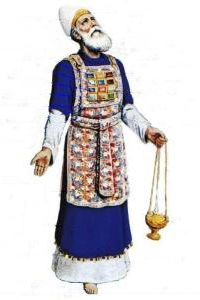
\includegraphics[width=50mm,scale=1.5]{Extras/Melchisedec.jpg}
\vspace{0.4in}  % Create a title for the document and write it in bold font
\LARGE{\textbf{\date}} % Again, do a line break
\linebreak 
% Create a subtitle \large{with Outlines, Statistics, Cross References, and Notes}
\vspace{0.5in}
\begin{flushleft}
\LARGE{Day \#71: Saturday, 12 March 2022  \\}\vspace{0.25in}
\LARGE{Joshua 19-21 Psalm 71 Proverb 12}
\end{flushleft}
\vspace{0.6in}
\bigskip

\normalsize{Xenia, Oh.\\}
\normalsize{created: \today}
\vspace{1.3in}

\end{flushright}
\end{titlepage}

\newpage 
\tableofcontents\hypertarget{TOC}{}
\listoffigures
\listoftables

\hyphenation{A-bim-e-lech bre-thren E-phra-im  Gib-e-o-nites Jer-u-sa-lem through-out Phil-i-stines The-o-phil-us Am-a-le-kites ven-geance Mesh-el-e-mi-ah onan-ism Phar-a-oh thoughts grev-ous-ness Hach-a-liah adul-ter-er Shad-rach}

%%%%%%%%%%%%%%%%% EXTRA COLORS
%%%%%%%%%%%%%%%%% EXTRA COLORS
%%%%%%%%%%%%%%%%% EXTRA COLORS
\definecolor{champagne}{rgb}{0.97,0.91,0.81}
\definecolor{bone}{rgb}{0.89,0.85,0.79}

\definecolor{ForestGreen}{rgb}{0.00,0.29,0.098}
\definecolor{GIVING}{cmyk}{1,0.0,0.72,.1}

\definecolor{MLPE}{cmyk}{1,1,0,.45}
\definecolor{SOCCER}{cmyk}{.77, 0, .42, .49}
\definecolor{PAYBILL}{cmyk}{0,0.83,0.76,0.07}
\definecolor{SERMON}{cmyk}{.14,.9,0,.30} % aka seance \href{http://www.flatuicolorpicker.com/purple-cmyk-color-model/}{seance}
\definecolor{BIBLE}{cmyk}{0,.17,.74,.17}
\definecolor{WORKBLUE}{cmyk}{1, .5, 0, .6}
\definecolor{myOrange}{cmyk}{0, .4, .98, .03}
\definecolor{myTan}{cmyk}{0.0,.07,.17,.10}
\definecolor{myRed}{cmyk}{0,1,1,0}
\definecolor{myWhite}{cmyk}{0,0,0,0}
\definecolor{BLUESoD}{cmyk}{.97,.84,0,.04}
\definecolor{WHITE}{cmyk}{0,0,0,0}
\definecolor{OLDGOLD}{cmyk}{0.05,0.3,1.00,0}
\definecolor{CASTLETON}{cmyk}{1,0,0.31,0.66}
\definecolor{cadmiumgreen}{rgb}{0.0, 0.42, 0.24}
\definecolor{jungle}{rgb}{0.203,0.4882,0.1718}
\definecolor{MYGOLD}{rgb}{1,.84,0}

\definecolor{MYLIGHTGRAY}{rgb}{.85,.85,.85}

\definecolor{codegreen}{rgb}{0,0.6,0}
\definecolor{codegray}{rgb}{0.5,0.5,0.5}
\definecolor{codepurple}{rgb}{0.58,0,0.82}
\definecolor{backcolour}{rgb}{0.95,0.95,0.92}


\mdfdefinestyle{MyFrame}{%
    linecolor=blue,
    outerlinewidth=2pt,
    roundcorner=5pt,
    innertopmargin=\baselineskip,
    innerbottommargin=\baselineskip,
    innerrightmargin=10pt,
    innerleftmargin=10pt,
    backgroundcolor=gray!25!white}


\mdfdefinestyle{MyFrame2}{%
    linecolor=black,
    outerlinewidth=2pt,
    roundcorner=5pt,
    innertopmargin=\baselineskip,
    innerbottommargin=\baselineskip,
    innerrightmargin=10pt,
    innerleftmargin=10pt,
    backgroundcolor=yellow!25!white}


%%%%%
%% for PFTTIS list
%%%%%

%%% And Joseph said unto
\index[PFTTIS]{And Joseph said unto!Genesis!Gen 40:008}
\index[PFTTIS]{And Joseph said unto!Genesis!Gen 40:012}
\index[PFTTIS]{And Joseph said unto!Genesis!Gen 41:025}
\index[PFTTIS]{And Joseph said unto!Genesis!Gen 42:014}
\index[PFTTIS]{And Joseph said unto!Genesis!Gen 42:018}
\index[PFTTIS]{And Joseph said unto!Genesis!Gen 44:015}
\index[PFTTIS]{And Joseph said unto!Genesis!Gen 45:003}
\index[PFTTIS]{And Joseph said unto!Genesis!Gen 45:004}
\index[PFTTIS]{And Joseph said unto!Genesis!Gen 46:031}
\index[PFTTIS]{And Joseph said unto!Genesis!Gen 48:009}
\index[PFTTIS]{And Joseph said unto!Genesis!Gen 48:018}
\index[PFTTIS]{And Joseph said unto!Genesis!Gen 50:019}
\index[PFTTIS]{And Joseph said unto!Genesis!Gen 50:024}


%%% a shadow
\index[PFTTIS]{a shadow!1Chronicles!1Chr 029:15}
\index[PFTTIS]{a shadow!Job!Job 008:09}
\index[PFTTIS]{a shadow!Job!Job 014:02}
\index[PFTTIS]{a shadow!Job!Job 017:07}
\index[PFTTIS]{a shadow!Psalm!Psa 102:011}
\index[PFTTIS]{a shadow!Psalm!Psa 144:004}
\index[PFTTIS]{a shadow!Ecclesiastes!Eccl 006:012}
\index[PFTTIS]{a shadow!Ecclesiastes!Eccl 008:013}
\index[PFTTIS]{a shadow!Isaiah!Isa 04:006}
\index[PFTTIS]{a shadow!Isaiah!Isa 25:004}
\index[PFTTIS]{a shadow!Jonah!Jnh 04:06}
\index[PFTTIS]{a shadow!Colossians!Col 02:017}
\index[PFTTIS]{a shadow!Hebews!Heb 10:001}

%%% blessed is the man
\index[PFTTIS]{blessed is the man!Psalm!Psa 001:001}
\index[PFTTIS]{blessed is the man!Psalm!Psa 032:002}
\index[PFTTIS]{blessed is the man!Psalm!Psa 034:008}
\index[PFTTIS]{blessed is the man!Psalm!Psa 065:004}
\index[PFTTIS]{blessed is the man!Psalm!Psa 084:005}
\index[PFTTIS]{blessed is the man!Psalm!Psa 084:012}
\index[PFTTIS]{blessed is the man!Psalm!Psa 094:012}
\index[PFTTIS]{blessed is the man!Psalm!Psa 112:001}
\index[PFTTIS]{blessed is the man!Proverbs!Pro 008:034}
\index[PFTTIS]{blessed is the man!Isaiah!Isa 056:002}
\index[PFTTIS]{blessed is the man!Jeremiah!Jer 017:007}
\index[PFTTIS]{blessed is the man!Romans!Rom 004:008}
\index[PFTTIS]{blessed is the man!James!Jam 001:012}


%%% carry them
\index[PFTTIS]{carry them!Leviticus!Lev 14:045}
\index[PFTTIS]{carry them!Numbers!Num 11:012}
\index[PFTTIS]{carry them!Joshua!Jsh 04:003}
\index[PFTTIS]{carry them!1Samuel!1Sam 20:040}
\index[PFTTIS]{carry them!1Kings!1Kng 08:046}
\index[PFTTIS]{carry them!2Chronicles!2Chr 06:036}
\index[PFTTIS]{carry them!Ezra!Ezra 05:015}
\index[PFTTIS]{carry them!Isaiah!Isa 40:011}
\index[PFTTIS]{carry them!Isaiah!Isa 41:016}
\index[PFTTIS]{carry them!Isaiah!Isa 57:013}
\index[PFTTIS]{carry them!Jeremiah!Jer 20:004}
\index[PFTTIS]{carry them!Jeremiah!Jer 20:005}
\index[PFTTIS]{carry them!Jeremiah!Jer 43:012}


\index[PFTTIS]{good tidings!2Samuel!2Sam 18:027}
\index[PFTTIS]{good tidings!1Kings!1Ki 01:042}
\index[PFTTIS]{good tidings!2Kings!2Ki 07:009 (2x)}
\index[PFTTIS]{good tidings!Isaiah!Isa 40:009 (2x)}
\index[PFTTIS]{good tidings!Isaiah!Isa 41:007}
\index[PFTTIS]{good tidings!Isaiah!Isa 52:007}
\index[PFTTIS]{good tidings!Isaiah!Isa 61:001}
\index[PFTTIS]{good tidings!Nahum!Nah 01:005}
\index[PFTTIS]{good tidings!Luke!Lk 02:010}
\index[PFTTIS]{good tidings!1Thessalonians!1Thess 03:006}


%%% dead body
\index[PFTTIS]{dead body!Leviticus!Lev 21:011}
\index[PFTTIS]{dead body!Numbers!Num 06:006}
\index[PFTTIS]{dead body!Numbers!Num 09:006}
\index[PFTTIS]{dead body!Numbers!Num 09:007}
\index[PFTTIS]{dead body!Numbers!Num 09:010}
\index[PFTTIS]{dead body!Numbers!Num 09:011}
\index[PFTTIS]{dead body!Numbers!Num 09:013}
\index[PFTTIS]{dead body!Numbers!Num 09:016}
\index[PFTTIS]{dead body!2Kings!2Ki 08:005}
\index[PFTTIS]{dead body!Isaiah!Isa 26:019}
\index[PFTTIS]{dead body!Jeremiah!Jer 26:023}
\index[PFTTIS]{dead body!Jeremiah!Jer 36:030}
\index[PFTTIS]{dead body!Haggai!Hag 02:013}

%%% great sea
\index[PFTTIS]{great sea!Numbers!Num 34:006}
\index[PFTTIS]{great sea!Numbers!Num 34:007}
\index[PFTTIS]{great sea!Joshua!Jos 01:004}
\index[PFTTIS]{great sea!Joshua!Jos 09:001}
\index[PFTTIS]{great sea!Joshua!Jos 15:012}
\index[PFTTIS]{great sea!Joshua!Jos 15:047}
\index[PFTTIS]{great sea!Joshua!Jos 23:004}
\index[PFTTIS]{great sea!Ezekiel!Eze 47:010}
\index[PFTTIS]{great sea!Ezekiel!Eze 47:015}
\index[PFTTIS]{great sea!Ezekiel!Eze 47:019}
\index[PFTTIS]{great sea!Ezekiel!Eze 47:020}
\index[PFTTIS]{great sea!Ezekiel!Eze 48:028}
\index[PFTTIS]{great sea!Daniel!Dan 07:002}


%%% have forsaken me
\index[PFTTIS]{have forsaken me!Judges!Jdg 10:013}
\index[PFTTIS]{have forsaken me!1Samuel!1Sam 08:008}
\index[PFTTIS]{have forsaken me!1Kings!1Ki 11:033}
\index[PFTTIS]{have forsaken me!2Kings!2Ki 22:017}
\index[PFTTIS]{have forsaken me!2Chronicles!2Chr 12:005}
\index[PFTTIS]{have forsaken me!2Chronicles!2Chr 34:025}
\index[PFTTIS]{have forsaken me!Jeremiah!Jer 01:016}
\index[PFTTIS]{have forsaken me!Jeremiah!Jer 02:013}
\index[PFTTIS]{have forsaken me!Jeremiah!Jer 05:007}
\index[PFTTIS]{have forsaken me!Jeremiah!Jer 05:019}
\index[PFTTIS]{have forsaken me!Jeremiah!Jer 16:011 (2x)}
\index[PFTTIS]{have forsaken me!Jeremiah!Jer 19:004}

%%% no king
\index[PFTTIS]{no king!Judges!Jdg 17:06}
\index[PFTTIS]{no king!Judges!Jdg 18:01}
\index[PFTTIS]{no king!Judges!Jdg 19:01}
\index[PFTTIS]{no king!Judges!Jdg 21:25}
\index[PFTTIS]{no king!1Kings!1Ki 22:47}
\index[PFTTIS]{no king!2Kings!2Ki 23:25}
\index[PFTTIS]{no king!Nehemiah!Neh 13:26}
\index[PFTTIS]{no king!Psalms!Psa 033:016}
\index[PFTTIS]{no king!Proverbs!Pro 30:27}
\index[PFTTIS]{no king!Daniel!Dan 02:10}
\index[PFTTIS]{no king!Hosea!Hos 10:03}
\index[PFTTIS]{no king!Micah!Mic 04:09}
\index[PFTTIS]{no king!John!Jhn 19:15}


%%% rebellious house
\index[PFTTIS]{rebellious house!Exodus!Exo 02:005}
\index[PFTTIS]{rebellious house!Exodus!Exo 02:006}
\index[PFTTIS]{rebellious house!Exodus!Exo 02:008}
\index[PFTTIS]{rebellious house!Exodus!Exo 03:009}
\index[PFTTIS]{rebellious house!Exodus!Exo 03:026}
\index[PFTTIS]{rebellious house!Exodus!Exo 03:027}
\index[PFTTIS]{rebellious house!Exodus!Exo 12:002 (2x)}
\index[PFTTIS]{rebellious house!Exodus!Exo 12:003}
\index[PFTTIS]{rebellious house!Exodus!Exo 12:009}
\index[PFTTIS]{rebellious house!Exodus!Exo 12:025}
\index[PFTTIS]{rebellious house!Exodus!Exo 17:012}
\index[PFTTIS]{rebellious house!Exodus!Exo 24:003}

%%% seek him
\index[PFTTIS]{seek him!Deuteronomy!Deu 04:029}\index[PFTTIS]{seek him!1Samuel!1Sam 23:025}
\index[PFTTIS]{seek him!1Chronicles!1Chr 28:009}
\index[PFTTIS]{seek him!2Chronicles!1Chr 15:002}
\index[PFTTIS]{seek him!Ezra!Ezr 08:022}
\index[PFTTIS]{seek him!Psalms!Psa 022:026}
\index[PFTTIS]{seek him!Psalms!Psa 024:006}
\index[PFTTIS]{seek him!Psalms!Psa 119:002}
\index[PFTTIS]{seek him!SoS!SoS 03:002}
\index[PFTTIS]{seek him!SoS!SoS 06:001}
\index[PFTTIS]{seek him!Hosea!Hos 07:010}
\index[PFTTIS]{seek him!Amos!Amo 05:008}
\index[PFTTIS]{seek him!Hebrews!Heb 11:0063}


%%% seek ye
\index[PFTTIS]{seek ye!Isaiah!Isa 34:016}
\index[PFTTIS]{seek ye!Isaiah!Isa 45:019}
\index[PFTTIS]{seek ye!Isaiah!Isa 55:006}
\index[PFTTIS]{seek ye!Amos!Amos 5:004}
\index[PFTTIS]{seek ye!John!John 1:38}
\index[PFTTIS]{seek ye!John!John 18:4}
\index[PFTTIS]{seek ye!John!John 18:7}
\index[PFTTIS]{seek ye!Matthew!Matt 6:33}
\index[PFTTIS]{seek ye!Numbers!Num 16:10}
\index[PFTTIS]{seek ye!Luke!Luke 12:31}
\index[PFTTIS]{seek ye!Luke!Luke 24:5}
\index[PFTTIS]{seek ye!Psalm!Psa 27:8}
\index[PFTTIS]{seek ye!Zephaniah!Zeph 2:3}

%%% the uncircumcised
\index[PFTTIS]{the uncircumcised!Genesis!Gen 17:014}
\index[PFTTIS]{the uncircumcised!Judges!Jdg 14:003}
\index[PFTTIS]{the uncircumcised!Judges!Jdg 15:018}
\index[PFTTIS]{the uncircumcised!2Samuel!2Sam 01:020}
\index[PFTTIS]{the uncircumcised!Isaiah!Isa 02:001}
\index[PFTTIS]{the uncircumcised!Jeremiah!Jer 09:025}
\index[PFTTIS]{the uncircumcised!Ezekiel!Eze 28:010}
\index[PFTTIS]{the uncircumcised!Ezekiel!Eze 31:018}
\index[PFTTIS]{the uncircumcised!Ezekiel!Eze 32:019}
\index[PFTTIS]{the uncircumcised!Ezekiel!Eze 32:027}
\index[PFTTIS]{the uncircumcised!Ezekiel!Eze 32:028}
\index[PFTTIS]{the uncircumcised!Ezekiel!Eze 32:029}
\index[PFTTIS]{the uncircumcised!Ezekiel!Eze 32:032}

%%% worship him
\index[PFTTIS]{worship him!Psalms!Psa 97:007}
\index[PFTTIS]{worship him!Zephaniah!Zeph 02:011}
\index[PFTTIS]{worship him!Matthew!Matt 02:002}
\index[PFTTIS]{worship him!Matthew!Matt 02:008}
\index[PFTTIS]{worship him!John!John 04:023}
\index[PFTTIS]{worship him!John!John 04:024 (2x)} 
\index[PFTTIS]{worship him!Acts!Acts 17:023}
\index[PFTTIS]{worship him!Hebrews!Heb 01:006}
\index[PFTTIS]{worship him!Revelation!Rev 04:010}
\index[PFTTIS]{worship him!Revelation!Rev 13:008}
\index[PFTTIS]{worship him!Revelation!Rev 14:007}
\index[PFTTIS]{worship him!Revelation!Rev 19:010}


%%%%%
%% for PFTTIS list
%%%%%

%%% afflictions
\index[WFTTIS]{afflictions!Psalms!Psa 34:019}
\index[WFTTIS]{afflictions!Psalms!Psa 132:001}
\index[WFTTIS]{afflictions!Acts!Acts 07:010}
\index[WFTTIS]{afflictions!Acts!Acts 20:023}
\index[WFTTIS]{afflictions!2Corinthians!2Cor 06:004}
\index[WFTTIS]{afflictions!Colossians!Col 01:024}
\index[WFTTIS]{afflictions!1Thessalonians!1Thess 03:003}
\index[WFTTIS]{afflictions!2Timothy!2Tim 01:008}
\index[WFTTIS]{afflictions!2Timothy!2Tim 03:011}
\index[WFTTIS]{afflictions!2Timothy!2Tim 04:005}
\index[WFTTIS]{afflictions!Hebrews!Heb 10:032}
\index[WFTTIS]{afflictions!Hebrews!Heb 10:033}
\index[WFTTIS]{afflictions!1Peter!1Pet 05:009}

%%% acsend
\index[WFTTIS]{acsend!Joshua!Jos 06:05}
\index[WFTTIS]{acsend!Psalm!Psa 024:003}
\index[WFTTIS]{acsend!Psalm!Psa 135:007}
\index[WFTTIS]{acsend!Psalm!Psa 139:008}
\index[WFTTIS]{acsend!Isaiah!Isa 14:013}
\index[WFTTIS]{acsend!Isaiah!Isa 14:014}
\index[WFTTIS]{acsend!Jeremiah!Jer 10:013}
\index[WFTTIS]{acsend!Jeremiah!Jer 51:016}
\index[WFTTIS]{acsend!Ezekiel!Eze 38:009}
\index[WFTTIS]{acsend!John!John 06:062}
\index[WFTTIS]{acsend!John!John 20:017}
\index[WFTTIS]{acsend!Romans!Rom 10:006}
\index[WFTTIS]{acsend!Revelation!Rev 17:008}

%%% Assyrian
\index[WFTTIS]{Assyrian!Isaiah!Isa 10:005}
\index[WFTTIS]{Assyrian!Isaiah!Isa 10:024}
\index[WFTTIS]{Assyrian!Isaiah!Isa 14:025}
\index[WFTTIS]{Assyrian!Isaiah!Isa 19:023}
\index[WFTTIS]{Assyrian!Isaiah!Isa 23:013}
\index[WFTTIS]{Assyrian!Isaiah!Isa 30:031}
\index[WFTTIS]{Assyrian!Isaiah!Isa 31:008}
\index[WFTTIS]{Assyrian!Isaiah!Isa 52:004}
\index[WFTTIS]{Assyrian!Ezekiel!Eze 31:003}
\index[WFTTIS]{Assyrian!Hosea!Hos 05:013}
\index[WFTTIS]{Assyrian!Hosea!Hos 11:005}
\index[WFTTIS]{Assyrian!Micah!Hos 05:005}
\index[WFTTIS]{Assyrian!Micah!Hos 05:006}

%%% blot
\index[WFTTIS]{blot!Exodus!Exo 32:032}
\index[WFTTIS]{blot!Exodus!Exo 32:033}
\index[WFTTIS]{blot!Numbers!Num 05:026}
\index[WFTTIS]{blot!Deuteronomy!Deut 09:014}
\index[WFTTIS]{blot!Deuteronomy!Deut 25:019}
\index[WFTTIS]{blot!Deuteronomy!Deut 29:020}
\index[WFTTIS]{blot!2Kings!2Ki 14:027}
\index[WFTTIS]{blot!Job!Job 31:007}
\index[WFTTIS]{blot!Psalms!Psa 51:001}
\index[WFTTIS]{blot!Psalms!Psa 51:009}
\index[WFTTIS]{blot!Proverbs!Pro 09:007}
\index[WFTTIS]{blot!Jeremiah!Jer 18:023}
\index[WFTTIS]{blot!Revelation!Rev 03:005}


%%% chain
\index[WFTTIS]{chain!Genesis!Gen 41:042}
\index[WFTTIS]{chain!1Kings!1Ki 07:017}
\index[WFTTIS]{chain!Psalms!Psa 73:006}
\index[WFTTIS]{chain!SoS!Sos 04:009}
\index[WFTTIS]{chain!Lamentations!Lam 03:007}
\index[WFTTIS]{chain!Ezekiel!Eze 07:023}
\index[WFTTIS]{chain!Ezekiel!Eze 16:011}
\index[WFTTIS]{chain!Daniel!Dan 05:007}
\index[WFTTIS]{chain!Daniel!Dan 05:016}
\index[WFTTIS]{chain!Daniel!Dan 05:029}
\index[WFTTIS]{chain!Acts!Acts 28:020}
\index[WFTTIS]{chain!2Timothy!2Tim 01:016}
\index[WFTTIS]{chain!Revelation!Rev 20:001}


%%% controversy
\index[WFTTIS]{controversy!Deuteronomy!Deu 17:008}
\index[WFTTIS]{controversy!Deuteronomy!Deu 19:017}
\index[WFTTIS]{controversy!Deuteronomy!Deu 21:005}
\index[WFTTIS]{controversy!Deuteronomy!Deu 25:001}
\index[WFTTIS]{controversy!2Samuel!2Sam 15:002}
\index[WFTTIS]{controversy!Isaiah!Isa 34:008}
\index[WFTTIS]{controversy!Jeremiah!Jer 25:031}
\index[WFTTIS]{controversy!Ezekiel!Eze 44:024}
\index[WFTTIS]{controversy!Hosea!Hos 04:001}
\index[WFTTIS]{controversy!Hosea!Hos 12:002}
\index[WFTTIS]{controversy!Micah!Mic 06:002 (2x)}
\index[WFTTIS]{controversy!1Timothy!1Tim 03:016}


%%% Dagon/Dagon's
\index[WFTTIS]{Dagon!Judges!Jdg 16:023}
\index[WFTTIS]{Dagon!1Samuel!1Sam 05:002 (2x)}
\index[WFTTIS]{Dagon!1Samuel!1Sam 05:003 (2x)}
\index[WFTTIS]{Dagon!1Samuel!1Sam 05:004 (3x)}
\index[WFTTIS]{Dagon!1Samuel!1Sam 05:005 (3x)}
\index[WFTTIS]{Dagon!1Samuel!1Sam 05:007}
\index[WFTTIS]{Dagon!1Chronicles!1Chr 10:010}

%%% disobedient
\index[WFTTIS]{disobedient!1Kings!1Ki 13:026}
\index[WFTTIS]{disobedient!Nehemiah!Neh 09:026}
\index[WFTTIS]{disobedient!Luke!Luke 01:017}
\index[WFTTIS]{disobedient!Acts!Acts 26:019}
\index[WFTTIS]{disobedient!Romans!Rom 01:030}
\index[WFTTIS]{disobedient!Romans!Rom 10:021}
\index[WFTTIS]{disobedient!1Timothy!1Tim 01:009}
\index[WFTTIS]{disobedient!2Timothy!2Tim 03:002}
\index[WFTTIS]{disobedient!Titus!Titus 01:016}
\index[WFTTIS]{disobedient!Titus!Titus 03:003}
\index[WFTTIS]{disobedient!1Peter!1Pet 02:007}
\index[WFTTIS]{disobedient!1Peter!1Pet 02:008}
\index[WFTTIS]{disobedient!1Peter!1Pet 03:020}


%%% doubt
\index[WFTTIS]{doubt!Genesis!Gen 37:033}
\index[WFTTIS]{doubt!Deuteronomy!Deu 28:066}
\index[WFTTIS]{doubt!Job!Job 12:002}
\index[WFTTIS]{doubt!Matthew!Matt 14:031}
\index[WFTTIS]{doubt!Matthew!Matt 21:021}
\index[WFTTIS]{doubt!Mark!Mk 11:023}
\index[WFTTIS]{doubt!Luke!Lk 11:020}
\index[WFTTIS]{doubt!John!Jhn 10:024}
\index[WFTTIS]{doubt!Acts!Acts 02:012}
\index[WFTTIS]{doubt!Acts!Acts 28:004}
\index[WFTTIS]{doubt!1Corinthians!1Cor 09:010}
\index[WFTTIS]{doubt!Galatians!Gal 04:020}
\index[WFTTIS]{doubt!1John!1Jhn 02:019}


%%% dungeon
\index[WFTTIS]{dungeon!Genesis!Gen 40:015}
\index[WFTTIS]{dungeon!Genesis!Gen 41:014}
\index[WFTTIS]{dungeon!Exodus!Exo 12:029}
\index[WFTTIS]{dungeon!Jeremiah!Jer 37:016}
\index[WFTTIS]{dungeon!Jeremiah!Jer 38:006 (2x)}
\index[WFTTIS]{dungeon!Jeremiah!Jer 38:007}
\index[WFTTIS]{dungeon!Jeremiah!Jer 38:009}
\index[WFTTIS]{dungeon!Jeremiah!Jer 38:010}
\index[WFTTIS]{dungeon!Jeremiah!Jer 38:011}
\index[WFTTIS]{dungeon!Jeremiah!Jer 38:013}
\index[WFTTIS]{dungeon!Lamentations!Lam 03:053}
\index[WFTTIS]{dungeon!Lamentations!Lam 03:055}


%%% error
\index[WFTTIS]{error!2Samuel!2Sam 06:007}
\index[WFTTIS]{error!Job!Job 19:004}
\index[WFTTIS]{error!Ecclesiastes!Ecc 05:006}
\index[WFTTIS]{error!Ecclesiastes!Ecc 10:005}
\index[WFTTIS]{error!Isaiah!Isa 32:006}
\index[WFTTIS]{error!Daniel!Dan 06:004}
\index[WFTTIS]{error!Matthew!Matt 27:064}
\index[WFTTIS]{error!Romans!Rom 01:027}
\index[WFTTIS]{error!James!Jam 05:020}
\index[WFTTIS]{error!2Peter!2Pet 02:018}
\index[WFTTIS]{error!2Peter!2Pet 03:017}
\index[WFTTIS]{error!1John!1Jn 04:006}
\index[WFTTIS]{error!Jude!Jude 01:011}

%%% fourish
\index[WFTTIS]{fourish!Psalms!Psa 072:007}
\index[WFTTIS]{fourish!Psalms!Psa 072:016}
\index[WFTTIS]{fourish!Psalms!Psa 092:007}
\index[WFTTIS]{fourish!Psalms!Psa 092:012}
\index[WFTTIS]{fourish!Psalms!Psa 092:013}
\index[WFTTIS]{fourish!Psalms!Psa 132:018}
\index[WFTTIS]{fourish!Proverbs!Pro 11:28}
\index[WFTTIS]{fourish!Proverbs!Pro 14:11}
\index[WFTTIS]{fourish!Ecclesiastes!Ecc 12:05}
\index[WFTTIS]{fourish!SongOfSolomon!SOS 07:12}
\index[WFTTIS]{fourish!Isaiah!Isa 17:11}
\index[WFTTIS]{fourish!Isaiah!Isa 66:14}
\index[WFTTIS]{fourish!Ezekiel!Eze 17:24}




%%% giants
\index[WFTTIS]{giants!Genesis!Gen 06:004}
\index[WFTTIS]{giants!Numbers!Num 13:033}
\index[WFTTIS]{giants!Deuteronomy!Deut 02:011}
\index[WFTTIS]{giants!Deuteronomy!Deut 02:021}
\index[WFTTIS]{giants!Deuteronomy!Deut 03:011}
\index[WFTTIS]{giants!Deuteronomy!Deut 03:013}
\index[WFTTIS]{giants!Joshua!Josh 12:004}
\index[WFTTIS]{giants!Joshua!Josh 13:012}
\index[WFTTIS]{giants!Joshua!Josh 15:008}
\index[WFTTIS]{giants!Joshua!Josh 17:015}
\index[WFTTIS]{giants!Joshua!Josh 16:016}

%%% good man
\index[WFTTIS]{good man!2 Samuel!2Sa 18:27}
%(1) Psalms 37:23 [5]
%(1) Psalms 112:5 [2]
%(1) Proverbs 12:2 [2]
%(1) Proverbs 13:22 [2]
%(1) Proverbs 14:14 [14]
%(1) Micah 7:2 [2]
%(1) Matthew 12:35 [2]
%(1) Luke 6:45 [2]
%(1) Luke 23:50 [15]
%(1) John 7:12 [17]
%(1) Acts 11:24 [5]
%(1) Romans 5:7 [14]

%%% Hinnom
\index[WFTTIS]{Hinnom!Joshua!Jsh 15:008}
\index[WFTTIS]{Hinnom!Joshua!Jsh 18:016}
\index[WFTTIS]{Hinnom!2Kings!2Ki 23:010}
\index[WFTTIS]{Hinnom!2Chronicles!2Chr 28:003}
\index[WFTTIS]{Hinnom!2Chronicles!2Chr 33:006}
\index[WFTTIS]{Hinnom!Nehemiah!Neh 11:030}
\index[WFTTIS]{Hinnom!Jeremiah!Jer 07:031}
\index[WFTTIS]{Hinnom!Jeremiah!Jer 07:032}
\index[WFTTIS]{Hinnom!Jeremiah!Jer 19:002}
\index[WFTTIS]{Hinnom!Jeremiah!Jer 19:006}
\index[WFTTIS]{Hinnom!Jeremiah!Jer 32:035}

%%% inclined
\index[WFTTIS]{inclined!Judges!Jdg 09:003}
\index[WFTTIS]{inclined!Psalms!Psa 040:001}
\index[WFTTIS]{inclined!Psalms!Psa 116:002}
\index[WFTTIS]{inclined!Psalms!Psa 119:112}
\index[WFTTIS]{inclined!Proverbs!Pro 05:13}
\index[WFTTIS]{inclined!Jeremiah!Jer 07:24}
\index[WFTTIS]{inclined!Jeremiah!Jer 07:26}
\index[WFTTIS]{inclined!Jeremiah!Jer 11:08}
\index[WFTTIS]{inclined!Jeremiah!Jer 17:23}
\index[WFTTIS]{inclined!Jeremiah!Jer 25:04}
\index[WFTTIS]{inclined!Jeremiah!Jer 34:14}
\index[WFTTIS]{inclined!Jeremiah!Jer 35:15}
\index[WFTTIS]{inclined!Jeremiah!Jer 44:05}


%%% laughed
\index[WFTTIS]{laughed!Genesis!Gen 17:017}
\index[WFTTIS]{laughed!Genesis!Gen 18:012}
\index[WFTTIS]{laughed!Genesis!Gen 18:015}
\index[WFTTIS]{laughed!2Kings!2Ki 19:021}
\index[WFTTIS]{laughed!2Chronicles!2Chr 30:010}
\index[WFTTIS]{laughed!Nehemiah!Neh 02:019}
\index[WFTTIS]{laughed!Job!Job 12:004}
\index[WFTTIS]{laughed!Job!Job 29:024}
\index[WFTTIS]{laughed!Isaiah!Isa 37:022}
\index[WFTTIS]{laughed!Ezekiel!Ezek 23:032}
\index[WFTTIS]{laughed!Matthew!Matt 09:024}
\index[WFTTIS]{laughed!Mark!Mk 05:040}
\index[WFTTIS]{laughed!Luke!Lk 08:053}

%%% liar
\index[WFTTIS]{liar!Job!Job 24:025}
\index[WFTTIS]{liar!Proverbs!Pro 17:004}
\index[WFTTIS]{liar!Proverbs!Pro 19:022}
\index[WFTTIS]{liar!Proverbs!Pro 30:006}
\index[WFTTIS]{liar!Jeremiah!Jer 15:018}
\index[WFTTIS]{liar!John!Jhn 08:044}
\index[WFTTIS]{liar!John!Jhn 08:055}
\index[WFTTIS]{liar!Romans!Rom 03:004}
\index[WFTTIS]{liar!1John!1Jhn 01:010}
\index[WFTTIS]{liar!1John!1Jhn 02:004}
\index[WFTTIS]{liar!1John!1Jhn 02:022}
\index[WFTTIS]{liar!1John!1Jhn 04:020}
\index[WFTTIS]{liar!1John!1Jhn 05:010}

%%% palsy
\index[WFTTIS]{palsy!Matthew!Matt 04:024}
\index[WFTTIS]{palsy!Matthew!Matt 08:006}
\index[WFTTIS]{palsy!Matthew!Matt 09:002}
\index[WFTTIS]{palsy!Matthew!Matt 09:006}
\index[WFTTIS]{palsy!Mark!Mk 02:003}
\index[WFTTIS]{palsy!Mark!Mk 02:004}
\index[WFTTIS]{palsy!Mark!Mk 02:005}
\index[WFTTIS]{palsy!Mark!Mk 02:009}
\index[WFTTIS]{palsy!Mark!Mk 02:010}
\index[WFTTIS]{palsy!Luke!Lk 05:018}
\index[WFTTIS]{palsy!Luke!Lk 05:024}
\index[WFTTIS]{palsy!Acts!Acts 09:033}

%%% Profitable
\index[WFTTIS]{profitable!Job!Job 22:002 (2x)}
\index[WFTTIS]{profitable!Ecclesiastes!Ecc 10:010}
\index[WFTTIS]{profitable!Isaiah!Isa 44:010}
\index[WFTTIS]{profitable!Jeremiah!Jer 13:007}
\index[WFTTIS]{profitable!Matthew!Matt 05:029}
\index[WFTTIS]{profitable!Matthew!Matt 05:030}
\index[WFTTIS]{profitable!Acts!Acts 20:020}
\index[WFTTIS]{profitable!1Timothy!1Tim 04:008}
\index[WFTTIS]{profitable!2Timothy!2Tim 03:016}
\index[WFTTIS]{profitable!2Timothy!2Tim 04:011}
\index[WFTTIS]{profitable!Titus!Titus 03:008}
\index[WFTTIS]{profitable!Philemon!Phlm 01:011}

%%% Rechab
\index[WFTTIS]{Rechab!2Samuel!2Sam 04:002}
\index[WFTTIS]{Rechab!2Samuel!2Sam 04:005}
\index[WFTTIS]{Rechab!2Samuel!2Sam 04:006}
\index[WFTTIS]{Rechab!2Samuel!2Sam 04:009}
\index[WFTTIS]{Rechab!2KIngs!2Ki 10:015}
\index[WFTTIS]{Rechab!2KIngs!2Ki 10:023}
\index[WFTTIS]{Rechab!1Chronicles!1Chr 02:055}
\index[WFTTIS]{Rechab!Nehemiah!Neh 03:014}
\index[WFTTIS]{Rechab!Jeremiah!Jer 35:006}
\index[WFTTIS]{Rechab!Jeremiah!Jer 35:008}
\index[WFTTIS]{Rechab!Jeremiah!Jer 35:014}
\index[WFTTIS]{Rechab!Jeremiah!Jer 35:016}
\index[WFTTIS]{Rechab!Jeremiah!Jer 35:019}

%%% serpents
\index[WFTTIS]{serpents!Exodus!Exo 07:012}
\index[WFTTIS]{serpents!Numbers!Num 21:006}
\index[WFTTIS]{serpents!Numbers!Num 21:007}
\index[WFTTIS]{serpents!Deuteronomy!Deu 08:015}
\index[WFTTIS]{serpents!Deuteronomy!Deu 32:024}
\index[WFTTIS]{serpents!Jeremiah!Jer 08:017}
\index[WFTTIS]{serpents!Matthew!Matt 10:016}
\index[WFTTIS]{serpents!Matthew!Matt 23:033}
\index[WFTTIS]{serpents!Mark!Mk 16:018}
\index[WFTTIS]{serpents!Luke!Lk 10:019}
\index[WFTTIS]{serpents!1Corinthians!1Cor 10:009}
\index[WFTTIS]{serpents!James!Jas 03:007}
\index[WFTTIS]{serpents!Revelation!Rev 09:019}

%%% short
\index[WFTTIS]{short!Numbers!Num 11:023}
\index[WFTTIS]{short!2Kings!2Ki 10:032}
\index[WFTTIS]{short!Job!Job 17:012}
\index[WFTTIS]{short!Job!Job 20:005}
\index[WFTTIS]{short!Psalms!Psa 89:047}
\index[WFTTIS]{short!Romans!Rom 03:023}
\index[WFTTIS]{short!Romans!Rom 09:028  (2x)}
\index[WFTTIS]{short!1Corinthians!1Cor 07:029}
\index[WFTTIS]{short!1Thessalonians!1Thess 02:017}
\index[WFTTIS]{short!Hebrews!Heb 04:001}
\index[WFTTIS]{short!Revelation!Rev 12:012}
\index[WFTTIS]{short!Revelation!Rev 17:010}

%%% smiteth
\index[WFTTIS]{smiteth!Exodus!Exo 21:012}
\index[WFTTIS]{smiteth!Exodus!Exo 21:15}
\index[WFTTIS]{smiteth!Deuteronomy!Dt 25:11}
\index[WFTTIS]{smiteth!Deuteronomy!Dt 27:24}
\index[WFTTIS]{smiteth!Joshua!Jsh 15:16}
\index[WFTTIS]{smiteth!Judges!Jdg 15:16}
\index[WFTTIS]{smiteth!2 Samuel!2Sa 05:08}
\index[WFTTIS]{smiteth!1Chronicles!1Chr 11:06}
\index[WFTTIS]{smiteth!Job!1Chr 26:12}
\index[WFTTIS]{smiteth!Isaiah!Isa 09:13}
\index[WFTTIS]{smiteth!Lamentations!Lam 03:30}
\index[WFTTIS]{smiteth!Ezekiel!Eze 07:09}
\index[WFTTIS]{smiteth!Luke!Lk 06:29}



%%% vanities
\index[WFTTIS]{vanities!Deuteronomy!Deut 21:021}
\index[WFTTIS]{vanities!1Kings!1Ki 16:013}
\index[WFTTIS]{vanities!1Kings!1Ki 16:026}
\index[WFTTIS]{vanities!Psalms!Psa 031:006}
\index[WFTTIS]{vanities!Ecclesiastes!Ecc 01:002 (2x)}
\index[WFTTIS]{vanities!Ecclesiastes!Ecc 05:007}
\index[WFTTIS]{vanities!Ecclesiastes!Ecc 12:008}
\index[WFTTIS]{vanities!Jeremiah!Jer 08:019}
\index[WFTTIS]{vanities!Jeremiah!Jer 10:008}
\index[WFTTIS]{vanities!Jeremiah!Jer 14:022}
\index[WFTTIS]{vanities!Jonah!Jnh 02:008}
\index[WFTTIS]{vanities!Acts!Acts 14:015}



%%%%%
%% for PFTTIS list
%%%%%

%%% worm
\index[WFITV]{worm!Exodus!Exo 16:024}
\index[WFITV]{worm!Job!Job 17:014}
\index[WFITV]{worm!Job!Job 24:029}
\index[WFITV]{worm!Job!Job 25:005 (2x)}
\index[WFITV]{worm!Psalms!Psa 022:006}
\index[WFITV]{worm!Isaiah!Isa 14:011}
\index[WFITV]{worm!Isaiah!Isa 41:014}
\index[WFITV]{worm!Isaiah!Isa 51:008}
\index[WFITV]{worm!Isaiah!Isa 66:024}
\index[WFITV]{worm!Jonah!Jnh 04:007}
\index[WFITV]{worm!Mark!Mk 09:044}
\index[WFITV]{worm!Mark!Mk 09:046}
\index[WFITV]{worm!Mark!Mk 09:048}


%\subsubsection{Title}
%\textbf{Introduction:} Isaiah 46 
%\index[speaker]{Speaker!Isaiah 49 (Title}
%\index[series]{Book (Speaker)!IPassage (Title)}
%\index[date]{2017/07/09!Isaiah 49 (Title)}
%\begin{compactenum}[I.]
%    \item  \textbf{Point} \index[scripture]{Isaiah!IPassage} (IPassage)
%\end{compactenum}




  


%\input{02OT-Exodus/ExodusIntroduction}

%\newpage
%\begin{figure}
%\begin{center}
%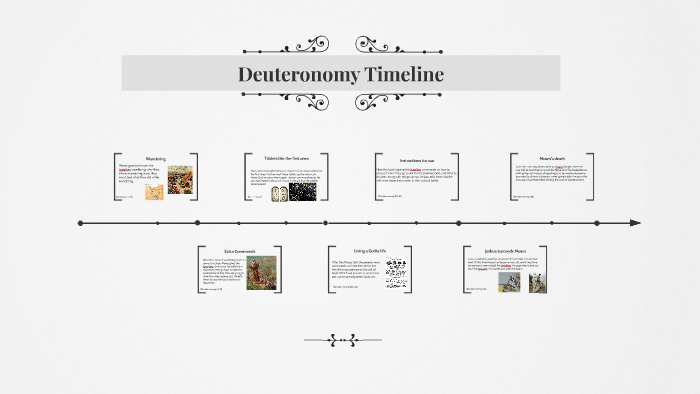
\includegraphics[scale=.7, angle=0]{05OT-Deuteronomy/References/AndrewSmithDeuteronomyTimeline.png}
%\caption[Deuteronomy Timeline by Andrew Smith]{Deuteronomy Timeline by Andrew %Smith}
%\label{fig:Deuteronomy Timeline by Andrew Smith}
%\end{center}
%\end{figure}

\newpage
\begin{figure}
\begin{center}
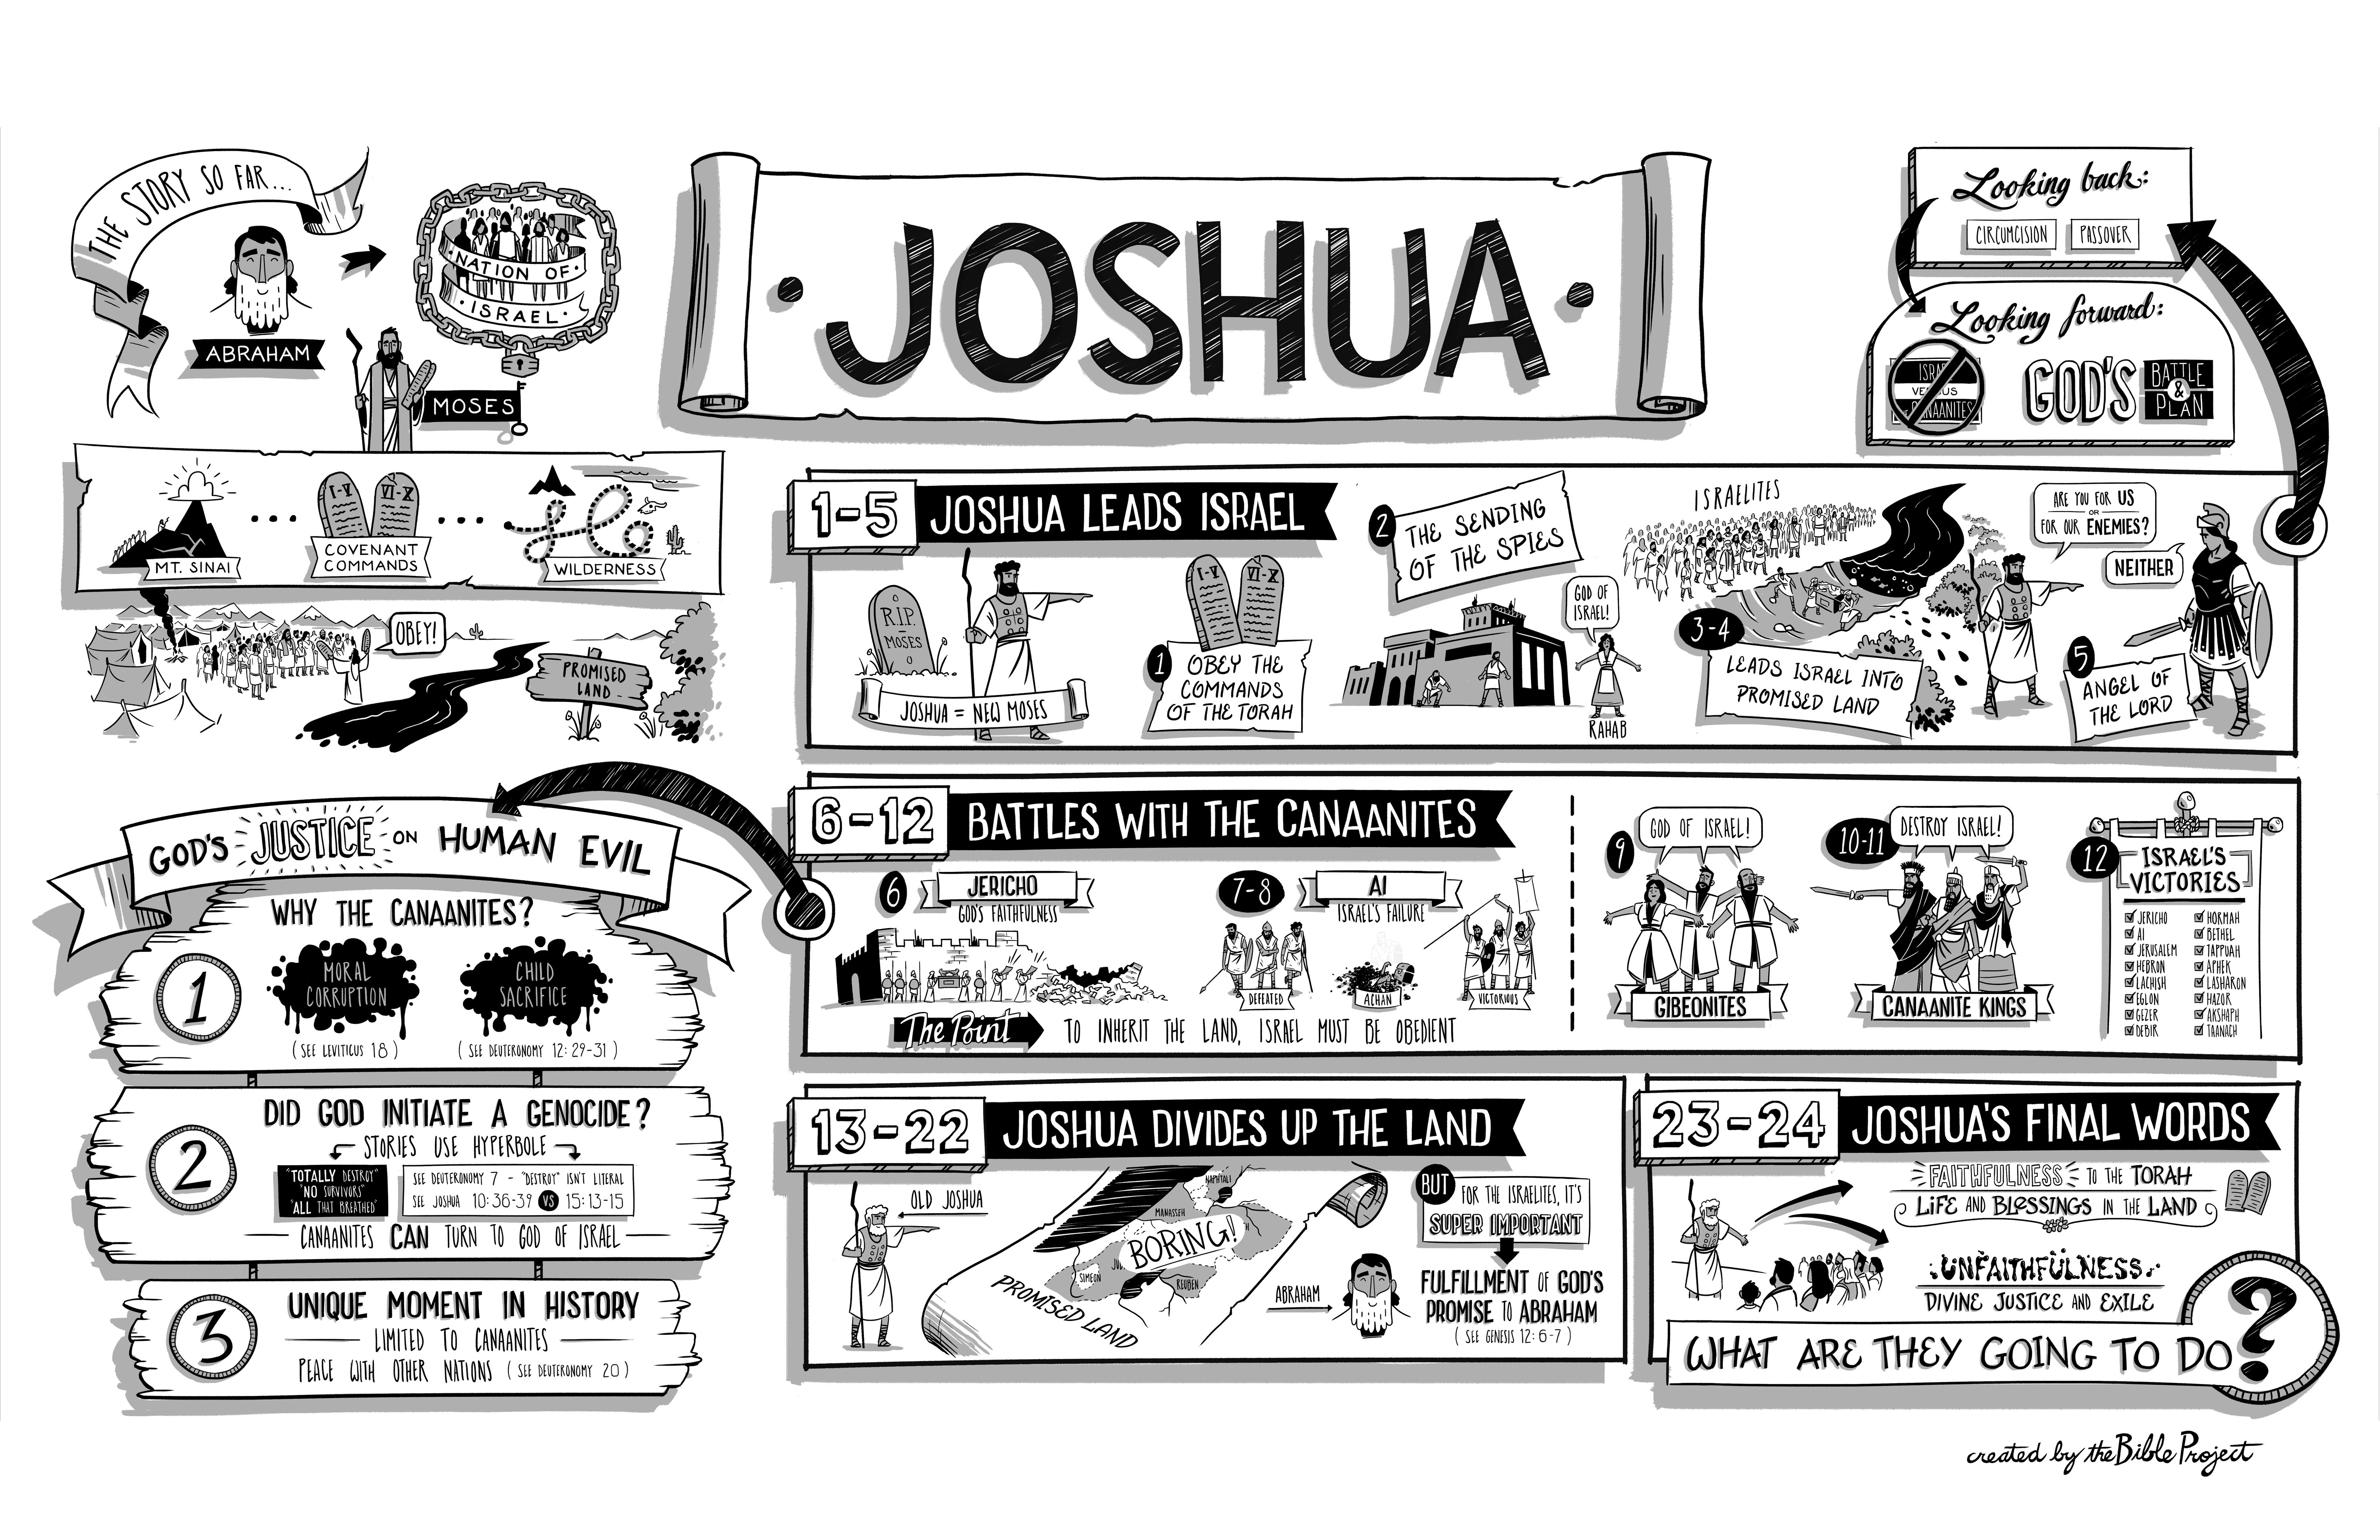
\includegraphics[scale=0.5, angle=90]{06OT-Joshua/References/1.BibleProject-Joshua.jpg}
\caption[Joshua from the Bible Project]{Joshua from the Bible Project}
\label{fig:Joshua from the Bible Project}
\end{center}
\end{figure}

\newpage
\begin{figure}
\begin{center}
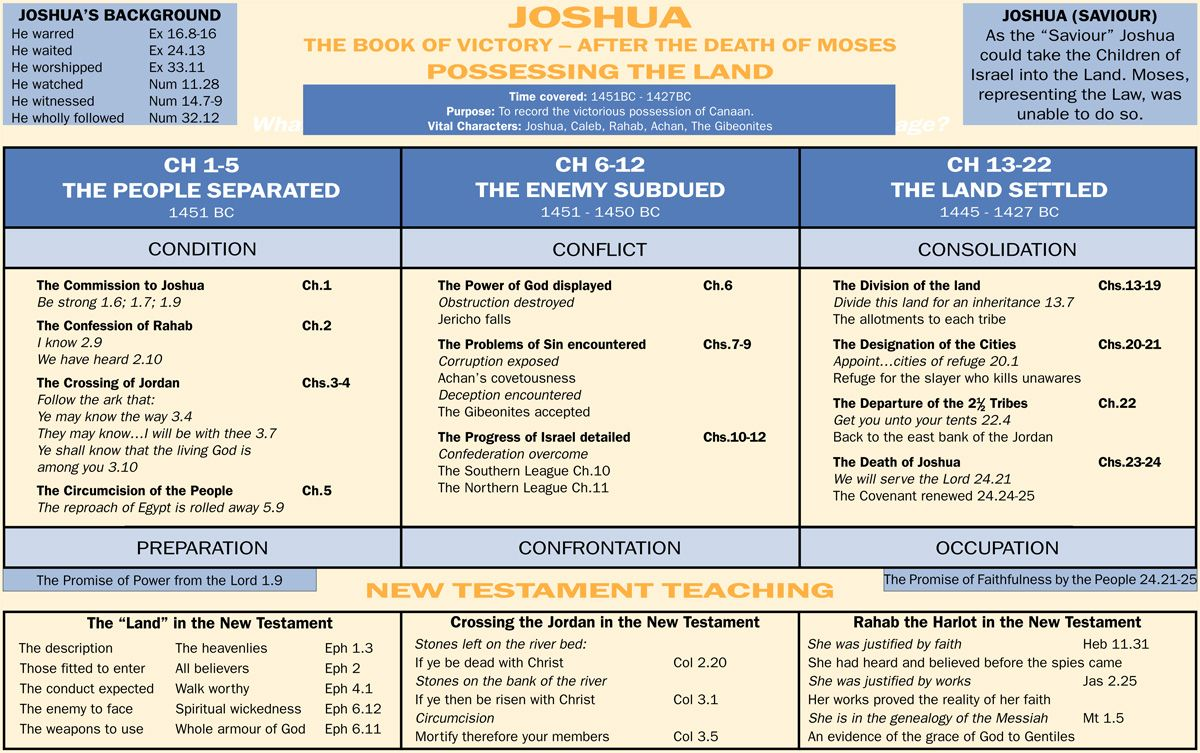
\includegraphics[scale=0.5, angle=90]{06OT-Joshua/References/2.JohnGrant-Joshua.jpg}
\caption[Joshua from John Grant]{Joshua from John Grant}
\label{fig:Joshua from John Grant}
\end{center}
\end{figure}

\newpage
\begin{figure}
\begin{center}
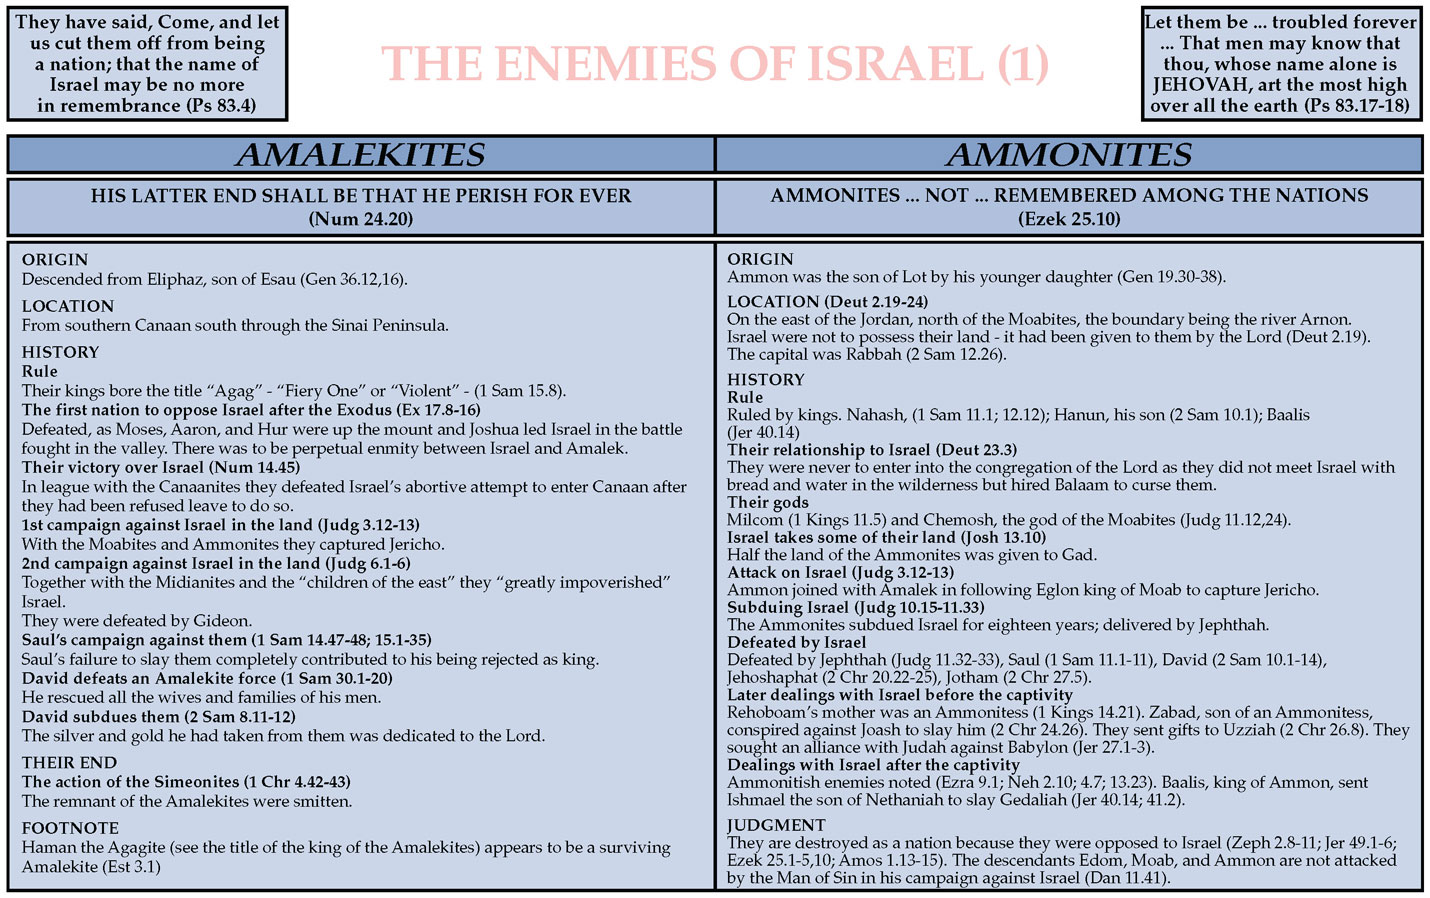
\includegraphics[scale=0.4, angle=90]{06OT-Joshua/References/3.EnemiesOfIsrael1.jpg}
\caption[Enemies of Israel 1]{Enemies of Israel 1}
\label{fig:Enemies of Israel 1}
\end{center}
\end{figure}

\newpage
\begin{figure}
\begin{center}
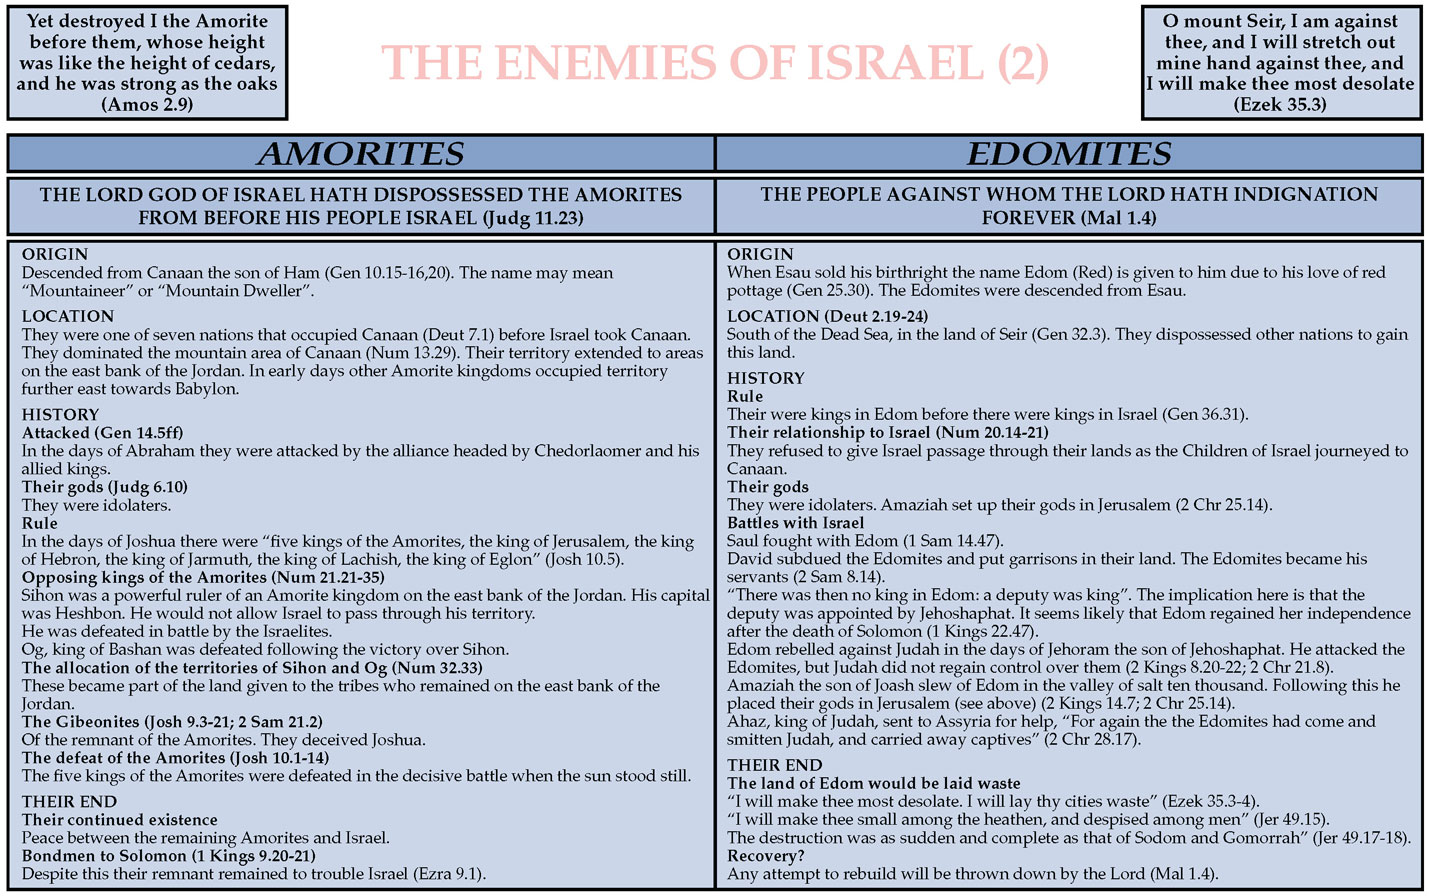
\includegraphics[scale=0.4, angle=90]{06OT-Joshua/References/4.EnemiesOfIsrael2.jpg}
\caption[Enemies of Israel 2]{Enemies of Israel 2}
\label{fig:Enemies of Israel 2}
\end{center}
\end{figure}

\newpage
\begin{figure}
\begin{center}
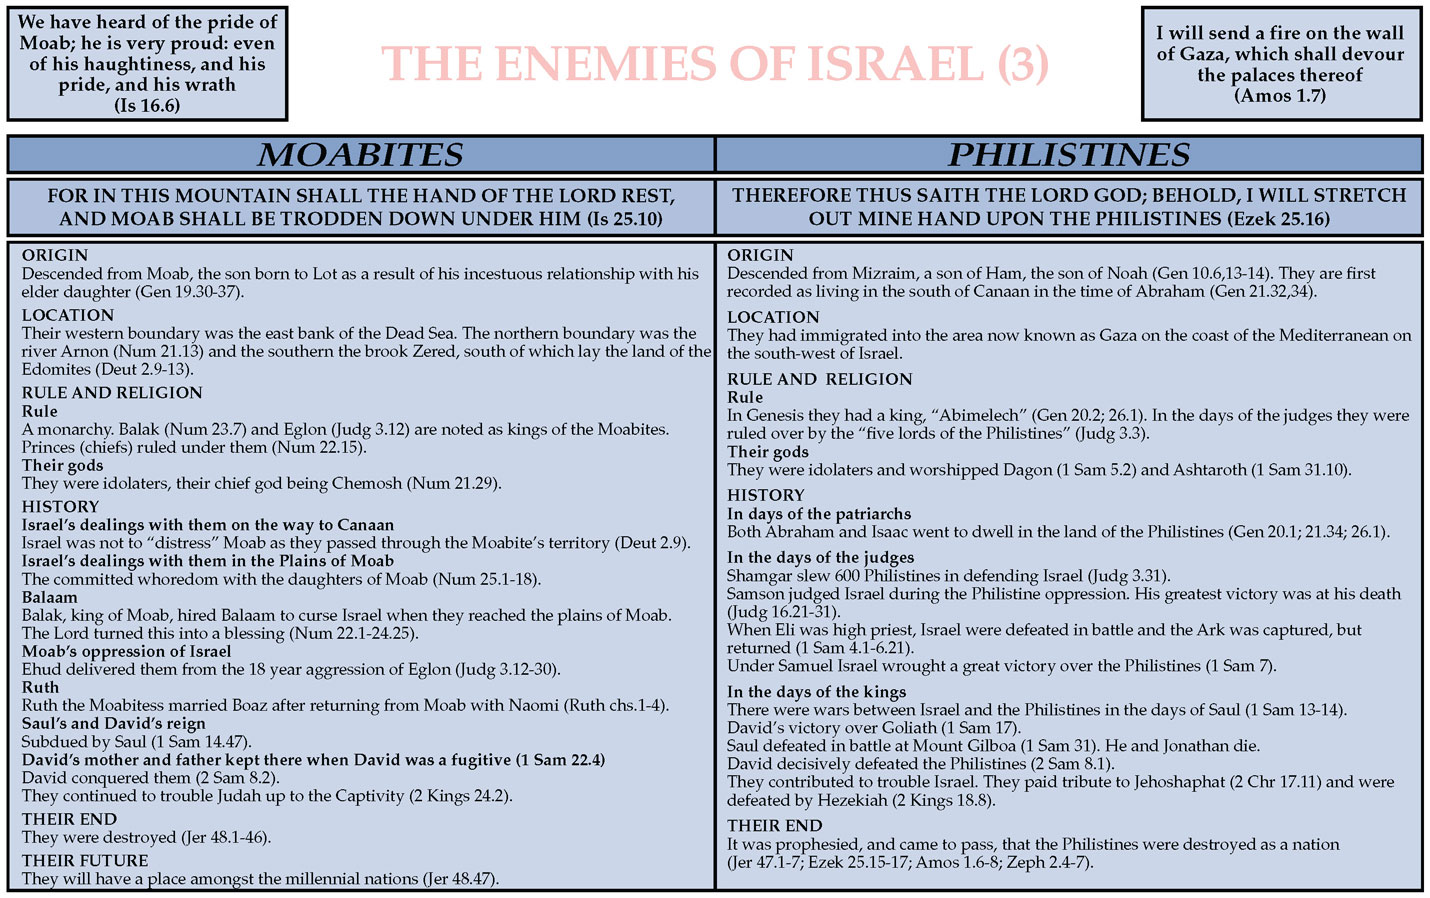
\includegraphics[scale=0.4, angle=90]{06OT-Joshua/References/5.EnemiesOfIsrael3.jpg}
\caption[Enemies of Israel 3]{Enemies of Israel 3}
\label{fig:Enemies of Israel 3}
\end{center}
\end{figure}

\newpage
\begin{figure}
\begin{center}
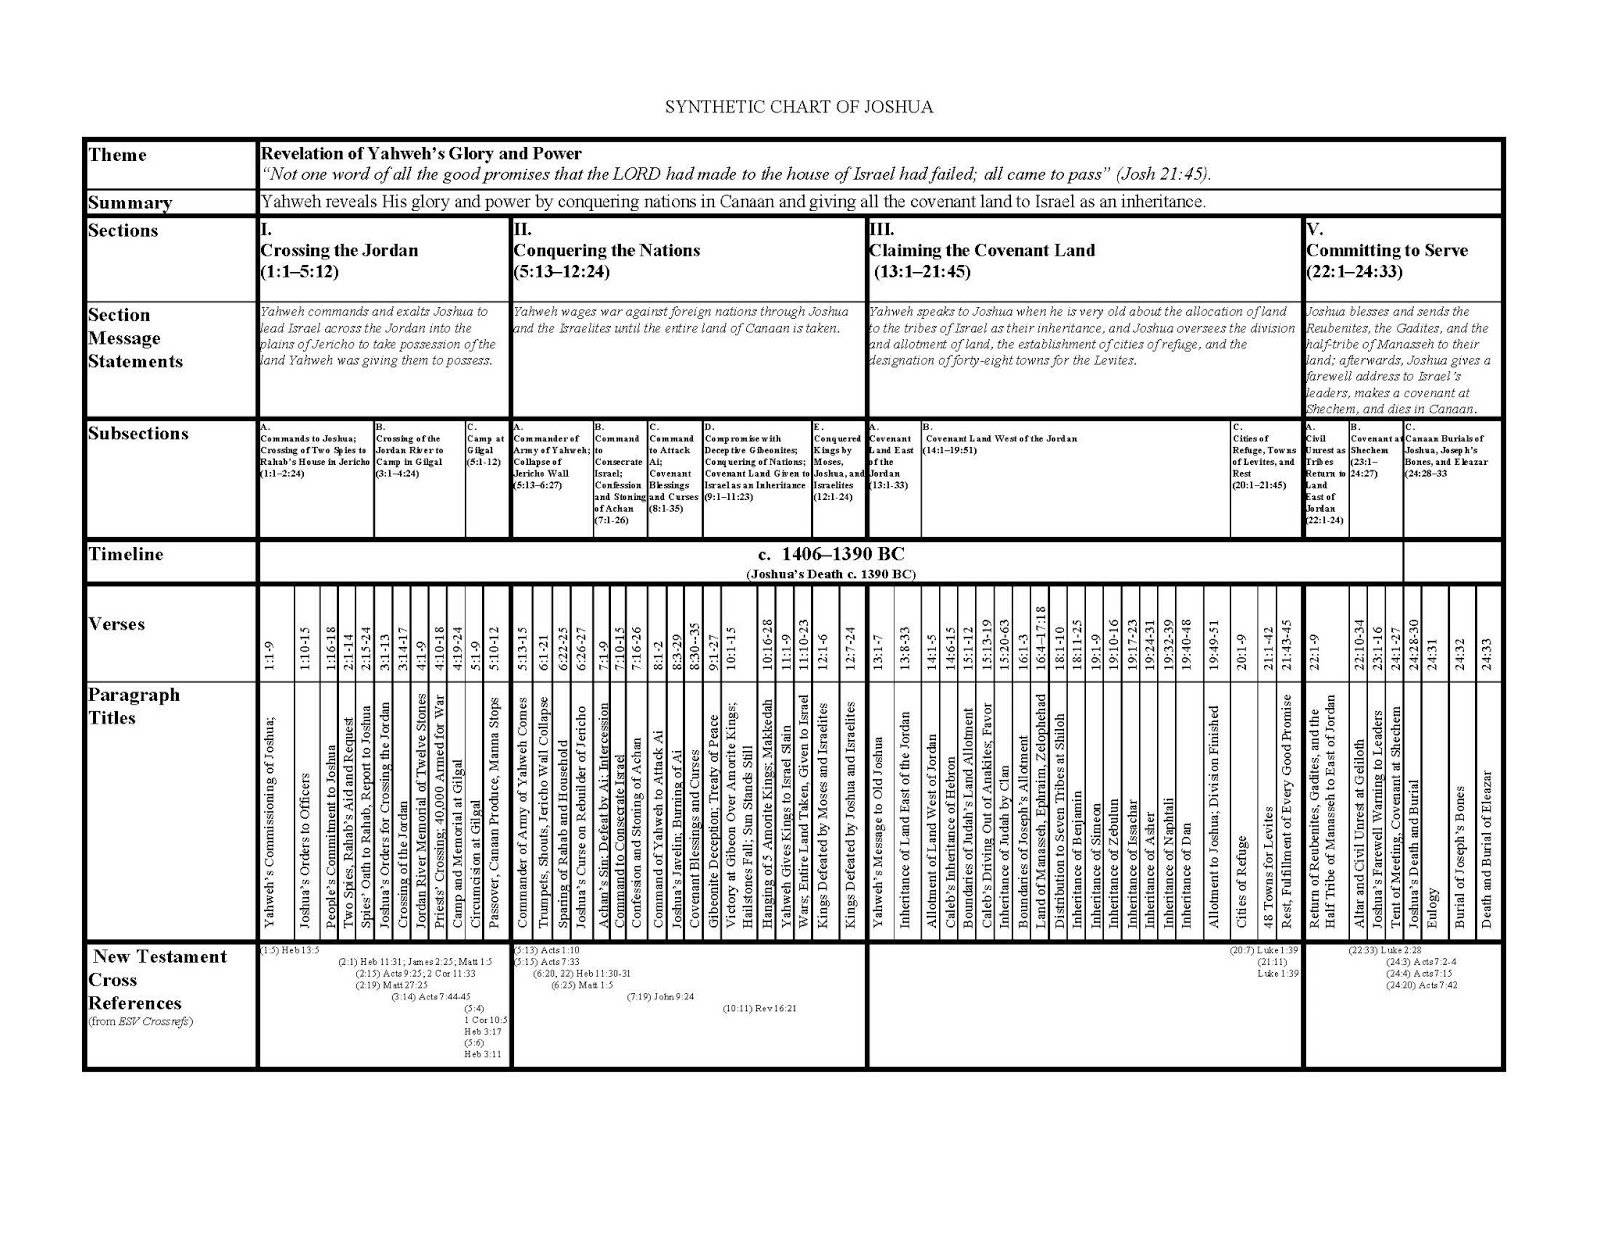
\includegraphics[scale=.4, angle=90]{06OT-Joshua/References/6.SyntheticChartofJoshua.jpg}
\caption[Synthetic Chart of Joshua]{Synthetic Chart of Joshua}
\label{fig:Synthetic Chart of Joshua}
\end{center}
\end{figure}


\newpage
\begin{figure}
\begin{center}
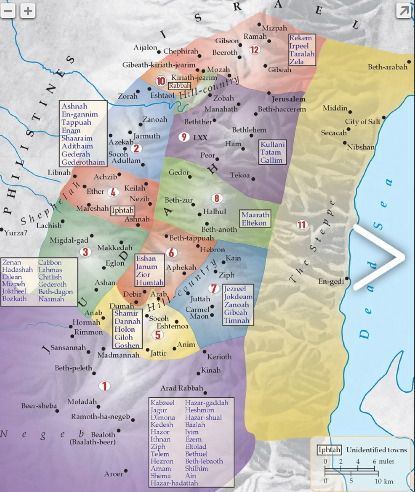
\includegraphics[scale=1, angle=0]{06OT-Joshua/References/7.WestSideOfDeadSea.jpg}
\caption[The West Side of the Dead Sea]{The West Side of the Dead Sea}
\label{fig:The West Side of the Dead Sea}
\end{center}
\end{figure}


\newpage
\begin{figure}
\begin{center}
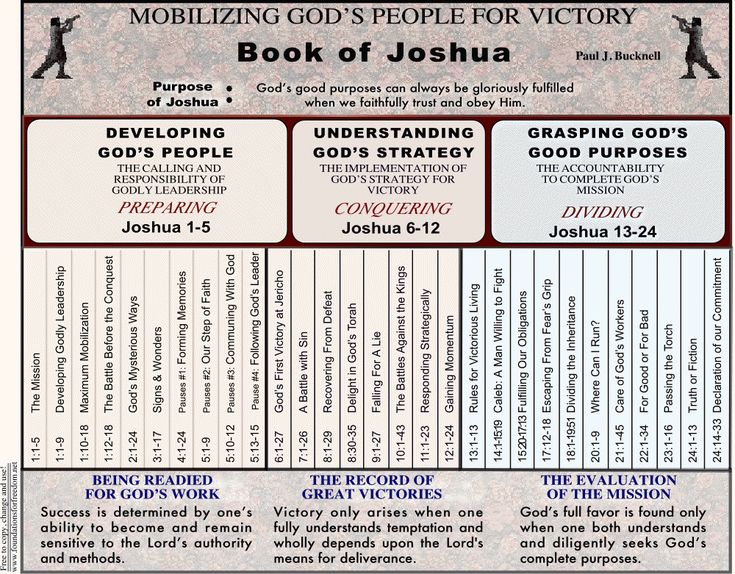
\includegraphics[scale=0.75, angle=90]{06OT-Joshua/References/8.Bucknell-Joshua.jpg}
\caption[Joshua from Bucknell]{Joshua from Bucknell}
\label{fig:Joshua from Bucknell}
\end{center}
\end{figure}


\newpage
\begin{figure}
\begin{center}
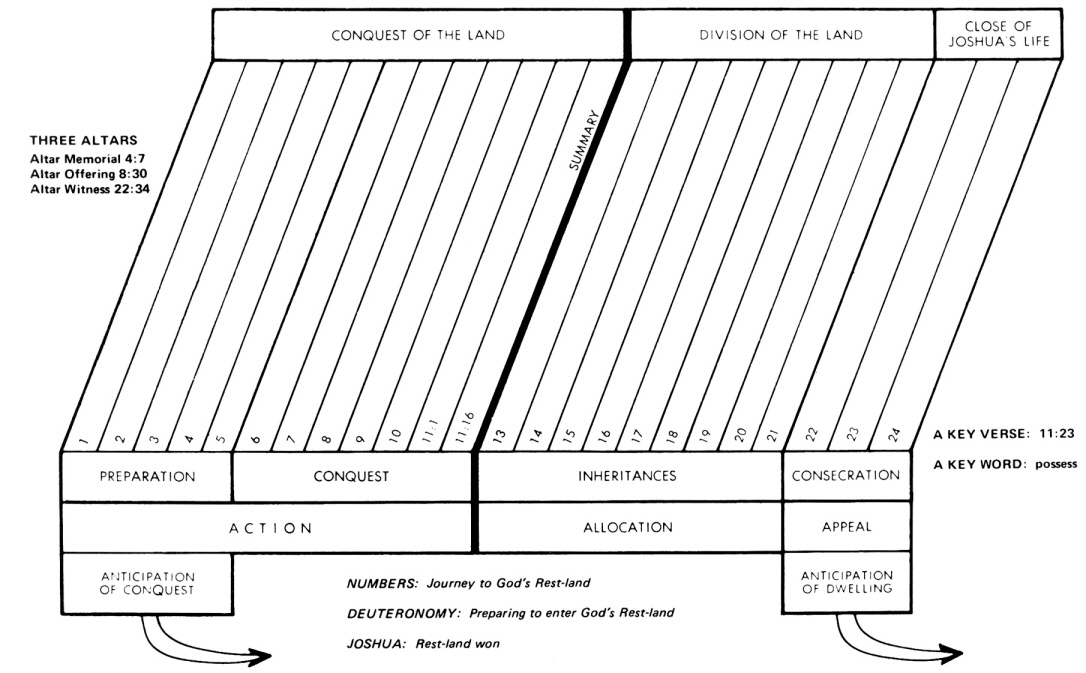
\includegraphics[scale=2, angle=90]{06OT-Joshua/References/9.Jensen-Joshua.png}
\caption[Joshua from Jensen]{Joshua from Jensen}
\label{fig:Joshua from Jensen}
\end{center}
\end{figure}


\newpage
\begin{figure}
\begin{center}
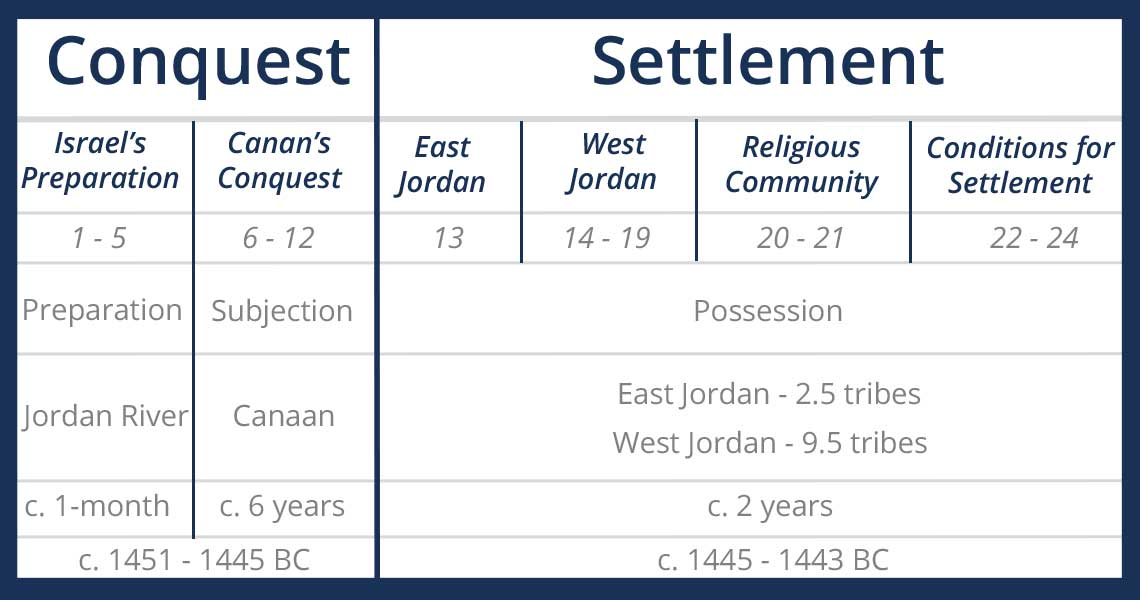
\includegraphics[scale=.5, angle=90]{06OT-Joshua/References/10.Bible-Brief-Joshua.jpg}
\caption[Bible Brief for Joshua]{Bible Brief for Joshua}
\label{fig:Bible Brief for Joshua}
\end{center}
\end{figure}

\newpage
\begin{figure}
\begin{center}
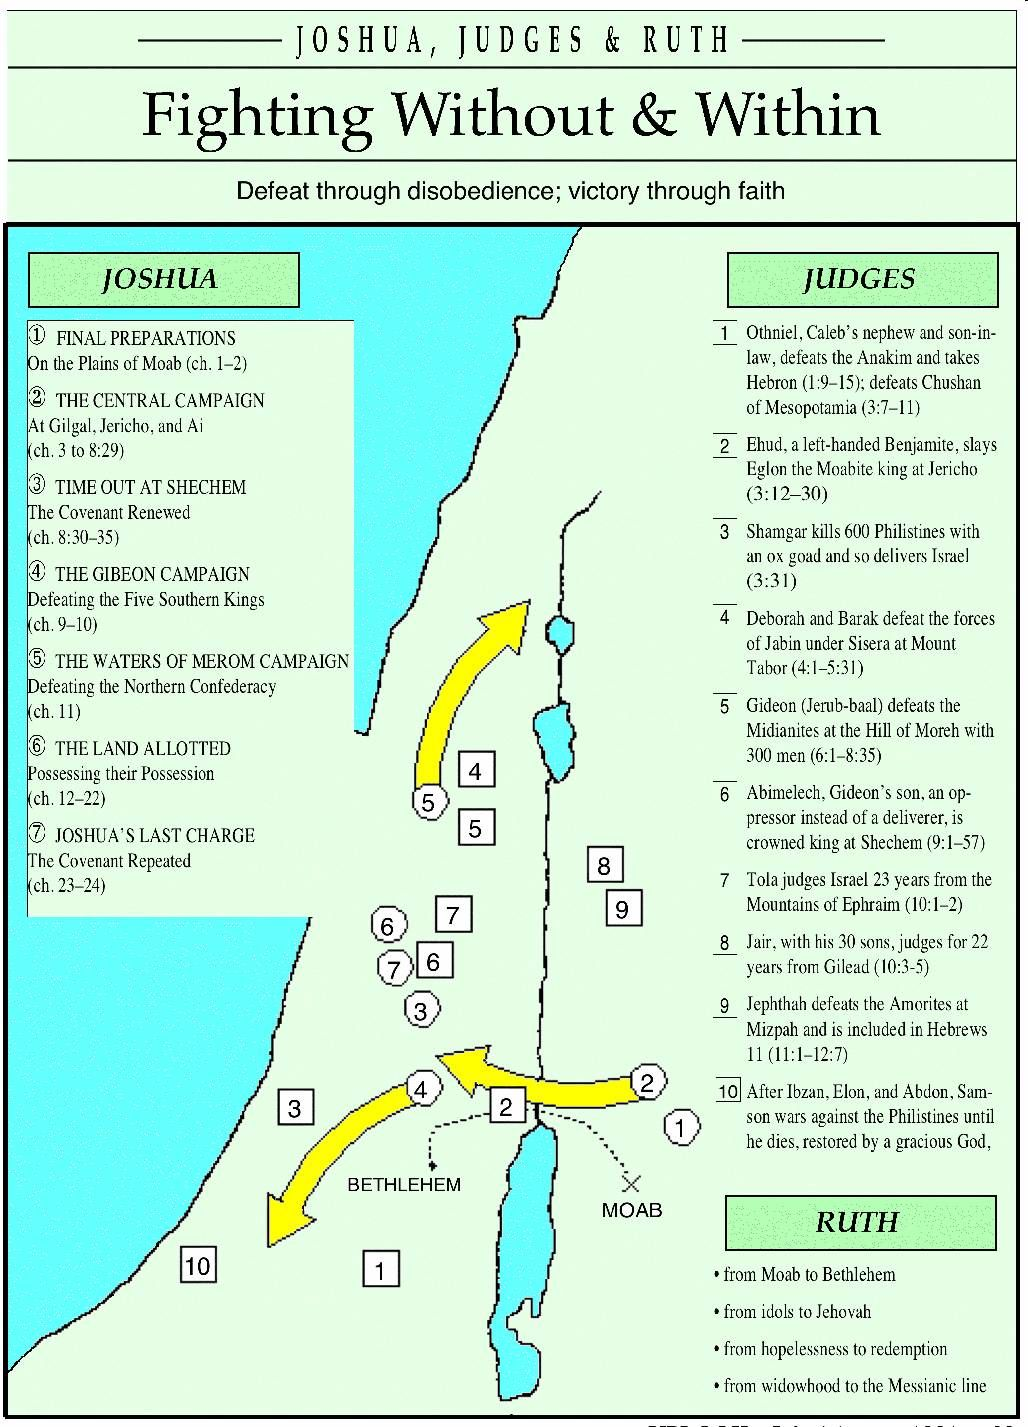
\includegraphics[scale=.5, angle=0]{06OT-Joshua/References/11.FightingInJoshuaAndJudges.jpg}
\caption[The Fighting in Joshua and Judges]{The Fighting in Joshua and Judges}
\label{fig:The Fighting in Joshua and Judges}
\end{center}
\end{figure}

\newpage
\begin{figure}
\begin{center}
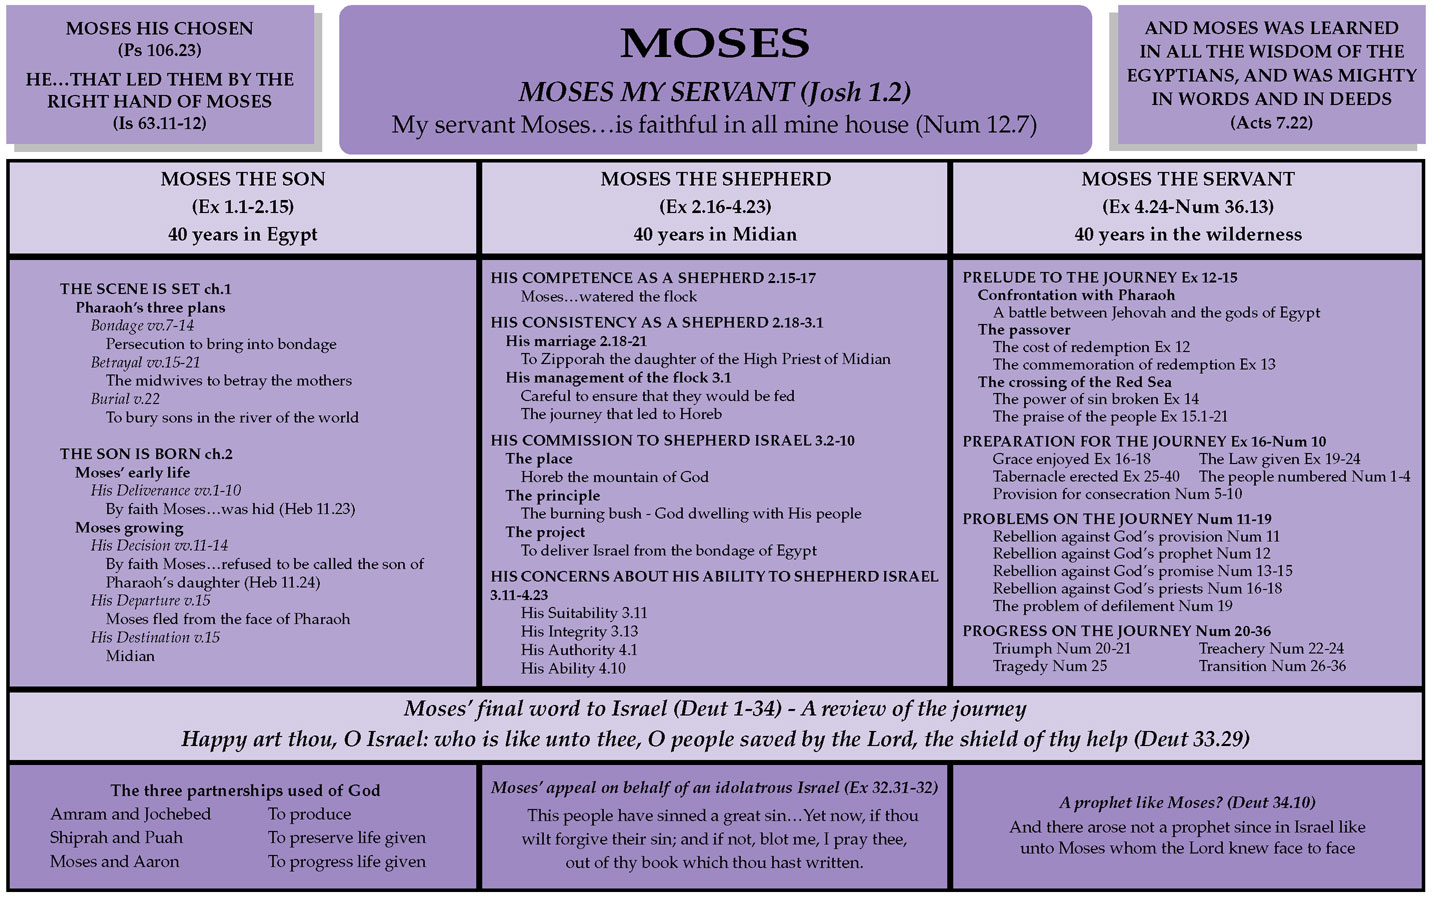
\includegraphics[scale=.4, angle=90]{06OT-Joshua/References/12.JohnGrantMoses.jpg}
\caption[Moses from John Grant]{Moses from John Grant}
\label{fig:Moses from John Grant}
\end{center}
\end{figure}







\chapter{Joshua 19}

\begin{figure}
  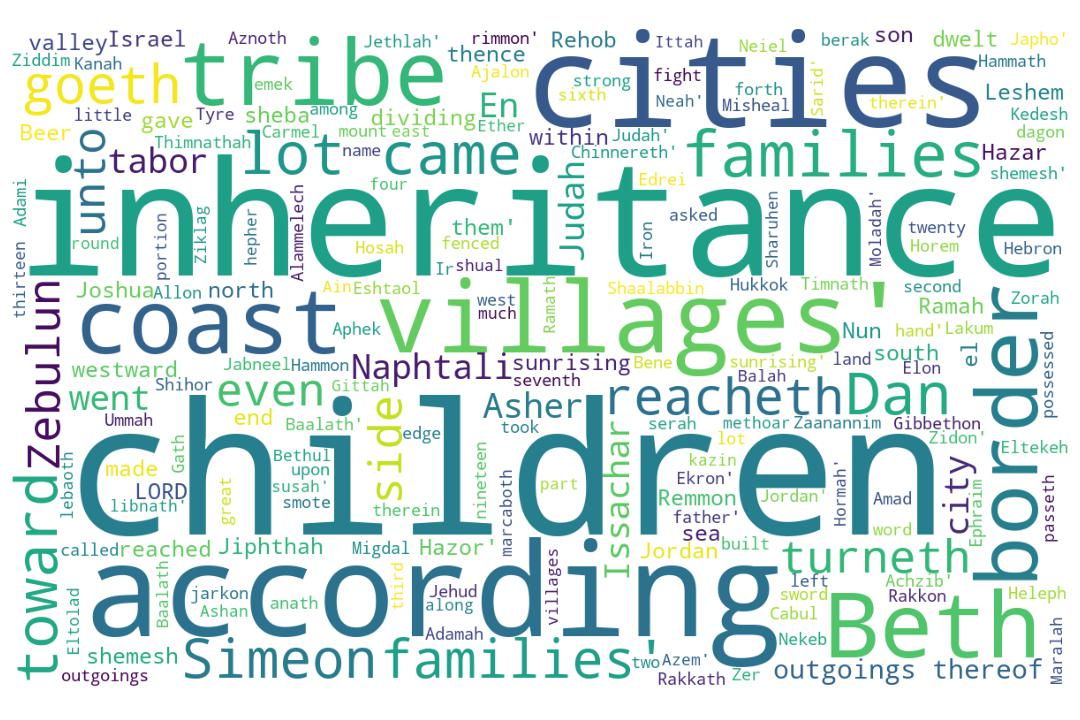
\includegraphics[width=\linewidth]{06OT-Joshua/Joshua19-WordCloud.jpg}
  \caption{Joshua 19 Word Cloud}
  \label{fig:Joshua 19 Word Cloud}
\end{figure}

\marginpar{\scriptsize \centering \fcolorbox{bone}{lime}{\textbf{SIMEON'S PORTION}}\\ (Joshua 19)

\begin{compactenum}[I.][8]

    \item \textbf{Condemned} by Jacob \index[scripture]{Genesis!Gen 34:24--30}(Gen 34:24--30)
    \item \textbf{Cut} out by Moses \index[scripture]{Deuteronomy!Deu 33:08}(Deu 33:8)
    \item To be \textbf{Cast} among Brethren \index[scripture]{Genesis!Gern 49:07}(Gen 49:7)
    \item A Story of \textbf{Carnality} %\index[scripture]{Genesis!Genesis 49:07}(Genesis 49:7)
    \item \textbf{Contained} within Judah \index[scripture]{Joshua!Jsh 19:01}(Jsh 19:1)
    \item A Story of \textbf{Consequences} \index[scripture]{Numbers!Num 25:14}(Num 25:14)

\end{compactenum}}





\footnote{\textcolor[rgb]{0.00,0.25,0.00}{\hyperlink{TOC}{Return to end of Table of Contents.}}}\footnote{\href{https://audiobible.com/bible/joshua_19.html}{\textcolor[cmyk]{0.99998,1,0,0}{Joshua 19 Audio}}}\textcolor[cmyk]{0.99998,1,0,0}{And the second lot came forth to Simeon, \emph{even} for the tribe of the children of Simeon according to their families: and their inheritance was within the inheritance of the children of Judah.}
[2] \textcolor[cmyk]{0.99998,1,0,0}{And they had in their inheritance Beer-sheba, or Sheba, and Moladah,}
[3] \textcolor[cmyk]{0.99998,1,0,0}{And Hazar-shual, and Balah, and Azem,}
[4] \textcolor[cmyk]{0.99998,1,0,0}{And Eltolad, and Bethul, and Hormah,}
[5] \textcolor[cmyk]{0.99998,1,0,0}{And Ziklag, and Beth-marcaboth, and Hazar-susah,}
[6] \textcolor[cmyk]{0.99998,1,0,0}{And Beth-lebaoth, and Sharuhen; thirteen \fcolorbox{bone}{bone}{cities} and their villages:}
[7] \textcolor[cmyk]{0.99998,1,0,0}{Ain, Remmon, and Ether, and Ashan; four \fcolorbox{bone}{bone}{cities} and their villages:}
[8] \textcolor[cmyk]{0.99998,1,0,0}{And all the villages that \emph{were} round about these \fcolorbox{bone}{bone}{cities} to Baalath-beer, Ramath of the south. This \emph{is} the inheritance of the tribe of the children of Simeon according to their families.}
[9] \textcolor[cmyk]{0.99998,1,0,0}{Out of the portion of the children of Judah \emph{was} the inheritance of the children of Simeon: for the part of the children of Judah was too much for them: therefore the children of Simeon had their inheritance within the inheritance of them.}\\
\\
\P \textcolor[cmyk]{0.99998,1,0,0}{And the third lot came up for the children of Zebulun according to their families: and the border of their inheritance was unto Sarid:}
[11] \textcolor[cmyk]{0.99998,1,0,0}{And their border went up toward the sea, and Maralah, and reached to Dabbasheth, and reached to the river that \emph{is} before Jokneam;}
[12] \textcolor[cmyk]{0.99998,1,0,0}{And turned from Sarid eastward toward the sunrising unto the border of Chisloth-tabor, and then goeth out to Daberath, and goeth up to Japhia,}
[13] \textcolor[cmyk]{0.99998,1,0,0}{And from thence passeth on along on the east to Gittah-hepher, to Ittah-kazin, and goeth out to Remmon-methoar to Neah;}
[14] \textcolor[cmyk]{0.99998,1,0,0}{And the border compasseth it on the north side to Hannathon: and the outgoings thereof are in the valley of Jiphthah-el:}
[15] \textcolor[cmyk]{0.99998,1,0,0}{And Kattath, and Nahallal, and Shimron, and Idalah, and Beth-lehem: twelve \fcolorbox{bone}{bone}{cities} with their villages.}
[16] \textcolor[cmyk]{0.99998,1,0,0}{This \emph{is} the inheritance of the children of Zebulun according to their families, these \fcolorbox{bone}{bone}{cities} with their villages.}\\
\\
\P \textcolor[cmyk]{0.99998,1,0,0}{\emph{And} the fourth lot came out to Issachar, for the children of Issachar according to their families.}
[18] \textcolor[cmyk]{0.99998,1,0,0}{And their border was toward Jezreel, and Chesulloth, and Shunem,}
[19] \textcolor[cmyk]{0.99998,1,0,0}{And Haphraim, and Shion, and Anaharath,}
[20] \textcolor[cmyk]{0.99998,1,0,0}{And Rabbith, and Kishion, and Abez,}
[21] \textcolor[cmyk]{0.99998,1,0,0}{And Remeth, and En-gannim, and En-haddah, and Beth-pazzez;}
[22] \textcolor[cmyk]{0.99998,1,0,0}{And the coast reacheth to Tabor, and Shahazimah, and Beth-shemesh; and the outgoings of their border were at Jordan: sixteen \fcolorbox{bone}{bone}{cities} with their villages.}
[23] \textcolor[cmyk]{0.99998,1,0,0}{This \emph{is} the inheritance of the tribe of the children of Issachar according to their families, the \fcolorbox{bone}{bone}{cities} and their villages.}\\
\\
\P \textcolor[cmyk]{0.99998,1,0,0}{And the fifth lot came out for the tribe of the children of Asher according to their families.}
[25] \textcolor[cmyk]{0.99998,1,0,0}{And their border was Helkath, and Hali, and Beten, and Achshaph,}[26] \textcolor[cmyk]{0.99998,1,0,0}{And Alammelech, and Amad, and Misheal; and reacheth to Carmel westward, and to Shihor-libnath;}
[27] \textcolor[cmyk]{0.99998,1,0,0}{And turneth toward the sunrising to Beth-dagon, and reacheth to Zebulun, and to the valley of Jiphthah-el toward the north side of Beth-emek, and Neiel, and goeth out to Cabul on the left hand,}
[28] \textcolor[cmyk]{0.99998,1,0,0}{And Hebron, and Rehob, and Hammon, and Kanah, \emph{even} unto great Zidon;}
[29] \textcolor[cmyk]{0.99998,1,0,0}{And \emph{then} the coast turneth to Ramah, and to the strong city Tyre; and the coast turneth to Hosah; and the outgoings thereof are at the sea from the coast to Achzib:}
[30] \textcolor[cmyk]{0.99998,1,0,0}{Ummah also, and Aphek, and Rehob: twenty and two \fcolorbox{bone}{bone}{cities} with their villages.}
[31] \textcolor[cmyk]{0.99998,1,0,0}{This \emph{is} the inheritance of the tribe of the children of Asher according to their families, these \fcolorbox{bone}{bone}{cities} with their villages.}\\
\\
\P \textcolor[cmyk]{0.99998,1,0,0}{The sixth lot came out to the children of Naphtali, \emph{even} for the children of Naphtali according to their families.}
[33] \textcolor[cmyk]{0.99998,1,0,0}{And their coast was from Heleph, from Allon to Zaanannim, and Adami, Nekeb, and Jabneel, unto Lakum; and the outgoings thereof were at Jordan:}
[34] \textcolor[cmyk]{0.99998,1,0,0}{And \emph{then} the coast turneth westward to Aznoth-tabor, and goeth out from thence to Hukkok, and reacheth to Zebulun on the south side, and reacheth to Asher on the west side, and to Judah upon Jordan toward the sunrising.}
[35] \textcolor[cmyk]{0.99998,1,0,0}{And the fenced \fcolorbox{bone}{bone}{cities} \emph{are} Ziddim, Zer, and Hammath, Rakkath, and Chinnereth,}
[36] \textcolor[cmyk]{0.99998,1,0,0}{And Adamah, and Ramah, and Hazor,}
[37] \textcolor[cmyk]{0.99998,1,0,0}{And Kedesh, and Edrei, and En-hazor,}
[38] \textcolor[cmyk]{0.99998,1,0,0}{And Iron, and Migdal-el, Horem, and Beth-anath, and Beth-shemesh; nineteen \fcolorbox{bone}{bone}{cities} with their villages.}
[39] \textcolor[cmyk]{0.99998,1,0,0}{This \emph{is} the inheritance of the tribe of the children of Naphtali according to their families, the \fcolorbox{bone}{bone}{cities} and their villages.}\\
\\
\P \textcolor[cmyk]{0.99998,1,0,0}{\emph{And} the seventh lot came out for the tribe of the children of Dan according to their families.}
[41] \textcolor[cmyk]{0.99998,1,0,0}{And the coast of their inheritance was Zorah, and Eshtaol, and Ir-shemesh,}
[42] \textcolor[cmyk]{0.99998,1,0,0}{And Shaalabbin, and Ajalon, and Jethlah,}
[43] \textcolor[cmyk]{0.99998,1,0,0}{And Elon, and Thimnathah, and Ekron,}
[44] \textcolor[cmyk]{0.99998,1,0,0}{And Eltekeh, and Gibbethon, and Baalath,}
[45] \textcolor[cmyk]{0.99998,1,0,0}{And Jehud, and Bene-berak, and Gath-rimmon,}
[46] \textcolor[cmyk]{0.99998,1,0,0}{And Me-jarkon, and Rakkon, with the border before Japho.}
[47] \textcolor[cmyk]{0.99998,1,0,0}{And the coast of the children of Dan went out \emph{too} \emph{little} for them: therefore the children of Dan went up to fight against Leshem, and took it, and smote it with the edge of the sword, and possessed it, and dwelt therein, and called Leshem, Dan, after the name of Dan their father.}
[48] \textcolor[cmyk]{0.99998,1,0,0}{This \emph{is} the inheritance of the tribe of the children of Dan according to their families, these \fcolorbox{bone}{bone}{cities} with their villages.}\\
\\
\P \textcolor[cmyk]{0.99998,1,0,0}{When they had made an end of dividing the land for inheritance by their coasts, the children of Israel gave an inheritance to Joshua the son of Nun among them:}
[50] \textcolor[cmyk]{0.99998,1,0,0}{According to the word of the LORD they gave him the city which he asked, \emph{even} Timnath-serah in mount Ephraim: and he built the city, and dwelt therein.}
[51] \textcolor[cmyk]{0.99998,1,0,0}{These \emph{are} the inheritances, which Eleazar the priest, and Joshua the son of Nun, and the heads of the fathers of the tribes of the children of Israel, divided for an inheritance by lot in Shiloh before the LORD, at the door of the tabernacle of the congregation. So they made an end of dividing the country.}
\index[NWIV]{33!Joshua!Jos 19:1}\index[AWIP]{And!Joshua!Jos 19:1}\index[AWIP]{the!Joshua!Jos 19:1}\index[AWIP]{the!Joshua!Jos 19:1 (2)}\index[AWIP]{the!Joshua!Jos 19:1 (3)}\index[AWIP]{the!Joshua!Jos 19:1 (4)}\index[AWIP]{the!Joshua!Jos 19:1 (5)}\index[AWIP]{second!Joshua!Jos 19:1}\index[AWIP]{lot!Joshua!Jos 19:1}\index[AWIP]{came!Joshua!Jos 19:1}\index[AWIP]{forth!Joshua!Jos 19:1}\index[AWIP]{to!Joshua!Jos 19:1}\index[AWIP]{to!Joshua!Jos 19:1 (2)}\index[AWIP]{Simeon!Joshua!Jos 19:1}\index[AWIP]{Simeon!Joshua!Jos 19:1 (2)}\index[AWIP]{\emph{even}!Joshua!Jos 19:1}\index[AWIP]{for!Joshua!Jos 19:1}\index[AWIP]{tribe!Joshua!Jos 19:1}\index[AWIP]{of!Joshua!Jos 19:1}\index[AWIP]{of!Joshua!Jos 19:1 (2)}\index[AWIP]{of!Joshua!Jos 19:1 (3)}\index[AWIP]{of!Joshua!Jos 19:1 (4)}\index[AWIP]{children!Joshua!Jos 19:1}\index[AWIP]{children!Joshua!Jos 19:1 (2)}\index[AWIP]{according!Joshua!Jos 19:1}\index[AWIP]{their!Joshua!Jos 19:1}\index[AWIP]{their!Joshua!Jos 19:1 (2)}\index[AWIP]{families!Joshua!Jos 19:1}\index[AWIP]{and!Joshua!Jos 19:1}\index[AWIP]{inheritance!Joshua!Jos 19:1}\index[AWIP]{inheritance!Joshua!Jos 19:1 (2)}\index[AWIP]{was!Joshua!Jos 19:1}\index[AWIP]{within!Joshua!Jos 19:1}\index[AWIP]{Judah!Joshua!Jos 19:1}\index[AWIP]{\emph{even}!Joshua!Jos 19:1}

\index[NWIV]{11!Joshua!Jos 19:2}\index[AWIP]{And!Joshua!Jos 19:2}\index[AWIP]{they!Joshua!Jos 19:2}\index[AWIP]{had!Joshua!Jos 19:2}\index[AWIP]{in!Joshua!Jos 19:2}\index[AWIP]{their!Joshua!Jos 19:2}\index[AWIP]{inheritance!Joshua!Jos 19:2}\index[AWIP]{Beer-sheba!Joshua!Jos 19:2}\index[AWIP]{or!Joshua!Jos 19:2}\index[AWIP]{Sheba!Joshua!Jos 19:2}\index[AWIP]{and!Joshua!Jos 19:2}\index[AWIP]{Moladah!Joshua!Jos 19:2}

\index[NWIV]{6!Joshua!Jos 19:3}\index[AWIP]{And!Joshua!Jos 19:3}\index[AWIP]{Hazar-shual!Joshua!Jos 19:3}\index[AWIP]{and!Joshua!Jos 19:3}\index[AWIP]{and!Joshua!Jos 19:3 (2)}\index[AWIP]{Balah!Joshua!Jos 19:3}\index[AWIP]{Azem!Joshua!Jos 19:3}

\index[NWIV]{6!Joshua!Jos 19:4}\index[AWIP]{And!Joshua!Jos 19:4}\index[AWIP]{Eltolad!Joshua!Jos 19:4}\index[AWIP]{and!Joshua!Jos 19:4}\index[AWIP]{and!Joshua!Jos 19:4 (2)}\index[AWIP]{Bethul!Joshua!Jos 19:4}\index[AWIP]{Hormah!Joshua!Jos 19:4}

\index[NWIV]{6!Joshua!Jos 19:5}\index[AWIP]{And!Joshua!Jos 19:5}\index[AWIP]{Ziklag!Joshua!Jos 19:5}\index[AWIP]{and!Joshua!Jos 19:5}\index[AWIP]{and!Joshua!Jos 19:5 (2)}\index[AWIP]{Beth-marcaboth!Joshua!Jos 19:5}\index[AWIP]{Hazar-susah!Joshua!Jos 19:5}

\index[NWIV]{9!Joshua!Jos 19:6}\index[AWIP]{And!Joshua!Jos 19:6}\index[AWIP]{Beth-lebaoth!Joshua!Jos 19:6}\index[AWIP]{and!Joshua!Jos 19:6}\index[AWIP]{and!Joshua!Jos 19:6 (2)}\index[AWIP]{Sharuhen!Joshua!Jos 19:6}\index[AWIP]{thirteen!Joshua!Jos 19:6}\index[AWIP]{cities!Joshua!Jos 19:6}\index[AWIP]{their!Joshua!Jos 19:6}\index[AWIP]{villages!Joshua!Jos 19:6}

\index[NWIV]{11!Joshua!Jos 19:7}\index[AWIP]{Ain!Joshua!Jos 19:7}\index[AWIP]{Remmon!Joshua!Jos 19:7}\index[AWIP]{and!Joshua!Jos 19:7}\index[AWIP]{and!Joshua!Jos 19:7 (2)}\index[AWIP]{and!Joshua!Jos 19:7 (3)}\index[AWIP]{Ether!Joshua!Jos 19:7}\index[AWIP]{Ashan!Joshua!Jos 19:7}\index[AWIP]{four!Joshua!Jos 19:7}\index[AWIP]{cities!Joshua!Jos 19:7}\index[AWIP]{their!Joshua!Jos 19:7}\index[AWIP]{villages!Joshua!Jos 19:7}

\index[NWIV]{32!Joshua!Jos 19:8}\index[AWIP]{And!Joshua!Jos 19:8}\index[AWIP]{all!Joshua!Jos 19:8}\index[AWIP]{the!Joshua!Jos 19:8}\index[AWIP]{the!Joshua!Jos 19:8 (2)}\index[AWIP]{the!Joshua!Jos 19:8 (3)}\index[AWIP]{the!Joshua!Jos 19:8 (4)}\index[AWIP]{the!Joshua!Jos 19:8 (5)}\index[AWIP]{villages!Joshua!Jos 19:8}\index[AWIP]{that!Joshua!Jos 19:8}\index[AWIP]{\emph{were}!Joshua!Jos 19:8}\index[AWIP]{round!Joshua!Jos 19:8}\index[AWIP]{about!Joshua!Jos 19:8}\index[AWIP]{these!Joshua!Jos 19:8}\index[AWIP]{cities!Joshua!Jos 19:8}\index[AWIP]{to!Joshua!Jos 19:8}\index[AWIP]{to!Joshua!Jos 19:8 (2)}\index[AWIP]{Baalath-beer!Joshua!Jos 19:8}\index[AWIP]{Ramath!Joshua!Jos 19:8}\index[AWIP]{of!Joshua!Jos 19:8}\index[AWIP]{of!Joshua!Jos 19:8 (2)}\index[AWIP]{of!Joshua!Jos 19:8 (3)}\index[AWIP]{of!Joshua!Jos 19:8 (4)}\index[AWIP]{south!Joshua!Jos 19:8}\index[AWIP]{This!Joshua!Jos 19:8}\index[AWIP]{\emph{is}!Joshua!Jos 19:8}\index[AWIP]{inheritance!Joshua!Jos 19:8}\index[AWIP]{tribe!Joshua!Jos 19:8}\index[AWIP]{children!Joshua!Jos 19:8}\index[AWIP]{Simeon!Joshua!Jos 19:8}\index[AWIP]{according!Joshua!Jos 19:8}\index[AWIP]{their!Joshua!Jos 19:8}\index[AWIP]{families!Joshua!Jos 19:8}\index[AWIP]{\emph{were}!Joshua!Jos 19:8}\index[AWIP]{\emph{is}!Joshua!Jos 19:8}

\index[NWIV]{43!Joshua!Jos 19:9}\index[AWIP]{Out!Joshua!Jos 19:9}\index[AWIP]{of!Joshua!Jos 19:9}\index[AWIP]{of!Joshua!Jos 19:9 (2)}\index[AWIP]{of!Joshua!Jos 19:9 (3)}\index[AWIP]{of!Joshua!Jos 19:9 (4)}\index[AWIP]{of!Joshua!Jos 19:9 (5)}\index[AWIP]{of!Joshua!Jos 19:9 (6)}\index[AWIP]{of!Joshua!Jos 19:9 (7)}\index[AWIP]{of!Joshua!Jos 19:9 (8)}\index[AWIP]{of!Joshua!Jos 19:9 (9)}\index[AWIP]{the!Joshua!Jos 19:9}\index[AWIP]{the!Joshua!Jos 19:9 (2)}\index[AWIP]{the!Joshua!Jos 19:9 (3)}\index[AWIP]{the!Joshua!Jos 19:9 (4)}\index[AWIP]{the!Joshua!Jos 19:9 (5)}\index[AWIP]{the!Joshua!Jos 19:9 (6)}\index[AWIP]{the!Joshua!Jos 19:9 (7)}\index[AWIP]{the!Joshua!Jos 19:9 (8)}\index[AWIP]{portion!Joshua!Jos 19:9}\index[AWIP]{children!Joshua!Jos 19:9}\index[AWIP]{children!Joshua!Jos 19:9 (2)}\index[AWIP]{children!Joshua!Jos 19:9 (3)}\index[AWIP]{children!Joshua!Jos 19:9 (4)}\index[AWIP]{Judah!Joshua!Jos 19:9}\index[AWIP]{Judah!Joshua!Jos 19:9 (2)}\index[AWIP]{\emph{was}!Joshua!Jos 19:9}\index[AWIP]{inheritance!Joshua!Jos 19:9}\index[AWIP]{inheritance!Joshua!Jos 19:9 (2)}\index[AWIP]{inheritance!Joshua!Jos 19:9 (3)}\index[AWIP]{Simeon!Joshua!Jos 19:9}\index[AWIP]{Simeon!Joshua!Jos 19:9 (2)}\index[AWIP]{for!Joshua!Jos 19:9}\index[AWIP]{for!Joshua!Jos 19:9 (2)}\index[AWIP]{part!Joshua!Jos 19:9}\index[AWIP]{was!Joshua!Jos 19:9}\index[AWIP]{too!Joshua!Jos 19:9}\index[AWIP]{much!Joshua!Jos 19:9}\index[AWIP]{them!Joshua!Jos 19:9}\index[AWIP]{them!Joshua!Jos 19:9 (2)}\index[AWIP]{therefore!Joshua!Jos 19:9}\index[AWIP]{had!Joshua!Jos 19:9}\index[AWIP]{their!Joshua!Jos 19:9}\index[AWIP]{within!Joshua!Jos 19:9}\index[AWIP]{\emph{was}!Joshua!Jos 19:9}

\index[NWIV]{24!Joshua!Jos 19:10}\index[AWIP]{And!Joshua!Jos 19:10}\index[AWIP]{the!Joshua!Jos 19:10}\index[AWIP]{the!Joshua!Jos 19:10 (2)}\index[AWIP]{the!Joshua!Jos 19:10 (3)}\index[AWIP]{third!Joshua!Jos 19:10}\index[AWIP]{lot!Joshua!Jos 19:10}\index[AWIP]{came!Joshua!Jos 19:10}\index[AWIP]{up!Joshua!Jos 19:10}\index[AWIP]{for!Joshua!Jos 19:10}\index[AWIP]{children!Joshua!Jos 19:10}\index[AWIP]{of!Joshua!Jos 19:10}\index[AWIP]{of!Joshua!Jos 19:10 (2)}\index[AWIP]{Zebulun!Joshua!Jos 19:10}\index[AWIP]{according!Joshua!Jos 19:10}\index[AWIP]{to!Joshua!Jos 19:10}\index[AWIP]{their!Joshua!Jos 19:10}\index[AWIP]{their!Joshua!Jos 19:10 (2)}\index[AWIP]{families!Joshua!Jos 19:10}\index[AWIP]{and!Joshua!Jos 19:10}\index[AWIP]{border!Joshua!Jos 19:10}\index[AWIP]{inheritance!Joshua!Jos 19:10}\index[AWIP]{was!Joshua!Jos 19:10}\index[AWIP]{unto!Joshua!Jos 19:10}\index[AWIP]{Sarid!Joshua!Jos 19:10}

\index[NWIV]{23!Joshua!Jos 19:11}\index[AWIP]{And!Joshua!Jos 19:11}\index[AWIP]{their!Joshua!Jos 19:11}\index[AWIP]{border!Joshua!Jos 19:11}\index[AWIP]{went!Joshua!Jos 19:11}\index[AWIP]{up!Joshua!Jos 19:11}\index[AWIP]{toward!Joshua!Jos 19:11}\index[AWIP]{the!Joshua!Jos 19:11}\index[AWIP]{the!Joshua!Jos 19:11 (2)}\index[AWIP]{sea!Joshua!Jos 19:11}\index[AWIP]{and!Joshua!Jos 19:11}\index[AWIP]{and!Joshua!Jos 19:11 (2)}\index[AWIP]{and!Joshua!Jos 19:11 (3)}\index[AWIP]{Maralah!Joshua!Jos 19:11}\index[AWIP]{reached!Joshua!Jos 19:11}\index[AWIP]{reached!Joshua!Jos 19:11 (2)}\index[AWIP]{to!Joshua!Jos 19:11}\index[AWIP]{to!Joshua!Jos 19:11 (2)}\index[AWIP]{Dabbasheth!Joshua!Jos 19:11}\index[AWIP]{river!Joshua!Jos 19:11}\index[AWIP]{that!Joshua!Jos 19:11}\index[AWIP]{\emph{is}!Joshua!Jos 19:11}\index[AWIP]{before!Joshua!Jos 19:11}\index[AWIP]{Jokneam!Joshua!Jos 19:11}\index[AWIP]{\emph{is}!Joshua!Jos 19:11}

\index[NWIV]{24!Joshua!Jos 19:12}\index[AWIP]{And!Joshua!Jos 19:12}\index[AWIP]{turned!Joshua!Jos 19:12}\index[AWIP]{from!Joshua!Jos 19:12}\index[AWIP]{Sarid!Joshua!Jos 19:12}\index[AWIP]{eastward!Joshua!Jos 19:12}\index[AWIP]{toward!Joshua!Jos 19:12}\index[AWIP]{the!Joshua!Jos 19:12}\index[AWIP]{the!Joshua!Jos 19:12 (2)}\index[AWIP]{sunrising!Joshua!Jos 19:12}\index[AWIP]{unto!Joshua!Jos 19:12}\index[AWIP]{border!Joshua!Jos 19:12}\index[AWIP]{of!Joshua!Jos 19:12}\index[AWIP]{Chisloth-tabor!Joshua!Jos 19:12}\index[AWIP]{and!Joshua!Jos 19:12}\index[AWIP]{and!Joshua!Jos 19:12 (2)}\index[AWIP]{then!Joshua!Jos 19:12}\index[AWIP]{goeth!Joshua!Jos 19:12}\index[AWIP]{goeth!Joshua!Jos 19:12 (2)}\index[AWIP]{out!Joshua!Jos 19:12}\index[AWIP]{to!Joshua!Jos 19:12}\index[AWIP]{to!Joshua!Jos 19:12 (2)}\index[AWIP]{Daberath!Joshua!Jos 19:12}\index[AWIP]{up!Joshua!Jos 19:12}\index[AWIP]{Japhia!Joshua!Jos 19:12}

\index[NWIV]{20!Joshua!Jos 19:13}\index[AWIP]{And!Joshua!Jos 19:13}\index[AWIP]{from!Joshua!Jos 19:13}\index[AWIP]{thence!Joshua!Jos 19:13}\index[AWIP]{passeth!Joshua!Jos 19:13}\index[AWIP]{on!Joshua!Jos 19:13}\index[AWIP]{on!Joshua!Jos 19:13 (2)}\index[AWIP]{along!Joshua!Jos 19:13}\index[AWIP]{the!Joshua!Jos 19:13}\index[AWIP]{east!Joshua!Jos 19:13}\index[AWIP]{to!Joshua!Jos 19:13}\index[AWIP]{to!Joshua!Jos 19:13 (2)}\index[AWIP]{to!Joshua!Jos 19:13 (3)}\index[AWIP]{to!Joshua!Jos 19:13 (4)}\index[AWIP]{Gittah-hepher!Joshua!Jos 19:13}\index[AWIP]{Ittah-kazin!Joshua!Jos 19:13}\index[AWIP]{and!Joshua!Jos 19:13}\index[AWIP]{goeth!Joshua!Jos 19:13}\index[AWIP]{out!Joshua!Jos 19:13}\index[AWIP]{Remmon-methoar!Joshua!Jos 19:13}\index[AWIP]{Neah!Joshua!Jos 19:13}

\index[NWIV]{21!Joshua!Jos 19:14}\index[AWIP]{And!Joshua!Jos 19:14}\index[AWIP]{the!Joshua!Jos 19:14}\index[AWIP]{the!Joshua!Jos 19:14 (2)}\index[AWIP]{the!Joshua!Jos 19:14 (3)}\index[AWIP]{the!Joshua!Jos 19:14 (4)}\index[AWIP]{border!Joshua!Jos 19:14}\index[AWIP]{compasseth!Joshua!Jos 19:14}\index[AWIP]{it!Joshua!Jos 19:14}\index[AWIP]{on!Joshua!Jos 19:14}\index[AWIP]{north!Joshua!Jos 19:14}\index[AWIP]{side!Joshua!Jos 19:14}\index[AWIP]{to!Joshua!Jos 19:14}\index[AWIP]{Hannathon!Joshua!Jos 19:14}\index[AWIP]{and!Joshua!Jos 19:14}\index[AWIP]{outgoings!Joshua!Jos 19:14}\index[AWIP]{thereof!Joshua!Jos 19:14}\index[AWIP]{are!Joshua!Jos 19:14}\index[AWIP]{in!Joshua!Jos 19:14}\index[AWIP]{valley!Joshua!Jos 19:14}\index[AWIP]{of!Joshua!Jos 19:14}\index[AWIP]{Jiphthah-el!Joshua!Jos 19:14}

\index[NWIV]{15!Joshua!Jos 19:15}\index[AWIP]{And!Joshua!Jos 19:15}\index[AWIP]{Kattath!Joshua!Jos 19:15}\index[AWIP]{and!Joshua!Jos 19:15}\index[AWIP]{and!Joshua!Jos 19:15 (2)}\index[AWIP]{and!Joshua!Jos 19:15 (3)}\index[AWIP]{and!Joshua!Jos 19:15 (4)}\index[AWIP]{Nahallal!Joshua!Jos 19:15}\index[AWIP]{Shimron!Joshua!Jos 19:15}\index[AWIP]{Idalah!Joshua!Jos 19:15}\index[AWIP]{Beth-lehem!Joshua!Jos 19:15}\index[AWIP]{twelve!Joshua!Jos 19:15}\index[AWIP]{cities!Joshua!Jos 19:15}\index[AWIP]{with!Joshua!Jos 19:15}\index[AWIP]{their!Joshua!Jos 19:15}\index[AWIP]{villages!Joshua!Jos 19:15}

\index[NWIV]{18!Joshua!Jos 19:16}\index[AWIP]{This!Joshua!Jos 19:16}\index[AWIP]{\emph{is}!Joshua!Jos 19:16}\index[AWIP]{the!Joshua!Jos 19:16}\index[AWIP]{the!Joshua!Jos 19:16 (2)}\index[AWIP]{inheritance!Joshua!Jos 19:16}\index[AWIP]{of!Joshua!Jos 19:16}\index[AWIP]{of!Joshua!Jos 19:16 (2)}\index[AWIP]{children!Joshua!Jos 19:16}\index[AWIP]{Zebulun!Joshua!Jos 19:16}\index[AWIP]{according!Joshua!Jos 19:16}\index[AWIP]{to!Joshua!Jos 19:16}\index[AWIP]{their!Joshua!Jos 19:16}\index[AWIP]{their!Joshua!Jos 19:16 (2)}\index[AWIP]{families!Joshua!Jos 19:16}\index[AWIP]{these!Joshua!Jos 19:16}\index[AWIP]{cities!Joshua!Jos 19:16}\index[AWIP]{with!Joshua!Jos 19:16}\index[AWIP]{villages!Joshua!Jos 19:16}\index[AWIP]{\emph{is}!Joshua!Jos 19:16}

\index[NWIV]{17!Joshua!Jos 19:17}\index[AWIP]{\emph{And}!Joshua!Jos 19:17}\index[AWIP]{the!Joshua!Jos 19:17}\index[AWIP]{the!Joshua!Jos 19:17 (2)}\index[AWIP]{fourth!Joshua!Jos 19:17}\index[AWIP]{lot!Joshua!Jos 19:17}\index[AWIP]{came!Joshua!Jos 19:17}\index[AWIP]{out!Joshua!Jos 19:17}\index[AWIP]{to!Joshua!Jos 19:17}\index[AWIP]{to!Joshua!Jos 19:17 (2)}\index[AWIP]{Issachar!Joshua!Jos 19:17}\index[AWIP]{Issachar!Joshua!Jos 19:17 (2)}\index[AWIP]{for!Joshua!Jos 19:17}\index[AWIP]{children!Joshua!Jos 19:17}\index[AWIP]{of!Joshua!Jos 19:17}\index[AWIP]{according!Joshua!Jos 19:17}\index[AWIP]{their!Joshua!Jos 19:17}\index[AWIP]{families!Joshua!Jos 19:17}\index[AWIP]{\emph{And}!Joshua!Jos 19:17}

\index[NWIV]{10!Joshua!Jos 19:18}\index[AWIP]{And!Joshua!Jos 19:18}\index[AWIP]{their!Joshua!Jos 19:18}\index[AWIP]{border!Joshua!Jos 19:18}\index[AWIP]{was!Joshua!Jos 19:18}\index[AWIP]{toward!Joshua!Jos 19:18}\index[AWIP]{Jezreel!Joshua!Jos 19:18}\index[AWIP]{and!Joshua!Jos 19:18}\index[AWIP]{and!Joshua!Jos 19:18 (2)}\index[AWIP]{Chesulloth!Joshua!Jos 19:18}\index[AWIP]{Shunem!Joshua!Jos 19:18}

\index[NWIV]{6!Joshua!Jos 19:19}\index[AWIP]{And!Joshua!Jos 19:19}\index[AWIP]{Haphraim!Joshua!Jos 19:19}\index[AWIP]{and!Joshua!Jos 19:19}\index[AWIP]{and!Joshua!Jos 19:19 (2)}\index[AWIP]{Shion!Joshua!Jos 19:19}\index[AWIP]{Anaharath!Joshua!Jos 19:19}

\index[NWIV]{6!Joshua!Jos 19:20}\index[AWIP]{And!Joshua!Jos 19:20}\index[AWIP]{Rabbith!Joshua!Jos 19:20}\index[AWIP]{and!Joshua!Jos 19:20}\index[AWIP]{and!Joshua!Jos 19:20 (2)}\index[AWIP]{Kishion!Joshua!Jos 19:20}\index[AWIP]{Abez!Joshua!Jos 19:20}

\index[NWIV]{8!Joshua!Jos 19:21}\index[AWIP]{And!Joshua!Jos 19:21}\index[AWIP]{Remeth!Joshua!Jos 19:21}\index[AWIP]{and!Joshua!Jos 19:21}\index[AWIP]{and!Joshua!Jos 19:21 (2)}\index[AWIP]{and!Joshua!Jos 19:21 (3)}\index[AWIP]{En-gannim!Joshua!Jos 19:21}\index[AWIP]{En-haddah!Joshua!Jos 19:21}\index[AWIP]{Beth-pazzez!Joshua!Jos 19:21}

\index[NWIV]{24!Joshua!Jos 19:22}\index[AWIP]{And!Joshua!Jos 19:22}\index[AWIP]{the!Joshua!Jos 19:22}\index[AWIP]{the!Joshua!Jos 19:22 (2)}\index[AWIP]{coast!Joshua!Jos 19:22}\index[AWIP]{reacheth!Joshua!Jos 19:22}\index[AWIP]{to!Joshua!Jos 19:22}\index[AWIP]{Tabor!Joshua!Jos 19:22}\index[AWIP]{and!Joshua!Jos 19:22}\index[AWIP]{and!Joshua!Jos 19:22 (2)}\index[AWIP]{and!Joshua!Jos 19:22 (3)}\index[AWIP]{Shahazimah!Joshua!Jos 19:22}\index[AWIP]{Beth-shemesh!Joshua!Jos 19:22}\index[AWIP]{outgoings!Joshua!Jos 19:22}\index[AWIP]{of!Joshua!Jos 19:22}\index[AWIP]{their!Joshua!Jos 19:22}\index[AWIP]{their!Joshua!Jos 19:22 (2)}\index[AWIP]{border!Joshua!Jos 19:22}\index[AWIP]{were!Joshua!Jos 19:22}\index[AWIP]{at!Joshua!Jos 19:22}\index[AWIP]{Jordan!Joshua!Jos 19:22}\index[AWIP]{sixteen!Joshua!Jos 19:22}\index[AWIP]{cities!Joshua!Jos 19:22}\index[AWIP]{with!Joshua!Jos 19:22}\index[AWIP]{villages!Joshua!Jos 19:22}

\index[NWIV]{21!Joshua!Jos 19:23}\index[AWIP]{This!Joshua!Jos 19:23}\index[AWIP]{\emph{is}!Joshua!Jos 19:23}\index[AWIP]{the!Joshua!Jos 19:23}\index[AWIP]{the!Joshua!Jos 19:23 (2)}\index[AWIP]{the!Joshua!Jos 19:23 (3)}\index[AWIP]{the!Joshua!Jos 19:23 (4)}\index[AWIP]{inheritance!Joshua!Jos 19:23}\index[AWIP]{of!Joshua!Jos 19:23}\index[AWIP]{of!Joshua!Jos 19:23 (2)}\index[AWIP]{of!Joshua!Jos 19:23 (3)}\index[AWIP]{tribe!Joshua!Jos 19:23}\index[AWIP]{children!Joshua!Jos 19:23}\index[AWIP]{Issachar!Joshua!Jos 19:23}\index[AWIP]{according!Joshua!Jos 19:23}\index[AWIP]{to!Joshua!Jos 19:23}\index[AWIP]{their!Joshua!Jos 19:23}\index[AWIP]{their!Joshua!Jos 19:23 (2)}\index[AWIP]{families!Joshua!Jos 19:23}\index[AWIP]{cities!Joshua!Jos 19:23}\index[AWIP]{and!Joshua!Jos 19:23}\index[AWIP]{villages!Joshua!Jos 19:23}\index[AWIP]{\emph{is}!Joshua!Jos 19:23}

\index[NWIV]{18!Joshua!Jos 19:24}\index[AWIP]{And!Joshua!Jos 19:24}\index[AWIP]{the!Joshua!Jos 19:24}\index[AWIP]{the!Joshua!Jos 19:24 (2)}\index[AWIP]{the!Joshua!Jos 19:24 (3)}\index[AWIP]{fifth!Joshua!Jos 19:24}\index[AWIP]{lot!Joshua!Jos 19:24}\index[AWIP]{came!Joshua!Jos 19:24}\index[AWIP]{out!Joshua!Jos 19:24}\index[AWIP]{for!Joshua!Jos 19:24}\index[AWIP]{tribe!Joshua!Jos 19:24}\index[AWIP]{of!Joshua!Jos 19:24}\index[AWIP]{of!Joshua!Jos 19:24 (2)}\index[AWIP]{children!Joshua!Jos 19:24}\index[AWIP]{Asher!Joshua!Jos 19:24}\index[AWIP]{according!Joshua!Jos 19:24}\index[AWIP]{to!Joshua!Jos 19:24}\index[AWIP]{their!Joshua!Jos 19:24}\index[AWIP]{families!Joshua!Jos 19:24}

\index[NWIV]{11!Joshua!Jos 19:25}\index[AWIP]{And!Joshua!Jos 19:25}\index[AWIP]{their!Joshua!Jos 19:25}\index[AWIP]{border!Joshua!Jos 19:25}\index[AWIP]{was!Joshua!Jos 19:25}\index[AWIP]{Helkath!Joshua!Jos 19:25}\index[AWIP]{and!Joshua!Jos 19:25}\index[AWIP]{and!Joshua!Jos 19:25 (2)}\index[AWIP]{and!Joshua!Jos 19:25 (3)}\index[AWIP]{Hali!Joshua!Jos 19:25}\index[AWIP]{Beten!Joshua!Jos 19:25}\index[AWIP]{Achshaph!Joshua!Jos 19:25}

\index[NWIV]{14!Joshua!Jos 19:26}\index[AWIP]{And!Joshua!Jos 19:26}\index[AWIP]{Alammelech!Joshua!Jos 19:26}\index[AWIP]{and!Joshua!Jos 19:26}\index[AWIP]{and!Joshua!Jos 19:26 (2)}\index[AWIP]{and!Joshua!Jos 19:26 (3)}\index[AWIP]{and!Joshua!Jos 19:26 (4)}\index[AWIP]{Amad!Joshua!Jos 19:26}\index[AWIP]{Misheal!Joshua!Jos 19:26}\index[AWIP]{reacheth!Joshua!Jos 19:26}\index[AWIP]{to!Joshua!Jos 19:26}\index[AWIP]{to!Joshua!Jos 19:26 (2)}\index[AWIP]{Carmel!Joshua!Jos 19:26}\index[AWIP]{westward!Joshua!Jos 19:26}\index[AWIP]{Shihor-libnath!Joshua!Jos 19:26}

\index[NWIV]{34!Joshua!Jos 19:27}\index[AWIP]{And!Joshua!Jos 19:27}\index[AWIP]{turneth!Joshua!Jos 19:27}\index[AWIP]{toward!Joshua!Jos 19:27}\index[AWIP]{toward!Joshua!Jos 19:27 (2)}\index[AWIP]{the!Joshua!Jos 19:27}\index[AWIP]{the!Joshua!Jos 19:27 (2)}\index[AWIP]{the!Joshua!Jos 19:27 (3)}\index[AWIP]{the!Joshua!Jos 19:27 (4)}\index[AWIP]{sunrising!Joshua!Jos 19:27}\index[AWIP]{to!Joshua!Jos 19:27}\index[AWIP]{to!Joshua!Jos 19:27 (2)}\index[AWIP]{to!Joshua!Jos 19:27 (3)}\index[AWIP]{to!Joshua!Jos 19:27 (4)}\index[AWIP]{Beth-dagon!Joshua!Jos 19:27}\index[AWIP]{and!Joshua!Jos 19:27}\index[AWIP]{and!Joshua!Jos 19:27 (2)}\index[AWIP]{and!Joshua!Jos 19:27 (3)}\index[AWIP]{and!Joshua!Jos 19:27 (4)}\index[AWIP]{reacheth!Joshua!Jos 19:27}\index[AWIP]{Zebulun!Joshua!Jos 19:27}\index[AWIP]{valley!Joshua!Jos 19:27}\index[AWIP]{of!Joshua!Jos 19:27}\index[AWIP]{of!Joshua!Jos 19:27 (2)}\index[AWIP]{Jiphthah-el!Joshua!Jos 19:27}\index[AWIP]{north!Joshua!Jos 19:27}\index[AWIP]{side!Joshua!Jos 19:27}\index[AWIP]{Beth-emek!Joshua!Jos 19:27}\index[AWIP]{Neiel!Joshua!Jos 19:27}\index[AWIP]{goeth!Joshua!Jos 19:27}\index[AWIP]{out!Joshua!Jos 19:27}\index[AWIP]{Cabul!Joshua!Jos 19:27}\index[AWIP]{on!Joshua!Jos 19:27}\index[AWIP]{left!Joshua!Jos 19:27}\index[AWIP]{hand!Joshua!Jos 19:27}

\index[NWIV]{12!Joshua!Jos 19:28}\index[AWIP]{And!Joshua!Jos 19:28}\index[AWIP]{Hebron!Joshua!Jos 19:28}\index[AWIP]{and!Joshua!Jos 19:28}\index[AWIP]{and!Joshua!Jos 19:28 (2)}\index[AWIP]{and!Joshua!Jos 19:28 (3)}\index[AWIP]{Rehob!Joshua!Jos 19:28}\index[AWIP]{Hammon!Joshua!Jos 19:28}\index[AWIP]{Kanah!Joshua!Jos 19:28}\index[AWIP]{\emph{even}!Joshua!Jos 19:28}\index[AWIP]{unto!Joshua!Jos 19:28}\index[AWIP]{great!Joshua!Jos 19:28}\index[AWIP]{Zidon!Joshua!Jos 19:28}\index[AWIP]{\emph{even}!Joshua!Jos 19:28}

\index[NWIV]{32!Joshua!Jos 19:29}\index[AWIP]{And!Joshua!Jos 19:29}\index[AWIP]{\emph{then}!Joshua!Jos 19:29}\index[AWIP]{the!Joshua!Jos 19:29}\index[AWIP]{the!Joshua!Jos 19:29 (2)}\index[AWIP]{the!Joshua!Jos 19:29 (3)}\index[AWIP]{the!Joshua!Jos 19:29 (4)}\index[AWIP]{the!Joshua!Jos 19:29 (5)}\index[AWIP]{the!Joshua!Jos 19:29 (6)}\index[AWIP]{coast!Joshua!Jos 19:29}\index[AWIP]{coast!Joshua!Jos 19:29 (2)}\index[AWIP]{coast!Joshua!Jos 19:29 (3)}\index[AWIP]{turneth!Joshua!Jos 19:29}\index[AWIP]{turneth!Joshua!Jos 19:29 (2)}\index[AWIP]{to!Joshua!Jos 19:29}\index[AWIP]{to!Joshua!Jos 19:29 (2)}\index[AWIP]{to!Joshua!Jos 19:29 (3)}\index[AWIP]{to!Joshua!Jos 19:29 (4)}\index[AWIP]{Ramah!Joshua!Jos 19:29}\index[AWIP]{and!Joshua!Jos 19:29}\index[AWIP]{and!Joshua!Jos 19:29 (2)}\index[AWIP]{and!Joshua!Jos 19:29 (3)}\index[AWIP]{strong!Joshua!Jos 19:29}\index[AWIP]{city!Joshua!Jos 19:29}\index[AWIP]{Tyre!Joshua!Jos 19:29}\index[AWIP]{Hosah!Joshua!Jos 19:29}\index[AWIP]{outgoings!Joshua!Jos 19:29}\index[AWIP]{thereof!Joshua!Jos 19:29}\index[AWIP]{are!Joshua!Jos 19:29}\index[AWIP]{at!Joshua!Jos 19:29}\index[AWIP]{sea!Joshua!Jos 19:29}\index[AWIP]{from!Joshua!Jos 19:29}\index[AWIP]{Achzib!Joshua!Jos 19:29}\index[AWIP]{\emph{then}!Joshua!Jos 19:29}

\index[NWIV]{13!Joshua!Jos 19:30}\index[AWIP]{Ummah!Joshua!Jos 19:30}\index[AWIP]{also!Joshua!Jos 19:30}\index[AWIP]{and!Joshua!Jos 19:30}\index[AWIP]{and!Joshua!Jos 19:30 (2)}\index[AWIP]{and!Joshua!Jos 19:30 (3)}\index[AWIP]{Aphek!Joshua!Jos 19:30}\index[AWIP]{Rehob!Joshua!Jos 19:30}\index[AWIP]{twenty!Joshua!Jos 19:30}\index[AWIP]{two!Joshua!Jos 19:30}\index[AWIP]{cities!Joshua!Jos 19:30}\index[AWIP]{with!Joshua!Jos 19:30}\index[AWIP]{their!Joshua!Jos 19:30}\index[AWIP]{villages!Joshua!Jos 19:30}

\index[NWIV]{21!Joshua!Jos 19:31}\index[AWIP]{This!Joshua!Jos 19:31}\index[AWIP]{\emph{is}!Joshua!Jos 19:31}\index[AWIP]{the!Joshua!Jos 19:31}\index[AWIP]{the!Joshua!Jos 19:31 (2)}\index[AWIP]{the!Joshua!Jos 19:31 (3)}\index[AWIP]{inheritance!Joshua!Jos 19:31}\index[AWIP]{of!Joshua!Jos 19:31}\index[AWIP]{of!Joshua!Jos 19:31 (2)}\index[AWIP]{of!Joshua!Jos 19:31 (3)}\index[AWIP]{tribe!Joshua!Jos 19:31}\index[AWIP]{children!Joshua!Jos 19:31}\index[AWIP]{Asher!Joshua!Jos 19:31}\index[AWIP]{according!Joshua!Jos 19:31}\index[AWIP]{to!Joshua!Jos 19:31}\index[AWIP]{their!Joshua!Jos 19:31}\index[AWIP]{their!Joshua!Jos 19:31 (2)}\index[AWIP]{families!Joshua!Jos 19:31}\index[AWIP]{these!Joshua!Jos 19:31}\index[AWIP]{cities!Joshua!Jos 19:31}\index[AWIP]{with!Joshua!Jos 19:31}\index[AWIP]{villages!Joshua!Jos 19:31}\index[AWIP]{\emph{is}!Joshua!Jos 19:31}

\index[NWIV]{20!Joshua!Jos 19:32}\index[AWIP]{The!Joshua!Jos 19:32}\index[AWIP]{sixth!Joshua!Jos 19:32}\index[AWIP]{lot!Joshua!Jos 19:32}\index[AWIP]{came!Joshua!Jos 19:32}\index[AWIP]{out!Joshua!Jos 19:32}\index[AWIP]{to!Joshua!Jos 19:32}\index[AWIP]{to!Joshua!Jos 19:32 (2)}\index[AWIP]{the!Joshua!Jos 19:32}\index[AWIP]{the!Joshua!Jos 19:32 (2)}\index[AWIP]{children!Joshua!Jos 19:32}\index[AWIP]{children!Joshua!Jos 19:32 (2)}\index[AWIP]{of!Joshua!Jos 19:32}\index[AWIP]{of!Joshua!Jos 19:32 (2)}\index[AWIP]{Naphtali!Joshua!Jos 19:32}\index[AWIP]{Naphtali!Joshua!Jos 19:32 (2)}\index[AWIP]{\emph{even}!Joshua!Jos 19:32}\index[AWIP]{for!Joshua!Jos 19:32}\index[AWIP]{according!Joshua!Jos 19:32}\index[AWIP]{their!Joshua!Jos 19:32}\index[AWIP]{families!Joshua!Jos 19:32}\index[AWIP]{\emph{even}!Joshua!Jos 19:32}

\index[NWIV]{24!Joshua!Jos 19:33}\index[AWIP]{And!Joshua!Jos 19:33}\index[AWIP]{their!Joshua!Jos 19:33}\index[AWIP]{coast!Joshua!Jos 19:33}\index[AWIP]{was!Joshua!Jos 19:33}\index[AWIP]{from!Joshua!Jos 19:33}\index[AWIP]{from!Joshua!Jos 19:33 (2)}\index[AWIP]{Heleph!Joshua!Jos 19:33}\index[AWIP]{Allon!Joshua!Jos 19:33}\index[AWIP]{to!Joshua!Jos 19:33}\index[AWIP]{Zaanannim!Joshua!Jos 19:33}\index[AWIP]{and!Joshua!Jos 19:33}\index[AWIP]{and!Joshua!Jos 19:33 (2)}\index[AWIP]{and!Joshua!Jos 19:33 (3)}\index[AWIP]{Adami!Joshua!Jos 19:33}\index[AWIP]{Nekeb!Joshua!Jos 19:33}\index[AWIP]{Jabneel!Joshua!Jos 19:33}\index[AWIP]{unto!Joshua!Jos 19:33}\index[AWIP]{Lakum!Joshua!Jos 19:33}\index[AWIP]{the!Joshua!Jos 19:33}\index[AWIP]{outgoings!Joshua!Jos 19:33}\index[AWIP]{thereof!Joshua!Jos 19:33}\index[AWIP]{were!Joshua!Jos 19:33}\index[AWIP]{at!Joshua!Jos 19:33}\index[AWIP]{Jordan!Joshua!Jos 19:33}

\index[NWIV]{39!Joshua!Jos 19:34}\index[AWIP]{And!Joshua!Jos 19:34}\index[AWIP]{\emph{then}!Joshua!Jos 19:34}\index[AWIP]{the!Joshua!Jos 19:34}\index[AWIP]{the!Joshua!Jos 19:34 (2)}\index[AWIP]{the!Joshua!Jos 19:34 (3)}\index[AWIP]{the!Joshua!Jos 19:34 (4)}\index[AWIP]{coast!Joshua!Jos 19:34}\index[AWIP]{turneth!Joshua!Jos 19:34}\index[AWIP]{westward!Joshua!Jos 19:34}\index[AWIP]{to!Joshua!Jos 19:34}\index[AWIP]{to!Joshua!Jos 19:34 (2)}\index[AWIP]{to!Joshua!Jos 19:34 (3)}\index[AWIP]{to!Joshua!Jos 19:34 (4)}\index[AWIP]{to!Joshua!Jos 19:34 (5)}\index[AWIP]{Aznoth-tabor!Joshua!Jos 19:34}\index[AWIP]{and!Joshua!Jos 19:34}\index[AWIP]{and!Joshua!Jos 19:34 (2)}\index[AWIP]{and!Joshua!Jos 19:34 (3)}\index[AWIP]{and!Joshua!Jos 19:34 (4)}\index[AWIP]{goeth!Joshua!Jos 19:34}\index[AWIP]{out!Joshua!Jos 19:34}\index[AWIP]{from!Joshua!Jos 19:34}\index[AWIP]{thence!Joshua!Jos 19:34}\index[AWIP]{Hukkok!Joshua!Jos 19:34}\index[AWIP]{reacheth!Joshua!Jos 19:34}\index[AWIP]{reacheth!Joshua!Jos 19:34 (2)}\index[AWIP]{Zebulun!Joshua!Jos 19:34}\index[AWIP]{on!Joshua!Jos 19:34}\index[AWIP]{on!Joshua!Jos 19:34 (2)}\index[AWIP]{south!Joshua!Jos 19:34}\index[AWIP]{side!Joshua!Jos 19:34}\index[AWIP]{side!Joshua!Jos 19:34 (2)}\index[AWIP]{Asher!Joshua!Jos 19:34}\index[AWIP]{west!Joshua!Jos 19:34}\index[AWIP]{Judah!Joshua!Jos 19:34}\index[AWIP]{upon!Joshua!Jos 19:34}\index[AWIP]{Jordan!Joshua!Jos 19:34}\index[AWIP]{toward!Joshua!Jos 19:34}\index[AWIP]{sunrising!Joshua!Jos 19:34}\index[AWIP]{\emph{then}!Joshua!Jos 19:34}

\index[NWIV]{12!Joshua!Jos 19:35}\index[AWIP]{And!Joshua!Jos 19:35}\index[AWIP]{the!Joshua!Jos 19:35}\index[AWIP]{fenced!Joshua!Jos 19:35}\index[AWIP]{cities!Joshua!Jos 19:35}\index[AWIP]{\emph{are}!Joshua!Jos 19:35}\index[AWIP]{Ziddim!Joshua!Jos 19:35}\index[AWIP]{Zer!Joshua!Jos 19:35}\index[AWIP]{and!Joshua!Jos 19:35}\index[AWIP]{and!Joshua!Jos 19:35 (2)}\index[AWIP]{Hammath!Joshua!Jos 19:35}\index[AWIP]{Rakkath!Joshua!Jos 19:35}\index[AWIP]{Chinnereth!Joshua!Jos 19:35}\index[AWIP]{\emph{are}!Joshua!Jos 19:35}

\index[NWIV]{6!Joshua!Jos 19:36}\index[AWIP]{And!Joshua!Jos 19:36}\index[AWIP]{Adamah!Joshua!Jos 19:36}\index[AWIP]{and!Joshua!Jos 19:36}\index[AWIP]{and!Joshua!Jos 19:36 (2)}\index[AWIP]{Ramah!Joshua!Jos 19:36}\index[AWIP]{Hazor!Joshua!Jos 19:36}

\index[NWIV]{6!Joshua!Jos 19:37}\index[AWIP]{And!Joshua!Jos 19:37}\index[AWIP]{Kedesh!Joshua!Jos 19:37}\index[AWIP]{and!Joshua!Jos 19:37}\index[AWIP]{and!Joshua!Jos 19:37 (2)}\index[AWIP]{Edrei!Joshua!Jos 19:37}\index[AWIP]{En-hazor!Joshua!Jos 19:37}

\index[NWIV]{14!Joshua!Jos 19:38}\index[AWIP]{And!Joshua!Jos 19:38}\index[AWIP]{Iron!Joshua!Jos 19:38}\index[AWIP]{and!Joshua!Jos 19:38}\index[AWIP]{and!Joshua!Jos 19:38 (2)}\index[AWIP]{and!Joshua!Jos 19:38 (3)}\index[AWIP]{Migdal-el!Joshua!Jos 19:38}\index[AWIP]{Horem!Joshua!Jos 19:38}\index[AWIP]{Beth-anath!Joshua!Jos 19:38}\index[AWIP]{Beth-shemesh!Joshua!Jos 19:38}\index[AWIP]{nineteen!Joshua!Jos 19:38}\index[AWIP]{cities!Joshua!Jos 19:38}\index[AWIP]{with!Joshua!Jos 19:38}\index[AWIP]{their!Joshua!Jos 19:38}\index[AWIP]{villages!Joshua!Jos 19:38}

\index[NWIV]{21!Joshua!Jos 19:39}\index[AWIP]{This!Joshua!Jos 19:39}\index[AWIP]{\emph{is}!Joshua!Jos 19:39}\index[AWIP]{the!Joshua!Jos 19:39}\index[AWIP]{the!Joshua!Jos 19:39 (2)}\index[AWIP]{the!Joshua!Jos 19:39 (3)}\index[AWIP]{the!Joshua!Jos 19:39 (4)}\index[AWIP]{inheritance!Joshua!Jos 19:39}\index[AWIP]{of!Joshua!Jos 19:39}\index[AWIP]{of!Joshua!Jos 19:39 (2)}\index[AWIP]{of!Joshua!Jos 19:39 (3)}\index[AWIP]{tribe!Joshua!Jos 19:39}\index[AWIP]{children!Joshua!Jos 19:39}\index[AWIP]{Naphtali!Joshua!Jos 19:39}\index[AWIP]{according!Joshua!Jos 19:39}\index[AWIP]{to!Joshua!Jos 19:39}\index[AWIP]{their!Joshua!Jos 19:39}\index[AWIP]{their!Joshua!Jos 19:39 (2)}\index[AWIP]{families!Joshua!Jos 19:39}\index[AWIP]{cities!Joshua!Jos 19:39}\index[AWIP]{and!Joshua!Jos 19:39}\index[AWIP]{villages!Joshua!Jos 19:39}\index[AWIP]{\emph{is}!Joshua!Jos 19:39}

\index[NWIV]{18!Joshua!Jos 19:40}\index[AWIP]{\emph{And}!Joshua!Jos 19:40}\index[AWIP]{the!Joshua!Jos 19:40}\index[AWIP]{the!Joshua!Jos 19:40 (2)}\index[AWIP]{the!Joshua!Jos 19:40 (3)}\index[AWIP]{seventh!Joshua!Jos 19:40}\index[AWIP]{lot!Joshua!Jos 19:40}\index[AWIP]{came!Joshua!Jos 19:40}\index[AWIP]{out!Joshua!Jos 19:40}\index[AWIP]{for!Joshua!Jos 19:40}\index[AWIP]{tribe!Joshua!Jos 19:40}\index[AWIP]{of!Joshua!Jos 19:40}\index[AWIP]{of!Joshua!Jos 19:40 (2)}\index[AWIP]{children!Joshua!Jos 19:40}\index[AWIP]{Dan!Joshua!Jos 19:40}\index[AWIP]{according!Joshua!Jos 19:40}\index[AWIP]{to!Joshua!Jos 19:40}\index[AWIP]{their!Joshua!Jos 19:40}\index[AWIP]{families!Joshua!Jos 19:40}\index[AWIP]{\emph{And}!Joshua!Jos 19:40}

\index[NWIV]{12!Joshua!Jos 19:41}\index[AWIP]{And!Joshua!Jos 19:41}\index[AWIP]{the!Joshua!Jos 19:41}\index[AWIP]{coast!Joshua!Jos 19:41}\index[AWIP]{of!Joshua!Jos 19:41}\index[AWIP]{their!Joshua!Jos 19:41}\index[AWIP]{inheritance!Joshua!Jos 19:41}\index[AWIP]{was!Joshua!Jos 19:41}\index[AWIP]{Zorah!Joshua!Jos 19:41}\index[AWIP]{and!Joshua!Jos 19:41}\index[AWIP]{and!Joshua!Jos 19:41 (2)}\index[AWIP]{Eshtaol!Joshua!Jos 19:41}\index[AWIP]{Ir-shemesh!Joshua!Jos 19:41}

\index[NWIV]{6!Joshua!Jos 19:42}\index[AWIP]{And!Joshua!Jos 19:42}\index[AWIP]{Shaalabbin!Joshua!Jos 19:42}\index[AWIP]{and!Joshua!Jos 19:42}\index[AWIP]{and!Joshua!Jos 19:42 (2)}\index[AWIP]{Ajalon!Joshua!Jos 19:42}\index[AWIP]{Jethlah!Joshua!Jos 19:42}

\index[NWIV]{6!Joshua!Jos 19:43}\index[AWIP]{And!Joshua!Jos 19:43}\index[AWIP]{Elon!Joshua!Jos 19:43}\index[AWIP]{and!Joshua!Jos 19:43}\index[AWIP]{and!Joshua!Jos 19:43 (2)}\index[AWIP]{Thimnathah!Joshua!Jos 19:43}\index[AWIP]{Ekron!Joshua!Jos 19:43}

\index[NWIV]{6!Joshua!Jos 19:44}\index[AWIP]{And!Joshua!Jos 19:44}\index[AWIP]{Eltekeh!Joshua!Jos 19:44}\index[AWIP]{and!Joshua!Jos 19:44}\index[AWIP]{and!Joshua!Jos 19:44 (2)}\index[AWIP]{Gibbethon!Joshua!Jos 19:44}\index[AWIP]{Baalath!Joshua!Jos 19:44}

\index[NWIV]{6!Joshua!Jos 19:45}\index[AWIP]{And!Joshua!Jos 19:45}\index[AWIP]{Jehud!Joshua!Jos 19:45}\index[AWIP]{and!Joshua!Jos 19:45}\index[AWIP]{and!Joshua!Jos 19:45 (2)}\index[AWIP]{Bene-berak!Joshua!Jos 19:45}\index[AWIP]{Gath-rimmon!Joshua!Jos 19:45}

\index[NWIV]{9!Joshua!Jos 19:46}\index[AWIP]{And!Joshua!Jos 19:46}\index[AWIP]{Me-jarkon!Joshua!Jos 19:46}\index[AWIP]{and!Joshua!Jos 19:46}\index[AWIP]{Rakkon!Joshua!Jos 19:46}\index[AWIP]{with!Joshua!Jos 19:46}\index[AWIP]{the!Joshua!Jos 19:46}\index[AWIP]{border!Joshua!Jos 19:46}\index[AWIP]{before!Joshua!Jos 19:46}\index[AWIP]{Japho!Joshua!Jos 19:46}

\index[NWIV]{54!Joshua!Jos 19:47}\index[AWIP]{And!Joshua!Jos 19:47}\index[AWIP]{the!Joshua!Jos 19:47}\index[AWIP]{the!Joshua!Jos 19:47 (2)}\index[AWIP]{the!Joshua!Jos 19:47 (3)}\index[AWIP]{the!Joshua!Jos 19:47 (4)}\index[AWIP]{the!Joshua!Jos 19:47 (5)}\index[AWIP]{the!Joshua!Jos 19:47 (6)}\index[AWIP]{coast!Joshua!Jos 19:47}\index[AWIP]{of!Joshua!Jos 19:47}\index[AWIP]{of!Joshua!Jos 19:47 (2)}\index[AWIP]{of!Joshua!Jos 19:47 (3)}\index[AWIP]{of!Joshua!Jos 19:47 (4)}\index[AWIP]{of!Joshua!Jos 19:47 (5)}\index[AWIP]{children!Joshua!Jos 19:47}\index[AWIP]{children!Joshua!Jos 19:47 (2)}\index[AWIP]{Dan!Joshua!Jos 19:47}\index[AWIP]{Dan!Joshua!Jos 19:47 (2)}\index[AWIP]{Dan!Joshua!Jos 19:47 (3)}\index[AWIP]{Dan!Joshua!Jos 19:47 (4)}\index[AWIP]{went!Joshua!Jos 19:47}\index[AWIP]{went!Joshua!Jos 19:47 (2)}\index[AWIP]{out!Joshua!Jos 19:47}\index[AWIP]{\emph{too}!Joshua!Jos 19:47}\index[AWIP]{\emph{little}!Joshua!Jos 19:47}\index[AWIP]{for!Joshua!Jos 19:47}\index[AWIP]{them!Joshua!Jos 19:47}\index[AWIP]{therefore!Joshua!Jos 19:47}\index[AWIP]{up!Joshua!Jos 19:47}\index[AWIP]{to!Joshua!Jos 19:47}\index[AWIP]{fight!Joshua!Jos 19:47}\index[AWIP]{against!Joshua!Jos 19:47}\index[AWIP]{Leshem!Joshua!Jos 19:47}\index[AWIP]{Leshem!Joshua!Jos 19:47 (2)}\index[AWIP]{and!Joshua!Jos 19:47}\index[AWIP]{and!Joshua!Jos 19:47 (2)}\index[AWIP]{and!Joshua!Jos 19:47 (3)}\index[AWIP]{and!Joshua!Jos 19:47 (4)}\index[AWIP]{and!Joshua!Jos 19:47 (5)}\index[AWIP]{took!Joshua!Jos 19:47}\index[AWIP]{it!Joshua!Jos 19:47}\index[AWIP]{it!Joshua!Jos 19:47 (2)}\index[AWIP]{it!Joshua!Jos 19:47 (3)}\index[AWIP]{smote!Joshua!Jos 19:47}\index[AWIP]{with!Joshua!Jos 19:47}\index[AWIP]{edge!Joshua!Jos 19:47}\index[AWIP]{sword!Joshua!Jos 19:47}\index[AWIP]{possessed!Joshua!Jos 19:47}\index[AWIP]{dwelt!Joshua!Jos 19:47}\index[AWIP]{therein!Joshua!Jos 19:47}\index[AWIP]{called!Joshua!Jos 19:47}\index[AWIP]{after!Joshua!Jos 19:47}\index[AWIP]{name!Joshua!Jos 19:47}\index[AWIP]{their!Joshua!Jos 19:47}\index[AWIP]{father!Joshua!Jos 19:47}\index[AWIP]{\emph{too}!Joshua!Jos 19:47}\index[AWIP]{\emph{little}!Joshua!Jos 19:47}

\index[NWIV]{21!Joshua!Jos 19:48}\index[AWIP]{This!Joshua!Jos 19:48}\index[AWIP]{\emph{is}!Joshua!Jos 19:48}\index[AWIP]{the!Joshua!Jos 19:48}\index[AWIP]{the!Joshua!Jos 19:48 (2)}\index[AWIP]{the!Joshua!Jos 19:48 (3)}\index[AWIP]{inheritance!Joshua!Jos 19:48}\index[AWIP]{of!Joshua!Jos 19:48}\index[AWIP]{of!Joshua!Jos 19:48 (2)}\index[AWIP]{of!Joshua!Jos 19:48 (3)}\index[AWIP]{tribe!Joshua!Jos 19:48}\index[AWIP]{children!Joshua!Jos 19:48}\index[AWIP]{Dan!Joshua!Jos 19:48}\index[AWIP]{according!Joshua!Jos 19:48}\index[AWIP]{to!Joshua!Jos 19:48}\index[AWIP]{their!Joshua!Jos 19:48}\index[AWIP]{their!Joshua!Jos 19:48 (2)}\index[AWIP]{families!Joshua!Jos 19:48}\index[AWIP]{these!Joshua!Jos 19:48}\index[AWIP]{cities!Joshua!Jos 19:48}\index[AWIP]{with!Joshua!Jos 19:48}\index[AWIP]{villages!Joshua!Jos 19:48}\index[AWIP]{\emph{is}!Joshua!Jos 19:48}

\index[NWIV]{30!Joshua!Jos 19:49}\index[AWIP]{When!Joshua!Jos 19:49}\index[AWIP]{they!Joshua!Jos 19:49}\index[AWIP]{had!Joshua!Jos 19:49}\index[AWIP]{made!Joshua!Jos 19:49}\index[AWIP]{an!Joshua!Jos 19:49}\index[AWIP]{an!Joshua!Jos 19:49 (2)}\index[AWIP]{end!Joshua!Jos 19:49}\index[AWIP]{of!Joshua!Jos 19:49}\index[AWIP]{of!Joshua!Jos 19:49 (2)}\index[AWIP]{of!Joshua!Jos 19:49 (3)}\index[AWIP]{dividing!Joshua!Jos 19:49}\index[AWIP]{the!Joshua!Jos 19:49}\index[AWIP]{the!Joshua!Jos 19:49 (2)}\index[AWIP]{the!Joshua!Jos 19:49 (3)}\index[AWIP]{land!Joshua!Jos 19:49}\index[AWIP]{for!Joshua!Jos 19:49}\index[AWIP]{inheritance!Joshua!Jos 19:49}\index[AWIP]{inheritance!Joshua!Jos 19:49 (2)}\index[AWIP]{by!Joshua!Jos 19:49}\index[AWIP]{their!Joshua!Jos 19:49}\index[AWIP]{coasts!Joshua!Jos 19:49}\index[AWIP]{children!Joshua!Jos 19:49}\index[AWIP]{Israel!Joshua!Jos 19:49}\index[AWIP]{gave!Joshua!Jos 19:49}\index[AWIP]{to!Joshua!Jos 19:49}\index[AWIP]{Joshua!Joshua!Jos 19:49}\index[AWIP]{son!Joshua!Jos 19:49}\index[AWIP]{Nun!Joshua!Jos 19:49}\index[AWIP]{among!Joshua!Jos 19:49}\index[AWIP]{them!Joshua!Jos 19:49}

\index[NWIV]{28!Joshua!Jos 19:50}\index[AWIP]{According!Joshua!Jos 19:50}\index[AWIP]{to!Joshua!Jos 19:50}\index[AWIP]{the!Joshua!Jos 19:50}\index[AWIP]{the!Joshua!Jos 19:50 (2)}\index[AWIP]{the!Joshua!Jos 19:50 (3)}\index[AWIP]{the!Joshua!Jos 19:50 (4)}\index[AWIP]{word!Joshua!Jos 19:50}\index[AWIP]{of!Joshua!Jos 19:50}\index[AWIP]{LORD!Joshua!Jos 19:50}\index[AWIP]{they!Joshua!Jos 19:50}\index[AWIP]{gave!Joshua!Jos 19:50}\index[AWIP]{him!Joshua!Jos 19:50}\index[AWIP]{city!Joshua!Jos 19:50}\index[AWIP]{city!Joshua!Jos 19:50 (2)}\index[AWIP]{which!Joshua!Jos 19:50}\index[AWIP]{he!Joshua!Jos 19:50}\index[AWIP]{he!Joshua!Jos 19:50 (2)}\index[AWIP]{asked!Joshua!Jos 19:50}\index[AWIP]{\emph{even}!Joshua!Jos 19:50}\index[AWIP]{Timnath-serah!Joshua!Jos 19:50}\index[AWIP]{in!Joshua!Jos 19:50}\index[AWIP]{mount!Joshua!Jos 19:50}\index[AWIP]{Ephraim!Joshua!Jos 19:50}\index[AWIP]{and!Joshua!Jos 19:50}\index[AWIP]{and!Joshua!Jos 19:50 (2)}\index[AWIP]{built!Joshua!Jos 19:50}\index[AWIP]{dwelt!Joshua!Jos 19:50}\index[AWIP]{therein!Joshua!Jos 19:50}\index[AWIP]{\emph{even}!Joshua!Jos 19:50}

\index[NWIV]{57!Joshua!Jos 19:51}\index[AWIP]{These!Joshua!Jos 19:51}\index[AWIP]{\emph{are}!Joshua!Jos 19:51}\index[AWIP]{the!Joshua!Jos 19:51}\index[AWIP]{the!Joshua!Jos 19:51 (2)}\index[AWIP]{the!Joshua!Jos 19:51 (3)}\index[AWIP]{the!Joshua!Jos 19:51 (4)}\index[AWIP]{the!Joshua!Jos 19:51 (5)}\index[AWIP]{the!Joshua!Jos 19:51 (6)}\index[AWIP]{the!Joshua!Jos 19:51 (7)}\index[AWIP]{the!Joshua!Jos 19:51 (8)}\index[AWIP]{the!Joshua!Jos 19:51 (9)}\index[AWIP]{the!Joshua!Jos 19:51 (10)}\index[AWIP]{the!Joshua!Jos 19:51 (11)}\index[AWIP]{the!Joshua!Jos 19:51 (12)}\index[AWIP]{inheritances!Joshua!Jos 19:51}\index[AWIP]{which!Joshua!Jos 19:51}\index[AWIP]{Eleazar!Joshua!Jos 19:51}\index[AWIP]{priest!Joshua!Jos 19:51}\index[AWIP]{and!Joshua!Jos 19:51}\index[AWIP]{and!Joshua!Jos 19:51 (2)}\index[AWIP]{Joshua!Joshua!Jos 19:51}\index[AWIP]{son!Joshua!Jos 19:51}\index[AWIP]{of!Joshua!Jos 19:51}\index[AWIP]{of!Joshua!Jos 19:51 (2)}\index[AWIP]{of!Joshua!Jos 19:51 (3)}\index[AWIP]{of!Joshua!Jos 19:51 (4)}\index[AWIP]{of!Joshua!Jos 19:51 (5)}\index[AWIP]{of!Joshua!Jos 19:51 (6)}\index[AWIP]{of!Joshua!Jos 19:51 (7)}\index[AWIP]{of!Joshua!Jos 19:51 (8)}\index[AWIP]{Nun!Joshua!Jos 19:51}\index[AWIP]{heads!Joshua!Jos 19:51}\index[AWIP]{fathers!Joshua!Jos 19:51}\index[AWIP]{tribes!Joshua!Jos 19:51}\index[AWIP]{children!Joshua!Jos 19:51}\index[AWIP]{Israel!Joshua!Jos 19:51}\index[AWIP]{divided!Joshua!Jos 19:51}\index[AWIP]{for!Joshua!Jos 19:51}\index[AWIP]{an!Joshua!Jos 19:51}\index[AWIP]{an!Joshua!Jos 19:51 (2)}\index[AWIP]{inheritance!Joshua!Jos 19:51}\index[AWIP]{by!Joshua!Jos 19:51}\index[AWIP]{lot!Joshua!Jos 19:51}\index[AWIP]{in!Joshua!Jos 19:51}\index[AWIP]{Shiloh!Joshua!Jos 19:51}\index[AWIP]{before!Joshua!Jos 19:51}\index[AWIP]{LORD!Joshua!Jos 19:51}\index[AWIP]{at!Joshua!Jos 19:51}\index[AWIP]{door!Joshua!Jos 19:51}\index[AWIP]{tabernacle!Joshua!Jos 19:51}\index[AWIP]{congregation!Joshua!Jos 19:51}\index[AWIP]{So!Joshua!Jos 19:51}\index[AWIP]{they!Joshua!Jos 19:51}\index[AWIP]{made!Joshua!Jos 19:51}\index[AWIP]{end!Joshua!Jos 19:51}\index[AWIP]{dividing!Joshua!Jos 19:51}\index[AWIP]{country!Joshua!Jos 19:51}\index[AWIP]{\emph{are}!Joshua!Jos 19:51}


\section{Joshua 19 Outlines}

\subsection{My Outlines}

\subsubsection{Simeon's Portion}
\index[speaker]{Keith Anthony!Joshua 19 (Simeon's Portion)}
\index[series]{Joshua (Keith Anthony)!Joshua 19 (Simeon's Portion)}
\index[date]{2017/03/12!Joshua 19 (Simeon's Portion) (Keith Anthony)}
\begin{compactenum}[I.][8]
    \item \textbf{Condemned} by Jacob \index[scripture]{Genesis!Gen 34:24--30}(Gen 34:24--30)
    \item \textbf{Cut} out by Moses \index[scripture]{Deuteronomy!Deu 33:08}(Deu 33:8)
    \item To be \textbf{Cast} among Brethren \index[scripture]{Genesis!Gern 49:07}(Gen 49:7)
    \item A Story of \textbf{Carnality} %\index[scripture]{Genesis!Genesis 49:07}(Gen 49:7)
    \item \textbf{Contained} within Judah \index[scripture]{Joshua!Jsh 19:01}(Jsh 19:1)
    \item A Story of \textbf{Consequences} \index[scripture]{Numbers!Num 25:14}(Num 25:14)
\end{compactenum}


\subsection{My Outlines from Others}


\section{Joshua 19 Comments}

\subsection{Numeric Nuggets}
\textbf{13: } Verse 30 has 13 words. The word ``citeis'' is foudn 13 times in the chapter.


\subsection{Joshua 19 Repeated Phrases}


%%%%%%%%%%
%%%%%%%%%%
\normalsize
 
\begin{center}
\begin{longtable}{|p{3.0in}|p{0.5in}|}
\caption[Joshua 19 Repeated Phrases]{Joshua 19 Repeated Phrases}\label{table:Repeated Phrases Joshua 19} \\
\hline \multicolumn{1}{|c|}{\textbf{Phrase}} & \multicolumn{1}{c|}{\textbf{Frequency}} \\ \hline 
\endfirsthead
 
\multicolumn{2}{c}
{{\bfseries \tablename\ \thetable{} -- continued from previous page}} \\  
\hline \multicolumn{1}{|c|}{\textbf{Phrase}} & \multicolumn{1}{c|}{\textbf{Frequency}} \\ \hline 
\endhead
 
\hline \multicolumn{2}{c}{{ }} \\ \hline
\endfoot 
of the & 28\\ \hline 
the children & 22\\ \hline 
the children of & 22\\ \hline 
children of & 22\\ \hline 
of the children & 15\\ \hline 
of the children of & 15\\ \hline 
according to & 12\\ \hline 
according to their & 12\\ \hline 
according to their families & 12\\ \hline 
to their & 12\\ \hline 
to their families & 12\\ \hline 
their families & 12\\ \hline 
their villages & 11\\ \hline 
the inheritance & 9\\ \hline 
the inheritance of & 9\\ \hline 
inheritance of & 9\\ \hline 
And the & 8\\ \hline 
the tribe & 8\\ \hline 
the tribe of & 8\\ \hline 
the tribe of the & 8\\ \hline 
the tribe of the children & 8\\ \hline 
the tribe of the children of & 8\\ \hline 
tribe of & 8\\ \hline 
tribe of the & 8\\ \hline 
tribe of the children & 8\\ \hline 
tribe of the children of & 8\\ \hline 
the inheritance of the & 8\\ \hline 
inheritance of the & 8\\ \hline 
for the & 7\\ \hline 
and the & 7\\ \hline 
cities with & 7\\ \hline 
cities with their & 7\\ \hline 
cities with their villages & 7\\ \hline 
with their & 7\\ \hline 
with their villages & 7\\ \hline 
the coast & 7\\ \hline 
lot came & 6\\ \hline 
This \emph{is} & 6\\ \hline 
This \emph{is} the & 6\\ \hline 
This \emph{is} the inheritance & 6\\ \hline 
This \emph{is} the inheritance of & 6\\ \hline 
This \emph{is} the inheritance of the & 6\\ \hline 
\emph{is} the & 6\\ \hline 
\emph{is} the inheritance & 6\\ \hline 
\emph{is} the inheritance of & 6\\ \hline 
\emph{is} the inheritance of the & 6\\ \hline 
and their & 5\\ \hline 
their inheritance & 5\\ \hline 
This \emph{is} the inheritance of the tribe & 5\\ \hline 
This \emph{is} the inheritance of the tribe of & 5\\ \hline 
This \emph{is} the inheritance of the tribe of the & 5\\ \hline 
This \emph{is} the inheritance of the tribe of the children & 5\\ \hline 
This \emph{is} the inheritance of the tribe of the children of & 5\\ \hline 
\emph{is} the inheritance of the tribe & 5\\ \hline 
\emph{is} the inheritance of the tribe of & 5\\ \hline 
\emph{is} the inheritance of the tribe of the & 5\\ \hline 
\emph{is} the inheritance of the tribe of the children & 5\\ \hline 
\emph{is} the inheritance of the tribe of the children of & 5\\ \hline 
the inheritance of the tribe & 5\\ \hline 
the inheritance of the tribe of & 5\\ \hline 
the inheritance of the tribe of the & 5\\ \hline 
the inheritance of the tribe of the children & 5\\ \hline 
the inheritance of the tribe of the children of & 5\\ \hline 
inheritance of the tribe & 5\\ \hline 
inheritance of the tribe of & 5\\ \hline 
inheritance of the tribe of the & 5\\ \hline 
inheritance of the tribe of the children & 5\\ \hline 
inheritance of the tribe of the children of & 5\\ \hline 
of the tribe & 5\\ \hline 
of the tribe of & 5\\ \hline 
of the tribe of the & 5\\ \hline 
of the tribe of the children & 5\\ \hline 
of the tribe of the children of & 5\\ \hline 
toward the & 5\\ \hline 
to the & 5\\ \hline 
out to & 5\\ \hline 
on the & 5\\ \hline 
reacheth to & 5\\ \hline 
of Dan & 5\\ \hline 
the children of Simeon & 4\\ \hline 
children of Simeon & 4\\ \hline 
of Simeon & 4\\ \hline 
cities and & 4\\ \hline 
cities and their & 4\\ \hline 
cities and their villages & 4\\ \hline 
and their villages & 4\\ \hline 
these cities & 4\\ \hline 
the border & 4\\ \hline 
And their & 4\\ \hline 
their border & 4\\ \hline 
goeth out & 4\\ \hline 
and goeth & 4\\ \hline 
and the outgoings & 4\\ \hline 
the outgoings & 4\\ \hline 
lot came out & 4\\ \hline 
came out & 4\\ \hline 
and reacheth & 4\\ \hline 
and reacheth to & 4\\ \hline 
and to & 4\\ \hline 
the children of Dan & 4\\ \hline 
children of Dan & 4\\ \hline 
for the tribe & 3\\ \hline 
for the tribe of & 3\\ \hline 
for the tribe of the & 3\\ \hline 
for the tribe of the children & 3\\ \hline 
for the tribe of the children of & 3\\ \hline 
of the children of Simeon & 3\\ \hline 
their inheritance was & 3\\ \hline 
inheritance was & 3\\ \hline 
the inheritance of the children & 3\\ \hline 
the inheritance of the children of & 3\\ \hline 
inheritance of the children & 3\\ \hline 
inheritance of the children of & 3\\ \hline 
of the children of Judah & 3\\ \hline 
the children of Judah & 3\\ \hline 
children of Judah & 3\\ \hline 
of Judah & 3\\ \hline 
for the children & 3\\ \hline 
for the children of & 3\\ \hline 
of their & 3\\ \hline 
And their border & 3\\ \hline 
toward the sunrising & 3\\ \hline 
the sunrising & 3\\ \hline 
goeth out to & 3\\ \hline 
and goeth out & 3\\ \hline 
and the outgoings thereof & 3\\ \hline 
the outgoings thereof & 3\\ \hline 
outgoings thereof & 3\\ \hline 
according to their families these & 3\\ \hline 
according to their families these cities & 3\\ \hline 
according to their families these cities with & 3\\ \hline 
according to their families these cities with their & 3\\ \hline 
according to their families these cities with their villages & 3\\ \hline 
to their families these & 3\\ \hline 
to their families these cities & 3\\ \hline 
to their families these cities with & 3\\ \hline 
to their families these cities with their & 3\\ \hline 
to their families these cities with their villages & 3\\ \hline 
their families these & 3\\ \hline 
their families these cities & 3\\ \hline 
their families these cities with & 3\\ \hline 
their families these cities with their & 3\\ \hline 
their families these cities with their villages & 3\\ \hline 
families these & 3\\ \hline 
families these cities & 3\\ \hline 
families these cities with & 3\\ \hline 
families these cities with their & 3\\ \hline 
families these cities with their villages & 3\\ \hline 
these cities with & 3\\ \hline 
these cities with their & 3\\ \hline 
these cities with their villages & 3\\ \hline 
And the coast & 3\\ \hline 
the coast turneth & 3\\ \hline 
coast turneth & 3\\ \hline 
the children of Naphtali & 3\\ \hline 
children of Naphtali & 3\\ \hline 
of Naphtali & 3\\ \hline 
of the children of Dan & 3\\ \hline 
\end{longtable}
\end{center}



%%%%%%%%%%
%%%%%%%%%%



\section{Joshua 19 Word Statistics}


%%%%%%%%%%
%%%%%%%%%%
\normalsize
 
\begin{center}
\begin{longtable}{l|c|c|c|c}
\caption[Joshua 19 Statistics]{Joshua 19 Statistics}\label{table:Statistics for Joshua 19} \\
\hline \multicolumn{1}{|c|}{\textbf{Verse(s)}} & \multicolumn{1}{|c|}{\textbf{Count}} & \multicolumn{1}{|c|}{\textbf{Unique}} & \multicolumn{1}{|c|}{\textbf{Italics}} & \multicolumn{1}{|c|}{\textbf{Uniq Italic}}  \\ \hline 
\endfirsthead
 
\multicolumn{5}{c}
{{\bfseries \tablename\ \thetable{} -- continued from previous page}} \\  
\hline \multicolumn{1}{|c|}{\textbf{Verse(s)}} & \multicolumn{1}{|c|}{\textbf{Count}} & \multicolumn{1}{|c|}{\textbf{Unique}} & \multicolumn{1}{|c|}{\textbf{Italics}} & \multicolumn{1}{|c|}{\textbf{Uniq Italic}}  \\ \hline 
\endhead
 
\hline \multicolumn{5}{|r|}{{Continued if needed}} \\ \hline
\endfoot 
1 & 33 & 21 & 1 & 1\\ \hline
2 & 11 & 11 & 0 & 0\\ \hline
3 & 6 & 5 & 0 & 0\\ \hline
4 & 6 & 5 & 0 & 0\\ \hline
5 & 6 & 5 & 0 & 0\\ \hline
6 & 9 & 8 & 0 & 0\\ \hline
7 & 11 & 9 & 0 & 0\\ \hline
8 & 32 & 24 & 2 & 2\\ \hline
9 & 43 & 19 & 1 & 1\\ \hline
10 & 24 & 20 & 0 & 0\\ \hline
11 & 23 & 18 & 1 & 1\\ \hline
12 & 24 & 20 & 0 & 0\\ \hline
13 & 20 & 16 & 0 & 0\\ \hline
14 & 21 & 18 & 0 & 0\\ \hline
15 & 15 & 12 & 0 & 0\\ \hline
16 & 18 & 15 & 1 & 1\\ \hline
17 & 17 & 14 & 1 & 1\\ \hline
18 & 10 & 9 & 0 & 0\\ \hline
19 & 6 & 5 & 0 & 0\\ \hline
20 & 6 & 5 & 0 & 0\\ \hline
21 & 8 & 6 & 0 & 0\\ \hline
22 & 24 & 20 & 0 & 0\\ \hline
23 & 21 & 15 & 1 & 1\\ \hline
24 & 18 & 15 & 0 & 0\\ \hline
25 & 11 & 9 & 0 & 0\\ \hline
26 & 14 & 10 & 0 & 0\\ \hline
27 & 34 & 23 & 0 & 0\\ \hline
28 & 12 & 10 & 1 & 1\\ \hline
29 & 32 & 19 & 1 & 1\\ \hline
30 & 13 & 11 & 0 & 0\\ \hline
31 & 21 & 16 & 1 & 1\\ \hline
32 & 20 & 15 & 1 & 1\\ \hline
33 & 24 & 21 & 0 & 0\\ \hline
34 & 39 & 26 & 1 & 1\\ \hline
35 & 12 & 11 & 1 & 1\\ \hline
36 & 6 & 5 & 0 & 0\\ \hline
37 & 6 & 5 & 0 & 0\\ \hline
38 & 14 & 12 & 0 & 0\\ \hline
39 & 21 & 15 & 1 & 1\\ \hline
40 & 18 & 15 & 1 & 1\\ \hline
41 & 12 & 11 & 0 & 0\\ \hline
42 & 6 & 5 & 0 & 0\\ \hline
43 & 6 & 5 & 0 & 0\\ \hline
44 & 6 & 5 & 0 & 0\\ \hline
45 & 6 & 5 & 0 & 0\\ \hline
46 & 9 & 9 & 0 & 0\\ \hline
47 & 54 & 33 & 2 & 2\\ \hline
48 & 21 & 16 & 1 & 1\\ \hline
49 & 30 & 24 & 0 & 0\\ \hline
50 & 28 & 22 & 1 & 1\\ \hline
51 & 57 & 37 & 1 & 1\\ \hline
Total & 944 & 285 & 21 & 9
\end{longtable}
\end{center}



%%%%%%%%%%
%%%%%%%%%%


\subsection{Joshua 19 Words by Frequency}


%%%%%%%%%%
%%%%%%%%%%
\normalsize
 
\begin{center}
\begin{longtable}{l|r}
\caption[Joshua 19 Words by Frequency]{Joshua 19 Words by Frequency}\label{table:WordsbyFrequency for Joshua 19} \\
\hline \multicolumn{1}{|c|}{\textbf{Word}} & \multicolumn{1}{c|}{\textbf{Frequency}} \\ \hline 
\endfirsthead
 
\multicolumn{2}{c}
{{\bfseries \tablename\ \thetable{} -- continued from previous page}} \\  
\hline \multicolumn{1}{|c|}{\textbf{Word}} & \multicolumn{1}{c|}{\textbf{Frequency}} \\ \hline 
\endhead
 
\hline \multicolumn{2}{c}{{ }} \\ \hline
\endfoot 
the & 101\\ \hline 
and & 95\\ \hline 
of & 63\\ \hline 
to & 45\\ \hline 
And & 37\\ \hline 
their & 35\\ \hline 
children & 22\\ \hline 
inheritance & 17\\ \hline 
cities & 13\\ \hline 
according & 12\\ \hline 
families & 12\\ \hline 
villages & 12\\ \hline 
for & 11\\ \hline 
out & 9\\ \hline 
with & 9\\ \hline 
tribe & 8\\ \hline 
border & 8\\ \hline 
coast & 8\\ \hline 
lot & 7\\ \hline 
was & 7\\ \hline 
\emph{is} & 7\\ \hline 
came & 6\\ \hline 
This & 6\\ \hline 
toward & 6\\ \hline 
from & 6\\ \hline 
on & 6\\ \hline 
Dan & 6\\ \hline 
Simeon & 5\\ \hline 
goeth & 5\\ \hline 
reacheth & 5\\ \hline 
\emph{even} & 4\\ \hline 
Judah & 4\\ \hline 
they & 4\\ \hline 
in & 4\\ \hline 
these & 4\\ \hline 
them & 4\\ \hline 
up & 4\\ \hline 
Zebulun & 4\\ \hline 
unto & 4\\ \hline 
it & 4\\ \hline 
side & 4\\ \hline 
outgoings & 4\\ \hline 
at & 4\\ \hline 
turneth & 4\\ \hline 
an & 4\\ \hline 
had & 3\\ \hline 
went & 3\\ \hline 
before & 3\\ \hline 
sunrising & 3\\ \hline 
thereof & 3\\ \hline 
Issachar & 3\\ \hline 
Jordan & 3\\ \hline 
Asher & 3\\ \hline 
city & 3\\ \hline 
Naphtali & 3\\ \hline 
within & 2\\ \hline 
that & 2\\ \hline 
south & 2\\ \hline 
therefore & 2\\ \hline 
Sarid & 2\\ \hline 
sea & 2\\ \hline 
reached & 2\\ \hline 
thence & 2\\ \hline 
north & 2\\ \hline 
are & 2\\ \hline 
valley & 2\\ \hline 
Jiphthah-el & 2\\ \hline 
\emph{And} & 2\\ \hline 
Beth-shemesh & 2\\ \hline 
were & 2\\ \hline 
westward & 2\\ \hline 
Rehob & 2\\ \hline 
\emph{then} & 2\\ \hline 
Ramah & 2\\ \hline 
\emph{are} & 2\\ \hline 
Leshem & 2\\ \hline 
dwelt & 2\\ \hline 
therein & 2\\ \hline 
made & 2\\ \hline 
end & 2\\ \hline 
dividing & 2\\ \hline 
by & 2\\ \hline 
Israel & 2\\ \hline 
gave & 2\\ \hline 
Joshua & 2\\ \hline 
son & 2\\ \hline 
Nun & 2\\ \hline 
LORD & 2\\ \hline 
which & 2\\ \hline 
he & 2\\ \hline 
second & 1\\ \hline 
forth & 1\\ \hline 
Beer-sheba & 1\\ \hline 
or & 1\\ \hline 
Sheba & 1\\ \hline 
Moladah & 1\\ \hline 
Hazar-shual & 1\\ \hline 
Balah & 1\\ \hline 
Azem & 1\\ \hline 
Eltolad & 1\\ \hline 
Bethul & 1\\ \hline 
Hormah & 1\\ \hline 
Ziklag & 1\\ \hline 
Beth-marcaboth & 1\\ \hline 
Hazar-susah & 1\\ \hline 
Beth-lebaoth & 1\\ \hline 
Sharuhen & 1\\ \hline 
thirteen & 1\\ \hline 
Ain & 1\\ \hline 
Remmon & 1\\ \hline 
Ether & 1\\ \hline 
Ashan & 1\\ \hline 
four & 1\\ \hline 
all & 1\\ \hline 
\emph{were} & 1\\ \hline 
round & 1\\ \hline 
about & 1\\ \hline 
Baalath-beer & 1\\ \hline 
Ramath & 1\\ \hline 
Out & 1\\ \hline 
portion & 1\\ \hline 
\emph{was} & 1\\ \hline 
part & 1\\ \hline 
too & 1\\ \hline 
much & 1\\ \hline 
third & 1\\ \hline 
Maralah & 1\\ \hline 
Dabbasheth & 1\\ \hline 
river & 1\\ \hline 
Jokneam & 1\\ \hline 
turned & 1\\ \hline 
eastward & 1\\ \hline 
Chisloth-tabor & 1\\ \hline 
then & 1\\ \hline 
Daberath & 1\\ \hline 
Japhia & 1\\ \hline 
passeth & 1\\ \hline 
along & 1\\ \hline 
east & 1\\ \hline 
Gittah-hepher & 1\\ \hline 
Ittah-kazin & 1\\ \hline 
Remmon-methoar & 1\\ \hline 
Neah & 1\\ \hline 
compasseth & 1\\ \hline 
Hannathon & 1\\ \hline 
Kattath & 1\\ \hline 
Nahallal & 1\\ \hline 
Shimron & 1\\ \hline 
Idalah & 1\\ \hline 
Beth-lehem & 1\\ \hline 
twelve & 1\\ \hline 
fourth & 1\\ \hline 
Jezreel & 1\\ \hline 
Chesulloth & 1\\ \hline 
Shunem & 1\\ \hline 
Haphraim & 1\\ \hline 
Shion & 1\\ \hline 
Anaharath & 1\\ \hline 
Rabbith & 1\\ \hline 
Kishion & 1\\ \hline 
Abez & 1\\ \hline 
Remeth & 1\\ \hline 
En-gannim & 1\\ \hline 
En-haddah & 1\\ \hline 
Beth-pazzez & 1\\ \hline 
Tabor & 1\\ \hline 
Shahazimah & 1\\ \hline 
sixteen & 1\\ \hline 
fifth & 1\\ \hline 
Helkath & 1\\ \hline 
Hali & 1\\ \hline 
Beten & 1\\ \hline 
Achshaph & 1\\ \hline 
Alammelech & 1\\ \hline 
Amad & 1\\ \hline 
Misheal & 1\\ \hline 
Carmel & 1\\ \hline 
Shihor-libnath & 1\\ \hline 
Beth-dagon & 1\\ \hline 
Beth-emek & 1\\ \hline 
Neiel & 1\\ \hline 
Cabul & 1\\ \hline 
left & 1\\ \hline 
hand & 1\\ \hline 
Hebron & 1\\ \hline 
Hammon & 1\\ \hline 
Kanah & 1\\ \hline 
great & 1\\ \hline 
Zidon & 1\\ \hline 
strong & 1\\ \hline 
Tyre & 1\\ \hline 
Hosah & 1\\ \hline 
Achzib & 1\\ \hline 
Ummah & 1\\ \hline 
also & 1\\ \hline 
Aphek & 1\\ \hline 
twenty & 1\\ \hline 
two & 1\\ \hline 
The & 1\\ \hline 
sixth & 1\\ \hline 
Heleph & 1\\ \hline 
Allon & 1\\ \hline 
Zaanannim & 1\\ \hline 
Adami & 1\\ \hline 
Nekeb & 1\\ \hline 
Jabneel & 1\\ \hline 
Lakum & 1\\ \hline 
Aznoth-tabor & 1\\ \hline 
Hukkok & 1\\ \hline 
west & 1\\ \hline 
upon & 1\\ \hline 
fenced & 1\\ \hline 
Ziddim & 1\\ \hline 
Zer & 1\\ \hline 
Hammath & 1\\ \hline 
Rakkath & 1\\ \hline 
Chinnereth & 1\\ \hline 
Adamah & 1\\ \hline 
Hazor & 1\\ \hline 
Kedesh & 1\\ \hline 
Edrei & 1\\ \hline 
En-hazor & 1\\ \hline 
Iron & 1\\ \hline 
Migdal-el & 1\\ \hline 
Horem & 1\\ \hline 
Beth-anath & 1\\ \hline 
nineteen & 1\\ \hline 
seventh & 1\\ \hline 
Zorah & 1\\ \hline 
Eshtaol & 1\\ \hline 
Ir-shemesh & 1\\ \hline 
Shaalabbin & 1\\ \hline 
Ajalon & 1\\ \hline 
Jethlah & 1\\ \hline 
Elon & 1\\ \hline 
Thimnathah & 1\\ \hline 
Ekron & 1\\ \hline 
Eltekeh & 1\\ \hline 
Gibbethon & 1\\ \hline 
Baalath & 1\\ \hline 
Jehud & 1\\ \hline 
Bene-berak & 1\\ \hline 
Gath-rimmon & 1\\ \hline 
Me-jarkon & 1\\ \hline 
Rakkon & 1\\ \hline 
Japho & 1\\ \hline 
\emph{too} & 1\\ \hline 
\emph{little} & 1\\ \hline 
fight & 1\\ \hline 
against & 1\\ \hline 
took & 1\\ \hline 
smote & 1\\ \hline 
edge & 1\\ \hline 
sword & 1\\ \hline 
possessed & 1\\ \hline 
called & 1\\ \hline 
after & 1\\ \hline 
name & 1\\ \hline 
father & 1\\ \hline 
When & 1\\ \hline 
land & 1\\ \hline 
coasts & 1\\ \hline 
among & 1\\ \hline 
According & 1\\ \hline 
word & 1\\ \hline 
him & 1\\ \hline 
asked & 1\\ \hline 
Timnath-serah & 1\\ \hline 
mount & 1\\ \hline 
Ephraim & 1\\ \hline 
built & 1\\ \hline 
These & 1\\ \hline 
inheritances & 1\\ \hline 
Eleazar & 1\\ \hline 
priest & 1\\ \hline 
heads & 1\\ \hline 
fathers & 1\\ \hline 
tribes & 1\\ \hline 
divided & 1\\ \hline 
Shiloh & 1\\ \hline 
door & 1\\ \hline 
tabernacle & 1\\ \hline 
congregation & 1\\ \hline 
So & 1\\ \hline 
country & 1\\ \hline 
\end{longtable}
\end{center}



%%%%%%%%%%
%%%%%%%%%%


\subsection{Joshua 19 Words Alphabetically}


%%%%%%%%%%
%%%%%%%%%%
\normalsize
 
\begin{center}
\begin{longtable}{l|r}
\caption[Joshua 19 Words Alphabetically]{Joshua 19 Words Alphabetically}\label{table:WordsAlphabetically for Joshua 19} \\
\hline \multicolumn{1}{|c|}{\textbf{Word}} & \multicolumn{1}{c|}{\textbf{Frequency}} \\ \hline 
\endfirsthead
 
\multicolumn{2}{c}
{{\bfseries \tablename\ \thetable{} -- continued from previous page}} \\  
\hline \multicolumn{1}{|c|}{\textbf{Word}} & \multicolumn{1}{c|}{\textbf{Frequency}} \\ \hline 
\endhead
 
\hline \multicolumn{2}{c}{{ }} \\ \hline
\endfoot 
Abez & 1\\ \hline 
According & 1\\ \hline 
Achshaph & 1\\ \hline 
Achzib & 1\\ \hline 
Adamah & 1\\ \hline 
Adami & 1\\ \hline 
Ain & 1\\ \hline 
Ajalon & 1\\ \hline 
Alammelech & 1\\ \hline 
Allon & 1\\ \hline 
Amad & 1\\ \hline 
Anaharath & 1\\ \hline 
And & 37\\ \hline 
Aphek & 1\\ \hline 
Ashan & 1\\ \hline 
Asher & 3\\ \hline 
Azem & 1\\ \hline 
Aznoth-tabor & 1\\ \hline 
Baalath & 1\\ \hline 
Baalath-beer & 1\\ \hline 
Balah & 1\\ \hline 
Beer-sheba & 1\\ \hline 
Bene-berak & 1\\ \hline 
Beten & 1\\ \hline 
Beth-anath & 1\\ \hline 
Beth-dagon & 1\\ \hline 
Beth-emek & 1\\ \hline 
Beth-lebaoth & 1\\ \hline 
Beth-lehem & 1\\ \hline 
Beth-marcaboth & 1\\ \hline 
Beth-pazzez & 1\\ \hline 
Beth-shemesh & 2\\ \hline 
Bethul & 1\\ \hline 
Cabul & 1\\ \hline 
Carmel & 1\\ \hline 
Chesulloth & 1\\ \hline 
Chinnereth & 1\\ \hline 
Chisloth-tabor & 1\\ \hline 
Dabbasheth & 1\\ \hline 
Daberath & 1\\ \hline 
Dan & 6\\ \hline 
Edrei & 1\\ \hline 
Ekron & 1\\ \hline 
Eleazar & 1\\ \hline 
Elon & 1\\ \hline 
Eltekeh & 1\\ \hline 
Eltolad & 1\\ \hline 
En-gannim & 1\\ \hline 
En-haddah & 1\\ \hline 
En-hazor & 1\\ \hline 
Ephraim & 1\\ \hline 
Eshtaol & 1\\ \hline 
Ether & 1\\ \hline 
Gath-rimmon & 1\\ \hline 
Gibbethon & 1\\ \hline 
Gittah-hepher & 1\\ \hline 
Hali & 1\\ \hline 
Hammath & 1\\ \hline 
Hammon & 1\\ \hline 
Hannathon & 1\\ \hline 
Haphraim & 1\\ \hline 
Hazar-shual & 1\\ \hline 
Hazar-susah & 1\\ \hline 
Hazor & 1\\ \hline 
Hebron & 1\\ \hline 
Heleph & 1\\ \hline 
Helkath & 1\\ \hline 
Horem & 1\\ \hline 
Hormah & 1\\ \hline 
Hosah & 1\\ \hline 
Hukkok & 1\\ \hline 
Idalah & 1\\ \hline 
Ir-shemesh & 1\\ \hline 
Iron & 1\\ \hline 
Israel & 2\\ \hline 
Issachar & 3\\ \hline 
Ittah-kazin & 1\\ \hline 
Jabneel & 1\\ \hline 
Japhia & 1\\ \hline 
Japho & 1\\ \hline 
Jehud & 1\\ \hline 
Jethlah & 1\\ \hline 
Jezreel & 1\\ \hline 
Jiphthah-el & 2\\ \hline 
Jokneam & 1\\ \hline 
Jordan & 3\\ \hline 
Joshua & 2\\ \hline 
Judah & 4\\ \hline 
Kanah & 1\\ \hline 
Kattath & 1\\ \hline 
Kedesh & 1\\ \hline 
Kishion & 1\\ \hline 
LORD & 2\\ \hline 
Lakum & 1\\ \hline 
Leshem & 2\\ \hline 
Maralah & 1\\ \hline 
Me-jarkon & 1\\ \hline 
Migdal-el & 1\\ \hline 
Misheal & 1\\ \hline 
Moladah & 1\\ \hline 
Nahallal & 1\\ \hline 
Naphtali & 3\\ \hline 
Neah & 1\\ \hline 
Neiel & 1\\ \hline 
Nekeb & 1\\ \hline 
Nun & 2\\ \hline 
Out & 1\\ \hline 
Rabbith & 1\\ \hline 
Rakkath & 1\\ \hline 
Rakkon & 1\\ \hline 
Ramah & 2\\ \hline 
Ramath & 1\\ \hline 
Rehob & 2\\ \hline 
Remeth & 1\\ \hline 
Remmon & 1\\ \hline 
Remmon-methoar & 1\\ \hline 
Sarid & 2\\ \hline 
Shaalabbin & 1\\ \hline 
Shahazimah & 1\\ \hline 
Sharuhen & 1\\ \hline 
Sheba & 1\\ \hline 
Shihor-libnath & 1\\ \hline 
Shiloh & 1\\ \hline 
Shimron & 1\\ \hline 
Shion & 1\\ \hline 
Shunem & 1\\ \hline 
Simeon & 5\\ \hline 
So & 1\\ \hline 
Tabor & 1\\ \hline 
The & 1\\ \hline 
These & 1\\ \hline 
Thimnathah & 1\\ \hline 
This & 6\\ \hline 
Timnath-serah & 1\\ \hline 
Tyre & 1\\ \hline 
Ummah & 1\\ \hline 
When & 1\\ \hline 
Zaanannim & 1\\ \hline 
Zebulun & 4\\ \hline 
Zer & 1\\ \hline 
Ziddim & 1\\ \hline 
Zidon & 1\\ \hline 
Ziklag & 1\\ \hline 
Zorah & 1\\ \hline 
\emph{And} & 2\\ \hline 
\emph{are} & 2\\ \hline 
\emph{even} & 4\\ \hline 
\emph{is} & 7\\ \hline 
\emph{little} & 1\\ \hline 
\emph{then} & 2\\ \hline 
\emph{too} & 1\\ \hline 
\emph{was} & 1\\ \hline 
\emph{were} & 1\\ \hline 
about & 1\\ \hline 
according & 12\\ \hline 
after & 1\\ \hline 
against & 1\\ \hline 
all & 1\\ \hline 
along & 1\\ \hline 
also & 1\\ \hline 
among & 1\\ \hline 
an & 4\\ \hline 
and & 95\\ \hline 
are & 2\\ \hline 
asked & 1\\ \hline 
at & 4\\ \hline 
before & 3\\ \hline 
border & 8\\ \hline 
built & 1\\ \hline 
by & 2\\ \hline 
called & 1\\ \hline 
came & 6\\ \hline 
children & 22\\ \hline 
cities & 13\\ \hline 
city & 3\\ \hline 
coast & 8\\ \hline 
coasts & 1\\ \hline 
compasseth & 1\\ \hline 
congregation & 1\\ \hline 
country & 1\\ \hline 
divided & 1\\ \hline 
dividing & 2\\ \hline 
door & 1\\ \hline 
dwelt & 2\\ \hline 
east & 1\\ \hline 
eastward & 1\\ \hline 
edge & 1\\ \hline 
end & 2\\ \hline 
families & 12\\ \hline 
father & 1\\ \hline 
fathers & 1\\ \hline 
fenced & 1\\ \hline 
fifth & 1\\ \hline 
fight & 1\\ \hline 
for & 11\\ \hline 
forth & 1\\ \hline 
four & 1\\ \hline 
fourth & 1\\ \hline 
from & 6\\ \hline 
gave & 2\\ \hline 
goeth & 5\\ \hline 
great & 1\\ \hline 
had & 3\\ \hline 
hand & 1\\ \hline 
he & 2\\ \hline 
heads & 1\\ \hline 
him & 1\\ \hline 
in & 4\\ \hline 
inheritance & 17\\ \hline 
inheritances & 1\\ \hline 
it & 4\\ \hline 
land & 1\\ \hline 
left & 1\\ \hline 
lot & 7\\ \hline 
made & 2\\ \hline 
mount & 1\\ \hline 
much & 1\\ \hline 
name & 1\\ \hline 
nineteen & 1\\ \hline 
north & 2\\ \hline 
of & 63\\ \hline 
on & 6\\ \hline 
or & 1\\ \hline 
out & 9\\ \hline 
outgoings & 4\\ \hline 
part & 1\\ \hline 
passeth & 1\\ \hline 
portion & 1\\ \hline 
possessed & 1\\ \hline 
priest & 1\\ \hline 
reached & 2\\ \hline 
reacheth & 5\\ \hline 
river & 1\\ \hline 
round & 1\\ \hline 
sea & 2\\ \hline 
second & 1\\ \hline 
seventh & 1\\ \hline 
side & 4\\ \hline 
sixteen & 1\\ \hline 
sixth & 1\\ \hline 
smote & 1\\ \hline 
son & 2\\ \hline 
south & 2\\ \hline 
strong & 1\\ \hline 
sunrising & 3\\ \hline 
sword & 1\\ \hline 
tabernacle & 1\\ \hline 
that & 2\\ \hline 
the & 101\\ \hline 
their & 35\\ \hline 
them & 4\\ \hline 
then & 1\\ \hline 
thence & 2\\ \hline 
therefore & 2\\ \hline 
therein & 2\\ \hline 
thereof & 3\\ \hline 
these & 4\\ \hline 
they & 4\\ \hline 
third & 1\\ \hline 
thirteen & 1\\ \hline 
to & 45\\ \hline 
too & 1\\ \hline 
took & 1\\ \hline 
toward & 6\\ \hline 
tribe & 8\\ \hline 
tribes & 1\\ \hline 
turned & 1\\ \hline 
turneth & 4\\ \hline 
twelve & 1\\ \hline 
twenty & 1\\ \hline 
two & 1\\ \hline 
unto & 4\\ \hline 
up & 4\\ \hline 
upon & 1\\ \hline 
valley & 2\\ \hline 
villages & 12\\ \hline 
was & 7\\ \hline 
went & 3\\ \hline 
were & 2\\ \hline 
west & 1\\ \hline 
westward & 2\\ \hline 
which & 2\\ \hline 
with & 9\\ \hline 
within & 2\\ \hline 
word & 1\\ \hline 
\end{longtable}
\end{center}



%%%%%%%%%%
%%%%%%%%%%


\subsection{Joshua 19 Words by Length}


%%%%%%%%%%
%%%%%%%%%%
\normalsize
 
\begin{center}
\begin{longtable}{l|p{3.75in}}
\caption[Joshua 19 Words by Length]{Joshua 19 Words by Length}\label{table:WordsAlphabetically for Joshua 19} \\
\hline \multicolumn{1}{|c|}{\textbf{Length}} & \multicolumn{1}{c|}{\textbf{Words}} \\ \hline 
\endfirsthead
\hline \multicolumn{1}{|c|}{\textbf{Length}} & \multicolumn{1}{c|}{\textbf{Words}} \\ \hline 
\multicolumn{2}{c}
{{\bfseries \tablename\ \thetable{} -- continued from previous page}} \\  
\hline \multicolumn{1}{|c|}{\textbf{Word}} & \multicolumn{1}{c|}{\textbf{Frequency}} \\ \hline 
\endhead
 
\hline \multicolumn{2}{c}{{ }} \\ \hline
\endfoot 
2 & to, of, in, or, \emph{is}, up, on, it, at, an, by, he, So\\ \hline 
3 & And, the, lot, for, and, was, had, Ain, all, Out, \emph{was}, too, sea, out, are, \emph{And}, two, The, \emph{are}, Zer, Dan, \emph{too}, end, son, Nun, him\\ \hline 
4 & came, \emph{even}, they, Azem, four, that, \emph{were}, This, part, much, them, unto, went, from, then, east, Neah, side, with, Abez, were, Hali, Amad, left, hand, \emph{then}, city, Tyre, also, west, upon, Iron, Elon, took, edge, name, When, made, land, gave, word, LORD, door\\ \hline 
5 & forth, tribe, their, Judah, Sheba, Balah, Ether, Ashan, round, about, these, south, third, Sarid, river, goeth, along, north, Shion, coast, Tabor, fifth, Asher, Beten, Neiel, Cabul, Rehob, Kanah, great, Zidon, Ramah, Hosah, Ummah, Aphek, sixth, Allon, Adami, Nekeb, Lakum, Hazor, Edrei, Horem, Zorah, Ekron, Jehud, Japho, fight, smote, sword, dwelt, after, among, which, asked, mount, built, These, heads\\ \hline 
6 & second, Simeon, within, Bethul, Hormah, Ziklag, cities, Remmon, Ramath, border, toward, before, turned, Japhia, thence, valley, Idalah, twelve, fourth, Shunem, Remeth, Jordan, Carmel, Hebron, Hammon, strong, Achzib, twenty, Heleph, Hukkok, fenced, Ziddim, Adamah, Kedesh, Ajalon, Rakkon, \emph{little}, Leshem, called, father, coasts, Israel, Joshua, priest, tribes, Shiloh\\ \hline 
7 & Moladah, Eltolad, portion, Zebulun, Maralah, reached, Jokneam, passeth, thereof, Kattath, Shimron, Jezreel, Rabbith, Kishion, sixteen, Helkath, Misheal, turneth, Jabneel, Hammath, Rakkath, seventh, Eshtaol, Jethlah, Eltekeh, Baalath, against, therein, Ephraim, Eleazar, fathers, divided, country\\ \hline 
8 & children, families, Sharuhen, thirteen, villages, eastward, Daberath, Nahallal, Issachar, Haphraim, reacheth, Achshaph, westward, Naphtali, En-hazor, nineteen, dividing\\ \hline 
9 & according, therefore, sunrising, Hannathon, outgoings, Anaharath, En-gannim, En-haddah, Beth-emek, Zaanannim, Migdal-el, Gibbethon, Me-jarkon, possessed, According\\ \hline 
10 & Beer-sheba, Dabbasheth, compasseth, Beth-lehem, Chesulloth, Shahazimah, Alammelech, Beth-dagon, Chinnereth, Beth-anath, Ir-shemesh, Shaalabbin, Thimnathah, Bene-berak, tabernacle\\ \hline 
11 & inheritance, Hazar-shual, Hazar-susah, Ittah-kazin, Jiphthah-el, Beth-pazzez, Gath-rimmon\\ \hline 
12 & Beth-lebaoth, Baalath-beer, Beth-shemesh, Aznoth-tabor, inheritances, congregation\\ \hline 
13 & Gittah-hepher, Timnath-serah\\ \hline 
14 & Beth-marcaboth, Chisloth-tabor, Remmon-methoar, Shihor-libnath\\ \hline 
\end{longtable}
\end{center}



%%%%%%%%%%
%%%%%%%%%%




\chapter{Joshua 20}


% \textcolor[cmyk]{0.99998,1,0,0}{
\marginpar{\scriptsize \centering \fcolorbox{bone}{lime}{\textbf{CITIES OF REFUGE}}\\ (Joshua 20)

\begin{compactenum}[I.][8]

    \item \textbf{Presumptions}  \index[scripture]{Joshua!Jsh 20:03}(Jsh 20:3)
    \item \textbf{Persons} Killed \index[scripture]{Joshua!Jsh 20:03} \index[scripture]{Joshua!Jsh 20:09} (Jsh 20:3, 9)
    \item A \textbf{Place} of Refuge \index[scripture]{Joshua!Jsh 20:04}(Jsh 20:4)
    \item Being \textbf{Pursued}  \index[scripture]{Joshua!Jsh 20:05}(Jsh 20:5)
    \item The \textbf{Life} of the Priest \index[scripture]{Joshua!Jsh 20:06}(Jsh 20:6)
    \item The \textbf{Plain} of Reuben \index[scripture]{Joshua!Jsh 20:08}(Jsh 20:8)
   \item \textbf{Protection}  %\index[scripture]{Joshua!Jsh 20:03}(Jsh 20:3)

\end{compactenum}}





\footnote{\textcolor[rgb]{0.00,0.25,0.00}{\hyperlink{TOC}{Return to end of Table of Contents.}}}\footnote{\href{https://audiobible.com/bible/joshua_20.html}{\textcolor[cmyk]{0.99998,1,0,0}{Joshua 20 Audio}}}\textcolor[cmyk]{0.99998,1,0,0}{The LORD also spake unto Joshua, saying,}
[2] \textcolor[cmyk]{0.99998,1,0,0}{Speak to the children of Israel, saying, Appoint out for you cities of refuge, whereof I spake unto you by the hand of Moses:}
[3] \textcolor[cmyk]{0.99998,1,0,0}{That the slayer that killeth \emph{any} person unawares \emph{and} unwittingly may flee thither: and they shall be your refuge from the avenger of blood.}
[4] \textcolor[cmyk]{0.99998,1,0,0}{And when he that doth flee unto one of those cities shall stand at the entering of the gate of the city, and shall declare his cause in the ears of the elders of that city, they shall take him into the city unto them, and give him a place, that he may dwell among them.}
[5] \textcolor[cmyk]{0.99998,1,0,0}{And if the avenger of blood pursue after him, then they shall not deliver the slayer up into his hand; because he smote his neighbour unwittingly, and hated him not beforetime.}
[6] \textcolor[cmyk]{0.99998,1,0,0}{And he shall dwell in that city, until he stand before the congregation for judgment, \emph{and} until the death of the high priest that shall be in those days: then shall the slayer return, and come unto his own city, and unto his own house, unto the city from whence he fled.}\\
\\
\P \textcolor[cmyk]{0.99998,1,0,0}{And they appointed Kedesh in Galilee in mount Naphtali, and Shechem in mount Ephraim, and Kirjath-arba, which \emph{is} Hebron, in the mountain of Judah.}
[8] \textcolor[cmyk]{0.99998,1,0,0}{And on the other side Jordan by Jericho eastward, they assigned Bezer in the wilderness upon the plain out of the tribe of Reuben, and Ramoth in Gilead out of the tribe of Gad, and Golan in Bashan out of the tribe of Manasseh.}
[9] \textcolor[cmyk]{0.99998,1,0,0}{These were the cities appointed for all the children of Israel, and for the stranger that sojourneth among them, that whosoever killeth \emph{any} person at unawares might flee thither, and not die by the hand of the avenger of blood, until he stood before the congregation.}
\index[NWIV]{7!Joshua!Jos 20:1}\index[AWIP]{The!Joshua!Jos 20:1}\index[AWIP]{LORD!Joshua!Jos 20:1}\index[AWIP]{also!Joshua!Jos 20:1}\index[AWIP]{spake!Joshua!Jos 20:1}\index[AWIP]{unto!Joshua!Jos 20:1}\index[AWIP]{Joshua!Joshua!Jos 20:1}\index[AWIP]{saying!Joshua!Jos 20:1}

\index[NWIV]{24!Joshua!Jos 20:2}\index[AWIP]{Speak!Joshua!Jos 20:2}\index[AWIP]{to!Joshua!Jos 20:2}\index[AWIP]{the!Joshua!Jos 20:2}\index[AWIP]{the!Joshua!Jos 20:2 (2)}\index[AWIP]{children!Joshua!Jos 20:2}\index[AWIP]{of!Joshua!Jos 20:2}\index[AWIP]{of!Joshua!Jos 20:2 (2)}\index[AWIP]{of!Joshua!Jos 20:2 (3)}\index[AWIP]{Israel!Joshua!Jos 20:2}\index[AWIP]{saying!Joshua!Jos 20:2}\index[AWIP]{Appoint!Joshua!Jos 20:2}\index[AWIP]{out!Joshua!Jos 20:2}\index[AWIP]{for!Joshua!Jos 20:2}\index[AWIP]{you!Joshua!Jos 20:2}\index[AWIP]{you!Joshua!Jos 20:2 (2)}\index[AWIP]{cities!Joshua!Jos 20:2}\index[AWIP]{refuge!Joshua!Jos 20:2}\index[AWIP]{whereof!Joshua!Jos 20:2}\index[AWIP]{I!Joshua!Jos 20:2}\index[AWIP]{spake!Joshua!Jos 20:2}\index[AWIP]{unto!Joshua!Jos 20:2}\index[AWIP]{by!Joshua!Jos 20:2}\index[AWIP]{hand!Joshua!Jos 20:2}\index[AWIP]{Moses!Joshua!Jos 20:2}

\index[NWIV]{24!Joshua!Jos 20:3}\index[AWIP]{That!Joshua!Jos 20:3}\index[AWIP]{the!Joshua!Jos 20:3}\index[AWIP]{the!Joshua!Jos 20:3 (2)}\index[AWIP]{slayer!Joshua!Jos 20:3}\index[AWIP]{that!Joshua!Jos 20:3}\index[AWIP]{killeth!Joshua!Jos 20:3}\index[AWIP]{\emph{any}!Joshua!Jos 20:3}\index[AWIP]{person!Joshua!Jos 20:3}\index[AWIP]{unawares!Joshua!Jos 20:3}\index[AWIP]{\emph{and}!Joshua!Jos 20:3}\index[AWIP]{unwittingly!Joshua!Jos 20:3}\index[AWIP]{may!Joshua!Jos 20:3}\index[AWIP]{flee!Joshua!Jos 20:3}\index[AWIP]{thither!Joshua!Jos 20:3}\index[AWIP]{and!Joshua!Jos 20:3}\index[AWIP]{they!Joshua!Jos 20:3}\index[AWIP]{shall!Joshua!Jos 20:3}\index[AWIP]{be!Joshua!Jos 20:3}\index[AWIP]{your!Joshua!Jos 20:3}\index[AWIP]{refuge!Joshua!Jos 20:3}\index[AWIP]{from!Joshua!Jos 20:3}\index[AWIP]{avenger!Joshua!Jos 20:3}\index[AWIP]{of!Joshua!Jos 20:3}\index[AWIP]{blood!Joshua!Jos 20:3}\index[AWIP]{\emph{any}!Joshua!Jos 20:3}\index[AWIP]{\emph{and}!Joshua!Jos 20:3}

\index[NWIV]{56!Joshua!Jos 20:4}\index[AWIP]{And!Joshua!Jos 20:4}\index[AWIP]{when!Joshua!Jos 20:4}\index[AWIP]{he!Joshua!Jos 20:4}\index[AWIP]{he!Joshua!Jos 20:4 (2)}\index[AWIP]{that!Joshua!Jos 20:4}\index[AWIP]{that!Joshua!Jos 20:4 (2)}\index[AWIP]{that!Joshua!Jos 20:4 (3)}\index[AWIP]{doth!Joshua!Jos 20:4}\index[AWIP]{flee!Joshua!Jos 20:4}\index[AWIP]{unto!Joshua!Jos 20:4}\index[AWIP]{unto!Joshua!Jos 20:4 (2)}\index[AWIP]{one!Joshua!Jos 20:4}\index[AWIP]{of!Joshua!Jos 20:4}\index[AWIP]{of!Joshua!Jos 20:4 (2)}\index[AWIP]{of!Joshua!Jos 20:4 (3)}\index[AWIP]{of!Joshua!Jos 20:4 (4)}\index[AWIP]{of!Joshua!Jos 20:4 (5)}\index[AWIP]{those!Joshua!Jos 20:4}\index[AWIP]{cities!Joshua!Jos 20:4}\index[AWIP]{shall!Joshua!Jos 20:4}\index[AWIP]{shall!Joshua!Jos 20:4 (2)}\index[AWIP]{shall!Joshua!Jos 20:4 (3)}\index[AWIP]{stand!Joshua!Jos 20:4}\index[AWIP]{at!Joshua!Jos 20:4}\index[AWIP]{the!Joshua!Jos 20:4}\index[AWIP]{the!Joshua!Jos 20:4 (2)}\index[AWIP]{the!Joshua!Jos 20:4 (3)}\index[AWIP]{the!Joshua!Jos 20:4 (4)}\index[AWIP]{the!Joshua!Jos 20:4 (5)}\index[AWIP]{the!Joshua!Jos 20:4 (6)}\index[AWIP]{entering!Joshua!Jos 20:4}\index[AWIP]{gate!Joshua!Jos 20:4}\index[AWIP]{city!Joshua!Jos 20:4}\index[AWIP]{city!Joshua!Jos 20:4 (2)}\index[AWIP]{city!Joshua!Jos 20:4 (3)}\index[AWIP]{and!Joshua!Jos 20:4}\index[AWIP]{and!Joshua!Jos 20:4 (2)}\index[AWIP]{declare!Joshua!Jos 20:4}\index[AWIP]{his!Joshua!Jos 20:4}\index[AWIP]{cause!Joshua!Jos 20:4}\index[AWIP]{in!Joshua!Jos 20:4}\index[AWIP]{ears!Joshua!Jos 20:4}\index[AWIP]{elders!Joshua!Jos 20:4}\index[AWIP]{they!Joshua!Jos 20:4}\index[AWIP]{take!Joshua!Jos 20:4}\index[AWIP]{him!Joshua!Jos 20:4}\index[AWIP]{him!Joshua!Jos 20:4 (2)}\index[AWIP]{into!Joshua!Jos 20:4}\index[AWIP]{them!Joshua!Jos 20:4}\index[AWIP]{them!Joshua!Jos 20:4 (2)}\index[AWIP]{give!Joshua!Jos 20:4}\index[AWIP]{a!Joshua!Jos 20:4}\index[AWIP]{place!Joshua!Jos 20:4}\index[AWIP]{may!Joshua!Jos 20:4}\index[AWIP]{dwell!Joshua!Jos 20:4}\index[AWIP]{among!Joshua!Jos 20:4}

\index[NWIV]{31!Joshua!Jos 20:5}\index[AWIP]{And!Joshua!Jos 20:5}\index[AWIP]{if!Joshua!Jos 20:5}\index[AWIP]{the!Joshua!Jos 20:5}\index[AWIP]{the!Joshua!Jos 20:5 (2)}\index[AWIP]{avenger!Joshua!Jos 20:5}\index[AWIP]{of!Joshua!Jos 20:5}\index[AWIP]{blood!Joshua!Jos 20:5}\index[AWIP]{pursue!Joshua!Jos 20:5}\index[AWIP]{after!Joshua!Jos 20:5}\index[AWIP]{him!Joshua!Jos 20:5}\index[AWIP]{him!Joshua!Jos 20:5 (2)}\index[AWIP]{then!Joshua!Jos 20:5}\index[AWIP]{they!Joshua!Jos 20:5}\index[AWIP]{shall!Joshua!Jos 20:5}\index[AWIP]{not!Joshua!Jos 20:5}\index[AWIP]{not!Joshua!Jos 20:5 (2)}\index[AWIP]{deliver!Joshua!Jos 20:5}\index[AWIP]{slayer!Joshua!Jos 20:5}\index[AWIP]{up!Joshua!Jos 20:5}\index[AWIP]{into!Joshua!Jos 20:5}\index[AWIP]{his!Joshua!Jos 20:5}\index[AWIP]{his!Joshua!Jos 20:5 (2)}\index[AWIP]{hand!Joshua!Jos 20:5}\index[AWIP]{because!Joshua!Jos 20:5}\index[AWIP]{he!Joshua!Jos 20:5}\index[AWIP]{smote!Joshua!Jos 20:5}\index[AWIP]{neighbour!Joshua!Jos 20:5}\index[AWIP]{unwittingly!Joshua!Jos 20:5}\index[AWIP]{and!Joshua!Jos 20:5}\index[AWIP]{hated!Joshua!Jos 20:5}\index[AWIP]{beforetime!Joshua!Jos 20:5}

\index[NWIV]{52!Joshua!Jos 20:6}\index[AWIP]{And!Joshua!Jos 20:6}\index[AWIP]{he!Joshua!Jos 20:6}\index[AWIP]{he!Joshua!Jos 20:6 (2)}\index[AWIP]{he!Joshua!Jos 20:6 (3)}\index[AWIP]{shall!Joshua!Jos 20:6}\index[AWIP]{shall!Joshua!Jos 20:6 (2)}\index[AWIP]{shall!Joshua!Jos 20:6 (3)}\index[AWIP]{dwell!Joshua!Jos 20:6}\index[AWIP]{in!Joshua!Jos 20:6}\index[AWIP]{in!Joshua!Jos 20:6 (2)}\index[AWIP]{that!Joshua!Jos 20:6}\index[AWIP]{that!Joshua!Jos 20:6 (2)}\index[AWIP]{city!Joshua!Jos 20:6}\index[AWIP]{city!Joshua!Jos 20:6 (2)}\index[AWIP]{city!Joshua!Jos 20:6 (3)}\index[AWIP]{until!Joshua!Jos 20:6}\index[AWIP]{until!Joshua!Jos 20:6 (2)}\index[AWIP]{stand!Joshua!Jos 20:6}\index[AWIP]{before!Joshua!Jos 20:6}\index[AWIP]{the!Joshua!Jos 20:6}\index[AWIP]{the!Joshua!Jos 20:6 (2)}\index[AWIP]{the!Joshua!Jos 20:6 (3)}\index[AWIP]{the!Joshua!Jos 20:6 (4)}\index[AWIP]{the!Joshua!Jos 20:6 (5)}\index[AWIP]{congregation!Joshua!Jos 20:6}\index[AWIP]{for!Joshua!Jos 20:6}\index[AWIP]{judgment!Joshua!Jos 20:6}\index[AWIP]{\emph{and}!Joshua!Jos 20:6}\index[AWIP]{death!Joshua!Jos 20:6}\index[AWIP]{of!Joshua!Jos 20:6}\index[AWIP]{high!Joshua!Jos 20:6}\index[AWIP]{priest!Joshua!Jos 20:6}\index[AWIP]{be!Joshua!Jos 20:6}\index[AWIP]{those!Joshua!Jos 20:6}\index[AWIP]{days!Joshua!Jos 20:6}\index[AWIP]{then!Joshua!Jos 20:6}\index[AWIP]{slayer!Joshua!Jos 20:6}\index[AWIP]{return!Joshua!Jos 20:6}\index[AWIP]{and!Joshua!Jos 20:6}\index[AWIP]{and!Joshua!Jos 20:6 (2)}\index[AWIP]{come!Joshua!Jos 20:6}\index[AWIP]{unto!Joshua!Jos 20:6}\index[AWIP]{unto!Joshua!Jos 20:6 (2)}\index[AWIP]{unto!Joshua!Jos 20:6 (3)}\index[AWIP]{his!Joshua!Jos 20:6}\index[AWIP]{his!Joshua!Jos 20:6 (2)}\index[AWIP]{own!Joshua!Jos 20:6}\index[AWIP]{own!Joshua!Jos 20:6 (2)}\index[AWIP]{house!Joshua!Jos 20:6}\index[AWIP]{from!Joshua!Jos 20:6}\index[AWIP]{whence!Joshua!Jos 20:6}\index[AWIP]{fled!Joshua!Jos 20:6}\index[AWIP]{\emph{and}!Joshua!Jos 20:6}

\index[NWIV]{24!Joshua!Jos 20:7}\index[AWIP]{And!Joshua!Jos 20:7}\index[AWIP]{they!Joshua!Jos 20:7}\index[AWIP]{appointed!Joshua!Jos 20:7}\index[AWIP]{Kedesh!Joshua!Jos 20:7}\index[AWIP]{in!Joshua!Jos 20:7}\index[AWIP]{in!Joshua!Jos 20:7 (2)}\index[AWIP]{in!Joshua!Jos 20:7 (3)}\index[AWIP]{in!Joshua!Jos 20:7 (4)}\index[AWIP]{Galilee!Joshua!Jos 20:7}\index[AWIP]{mount!Joshua!Jos 20:7}\index[AWIP]{mount!Joshua!Jos 20:7 (2)}\index[AWIP]{Naphtali!Joshua!Jos 20:7}\index[AWIP]{and!Joshua!Jos 20:7}\index[AWIP]{and!Joshua!Jos 20:7 (2)}\index[AWIP]{Shechem!Joshua!Jos 20:7}\index[AWIP]{Ephraim!Joshua!Jos 20:7}\index[AWIP]{Kirjath-arba!Joshua!Jos 20:7}\index[AWIP]{which!Joshua!Jos 20:7}\index[AWIP]{\emph{is}!Joshua!Jos 20:7}\index[AWIP]{Hebron!Joshua!Jos 20:7}\index[AWIP]{the!Joshua!Jos 20:7}\index[AWIP]{mountain!Joshua!Jos 20:7}\index[AWIP]{of!Joshua!Jos 20:7}\index[AWIP]{Judah!Joshua!Jos 20:7}\index[AWIP]{\emph{is}!Joshua!Jos 20:7}

\index[NWIV]{44!Joshua!Jos 20:8}\index[AWIP]{And!Joshua!Jos 20:8}\index[AWIP]{on!Joshua!Jos 20:8}\index[AWIP]{the!Joshua!Jos 20:8}\index[AWIP]{the!Joshua!Jos 20:8 (2)}\index[AWIP]{the!Joshua!Jos 20:8 (3)}\index[AWIP]{the!Joshua!Jos 20:8 (4)}\index[AWIP]{the!Joshua!Jos 20:8 (5)}\index[AWIP]{the!Joshua!Jos 20:8 (6)}\index[AWIP]{other!Joshua!Jos 20:8}\index[AWIP]{side!Joshua!Jos 20:8}\index[AWIP]{Jordan!Joshua!Jos 20:8}\index[AWIP]{by!Joshua!Jos 20:8}\index[AWIP]{Jericho!Joshua!Jos 20:8}\index[AWIP]{eastward!Joshua!Jos 20:8}\index[AWIP]{they!Joshua!Jos 20:8}\index[AWIP]{assigned!Joshua!Jos 20:8}\index[AWIP]{Bezer!Joshua!Jos 20:8}\index[AWIP]{in!Joshua!Jos 20:8}\index[AWIP]{in!Joshua!Jos 20:8 (2)}\index[AWIP]{in!Joshua!Jos 20:8 (3)}\index[AWIP]{wilderness!Joshua!Jos 20:8}\index[AWIP]{upon!Joshua!Jos 20:8}\index[AWIP]{plain!Joshua!Jos 20:8}\index[AWIP]{out!Joshua!Jos 20:8}\index[AWIP]{out!Joshua!Jos 20:8 (2)}\index[AWIP]{out!Joshua!Jos 20:8 (3)}\index[AWIP]{of!Joshua!Jos 20:8}\index[AWIP]{of!Joshua!Jos 20:8 (2)}\index[AWIP]{of!Joshua!Jos 20:8 (3)}\index[AWIP]{of!Joshua!Jos 20:8 (4)}\index[AWIP]{of!Joshua!Jos 20:8 (5)}\index[AWIP]{of!Joshua!Jos 20:8 (6)}\index[AWIP]{tribe!Joshua!Jos 20:8}\index[AWIP]{tribe!Joshua!Jos 20:8 (2)}\index[AWIP]{tribe!Joshua!Jos 20:8 (3)}\index[AWIP]{Reuben!Joshua!Jos 20:8}\index[AWIP]{and!Joshua!Jos 20:8}\index[AWIP]{and!Joshua!Jos 20:8 (2)}\index[AWIP]{Ramoth!Joshua!Jos 20:8}\index[AWIP]{Gilead!Joshua!Jos 20:8}\index[AWIP]{Gad!Joshua!Jos 20:8}\index[AWIP]{Golan!Joshua!Jos 20:8}\index[AWIP]{Bashan!Joshua!Jos 20:8}\index[AWIP]{Manasseh!Joshua!Jos 20:8}

\index[NWIV]{46!Joshua!Jos 20:9}\index[AWIP]{These!Joshua!Jos 20:9}\index[AWIP]{were!Joshua!Jos 20:9}\index[AWIP]{the!Joshua!Jos 20:9}\index[AWIP]{the!Joshua!Jos 20:9 (2)}\index[AWIP]{the!Joshua!Jos 20:9 (3)}\index[AWIP]{the!Joshua!Jos 20:9 (4)}\index[AWIP]{the!Joshua!Jos 20:9 (5)}\index[AWIP]{the!Joshua!Jos 20:9 (6)}\index[AWIP]{cities!Joshua!Jos 20:9}\index[AWIP]{appointed!Joshua!Jos 20:9}\index[AWIP]{for!Joshua!Jos 20:9}\index[AWIP]{for!Joshua!Jos 20:9 (2)}\index[AWIP]{all!Joshua!Jos 20:9}\index[AWIP]{children!Joshua!Jos 20:9}\index[AWIP]{of!Joshua!Jos 20:9}\index[AWIP]{of!Joshua!Jos 20:9 (2)}\index[AWIP]{of!Joshua!Jos 20:9 (3)}\index[AWIP]{Israel!Joshua!Jos 20:9}\index[AWIP]{and!Joshua!Jos 20:9}\index[AWIP]{and!Joshua!Jos 20:9 (2)}\index[AWIP]{stranger!Joshua!Jos 20:9}\index[AWIP]{that!Joshua!Jos 20:9}\index[AWIP]{that!Joshua!Jos 20:9 (2)}\index[AWIP]{sojourneth!Joshua!Jos 20:9}\index[AWIP]{among!Joshua!Jos 20:9}\index[AWIP]{them!Joshua!Jos 20:9}\index[AWIP]{whosoever!Joshua!Jos 20:9}\index[AWIP]{killeth!Joshua!Jos 20:9}\index[AWIP]{\emph{any}!Joshua!Jos 20:9}\index[AWIP]{person!Joshua!Jos 20:9}\index[AWIP]{at!Joshua!Jos 20:9}\index[AWIP]{unawares!Joshua!Jos 20:9}\index[AWIP]{might!Joshua!Jos 20:9}\index[AWIP]{flee!Joshua!Jos 20:9}\index[AWIP]{thither!Joshua!Jos 20:9}\index[AWIP]{not!Joshua!Jos 20:9}\index[AWIP]{die!Joshua!Jos 20:9}\index[AWIP]{by!Joshua!Jos 20:9}\index[AWIP]{hand!Joshua!Jos 20:9}\index[AWIP]{avenger!Joshua!Jos 20:9}\index[AWIP]{blood!Joshua!Jos 20:9}\index[AWIP]{until!Joshua!Jos 20:9}\index[AWIP]{he!Joshua!Jos 20:9}\index[AWIP]{stood!Joshua!Jos 20:9}\index[AWIP]{before!Joshua!Jos 20:9}\index[AWIP]{congregation!Joshua!Jos 20:9}\index[AWIP]{\emph{any}!Joshua!Jos 20:9}


\section{Joshua 20 Outlines}

\subsection{My Outlines}

\subsubsection{Cities of Refuge}
\index[speaker]{Keith Anthony!Joshua 20 (Cities of Refuge)}
\index[series]{Joshua (Keith Anthony)!Joshua 20 (Cities of Refuge)}
\index[date]{2017/03/12!Joshua 20 (Cities of Refuge) (Keith Anthony)}
\begin{compactenum}[I.][8]
    \item \textbf{Presumptions}  \index[scripture]{Joshua!Jsh 20:03}(Jsh 20:3)
    \item \textbf{Persons} Killed \index[scripture]{Joshua!Jsh 20:03} \index[scripture]{Joshua!Jsh 20:09} (Jsh 20:3, 9)
    \item A \textbf{Place} of Refuge \index[scripture]{Joshua!Jsh 20:04}(Jsh 20:4)
    \item Being \textbf{Pursued}  \index[scripture]{Joshua!Jsh 20:05}(Jsh 20:5)
    \item The \textbf{Life} of the Priest \index[scripture]{Joshua!Jsh 20:06}(Jsh 20:6)
    \item The \textbf{Plain} of Reuben \index[scripture]{Joshua!Jsh 20:08}(Jsh 20:8)
   \item \textbf{Protection}  %\index[scripture]{Joshua!Jsh 20:03}(Jsh 20:3)
\end{compactenum}


\subsection{My Outlines from Others}


\section{Joshua 20 Comments}




\subsection{Joshua 20 Repeated Phrases}


%%%%%%%%%%
%%%%%%%%%%
\normalsize
 
\begin{center}
\begin{longtable}{|p{3.0in}|p{0.5in}|}
\caption[Joshua 20 Repeated Phrases]{Joshua 20 Repeated Phrases}\label{table:Repeated Phrases Joshua 20} \\
\hline \multicolumn{1}{|c|}{\textbf{Phrase}} & \multicolumn{1}{c|}{\textbf{Frequency}} \\ \hline 
\endfirsthead
 
\multicolumn{2}{c}
{{\bfseries \tablename\ \thetable{} -- continued from previous page}} \\  
\hline \multicolumn{1}{|c|}{\textbf{Phrase}} & \multicolumn{1}{c|}{\textbf{Frequency}} \\ \hline 
\endhead
 
\hline \multicolumn{2}{c}{{ }} \\ \hline
\endfoot 
of the & 8\\ \hline 
the slayer & 3\\ \hline 
they shall & 3\\ \hline 
the avenger & 3\\ \hline 
the avenger of & 3\\ \hline 
the avenger of blood & 3\\ \hline 
avenger of & 3\\ \hline 
avenger of blood & 3\\ \hline 
of blood & 3\\ \hline 
the city & 3\\ \hline 
in the & 3\\ \hline 
out of & 3\\ \hline 
out of the & 3\\ \hline 
out of the tribe & 3\\ \hline 
out of the tribe of & 3\\ \hline 
of the tribe & 3\\ \hline 
of the tribe of & 3\\ \hline 
the tribe & 3\\ \hline 
the tribe of & 3\\ \hline 
tribe of & 3\\ \hline 
\end{longtable}
\end{center}



%%%%%%%%%%
%%%%%%%%%%



\section{Joshua 20 Word Statistics}


%%%%%%%%%%
%%%%%%%%%%
\normalsize
 
\begin{center}
\begin{longtable}{l|c|c|c|c}
\caption[Joshua 20 Statistics]{Joshua 20 Statistics}\label{table:Statistics for Joshua 20} \\
\hline \multicolumn{1}{|c|}{\textbf{Verse(s)}} & \multicolumn{1}{|c|}{\textbf{Count}} & \multicolumn{1}{|c|}{\textbf{Unique}} & \multicolumn{1}{|c|}{\textbf{Italics}} & \multicolumn{1}{|c|}{\textbf{Uniq Italic}}  \\ \hline 
\endfirsthead
 
\multicolumn{5}{c}
{{\bfseries \tablename\ \thetable{} -- continued from previous page}} \\  
\hline \multicolumn{1}{|c|}{\textbf{Verse(s)}} & \multicolumn{1}{|c|}{\textbf{Count}} & \multicolumn{1}{|c|}{\textbf{Unique}} & \multicolumn{1}{|c|}{\textbf{Italics}} & \multicolumn{1}{|c|}{\textbf{Uniq Italic}}  \\ \hline 
\endhead
 
\hline \multicolumn{5}{|r|}{{Continued if needed}} \\ \hline
\endfoot 
1 & 7 & 7 & 0 & 0\\ \hline
2 & 24 & 20 & 0 & 0\\ \hline
3 & 24 & 23 & 2 & 2\\ \hline
4 & 56 & 36 & 0 & 0\\ \hline
5 & 31 & 27 & 0 & 0\\ \hline
6 & 52 & 34 & 1 & 1\\ \hline
7 & 24 & 19 & 1 & 1\\ \hline
8 & 44 & 27 & 0 & 0\\ \hline
9 & 46 & 36 & 1 & 1\\ \hline
Total & 308 & 137 & 5 & 3
\end{longtable}
\end{center}



%%%%%%%%%%
%%%%%%%%%%


\subsection{Joshua 20 Words by Frequency}


%%%%%%%%%%
%%%%%%%%%%
\normalsize
 
\begin{center}
\begin{longtable}{l|r}
\caption[Joshua 20 Words by Frequency]{Joshua 20 Words by Frequency}\label{table:WordsbyFrequency for Joshua 20} \\
\hline \multicolumn{1}{|c|}{\textbf{Word}} & \multicolumn{1}{c|}{\textbf{Frequency}} \\ \hline 
\endfirsthead
 
\multicolumn{2}{c}
{{\bfseries \tablename\ \thetable{} -- continued from previous page}} \\  
\hline \multicolumn{1}{|c|}{\textbf{Word}} & \multicolumn{1}{c|}{\textbf{Frequency}} \\ \hline 
\endhead
 
\hline \multicolumn{2}{c}{{ }} \\ \hline
\endfoot 
the & 30\\ \hline 
of & 21\\ \hline 
and & 12\\ \hline 
in & 10\\ \hline 
that & 8\\ \hline 
shall & 8\\ \hline 
unto & 7\\ \hline 
he & 7\\ \hline 
city & 6\\ \hline 
they & 5\\ \hline 
And & 5\\ \hline 
his & 5\\ \hline 
out & 4\\ \hline 
for & 4\\ \hline 
him & 4\\ \hline 
cities & 3\\ \hline 
by & 3\\ \hline 
hand & 3\\ \hline 
slayer & 3\\ \hline 
flee & 3\\ \hline 
avenger & 3\\ \hline 
blood & 3\\ \hline 
them & 3\\ \hline 
not & 3\\ \hline 
until & 3\\ \hline 
tribe & 3\\ \hline 
spake & 2\\ \hline 
saying & 2\\ \hline 
children & 2\\ \hline 
Israel & 2\\ \hline 
you & 2\\ \hline 
refuge & 2\\ \hline 
killeth & 2\\ \hline 
\emph{any} & 2\\ \hline 
person & 2\\ \hline 
unawares & 2\\ \hline 
\emph{and} & 2\\ \hline 
unwittingly & 2\\ \hline 
may & 2\\ \hline 
thither & 2\\ \hline 
be & 2\\ \hline 
from & 2\\ \hline 
those & 2\\ \hline 
stand & 2\\ \hline 
at & 2\\ \hline 
into & 2\\ \hline 
dwell & 2\\ \hline 
among & 2\\ \hline 
then & 2\\ \hline 
before & 2\\ \hline 
congregation & 2\\ \hline 
own & 2\\ \hline 
appointed & 2\\ \hline 
mount & 2\\ \hline 
The & 1\\ \hline 
LORD & 1\\ \hline 
also & 1\\ \hline 
Joshua & 1\\ \hline 
Speak & 1\\ \hline 
to & 1\\ \hline 
Appoint & 1\\ \hline 
whereof & 1\\ \hline 
I & 1\\ \hline 
Moses & 1\\ \hline 
That & 1\\ \hline 
your & 1\\ \hline 
when & 1\\ \hline 
doth & 1\\ \hline 
one & 1\\ \hline 
entering & 1\\ \hline 
gate & 1\\ \hline 
declare & 1\\ \hline 
cause & 1\\ \hline 
ears & 1\\ \hline 
elders & 1\\ \hline 
take & 1\\ \hline 
give & 1\\ \hline 
a & 1\\ \hline 
place & 1\\ \hline 
if & 1\\ \hline 
pursue & 1\\ \hline 
after & 1\\ \hline 
deliver & 1\\ \hline 
up & 1\\ \hline 
because & 1\\ \hline 
smote & 1\\ \hline 
neighbour & 1\\ \hline 
hated & 1\\ \hline 
beforetime & 1\\ \hline 
judgment & 1\\ \hline 
death & 1\\ \hline 
high & 1\\ \hline 
priest & 1\\ \hline 
days & 1\\ \hline 
return & 1\\ \hline 
come & 1\\ \hline 
house & 1\\ \hline 
whence & 1\\ \hline 
fled & 1\\ \hline 
Kedesh & 1\\ \hline 
Galilee & 1\\ \hline 
Naphtali & 1\\ \hline 
Shechem & 1\\ \hline 
Ephraim & 1\\ \hline 
Kirjath-arba & 1\\ \hline 
which & 1\\ \hline 
\emph{is} & 1\\ \hline 
Hebron & 1\\ \hline 
mountain & 1\\ \hline 
Judah & 1\\ \hline 
on & 1\\ \hline 
other & 1\\ \hline 
side & 1\\ \hline 
Jordan & 1\\ \hline 
Jericho & 1\\ \hline 
eastward & 1\\ \hline 
assigned & 1\\ \hline 
Bezer & 1\\ \hline 
wilderness & 1\\ \hline 
upon & 1\\ \hline 
plain & 1\\ \hline 
Reuben & 1\\ \hline 
Ramoth & 1\\ \hline 
Gilead & 1\\ \hline 
Gad & 1\\ \hline 
Golan & 1\\ \hline 
Bashan & 1\\ \hline 
Manasseh & 1\\ \hline 
These & 1\\ \hline 
were & 1\\ \hline 
all & 1\\ \hline 
stranger & 1\\ \hline 
sojourneth & 1\\ \hline 
whosoever & 1\\ \hline 
might & 1\\ \hline 
die & 1\\ \hline 
stood & 1\\ \hline 
\end{longtable}
\end{center}



%%%%%%%%%%
%%%%%%%%%%


\subsection{Joshua 20 Words Alphabetically}


%%%%%%%%%%
%%%%%%%%%%
\normalsize
 
\begin{center}
\begin{longtable}{l|r}
\caption[Joshua 20 Words Alphabetically]{Joshua 20 Words Alphabetically}\label{table:WordsAlphabetically for Joshua 20} \\
\hline \multicolumn{1}{|c|}{\textbf{Word}} & \multicolumn{1}{c|}{\textbf{Frequency}} \\ \hline 
\endfirsthead
 
\multicolumn{2}{c}
{{\bfseries \tablename\ \thetable{} -- continued from previous page}} \\  
\hline \multicolumn{1}{|c|}{\textbf{Word}} & \multicolumn{1}{c|}{\textbf{Frequency}} \\ \hline 
\endhead
 
\hline \multicolumn{2}{c}{{ }} \\ \hline
\endfoot 
And & 5\\ \hline 
Appoint & 1\\ \hline 
Bashan & 1\\ \hline 
Bezer & 1\\ \hline 
Ephraim & 1\\ \hline 
Gad & 1\\ \hline 
Galilee & 1\\ \hline 
Gilead & 1\\ \hline 
Golan & 1\\ \hline 
Hebron & 1\\ \hline 
I & 1\\ \hline 
Israel & 2\\ \hline 
Jericho & 1\\ \hline 
Jordan & 1\\ \hline 
Joshua & 1\\ \hline 
Judah & 1\\ \hline 
Kedesh & 1\\ \hline 
Kirjath-arba & 1\\ \hline 
LORD & 1\\ \hline 
Manasseh & 1\\ \hline 
Moses & 1\\ \hline 
Naphtali & 1\\ \hline 
Ramoth & 1\\ \hline 
Reuben & 1\\ \hline 
Shechem & 1\\ \hline 
Speak & 1\\ \hline 
That & 1\\ \hline 
The & 1\\ \hline 
These & 1\\ \hline 
\emph{and} & 2\\ \hline 
\emph{any} & 2\\ \hline 
\emph{is} & 1\\ \hline 
a & 1\\ \hline 
after & 1\\ \hline 
all & 1\\ \hline 
also & 1\\ \hline 
among & 2\\ \hline 
and & 12\\ \hline 
appointed & 2\\ \hline 
assigned & 1\\ \hline 
at & 2\\ \hline 
avenger & 3\\ \hline 
be & 2\\ \hline 
because & 1\\ \hline 
before & 2\\ \hline 
beforetime & 1\\ \hline 
blood & 3\\ \hline 
by & 3\\ \hline 
cause & 1\\ \hline 
children & 2\\ \hline 
cities & 3\\ \hline 
city & 6\\ \hline 
come & 1\\ \hline 
congregation & 2\\ \hline 
days & 1\\ \hline 
death & 1\\ \hline 
declare & 1\\ \hline 
deliver & 1\\ \hline 
die & 1\\ \hline 
doth & 1\\ \hline 
dwell & 2\\ \hline 
ears & 1\\ \hline 
eastward & 1\\ \hline 
elders & 1\\ \hline 
entering & 1\\ \hline 
fled & 1\\ \hline 
flee & 3\\ \hline 
for & 4\\ \hline 
from & 2\\ \hline 
gate & 1\\ \hline 
give & 1\\ \hline 
hand & 3\\ \hline 
hated & 1\\ \hline 
he & 7\\ \hline 
high & 1\\ \hline 
him & 4\\ \hline 
his & 5\\ \hline 
house & 1\\ \hline 
if & 1\\ \hline 
in & 10\\ \hline 
into & 2\\ \hline 
judgment & 1\\ \hline 
killeth & 2\\ \hline 
may & 2\\ \hline 
might & 1\\ \hline 
mount & 2\\ \hline 
mountain & 1\\ \hline 
neighbour & 1\\ \hline 
not & 3\\ \hline 
of & 21\\ \hline 
on & 1\\ \hline 
one & 1\\ \hline 
other & 1\\ \hline 
out & 4\\ \hline 
own & 2\\ \hline 
person & 2\\ \hline 
place & 1\\ \hline 
plain & 1\\ \hline 
priest & 1\\ \hline 
pursue & 1\\ \hline 
refuge & 2\\ \hline 
return & 1\\ \hline 
saying & 2\\ \hline 
shall & 8\\ \hline 
side & 1\\ \hline 
slayer & 3\\ \hline 
smote & 1\\ \hline 
sojourneth & 1\\ \hline 
spake & 2\\ \hline 
stand & 2\\ \hline 
stood & 1\\ \hline 
stranger & 1\\ \hline 
take & 1\\ \hline 
that & 8\\ \hline 
the & 30\\ \hline 
them & 3\\ \hline 
then & 2\\ \hline 
they & 5\\ \hline 
thither & 2\\ \hline 
those & 2\\ \hline 
to & 1\\ \hline 
tribe & 3\\ \hline 
unawares & 2\\ \hline 
until & 3\\ \hline 
unto & 7\\ \hline 
unwittingly & 2\\ \hline 
up & 1\\ \hline 
upon & 1\\ \hline 
were & 1\\ \hline 
when & 1\\ \hline 
whence & 1\\ \hline 
whereof & 1\\ \hline 
which & 1\\ \hline 
whosoever & 1\\ \hline 
wilderness & 1\\ \hline 
you & 2\\ \hline 
your & 1\\ \hline 
\end{longtable}
\end{center}



%%%%%%%%%%
%%%%%%%%%%


\subsection{Joshua 20 Words by Length}


%%%%%%%%%%
%%%%%%%%%%
\normalsize
 
\begin{center}
\begin{longtable}{l|p{3.75in}}
\caption[Joshua 20 Words by Length]{Joshua 20 Words by Length}\label{table:WordsAlphabetically for Joshua 20} \\
\hline \multicolumn{1}{|c|}{\textbf{Length}} & \multicolumn{1}{c|}{\textbf{Words}} \\ \hline 
\endfirsthead
\hline \multicolumn{1}{|c|}{\textbf{Length}} & \multicolumn{1}{c|}{\textbf{Words}} \\ \hline 
\multicolumn{2}{c}
{{\bfseries \tablename\ \thetable{} -- continued from previous page}} \\  
\hline \multicolumn{1}{|c|}{\textbf{Word}} & \multicolumn{1}{c|}{\textbf{Frequency}} \\ \hline 
\endhead
 
\hline \multicolumn{2}{c}{{ }} \\ \hline
\endfoot 
1 & I, a\\ \hline 
2 & to, of, by, be, he, at, in, if, up, \emph{is}, on\\ \hline 
3 & The, the, out, for, you, \emph{any}, \emph{and}, may, and, And, one, his, him, not, own, Gad, all, die\\ \hline 
4 & LORD, also, unto, hand, That, that, flee, they, your, from, when, doth, gate, city, ears, take, into, them, give, then, high, days, come, fled, side, upon, were\\ \hline 
5 & spake, Speak, Moses, shall, blood, those, stand, cause, place, dwell, among, after, smote, hated, until, death, house, mount, which, Judah, other, Bezer, plain, tribe, Golan, These, might, stood\\ \hline 
6 & Joshua, saying, Israel, cities, refuge, slayer, person, elders, pursue, before, priest, return, whence, Kedesh, Hebron, Jordan, Reuben, Ramoth, Gilead, Bashan\\ \hline 
7 & Appoint, whereof, killeth, thither, avenger, declare, deliver, because, Galilee, Shechem, Ephraim, Jericho\\ \hline 
8 & children, unawares, entering, judgment, Naphtali, mountain, eastward, assigned, Manasseh, stranger\\ \hline 
9 & neighbour, appointed, whosoever\\ \hline 
10 & beforetime, wilderness, sojourneth\\ \hline 
11 & unwittingly\\ \hline 
12 & congregation, Kirjath-arba\\ \hline 
\end{longtable}
\end{center}



%%%%%%%%%%
%%%%%%%%%%




\chapter{Joshua 21}

\begin{figure}
  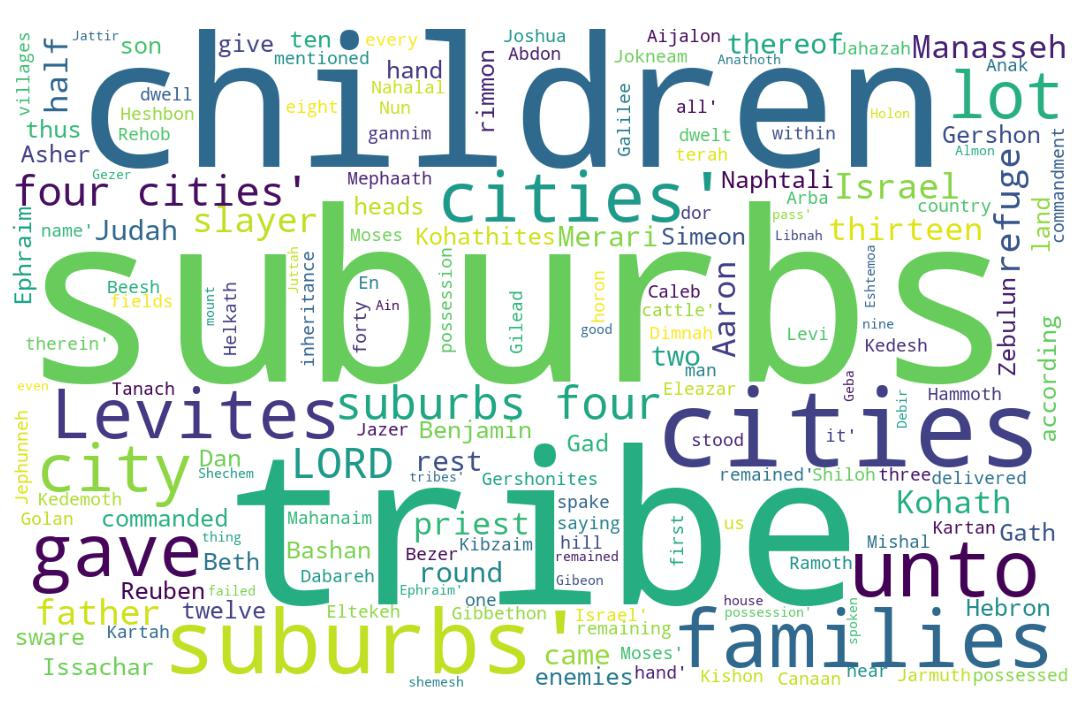
\includegraphics[width=\linewidth]{06OT-Joshua/Joshua21-WordCloud.jpg}
  \caption{Joshua 21 Word Cloud}
  \label{fig:Joshua 21 Word Cloud}
\end{figure}

\marginpar{\scriptsize \centering \fcolorbox{bone}{lime}{\textbf{CITIES FOR THE LEVITES}}\\ (Joshua 21)

\begin{compactenum}[I.][8]

    \item The \textbf{Priests} \index[scripture]{Joshua!Jsh 21:01}\index[scripture]{Joshua!Jsh 21:04}\index[scripture]{Joshua!Jsh 21:13}\index[scripture]{Joshua!Jsh 21:19}  (Jsh 21:1, 4, 13, 19)
    \item A \textbf{Place} Set Aside %\index[scripture]{Joshua!Jsh 21:04} (Jsh 21:4)
    \item The \textbf{Appointing} \index[scripture]{Joshua!Jsh 21:04} (Jsh 21:4)
    \item \textbf{Pastures} \index[scripture]{Joshua!Jsh 21:09}\index[scripture]{Joshua!Jsh 21:42} (Jsh 21:9, 42)
    \item Took \textbf{Possession} \index[scripture]{Joshua!Jsh 21:12} \index[scripture]{Joshua!Jsh 21:41}  \index[scripture]{Joshua!Jsh 21:43} (Jsh 21:12, 41, 43)
    \item God's Word Come to Pass  \index[scripture]{Joshua!Jsh 21:45}  (Jsh 21:45)

\end{compactenum}}





\footnote{\textcolor[rgb]{0.00,0.25,0.00}{\hyperlink{TOC}{Return to end of Table of Contents.}}}\footnote{\href{https://audiobible.com/bible/joshua_21.html}{\textcolor[cmyk]{0.99998,1,0,0}{Joshua 21 Audio}}}\textcolor[cmyk]{0.99998,1,0,0}{Then came near the heads of the fathers of the Levites unto Eleazar the priest, and unto Joshua the son of Nun, and unto the heads of the fathers of the tribes of the children of Israel;}
[2] \textcolor[cmyk]{0.99998,1,0,0}{And they spake unto them at Shiloh in the land of Canaan, saying, The LORD commanded by the hand of Moses to give us cities to dwell in, with the suburbs thereof for our cattle.}
[3] \textcolor[cmyk]{0.99998,1,0,0}{And the children of Israel gave unto the Levites out of their inheritance, at the commandment of the LORD, these cities and their suburbs.}
[4] \textcolor[cmyk]{0.99998,1,0,0}{And the lot came out for the families of the Kohathites: and the children of Aaron the priest, \emph{which} \emph{were} of the Levites, had by lot out of the tribe of Judah, and out of the tribe of Simeon, and out of the tribe of Benjamin, thirteen cities.}
[5] \textcolor[cmyk]{0.99998,1,0,0}{And the rest of the children of Kohath \emph{had} by lot out of the families of the tribe of Ephraim, and out of the tribe of Dan, and out of the half tribe of Manasseh, ten cities.}
[6] \textcolor[cmyk]{0.99998,1,0,0}{And the children of Gershon \emph{had} by lot out of the families of the tribe of Issachar, and out of the tribe of Asher, and out of the tribe of Naphtali, and out of the half tribe of Manasseh in Bashan, thirteen cities.}
[7] \textcolor[cmyk]{0.99998,1,0,0}{The children of Merari by their families \emph{had} out of the tribe of Reuben, and out of the tribe of Gad, and out of the tribe of Zebulun, twelve cities.}
[8] \textcolor[cmyk]{0.99998,1,0,0}{And the children of Israel gave by lot unto the Levites these cities with their suburbs, as the LORD commanded by the hand of Moses.}\\
\\
\P \textcolor[cmyk]{0.99998,1,0,0}{And they gave out of the tribe of the children of Judah, and out of the tribe of the children of Simeon, these cities which are \emph{here} mentioned by name,}
[10] \textcolor[cmyk]{0.99998,1,0,0}{Which the children of Aaron, \emph{being} of the families of the Kohathites, \emph{who} \emph{were} of the children of Levi, had: for their's was the first lot.}
[11] \textcolor[cmyk]{0.99998,1,0,0}{And they gave them the city of Arba the father of Anak, which \emph{city} \emph{is} Hebron, in the hill \emph{country} of Judah, with the suburbs thereof round about it.}
[12] \textcolor[cmyk]{0.99998,1,0,0}{But the fields of the city, and the villages thereof, gave they to Caleb the son of Jephunneh for his possession.}\\
\\
\P \textcolor[cmyk]{0.99998,1,0,0}{Thus they gave to the children of Aaron the priest Hebron with her suburbs, \emph{to} \emph{be} a city of refuge for the slayer; and Libnah with her suburbs,}
[14] \textcolor[cmyk]{0.99998,1,0,0}{And Jattir with her suburbs, and Eshtemoa with her suburbs,}
[15] \textcolor[cmyk]{0.99998,1,0,0}{And Holon with her suburbs, and Debir with her suburbs,}
[16] \textcolor[cmyk]{0.99998,1,0,0}{And Ain with her suburbs, and Juttah with her suburbs, \emph{and} Beth-shemesh with her suburbs; nine cities out of those two tribes.}
[17] \textcolor[cmyk]{0.99998,1,0,0}{And out of the tribe of Benjamin, Gibeon with her suburbs, Geba with her suburbs,}
[18] \textcolor[cmyk]{0.99998,1,0,0}{Anathoth with her suburbs, and Almon with her suburbs; four cities.}
[19] \textcolor[cmyk]{0.99998,1,0,0}{All the cities of the children of Aaron, the priests, \emph{were} thirteen cities with their suburbs.}\\
\\
\P \textcolor[cmyk]{0.99998,1,0,0}{And the families of the children of Kohath, the Levites which remained of the children of Kohath, even they had the cities of their lot out of the tribe of Ephraim.}
[21] \textcolor[cmyk]{0.99998,1,0,0}{For they gave them Shechem with her suburbs in mount Ephraim, \emph{to} \emph{be} a city of refuge for the slayer; and Gezer with her suburbs,}
[22] \textcolor[cmyk]{0.99998,1,0,0}{And Kibzaim with her suburbs, and Beth-horon with her suburbs; four cities.}
[23] \textcolor[cmyk]{0.99998,1,0,0}{And out of the tribe of Dan, Eltekeh with her suburbs, Gibbethon with her suburbs,}
[24] \textcolor[cmyk]{0.99998,1,0,0}{Aijalon with her suburbs, Gath-rimmon with her suburbs; four cities.}
[25] \textcolor[cmyk]{0.99998,1,0,0}{And out of the half tribe of Manasseh, Tanach with her suburbs, and Gath-rimmon with her suburbs; two cities.}
[26] \textcolor[cmyk]{0.99998,1,0,0}{All the cities \emph{were} ten with their suburbs for the families of the children of Kohath that remained.}\\
\\
\P \textcolor[cmyk]{0.99998,1,0,0}{And unto the children of Gershon, of the families of the Levites, out of the \emph{other} half tribe of Manasseh \emph{they} \emph{gave} Golan in Bashan with her suburbs, \emph{to} \emph{be} a city of refuge for the slayer; and Beesh-terah with her suburbs; two cities.}
[28] \textcolor[cmyk]{0.99998,1,0,0}{And out of the tribe of Issachar, Kishon with her suburbs, Dabareh with her suburbs,}
[29] \textcolor[cmyk]{0.99998,1,0,0}{Jarmuth with her suburbs, En-gannim with her suburbs; four cities.}
[30] \textcolor[cmyk]{0.99998,1,0,0}{And out of the tribe of Asher, Mishal with her suburbs, Abdon with her suburbs,}
[31] \textcolor[cmyk]{0.99998,1,0,0}{Helkath with her suburbs, and Rehob with her suburbs; four cities.}
[32] \textcolor[cmyk]{0.99998,1,0,0}{And out of the tribe of Naphtali, Kedesh in Galilee with her suburbs, \emph{to} \emph{be} a city of refuge for the slayer; and Hammoth-dor with her suburbs, and Kartan with her suburbs; three cities.}
[33] \textcolor[cmyk]{0.99998,1,0,0}{All the cities of the Gershonites according to their families \emph{were} thirteen cities with their suburbs.}\\
\\
\P \textcolor[cmyk]{0.99998,1,0,0}{And unto the families of the children of Merari, the rest of the Levites, out of the tribe of Zebulun, Jokneam with her suburbs, and Kartah with her suburbs,}
[35] \textcolor[cmyk]{0.99998,1,0,0}{Dimnah with her suburbs, Nahalal with her suburbs; four cities.}
[36] \textcolor[cmyk]{0.99998,1,0,0}{And out of the tribe of Reuben, Bezer with her suburbs, and Jahazah with her suburbs,}
[37] \textcolor[cmyk]{0.99998,1,0,0}{Kedemoth with her suburbs, and Mephaath with her suburbs; four cities.}
[38] \textcolor[cmyk]{0.99998,1,0,0}{And out of the tribe of Gad, Ramoth in Gilead with her suburbs, \emph{to} \emph{be} a city of refuge for the slayer; and Mahanaim with her suburbs,}
[39] \textcolor[cmyk]{0.99998,1,0,0}{Heshbon with her suburbs, Jazer with her suburbs; four cities in all.}\\
\\
\P \textcolor[cmyk]{0.99998,1,0,0}{And the LORD gave unto Israel all the land which he sware to give unto their fathers; and they possessed it, and dwelt therein.}
[44] \textcolor[cmyk]{0.99998,1,0,0}{And the LORD gave them rest round about, according to all that he sware unto their fathers: and there stood not a man of all their enemies before them; the LORD delivered all their enemies into their hand.}
[45] \textcolor[cmyk]{0.99998,1,0,0}{There failed not ought of any good thing which the LORD had spoken unto the house of Israel; all came to pass.}
\index[NWIV]{37!Joshua!Jos 21:1}\index[AWIP]{Then!Joshua!Jos 21:1}\index[AWIP]{came!Joshua!Jos 21:1}\index[AWIP]{near!Joshua!Jos 21:1}\index[AWIP]{the!Joshua!Jos 21:1}\index[AWIP]{the!Joshua!Jos 21:1 (2)}\index[AWIP]{the!Joshua!Jos 21:1 (3)}\index[AWIP]{the!Joshua!Jos 21:1 (4)}\index[AWIP]{the!Joshua!Jos 21:1 (5)}\index[AWIP]{the!Joshua!Jos 21:1 (6)}\index[AWIP]{the!Joshua!Jos 21:1 (7)}\index[AWIP]{the!Joshua!Jos 21:1 (8)}\index[AWIP]{the!Joshua!Jos 21:1 (9)}\index[AWIP]{heads!Joshua!Jos 21:1}\index[AWIP]{heads!Joshua!Jos 21:1 (2)}\index[AWIP]{of!Joshua!Jos 21:1}\index[AWIP]{of!Joshua!Jos 21:1 (2)}\index[AWIP]{of!Joshua!Jos 21:1 (3)}\index[AWIP]{of!Joshua!Jos 21:1 (4)}\index[AWIP]{of!Joshua!Jos 21:1 (5)}\index[AWIP]{of!Joshua!Jos 21:1 (6)}\index[AWIP]{of!Joshua!Jos 21:1 (7)}\index[AWIP]{fathers!Joshua!Jos 21:1}\index[AWIP]{fathers!Joshua!Jos 21:1 (2)}\index[AWIP]{Levites!Joshua!Jos 21:1}\index[AWIP]{unto!Joshua!Jos 21:1}\index[AWIP]{unto!Joshua!Jos 21:1 (2)}\index[AWIP]{unto!Joshua!Jos 21:1 (3)}\index[AWIP]{Eleazar!Joshua!Jos 21:1}\index[AWIP]{priest!Joshua!Jos 21:1}\index[AWIP]{and!Joshua!Jos 21:1}\index[AWIP]{and!Joshua!Jos 21:1 (2)}\index[AWIP]{Joshua!Joshua!Jos 21:1}\index[AWIP]{son!Joshua!Jos 21:1}\index[AWIP]{Nun!Joshua!Jos 21:1}\index[AWIP]{tribes!Joshua!Jos 21:1}\index[AWIP]{children!Joshua!Jos 21:1}\index[AWIP]{Israel!Joshua!Jos 21:1}

\index[NWIV]{35!Joshua!Jos 21:2}\index[AWIP]{And!Joshua!Jos 21:2}\index[AWIP]{they!Joshua!Jos 21:2}\index[AWIP]{spake!Joshua!Jos 21:2}\index[AWIP]{unto!Joshua!Jos 21:2}\index[AWIP]{them!Joshua!Jos 21:2}\index[AWIP]{at!Joshua!Jos 21:2}\index[AWIP]{Shiloh!Joshua!Jos 21:2}\index[AWIP]{in!Joshua!Jos 21:2}\index[AWIP]{in!Joshua!Jos 21:2 (2)}\index[AWIP]{the!Joshua!Jos 21:2}\index[AWIP]{the!Joshua!Jos 21:2 (2)}\index[AWIP]{the!Joshua!Jos 21:2 (3)}\index[AWIP]{land!Joshua!Jos 21:2}\index[AWIP]{of!Joshua!Jos 21:2}\index[AWIP]{of!Joshua!Jos 21:2 (2)}\index[AWIP]{Canaan!Joshua!Jos 21:2}\index[AWIP]{saying!Joshua!Jos 21:2}\index[AWIP]{The!Joshua!Jos 21:2}\index[AWIP]{LORD!Joshua!Jos 21:2}\index[AWIP]{commanded!Joshua!Jos 21:2}\index[AWIP]{by!Joshua!Jos 21:2}\index[AWIP]{hand!Joshua!Jos 21:2}\index[AWIP]{Moses!Joshua!Jos 21:2}\index[AWIP]{to!Joshua!Jos 21:2}\index[AWIP]{to!Joshua!Jos 21:2 (2)}\index[AWIP]{give!Joshua!Jos 21:2}\index[AWIP]{us!Joshua!Jos 21:2}\index[AWIP]{cities!Joshua!Jos 21:2}\index[AWIP]{dwell!Joshua!Jos 21:2}\index[AWIP]{with!Joshua!Jos 21:2}\index[AWIP]{suburbs!Joshua!Jos 21:2}\index[AWIP]{thereof!Joshua!Jos 21:2}\index[AWIP]{for!Joshua!Jos 21:2}\index[AWIP]{our!Joshua!Jos 21:2}\index[AWIP]{cattle!Joshua!Jos 21:2}

\index[NWIV]{24!Joshua!Jos 21:3}\index[AWIP]{And!Joshua!Jos 21:3}\index[AWIP]{the!Joshua!Jos 21:3}\index[AWIP]{the!Joshua!Jos 21:3 (2)}\index[AWIP]{the!Joshua!Jos 21:3 (3)}\index[AWIP]{the!Joshua!Jos 21:3 (4)}\index[AWIP]{children!Joshua!Jos 21:3}\index[AWIP]{of!Joshua!Jos 21:3}\index[AWIP]{of!Joshua!Jos 21:3 (2)}\index[AWIP]{of!Joshua!Jos 21:3 (3)}\index[AWIP]{Israel!Joshua!Jos 21:3}\index[AWIP]{gave!Joshua!Jos 21:3}\index[AWIP]{unto!Joshua!Jos 21:3}\index[AWIP]{Levites!Joshua!Jos 21:3}\index[AWIP]{out!Joshua!Jos 21:3}\index[AWIP]{their!Joshua!Jos 21:3}\index[AWIP]{their!Joshua!Jos 21:3 (2)}\index[AWIP]{inheritance!Joshua!Jos 21:3}\index[AWIP]{at!Joshua!Jos 21:3}\index[AWIP]{commandment!Joshua!Jos 21:3}\index[AWIP]{LORD!Joshua!Jos 21:3}\index[AWIP]{these!Joshua!Jos 21:3}\index[AWIP]{cities!Joshua!Jos 21:3}\index[AWIP]{and!Joshua!Jos 21:3}\index[AWIP]{suburbs!Joshua!Jos 21:3}

\index[NWIV]{48!Joshua!Jos 21:4}\index[AWIP]{And!Joshua!Jos 21:4}\index[AWIP]{the!Joshua!Jos 21:4}\index[AWIP]{the!Joshua!Jos 21:4 (2)}\index[AWIP]{the!Joshua!Jos 21:4 (3)}\index[AWIP]{the!Joshua!Jos 21:4 (4)}\index[AWIP]{the!Joshua!Jos 21:4 (5)}\index[AWIP]{the!Joshua!Jos 21:4 (6)}\index[AWIP]{the!Joshua!Jos 21:4 (7)}\index[AWIP]{the!Joshua!Jos 21:4 (8)}\index[AWIP]{the!Joshua!Jos 21:4 (9)}\index[AWIP]{lot!Joshua!Jos 21:4}\index[AWIP]{lot!Joshua!Jos 21:4 (2)}\index[AWIP]{came!Joshua!Jos 21:4}\index[AWIP]{out!Joshua!Jos 21:4}\index[AWIP]{out!Joshua!Jos 21:4 (2)}\index[AWIP]{out!Joshua!Jos 21:4 (3)}\index[AWIP]{out!Joshua!Jos 21:4 (4)}\index[AWIP]{for!Joshua!Jos 21:4}\index[AWIP]{families!Joshua!Jos 21:4}\index[AWIP]{of!Joshua!Jos 21:4}\index[AWIP]{of!Joshua!Jos 21:4 (2)}\index[AWIP]{of!Joshua!Jos 21:4 (3)}\index[AWIP]{of!Joshua!Jos 21:4 (4)}\index[AWIP]{of!Joshua!Jos 21:4 (5)}\index[AWIP]{of!Joshua!Jos 21:4 (6)}\index[AWIP]{of!Joshua!Jos 21:4 (7)}\index[AWIP]{of!Joshua!Jos 21:4 (8)}\index[AWIP]{of!Joshua!Jos 21:4 (9)}\index[AWIP]{Kohathites!Joshua!Jos 21:4}\index[AWIP]{and!Joshua!Jos 21:4}\index[AWIP]{and!Joshua!Jos 21:4 (2)}\index[AWIP]{and!Joshua!Jos 21:4 (3)}\index[AWIP]{children!Joshua!Jos 21:4}\index[AWIP]{Aaron!Joshua!Jos 21:4}\index[AWIP]{priest!Joshua!Jos 21:4}\index[AWIP]{\emph{which}!Joshua!Jos 21:4}\index[AWIP]{\emph{were}!Joshua!Jos 21:4}\index[AWIP]{Levites!Joshua!Jos 21:4}\index[AWIP]{had!Joshua!Jos 21:4}\index[AWIP]{by!Joshua!Jos 21:4}\index[AWIP]{tribe!Joshua!Jos 21:4}\index[AWIP]{tribe!Joshua!Jos 21:4 (2)}\index[AWIP]{tribe!Joshua!Jos 21:4 (3)}\index[AWIP]{Judah!Joshua!Jos 21:4}\index[AWIP]{Simeon!Joshua!Jos 21:4}\index[AWIP]{Benjamin!Joshua!Jos 21:4}\index[AWIP]{thirteen!Joshua!Jos 21:4}\index[AWIP]{cities!Joshua!Jos 21:4}\index[AWIP]{\emph{which}!Joshua!Jos 21:4}\index[AWIP]{\emph{were}!Joshua!Jos 21:4}

\index[NWIV]{37!Joshua!Jos 21:5}\index[AWIP]{And!Joshua!Jos 21:5}\index[AWIP]{the!Joshua!Jos 21:5}\index[AWIP]{the!Joshua!Jos 21:5 (2)}\index[AWIP]{the!Joshua!Jos 21:5 (3)}\index[AWIP]{the!Joshua!Jos 21:5 (4)}\index[AWIP]{the!Joshua!Jos 21:5 (5)}\index[AWIP]{the!Joshua!Jos 21:5 (6)}\index[AWIP]{rest!Joshua!Jos 21:5}\index[AWIP]{of!Joshua!Jos 21:5}\index[AWIP]{of!Joshua!Jos 21:5 (2)}\index[AWIP]{of!Joshua!Jos 21:5 (3)}\index[AWIP]{of!Joshua!Jos 21:5 (4)}\index[AWIP]{of!Joshua!Jos 21:5 (5)}\index[AWIP]{of!Joshua!Jos 21:5 (6)}\index[AWIP]{of!Joshua!Jos 21:5 (7)}\index[AWIP]{of!Joshua!Jos 21:5 (8)}\index[AWIP]{of!Joshua!Jos 21:5 (9)}\index[AWIP]{children!Joshua!Jos 21:5}\index[AWIP]{Kohath!Joshua!Jos 21:5}\index[AWIP]{\emph{had}!Joshua!Jos 21:5}\index[AWIP]{by!Joshua!Jos 21:5}\index[AWIP]{lot!Joshua!Jos 21:5}\index[AWIP]{out!Joshua!Jos 21:5}\index[AWIP]{out!Joshua!Jos 21:5 (2)}\index[AWIP]{out!Joshua!Jos 21:5 (3)}\index[AWIP]{families!Joshua!Jos 21:5}\index[AWIP]{tribe!Joshua!Jos 21:5}\index[AWIP]{tribe!Joshua!Jos 21:5 (2)}\index[AWIP]{tribe!Joshua!Jos 21:5 (3)}\index[AWIP]{Ephraim!Joshua!Jos 21:5}\index[AWIP]{and!Joshua!Jos 21:5}\index[AWIP]{and!Joshua!Jos 21:5 (2)}\index[AWIP]{Dan!Joshua!Jos 21:5}\index[AWIP]{half!Joshua!Jos 21:5}\index[AWIP]{Manasseh!Joshua!Jos 21:5}\index[AWIP]{ten!Joshua!Jos 21:5}\index[AWIP]{cities!Joshua!Jos 21:5}\index[AWIP]{\emph{had}!Joshua!Jos 21:5}

\index[NWIV]{43!Joshua!Jos 21:6}\index[AWIP]{And!Joshua!Jos 21:6}\index[AWIP]{the!Joshua!Jos 21:6}\index[AWIP]{the!Joshua!Jos 21:6 (2)}\index[AWIP]{the!Joshua!Jos 21:6 (3)}\index[AWIP]{the!Joshua!Jos 21:6 (4)}\index[AWIP]{the!Joshua!Jos 21:6 (5)}\index[AWIP]{the!Joshua!Jos 21:6 (6)}\index[AWIP]{children!Joshua!Jos 21:6}\index[AWIP]{of!Joshua!Jos 21:6}\index[AWIP]{of!Joshua!Jos 21:6 (2)}\index[AWIP]{of!Joshua!Jos 21:6 (3)}\index[AWIP]{of!Joshua!Jos 21:6 (4)}\index[AWIP]{of!Joshua!Jos 21:6 (5)}\index[AWIP]{of!Joshua!Jos 21:6 (6)}\index[AWIP]{of!Joshua!Jos 21:6 (7)}\index[AWIP]{of!Joshua!Jos 21:6 (8)}\index[AWIP]{of!Joshua!Jos 21:6 (9)}\index[AWIP]{of!Joshua!Jos 21:6 (10)}\index[AWIP]{Gershon!Joshua!Jos 21:6}\index[AWIP]{\emph{had}!Joshua!Jos 21:6}\index[AWIP]{by!Joshua!Jos 21:6}\index[AWIP]{lot!Joshua!Jos 21:6}\index[AWIP]{out!Joshua!Jos 21:6}\index[AWIP]{out!Joshua!Jos 21:6 (2)}\index[AWIP]{out!Joshua!Jos 21:6 (3)}\index[AWIP]{out!Joshua!Jos 21:6 (4)}\index[AWIP]{families!Joshua!Jos 21:6}\index[AWIP]{tribe!Joshua!Jos 21:6}\index[AWIP]{tribe!Joshua!Jos 21:6 (2)}\index[AWIP]{tribe!Joshua!Jos 21:6 (3)}\index[AWIP]{tribe!Joshua!Jos 21:6 (4)}\index[AWIP]{Issachar!Joshua!Jos 21:6}\index[AWIP]{and!Joshua!Jos 21:6}\index[AWIP]{and!Joshua!Jos 21:6 (2)}\index[AWIP]{and!Joshua!Jos 21:6 (3)}\index[AWIP]{Asher!Joshua!Jos 21:6}\index[AWIP]{Naphtali!Joshua!Jos 21:6}\index[AWIP]{half!Joshua!Jos 21:6}\index[AWIP]{Manasseh!Joshua!Jos 21:6}\index[AWIP]{in!Joshua!Jos 21:6}\index[AWIP]{Bashan!Joshua!Jos 21:6}\index[AWIP]{thirteen!Joshua!Jos 21:6}\index[AWIP]{cities!Joshua!Jos 21:6}\index[AWIP]{\emph{had}!Joshua!Jos 21:6}

\index[NWIV]{30!Joshua!Jos 21:7}\index[AWIP]{The!Joshua!Jos 21:7}\index[AWIP]{children!Joshua!Jos 21:7}\index[AWIP]{of!Joshua!Jos 21:7}\index[AWIP]{of!Joshua!Jos 21:7 (2)}\index[AWIP]{of!Joshua!Jos 21:7 (3)}\index[AWIP]{of!Joshua!Jos 21:7 (4)}\index[AWIP]{of!Joshua!Jos 21:7 (5)}\index[AWIP]{of!Joshua!Jos 21:7 (6)}\index[AWIP]{of!Joshua!Jos 21:7 (7)}\index[AWIP]{Merari!Joshua!Jos 21:7}\index[AWIP]{by!Joshua!Jos 21:7}\index[AWIP]{their!Joshua!Jos 21:7}\index[AWIP]{families!Joshua!Jos 21:7}\index[AWIP]{\emph{had}!Joshua!Jos 21:7}\index[AWIP]{out!Joshua!Jos 21:7}\index[AWIP]{out!Joshua!Jos 21:7 (2)}\index[AWIP]{out!Joshua!Jos 21:7 (3)}\index[AWIP]{the!Joshua!Jos 21:7}\index[AWIP]{the!Joshua!Jos 21:7 (2)}\index[AWIP]{the!Joshua!Jos 21:7 (3)}\index[AWIP]{tribe!Joshua!Jos 21:7}\index[AWIP]{tribe!Joshua!Jos 21:7 (2)}\index[AWIP]{tribe!Joshua!Jos 21:7 (3)}\index[AWIP]{Reuben!Joshua!Jos 21:7}\index[AWIP]{and!Joshua!Jos 21:7}\index[AWIP]{and!Joshua!Jos 21:7 (2)}\index[AWIP]{Gad!Joshua!Jos 21:7}\index[AWIP]{Zebulun!Joshua!Jos 21:7}\index[AWIP]{twelve!Joshua!Jos 21:7}\index[AWIP]{cities!Joshua!Jos 21:7}\index[AWIP]{\emph{had}!Joshua!Jos 21:7}

\index[NWIV]{25!Joshua!Jos 21:8}\index[AWIP]{And!Joshua!Jos 21:8}\index[AWIP]{the!Joshua!Jos 21:8}\index[AWIP]{the!Joshua!Jos 21:8 (2)}\index[AWIP]{the!Joshua!Jos 21:8 (3)}\index[AWIP]{the!Joshua!Jos 21:8 (4)}\index[AWIP]{children!Joshua!Jos 21:8}\index[AWIP]{of!Joshua!Jos 21:8}\index[AWIP]{of!Joshua!Jos 21:8 (2)}\index[AWIP]{Israel!Joshua!Jos 21:8}\index[AWIP]{gave!Joshua!Jos 21:8}\index[AWIP]{by!Joshua!Jos 21:8}\index[AWIP]{by!Joshua!Jos 21:8 (2)}\index[AWIP]{lot!Joshua!Jos 21:8}\index[AWIP]{unto!Joshua!Jos 21:8}\index[AWIP]{Levites!Joshua!Jos 21:8}\index[AWIP]{these!Joshua!Jos 21:8}\index[AWIP]{cities!Joshua!Jos 21:8}\index[AWIP]{with!Joshua!Jos 21:8}\index[AWIP]{their!Joshua!Jos 21:8}\index[AWIP]{suburbs!Joshua!Jos 21:8}\index[AWIP]{as!Joshua!Jos 21:8}\index[AWIP]{LORD!Joshua!Jos 21:8}\index[AWIP]{commanded!Joshua!Jos 21:8}\index[AWIP]{hand!Joshua!Jos 21:8}\index[AWIP]{Moses!Joshua!Jos 21:8}

\index[NWIV]{30!Joshua!Jos 21:9}\index[AWIP]{And!Joshua!Jos 21:9}\index[AWIP]{they!Joshua!Jos 21:9}\index[AWIP]{gave!Joshua!Jos 21:9}\index[AWIP]{out!Joshua!Jos 21:9}\index[AWIP]{out!Joshua!Jos 21:9 (2)}\index[AWIP]{of!Joshua!Jos 21:9}\index[AWIP]{of!Joshua!Jos 21:9 (2)}\index[AWIP]{of!Joshua!Jos 21:9 (3)}\index[AWIP]{of!Joshua!Jos 21:9 (4)}\index[AWIP]{of!Joshua!Jos 21:9 (5)}\index[AWIP]{of!Joshua!Jos 21:9 (6)}\index[AWIP]{the!Joshua!Jos 21:9}\index[AWIP]{the!Joshua!Jos 21:9 (2)}\index[AWIP]{the!Joshua!Jos 21:9 (3)}\index[AWIP]{the!Joshua!Jos 21:9 (4)}\index[AWIP]{tribe!Joshua!Jos 21:9}\index[AWIP]{tribe!Joshua!Jos 21:9 (2)}\index[AWIP]{children!Joshua!Jos 21:9}\index[AWIP]{children!Joshua!Jos 21:9 (2)}\index[AWIP]{Judah!Joshua!Jos 21:9}\index[AWIP]{and!Joshua!Jos 21:9}\index[AWIP]{Simeon!Joshua!Jos 21:9}\index[AWIP]{these!Joshua!Jos 21:9}\index[AWIP]{cities!Joshua!Jos 21:9}\index[AWIP]{which!Joshua!Jos 21:9}\index[AWIP]{are!Joshua!Jos 21:9}\index[AWIP]{\emph{here}!Joshua!Jos 21:9}\index[AWIP]{mentioned!Joshua!Jos 21:9}\index[AWIP]{by!Joshua!Jos 21:9}\index[AWIP]{name!Joshua!Jos 21:9}\index[AWIP]{\emph{here}!Joshua!Jos 21:9}

\index[NWIV]{26!Joshua!Jos 21:10}\index[AWIP]{Which!Joshua!Jos 21:10}\index[AWIP]{the!Joshua!Jos 21:10}\index[AWIP]{the!Joshua!Jos 21:10 (2)}\index[AWIP]{the!Joshua!Jos 21:10 (3)}\index[AWIP]{the!Joshua!Jos 21:10 (4)}\index[AWIP]{the!Joshua!Jos 21:10 (5)}\index[AWIP]{children!Joshua!Jos 21:10}\index[AWIP]{children!Joshua!Jos 21:10 (2)}\index[AWIP]{of!Joshua!Jos 21:10}\index[AWIP]{of!Joshua!Jos 21:10 (2)}\index[AWIP]{of!Joshua!Jos 21:10 (3)}\index[AWIP]{of!Joshua!Jos 21:10 (4)}\index[AWIP]{of!Joshua!Jos 21:10 (5)}\index[AWIP]{Aaron!Joshua!Jos 21:10}\index[AWIP]{\emph{being}!Joshua!Jos 21:10}\index[AWIP]{families!Joshua!Jos 21:10}\index[AWIP]{Kohathites!Joshua!Jos 21:10}\index[AWIP]{\emph{who}!Joshua!Jos 21:10}\index[AWIP]{\emph{were}!Joshua!Jos 21:10}\index[AWIP]{Levi!Joshua!Jos 21:10}\index[AWIP]{had!Joshua!Jos 21:10}\index[AWIP]{for!Joshua!Jos 21:10}\index[AWIP]{their's!Joshua!Jos 21:10}\index[AWIP]{was!Joshua!Jos 21:10}\index[AWIP]{first!Joshua!Jos 21:10}\index[AWIP]{lot!Joshua!Jos 21:10}\index[AWIP]{\emph{being}!Joshua!Jos 21:10}\index[AWIP]{\emph{who}!Joshua!Jos 21:10}\index[AWIP]{\emph{were}!Joshua!Jos 21:10}

\index[NWIV]{29!Joshua!Jos 21:11}\index[AWIP]{And!Joshua!Jos 21:11}\index[AWIP]{they!Joshua!Jos 21:11}\index[AWIP]{gave!Joshua!Jos 21:11}\index[AWIP]{them!Joshua!Jos 21:11}\index[AWIP]{the!Joshua!Jos 21:11}\index[AWIP]{the!Joshua!Jos 21:11 (2)}\index[AWIP]{the!Joshua!Jos 21:11 (3)}\index[AWIP]{the!Joshua!Jos 21:11 (4)}\index[AWIP]{city!Joshua!Jos 21:11}\index[AWIP]{of!Joshua!Jos 21:11}\index[AWIP]{of!Joshua!Jos 21:11 (2)}\index[AWIP]{of!Joshua!Jos 21:11 (3)}\index[AWIP]{Arba!Joshua!Jos 21:11}\index[AWIP]{father!Joshua!Jos 21:11}\index[AWIP]{Anak!Joshua!Jos 21:11}\index[AWIP]{which!Joshua!Jos 21:11}\index[AWIP]{\emph{city}!Joshua!Jos 21:11}\index[AWIP]{\emph{is}!Joshua!Jos 21:11}\index[AWIP]{Hebron!Joshua!Jos 21:11}\index[AWIP]{in!Joshua!Jos 21:11}\index[AWIP]{hill!Joshua!Jos 21:11}\index[AWIP]{\emph{country}!Joshua!Jos 21:11}\index[AWIP]{Judah!Joshua!Jos 21:11}\index[AWIP]{with!Joshua!Jos 21:11}\index[AWIP]{suburbs!Joshua!Jos 21:11}\index[AWIP]{thereof!Joshua!Jos 21:11}\index[AWIP]{round!Joshua!Jos 21:11}\index[AWIP]{about!Joshua!Jos 21:11}\index[AWIP]{it!Joshua!Jos 21:11}\index[AWIP]{\emph{city}!Joshua!Jos 21:11}\index[AWIP]{\emph{is}!Joshua!Jos 21:11}\index[AWIP]{\emph{country}!Joshua!Jos 21:11}

\index[NWIV]{21!Joshua!Jos 21:12}\index[AWIP]{But!Joshua!Jos 21:12}\index[AWIP]{the!Joshua!Jos 21:12}\index[AWIP]{the!Joshua!Jos 21:12 (2)}\index[AWIP]{the!Joshua!Jos 21:12 (3)}\index[AWIP]{the!Joshua!Jos 21:12 (4)}\index[AWIP]{fields!Joshua!Jos 21:12}\index[AWIP]{of!Joshua!Jos 21:12}\index[AWIP]{of!Joshua!Jos 21:12 (2)}\index[AWIP]{city!Joshua!Jos 21:12}\index[AWIP]{and!Joshua!Jos 21:12}\index[AWIP]{villages!Joshua!Jos 21:12}\index[AWIP]{thereof!Joshua!Jos 21:12}\index[AWIP]{gave!Joshua!Jos 21:12}\index[AWIP]{they!Joshua!Jos 21:12}\index[AWIP]{to!Joshua!Jos 21:12}\index[AWIP]{Caleb!Joshua!Jos 21:12}\index[AWIP]{son!Joshua!Jos 21:12}\index[AWIP]{Jephunneh!Joshua!Jos 21:12}\index[AWIP]{for!Joshua!Jos 21:12}\index[AWIP]{his!Joshua!Jos 21:12}\index[AWIP]{possession!Joshua!Jos 21:12}

\index[NWIV]{28!Joshua!Jos 21:13}\index[AWIP]{Thus!Joshua!Jos 21:13}\index[AWIP]{they!Joshua!Jos 21:13}\index[AWIP]{gave!Joshua!Jos 21:13}\index[AWIP]{to!Joshua!Jos 21:13}\index[AWIP]{the!Joshua!Jos 21:13}\index[AWIP]{the!Joshua!Jos 21:13 (2)}\index[AWIP]{the!Joshua!Jos 21:13 (3)}\index[AWIP]{children!Joshua!Jos 21:13}\index[AWIP]{of!Joshua!Jos 21:13}\index[AWIP]{of!Joshua!Jos 21:13 (2)}\index[AWIP]{Aaron!Joshua!Jos 21:13}\index[AWIP]{priest!Joshua!Jos 21:13}\index[AWIP]{Hebron!Joshua!Jos 21:13}\index[AWIP]{with!Joshua!Jos 21:13}\index[AWIP]{with!Joshua!Jos 21:13 (2)}\index[AWIP]{her!Joshua!Jos 21:13}\index[AWIP]{her!Joshua!Jos 21:13 (2)}\index[AWIP]{suburbs!Joshua!Jos 21:13}\index[AWIP]{suburbs!Joshua!Jos 21:13 (2)}\index[AWIP]{\emph{to}!Joshua!Jos 21:13}\index[AWIP]{\emph{be}!Joshua!Jos 21:13}\index[AWIP]{a!Joshua!Jos 21:13}\index[AWIP]{city!Joshua!Jos 21:13}\index[AWIP]{refuge!Joshua!Jos 21:13}\index[AWIP]{for!Joshua!Jos 21:13}\index[AWIP]{slayer!Joshua!Jos 21:13}\index[AWIP]{and!Joshua!Jos 21:13}\index[AWIP]{Libnah!Joshua!Jos 21:13}\index[AWIP]{\emph{to}!Joshua!Jos 21:13}\index[AWIP]{\emph{be}!Joshua!Jos 21:13}

\index[NWIV]{10!Joshua!Jos 21:14}\index[AWIP]{And!Joshua!Jos 21:14}\index[AWIP]{Jattir!Joshua!Jos 21:14}\index[AWIP]{with!Joshua!Jos 21:14}\index[AWIP]{with!Joshua!Jos 21:14 (2)}\index[AWIP]{her!Joshua!Jos 21:14}\index[AWIP]{her!Joshua!Jos 21:14 (2)}\index[AWIP]{suburbs!Joshua!Jos 21:14}\index[AWIP]{suburbs!Joshua!Jos 21:14 (2)}\index[AWIP]{and!Joshua!Jos 21:14}\index[AWIP]{Eshtemoa!Joshua!Jos 21:14}

\index[NWIV]{10!Joshua!Jos 21:15}\index[AWIP]{And!Joshua!Jos 21:15}\index[AWIP]{Holon!Joshua!Jos 21:15}\index[AWIP]{with!Joshua!Jos 21:15}\index[AWIP]{with!Joshua!Jos 21:15 (2)}\index[AWIP]{her!Joshua!Jos 21:15}\index[AWIP]{her!Joshua!Jos 21:15 (2)}\index[AWIP]{suburbs!Joshua!Jos 21:15}\index[AWIP]{suburbs!Joshua!Jos 21:15 (2)}\index[AWIP]{and!Joshua!Jos 21:15}\index[AWIP]{Debir!Joshua!Jos 21:15}

\index[NWIV]{22!Joshua!Jos 21:16}\index[AWIP]{And!Joshua!Jos 21:16}\index[AWIP]{Ain!Joshua!Jos 21:16}\index[AWIP]{with!Joshua!Jos 21:16}\index[AWIP]{with!Joshua!Jos 21:16 (2)}\index[AWIP]{with!Joshua!Jos 21:16 (3)}\index[AWIP]{her!Joshua!Jos 21:16}\index[AWIP]{her!Joshua!Jos 21:16 (2)}\index[AWIP]{her!Joshua!Jos 21:16 (3)}\index[AWIP]{suburbs!Joshua!Jos 21:16}\index[AWIP]{suburbs!Joshua!Jos 21:16 (2)}\index[AWIP]{suburbs!Joshua!Jos 21:16 (3)}\index[AWIP]{and!Joshua!Jos 21:16}\index[AWIP]{Juttah!Joshua!Jos 21:16}\index[AWIP]{\emph{and}!Joshua!Jos 21:16}\index[AWIP]{Beth-shemesh!Joshua!Jos 21:16}\index[AWIP]{nine!Joshua!Jos 21:16}\index[AWIP]{cities!Joshua!Jos 21:16}\index[AWIP]{out!Joshua!Jos 21:16}\index[AWIP]{of!Joshua!Jos 21:16}\index[AWIP]{those!Joshua!Jos 21:16}\index[AWIP]{two!Joshua!Jos 21:16}\index[AWIP]{tribes!Joshua!Jos 21:16}\index[AWIP]{\emph{and}!Joshua!Jos 21:16}

\index[NWIV]{15!Joshua!Jos 21:17}\index[AWIP]{And!Joshua!Jos 21:17}\index[AWIP]{out!Joshua!Jos 21:17}\index[AWIP]{of!Joshua!Jos 21:17}\index[AWIP]{of!Joshua!Jos 21:17 (2)}\index[AWIP]{the!Joshua!Jos 21:17}\index[AWIP]{tribe!Joshua!Jos 21:17}\index[AWIP]{Benjamin!Joshua!Jos 21:17}\index[AWIP]{Gibeon!Joshua!Jos 21:17}\index[AWIP]{with!Joshua!Jos 21:17}\index[AWIP]{with!Joshua!Jos 21:17 (2)}\index[AWIP]{her!Joshua!Jos 21:17}\index[AWIP]{her!Joshua!Jos 21:17 (2)}\index[AWIP]{suburbs!Joshua!Jos 21:17}\index[AWIP]{suburbs!Joshua!Jos 21:17 (2)}\index[AWIP]{Geba!Joshua!Jos 21:17}

\index[NWIV]{11!Joshua!Jos 21:18}\index[AWIP]{Anathoth!Joshua!Jos 21:18}\index[AWIP]{with!Joshua!Jos 21:18}\index[AWIP]{with!Joshua!Jos 21:18 (2)}\index[AWIP]{her!Joshua!Jos 21:18}\index[AWIP]{her!Joshua!Jos 21:18 (2)}\index[AWIP]{suburbs!Joshua!Jos 21:18}\index[AWIP]{suburbs!Joshua!Jos 21:18 (2)}\index[AWIP]{and!Joshua!Jos 21:18}\index[AWIP]{Almon!Joshua!Jos 21:18}\index[AWIP]{four!Joshua!Jos 21:18}\index[AWIP]{cities!Joshua!Jos 21:18}

\index[NWIV]{16!Joshua!Jos 21:19}\index[AWIP]{All!Joshua!Jos 21:19}\index[AWIP]{the!Joshua!Jos 21:19}\index[AWIP]{the!Joshua!Jos 21:19 (2)}\index[AWIP]{the!Joshua!Jos 21:19 (3)}\index[AWIP]{cities!Joshua!Jos 21:19}\index[AWIP]{cities!Joshua!Jos 21:19 (2)}\index[AWIP]{of!Joshua!Jos 21:19}\index[AWIP]{of!Joshua!Jos 21:19 (2)}\index[AWIP]{children!Joshua!Jos 21:19}\index[AWIP]{Aaron!Joshua!Jos 21:19}\index[AWIP]{priests!Joshua!Jos 21:19}\index[AWIP]{\emph{were}!Joshua!Jos 21:19}\index[AWIP]{thirteen!Joshua!Jos 21:19}\index[AWIP]{with!Joshua!Jos 21:19}\index[AWIP]{their!Joshua!Jos 21:19}\index[AWIP]{suburbs!Joshua!Jos 21:19}\index[AWIP]{\emph{were}!Joshua!Jos 21:19}

\index[NWIV]{31!Joshua!Jos 21:20}\index[AWIP]{And!Joshua!Jos 21:20}\index[AWIP]{the!Joshua!Jos 21:20}\index[AWIP]{the!Joshua!Jos 21:20 (2)}\index[AWIP]{the!Joshua!Jos 21:20 (3)}\index[AWIP]{the!Joshua!Jos 21:20 (4)}\index[AWIP]{the!Joshua!Jos 21:20 (5)}\index[AWIP]{the!Joshua!Jos 21:20 (6)}\index[AWIP]{families!Joshua!Jos 21:20}\index[AWIP]{of!Joshua!Jos 21:20}\index[AWIP]{of!Joshua!Jos 21:20 (2)}\index[AWIP]{of!Joshua!Jos 21:20 (3)}\index[AWIP]{of!Joshua!Jos 21:20 (4)}\index[AWIP]{of!Joshua!Jos 21:20 (5)}\index[AWIP]{of!Joshua!Jos 21:20 (6)}\index[AWIP]{of!Joshua!Jos 21:20 (7)}\index[AWIP]{children!Joshua!Jos 21:20}\index[AWIP]{children!Joshua!Jos 21:20 (2)}\index[AWIP]{Kohath!Joshua!Jos 21:20}\index[AWIP]{Kohath!Joshua!Jos 21:20 (2)}\index[AWIP]{Levites!Joshua!Jos 21:20}\index[AWIP]{which!Joshua!Jos 21:20}\index[AWIP]{remained!Joshua!Jos 21:20}\index[AWIP]{even!Joshua!Jos 21:20}\index[AWIP]{they!Joshua!Jos 21:20}\index[AWIP]{had!Joshua!Jos 21:20}\index[AWIP]{cities!Joshua!Jos 21:20}\index[AWIP]{their!Joshua!Jos 21:20}\index[AWIP]{lot!Joshua!Jos 21:20}\index[AWIP]{out!Joshua!Jos 21:20}\index[AWIP]{tribe!Joshua!Jos 21:20}\index[AWIP]{Ephraim!Joshua!Jos 21:20}

\index[NWIV]{25!Joshua!Jos 21:21}\index[AWIP]{For!Joshua!Jos 21:21}\index[AWIP]{they!Joshua!Jos 21:21}\index[AWIP]{gave!Joshua!Jos 21:21}\index[AWIP]{them!Joshua!Jos 21:21}\index[AWIP]{Shechem!Joshua!Jos 21:21}\index[AWIP]{with!Joshua!Jos 21:21}\index[AWIP]{with!Joshua!Jos 21:21 (2)}\index[AWIP]{her!Joshua!Jos 21:21}\index[AWIP]{her!Joshua!Jos 21:21 (2)}\index[AWIP]{suburbs!Joshua!Jos 21:21}\index[AWIP]{suburbs!Joshua!Jos 21:21 (2)}\index[AWIP]{in!Joshua!Jos 21:21}\index[AWIP]{mount!Joshua!Jos 21:21}\index[AWIP]{Ephraim!Joshua!Jos 21:21}\index[AWIP]{\emph{to}!Joshua!Jos 21:21}\index[AWIP]{\emph{be}!Joshua!Jos 21:21}\index[AWIP]{a!Joshua!Jos 21:21}\index[AWIP]{city!Joshua!Jos 21:21}\index[AWIP]{of!Joshua!Jos 21:21}\index[AWIP]{refuge!Joshua!Jos 21:21}\index[AWIP]{for!Joshua!Jos 21:21}\index[AWIP]{the!Joshua!Jos 21:21}\index[AWIP]{slayer!Joshua!Jos 21:21}\index[AWIP]{and!Joshua!Jos 21:21}\index[AWIP]{Gezer!Joshua!Jos 21:21}\index[AWIP]{\emph{to}!Joshua!Jos 21:21}\index[AWIP]{\emph{be}!Joshua!Jos 21:21}

\index[NWIV]{12!Joshua!Jos 21:22}\index[AWIP]{And!Joshua!Jos 21:22}\index[AWIP]{Kibzaim!Joshua!Jos 21:22}\index[AWIP]{with!Joshua!Jos 21:22}\index[AWIP]{with!Joshua!Jos 21:22 (2)}\index[AWIP]{her!Joshua!Jos 21:22}\index[AWIP]{her!Joshua!Jos 21:22 (2)}\index[AWIP]{suburbs!Joshua!Jos 21:22}\index[AWIP]{suburbs!Joshua!Jos 21:22 (2)}\index[AWIP]{and!Joshua!Jos 21:22}\index[AWIP]{Beth-horon!Joshua!Jos 21:22}\index[AWIP]{four!Joshua!Jos 21:22}\index[AWIP]{cities!Joshua!Jos 21:22}

\index[NWIV]{15!Joshua!Jos 21:23}\index[AWIP]{And!Joshua!Jos 21:23}\index[AWIP]{out!Joshua!Jos 21:23}\index[AWIP]{of!Joshua!Jos 21:23}\index[AWIP]{of!Joshua!Jos 21:23 (2)}\index[AWIP]{the!Joshua!Jos 21:23}\index[AWIP]{tribe!Joshua!Jos 21:23}\index[AWIP]{Dan!Joshua!Jos 21:23}\index[AWIP]{Eltekeh!Joshua!Jos 21:23}\index[AWIP]{with!Joshua!Jos 21:23}\index[AWIP]{with!Joshua!Jos 21:23 (2)}\index[AWIP]{her!Joshua!Jos 21:23}\index[AWIP]{her!Joshua!Jos 21:23 (2)}\index[AWIP]{suburbs!Joshua!Jos 21:23}\index[AWIP]{suburbs!Joshua!Jos 21:23 (2)}\index[AWIP]{Gibbethon!Joshua!Jos 21:23}

\index[NWIV]{10!Joshua!Jos 21:24}\index[AWIP]{Aijalon!Joshua!Jos 21:24}\index[AWIP]{with!Joshua!Jos 21:24}\index[AWIP]{with!Joshua!Jos 21:24 (2)}\index[AWIP]{her!Joshua!Jos 21:24}\index[AWIP]{her!Joshua!Jos 21:24 (2)}\index[AWIP]{suburbs!Joshua!Jos 21:24}\index[AWIP]{suburbs!Joshua!Jos 21:24 (2)}\index[AWIP]{Gath-rimmon!Joshua!Jos 21:24}\index[AWIP]{four!Joshua!Jos 21:24}\index[AWIP]{cities!Joshua!Jos 21:24}

\index[NWIV]{19!Joshua!Jos 21:25}\index[AWIP]{And!Joshua!Jos 21:25}\index[AWIP]{out!Joshua!Jos 21:25}\index[AWIP]{of!Joshua!Jos 21:25}\index[AWIP]{of!Joshua!Jos 21:25 (2)}\index[AWIP]{the!Joshua!Jos 21:25}\index[AWIP]{half!Joshua!Jos 21:25}\index[AWIP]{tribe!Joshua!Jos 21:25}\index[AWIP]{Manasseh!Joshua!Jos 21:25}\index[AWIP]{Tanach!Joshua!Jos 21:25}\index[AWIP]{with!Joshua!Jos 21:25}\index[AWIP]{with!Joshua!Jos 21:25 (2)}\index[AWIP]{her!Joshua!Jos 21:25}\index[AWIP]{her!Joshua!Jos 21:25 (2)}\index[AWIP]{suburbs!Joshua!Jos 21:25}\index[AWIP]{suburbs!Joshua!Jos 21:25 (2)}\index[AWIP]{and!Joshua!Jos 21:25}\index[AWIP]{Gath-rimmon!Joshua!Jos 21:25}\index[AWIP]{two!Joshua!Jos 21:25}\index[AWIP]{cities!Joshua!Jos 21:25}

\index[NWIV]{18!Joshua!Jos 21:26}\index[AWIP]{All!Joshua!Jos 21:26}\index[AWIP]{the!Joshua!Jos 21:26}\index[AWIP]{the!Joshua!Jos 21:26 (2)}\index[AWIP]{the!Joshua!Jos 21:26 (3)}\index[AWIP]{cities!Joshua!Jos 21:26}\index[AWIP]{\emph{were}!Joshua!Jos 21:26}\index[AWIP]{ten!Joshua!Jos 21:26}\index[AWIP]{with!Joshua!Jos 21:26}\index[AWIP]{their!Joshua!Jos 21:26}\index[AWIP]{suburbs!Joshua!Jos 21:26}\index[AWIP]{for!Joshua!Jos 21:26}\index[AWIP]{families!Joshua!Jos 21:26}\index[AWIP]{of!Joshua!Jos 21:26}\index[AWIP]{of!Joshua!Jos 21:26 (2)}\index[AWIP]{children!Joshua!Jos 21:26}\index[AWIP]{Kohath!Joshua!Jos 21:26}\index[AWIP]{that!Joshua!Jos 21:26}\index[AWIP]{remained!Joshua!Jos 21:26}\index[AWIP]{\emph{were}!Joshua!Jos 21:26}

\index[NWIV]{44!Joshua!Jos 21:27}\index[AWIP]{And!Joshua!Jos 21:27}\index[AWIP]{unto!Joshua!Jos 21:27}\index[AWIP]{the!Joshua!Jos 21:27}\index[AWIP]{the!Joshua!Jos 21:27 (2)}\index[AWIP]{the!Joshua!Jos 21:27 (3)}\index[AWIP]{the!Joshua!Jos 21:27 (4)}\index[AWIP]{the!Joshua!Jos 21:27 (5)}\index[AWIP]{children!Joshua!Jos 21:27}\index[AWIP]{of!Joshua!Jos 21:27}\index[AWIP]{of!Joshua!Jos 21:27 (2)}\index[AWIP]{of!Joshua!Jos 21:27 (3)}\index[AWIP]{of!Joshua!Jos 21:27 (4)}\index[AWIP]{of!Joshua!Jos 21:27 (5)}\index[AWIP]{of!Joshua!Jos 21:27 (6)}\index[AWIP]{Gershon!Joshua!Jos 21:27}\index[AWIP]{families!Joshua!Jos 21:27}\index[AWIP]{Levites!Joshua!Jos 21:27}\index[AWIP]{out!Joshua!Jos 21:27}\index[AWIP]{\emph{other}!Joshua!Jos 21:27}\index[AWIP]{half!Joshua!Jos 21:27}\index[AWIP]{tribe!Joshua!Jos 21:27}\index[AWIP]{Manasseh!Joshua!Jos 21:27}\index[AWIP]{\emph{they}!Joshua!Jos 21:27}\index[AWIP]{\emph{gave}!Joshua!Jos 21:27}\index[AWIP]{Golan!Joshua!Jos 21:27}\index[AWIP]{in!Joshua!Jos 21:27}\index[AWIP]{Bashan!Joshua!Jos 21:27}\index[AWIP]{with!Joshua!Jos 21:27}\index[AWIP]{with!Joshua!Jos 21:27 (2)}\index[AWIP]{her!Joshua!Jos 21:27}\index[AWIP]{her!Joshua!Jos 21:27 (2)}\index[AWIP]{suburbs!Joshua!Jos 21:27}\index[AWIP]{suburbs!Joshua!Jos 21:27 (2)}\index[AWIP]{\emph{to}!Joshua!Jos 21:27}\index[AWIP]{\emph{be}!Joshua!Jos 21:27}\index[AWIP]{a!Joshua!Jos 21:27}\index[AWIP]{city!Joshua!Jos 21:27}\index[AWIP]{refuge!Joshua!Jos 21:27}\index[AWIP]{for!Joshua!Jos 21:27}\index[AWIP]{slayer!Joshua!Jos 21:27}\index[AWIP]{and!Joshua!Jos 21:27}\index[AWIP]{Beesh-terah!Joshua!Jos 21:27}\index[AWIP]{two!Joshua!Jos 21:27}\index[AWIP]{cities!Joshua!Jos 21:27}\index[AWIP]{\emph{other}!Joshua!Jos 21:27}\index[AWIP]{\emph{they}!Joshua!Jos 21:27}\index[AWIP]{\emph{gave}!Joshua!Jos 21:27}\index[AWIP]{\emph{to}!Joshua!Jos 21:27}\index[AWIP]{\emph{be}!Joshua!Jos 21:27}

\index[NWIV]{15!Joshua!Jos 21:28}\index[AWIP]{And!Joshua!Jos 21:28}\index[AWIP]{out!Joshua!Jos 21:28}\index[AWIP]{of!Joshua!Jos 21:28}\index[AWIP]{of!Joshua!Jos 21:28 (2)}\index[AWIP]{the!Joshua!Jos 21:28}\index[AWIP]{tribe!Joshua!Jos 21:28}\index[AWIP]{Issachar!Joshua!Jos 21:28}\index[AWIP]{Kishon!Joshua!Jos 21:28}\index[AWIP]{with!Joshua!Jos 21:28}\index[AWIP]{with!Joshua!Jos 21:28 (2)}\index[AWIP]{her!Joshua!Jos 21:28}\index[AWIP]{her!Joshua!Jos 21:28 (2)}\index[AWIP]{suburbs!Joshua!Jos 21:28}\index[AWIP]{suburbs!Joshua!Jos 21:28 (2)}\index[AWIP]{Dabareh!Joshua!Jos 21:28}

\index[NWIV]{10!Joshua!Jos 21:29}\index[AWIP]{Jarmuth!Joshua!Jos 21:29}\index[AWIP]{with!Joshua!Jos 21:29}\index[AWIP]{with!Joshua!Jos 21:29 (2)}\index[AWIP]{her!Joshua!Jos 21:29}\index[AWIP]{her!Joshua!Jos 21:29 (2)}\index[AWIP]{suburbs!Joshua!Jos 21:29}\index[AWIP]{suburbs!Joshua!Jos 21:29 (2)}\index[AWIP]{En-gannim!Joshua!Jos 21:29}\index[AWIP]{four!Joshua!Jos 21:29}\index[AWIP]{cities!Joshua!Jos 21:29}

\index[NWIV]{15!Joshua!Jos 21:30}\index[AWIP]{And!Joshua!Jos 21:30}\index[AWIP]{out!Joshua!Jos 21:30}\index[AWIP]{of!Joshua!Jos 21:30}\index[AWIP]{of!Joshua!Jos 21:30 (2)}\index[AWIP]{the!Joshua!Jos 21:30}\index[AWIP]{tribe!Joshua!Jos 21:30}\index[AWIP]{Asher!Joshua!Jos 21:30}\index[AWIP]{Mishal!Joshua!Jos 21:30}\index[AWIP]{with!Joshua!Jos 21:30}\index[AWIP]{with!Joshua!Jos 21:30 (2)}\index[AWIP]{her!Joshua!Jos 21:30}\index[AWIP]{her!Joshua!Jos 21:30 (2)}\index[AWIP]{suburbs!Joshua!Jos 21:30}\index[AWIP]{suburbs!Joshua!Jos 21:30 (2)}\index[AWIP]{Abdon!Joshua!Jos 21:30}

\index[NWIV]{11!Joshua!Jos 21:31}\index[AWIP]{Helkath!Joshua!Jos 21:31}\index[AWIP]{with!Joshua!Jos 21:31}\index[AWIP]{with!Joshua!Jos 21:31 (2)}\index[AWIP]{her!Joshua!Jos 21:31}\index[AWIP]{her!Joshua!Jos 21:31 (2)}\index[AWIP]{suburbs!Joshua!Jos 21:31}\index[AWIP]{suburbs!Joshua!Jos 21:31 (2)}\index[AWIP]{and!Joshua!Jos 21:31}\index[AWIP]{Rehob!Joshua!Jos 21:31}\index[AWIP]{four!Joshua!Jos 21:31}\index[AWIP]{cities!Joshua!Jos 21:31}

\index[NWIV]{34!Joshua!Jos 21:32}\index[AWIP]{And!Joshua!Jos 21:32}\index[AWIP]{out!Joshua!Jos 21:32}\index[AWIP]{of!Joshua!Jos 21:32}\index[AWIP]{of!Joshua!Jos 21:32 (2)}\index[AWIP]{of!Joshua!Jos 21:32 (3)}\index[AWIP]{the!Joshua!Jos 21:32}\index[AWIP]{the!Joshua!Jos 21:32 (2)}\index[AWIP]{tribe!Joshua!Jos 21:32}\index[AWIP]{Naphtali!Joshua!Jos 21:32}\index[AWIP]{Kedesh!Joshua!Jos 21:32}\index[AWIP]{in!Joshua!Jos 21:32}\index[AWIP]{Galilee!Joshua!Jos 21:32}\index[AWIP]{with!Joshua!Jos 21:32}\index[AWIP]{with!Joshua!Jos 21:32 (2)}\index[AWIP]{with!Joshua!Jos 21:32 (3)}\index[AWIP]{her!Joshua!Jos 21:32}\index[AWIP]{her!Joshua!Jos 21:32 (2)}\index[AWIP]{her!Joshua!Jos 21:32 (3)}\index[AWIP]{suburbs!Joshua!Jos 21:32}\index[AWIP]{suburbs!Joshua!Jos 21:32 (2)}\index[AWIP]{suburbs!Joshua!Jos 21:32 (3)}\index[AWIP]{\emph{to}!Joshua!Jos 21:32}\index[AWIP]{\emph{be}!Joshua!Jos 21:32}\index[AWIP]{a!Joshua!Jos 21:32}\index[AWIP]{city!Joshua!Jos 21:32}\index[AWIP]{refuge!Joshua!Jos 21:32}\index[AWIP]{for!Joshua!Jos 21:32}\index[AWIP]{slayer!Joshua!Jos 21:32}\index[AWIP]{and!Joshua!Jos 21:32}\index[AWIP]{and!Joshua!Jos 21:32 (2)}\index[AWIP]{Hammoth-dor!Joshua!Jos 21:32}\index[AWIP]{Kartan!Joshua!Jos 21:32}\index[AWIP]{three!Joshua!Jos 21:32}\index[AWIP]{cities!Joshua!Jos 21:32}\index[AWIP]{\emph{to}!Joshua!Jos 21:32}\index[AWIP]{\emph{be}!Joshua!Jos 21:32}

\index[NWIV]{16!Joshua!Jos 21:33}\index[AWIP]{All!Joshua!Jos 21:33}\index[AWIP]{the!Joshua!Jos 21:33}\index[AWIP]{the!Joshua!Jos 21:33 (2)}\index[AWIP]{cities!Joshua!Jos 21:33}\index[AWIP]{cities!Joshua!Jos 21:33 (2)}\index[AWIP]{of!Joshua!Jos 21:33}\index[AWIP]{Gershonites!Joshua!Jos 21:33}\index[AWIP]{according!Joshua!Jos 21:33}\index[AWIP]{to!Joshua!Jos 21:33}\index[AWIP]{their!Joshua!Jos 21:33}\index[AWIP]{their!Joshua!Jos 21:33 (2)}\index[AWIP]{families!Joshua!Jos 21:33}\index[AWIP]{\emph{were}!Joshua!Jos 21:33}\index[AWIP]{thirteen!Joshua!Jos 21:33}\index[AWIP]{with!Joshua!Jos 21:33}\index[AWIP]{suburbs!Joshua!Jos 21:33}\index[AWIP]{\emph{were}!Joshua!Jos 21:33}

\index[NWIV]{29!Joshua!Jos 21:34}\index[AWIP]{And!Joshua!Jos 21:34}\index[AWIP]{unto!Joshua!Jos 21:34}\index[AWIP]{the!Joshua!Jos 21:34}\index[AWIP]{the!Joshua!Jos 21:34 (2)}\index[AWIP]{the!Joshua!Jos 21:34 (3)}\index[AWIP]{the!Joshua!Jos 21:34 (4)}\index[AWIP]{the!Joshua!Jos 21:34 (5)}\index[AWIP]{families!Joshua!Jos 21:34}\index[AWIP]{of!Joshua!Jos 21:34}\index[AWIP]{of!Joshua!Jos 21:34 (2)}\index[AWIP]{of!Joshua!Jos 21:34 (3)}\index[AWIP]{of!Joshua!Jos 21:34 (4)}\index[AWIP]{of!Joshua!Jos 21:34 (5)}\index[AWIP]{children!Joshua!Jos 21:34}\index[AWIP]{Merari!Joshua!Jos 21:34}\index[AWIP]{rest!Joshua!Jos 21:34}\index[AWIP]{Levites!Joshua!Jos 21:34}\index[AWIP]{out!Joshua!Jos 21:34}\index[AWIP]{tribe!Joshua!Jos 21:34}\index[AWIP]{Zebulun!Joshua!Jos 21:34}\index[AWIP]{Jokneam!Joshua!Jos 21:34}\index[AWIP]{with!Joshua!Jos 21:34}\index[AWIP]{with!Joshua!Jos 21:34 (2)}\index[AWIP]{her!Joshua!Jos 21:34}\index[AWIP]{her!Joshua!Jos 21:34 (2)}\index[AWIP]{suburbs!Joshua!Jos 21:34}\index[AWIP]{suburbs!Joshua!Jos 21:34 (2)}\index[AWIP]{and!Joshua!Jos 21:34}\index[AWIP]{Kartah!Joshua!Jos 21:34}

\index[NWIV]{10!Joshua!Jos 21:35}\index[AWIP]{Dimnah!Joshua!Jos 21:35}\index[AWIP]{with!Joshua!Jos 21:35}\index[AWIP]{with!Joshua!Jos 21:35 (2)}\index[AWIP]{her!Joshua!Jos 21:35}\index[AWIP]{her!Joshua!Jos 21:35 (2)}\index[AWIP]{suburbs!Joshua!Jos 21:35}\index[AWIP]{suburbs!Joshua!Jos 21:35 (2)}\index[AWIP]{Nahalal!Joshua!Jos 21:35}\index[AWIP]{four!Joshua!Jos 21:35}\index[AWIP]{cities!Joshua!Jos 21:35}

\index[NWIV]{16!Joshua!Jos 21:36}\index[AWIP]{And!Joshua!Jos 21:36}\index[AWIP]{out!Joshua!Jos 21:36}\index[AWIP]{of!Joshua!Jos 21:36}\index[AWIP]{of!Joshua!Jos 21:36 (2)}\index[AWIP]{the!Joshua!Jos 21:36}\index[AWIP]{tribe!Joshua!Jos 21:36}\index[AWIP]{Reuben!Joshua!Jos 21:36}\index[AWIP]{Bezer!Joshua!Jos 21:36}\index[AWIP]{with!Joshua!Jos 21:36}\index[AWIP]{with!Joshua!Jos 21:36 (2)}\index[AWIP]{her!Joshua!Jos 21:36}\index[AWIP]{her!Joshua!Jos 21:36 (2)}\index[AWIP]{suburbs!Joshua!Jos 21:36}\index[AWIP]{suburbs!Joshua!Jos 21:36 (2)}\index[AWIP]{and!Joshua!Jos 21:36}\index[AWIP]{Jahazah!Joshua!Jos 21:36}

\index[NWIV]{11!Joshua!Jos 21:37}\index[AWIP]{Kedemoth!Joshua!Jos 21:37}\index[AWIP]{with!Joshua!Jos 21:37}\index[AWIP]{with!Joshua!Jos 21:37 (2)}\index[AWIP]{her!Joshua!Jos 21:37}\index[AWIP]{her!Joshua!Jos 21:37 (2)}\index[AWIP]{suburbs!Joshua!Jos 21:37}\index[AWIP]{suburbs!Joshua!Jos 21:37 (2)}\index[AWIP]{and!Joshua!Jos 21:37}\index[AWIP]{Mephaath!Joshua!Jos 21:37}\index[AWIP]{four!Joshua!Jos 21:37}\index[AWIP]{cities!Joshua!Jos 21:37}

\index[NWIV]{27!Joshua!Jos 21:38}\index[AWIP]{And!Joshua!Jos 21:38}\index[AWIP]{out!Joshua!Jos 21:38}\index[AWIP]{of!Joshua!Jos 21:38}\index[AWIP]{of!Joshua!Jos 21:38 (2)}\index[AWIP]{of!Joshua!Jos 21:38 (3)}\index[AWIP]{the!Joshua!Jos 21:38}\index[AWIP]{the!Joshua!Jos 21:38 (2)}\index[AWIP]{tribe!Joshua!Jos 21:38}\index[AWIP]{Gad!Joshua!Jos 21:38}\index[AWIP]{Ramoth!Joshua!Jos 21:38}\index[AWIP]{in!Joshua!Jos 21:38}\index[AWIP]{Gilead!Joshua!Jos 21:38}\index[AWIP]{with!Joshua!Jos 21:38}\index[AWIP]{with!Joshua!Jos 21:38 (2)}\index[AWIP]{her!Joshua!Jos 21:38}\index[AWIP]{her!Joshua!Jos 21:38 (2)}\index[AWIP]{suburbs!Joshua!Jos 21:38}\index[AWIP]{suburbs!Joshua!Jos 21:38 (2)}\index[AWIP]{\emph{to}!Joshua!Jos 21:38}\index[AWIP]{\emph{be}!Joshua!Jos 21:38}\index[AWIP]{a!Joshua!Jos 21:38}\index[AWIP]{city!Joshua!Jos 21:38}\index[AWIP]{refuge!Joshua!Jos 21:38}\index[AWIP]{for!Joshua!Jos 21:38}\index[AWIP]{slayer!Joshua!Jos 21:38}\index[AWIP]{and!Joshua!Jos 21:38}\index[AWIP]{Mahanaim!Joshua!Jos 21:38}\index[AWIP]{\emph{to}!Joshua!Jos 21:38}\index[AWIP]{\emph{be}!Joshua!Jos 21:38}

\index[NWIV]{12!Joshua!Jos 21:39}\index[AWIP]{Heshbon!Joshua!Jos 21:39}\index[AWIP]{with!Joshua!Jos 21:39}\index[AWIP]{with!Joshua!Jos 21:39 (2)}\index[AWIP]{her!Joshua!Jos 21:39}\index[AWIP]{her!Joshua!Jos 21:39 (2)}\index[AWIP]{suburbs!Joshua!Jos 21:39}\index[AWIP]{suburbs!Joshua!Jos 21:39 (2)}\index[AWIP]{Jazer!Joshua!Jos 21:39}\index[AWIP]{four!Joshua!Jos 21:39}\index[AWIP]{cities!Joshua!Jos 21:39}\index[AWIP]{in!Joshua!Jos 21:39}\index[AWIP]{all!Joshua!Jos 21:39}

\index[NWIV]{27!Joshua!Jos 21:40}\index[AWIP]{So!Joshua!Jos 21:40}\index[AWIP]{all!Joshua!Jos 21:40}\index[AWIP]{the!Joshua!Jos 21:40}\index[AWIP]{the!Joshua!Jos 21:40 (2)}\index[AWIP]{the!Joshua!Jos 21:40 (3)}\index[AWIP]{the!Joshua!Jos 21:40 (4)}\index[AWIP]{cities!Joshua!Jos 21:40}\index[AWIP]{cities!Joshua!Jos 21:40 (2)}\index[AWIP]{for!Joshua!Jos 21:40}\index[AWIP]{children!Joshua!Jos 21:40}\index[AWIP]{of!Joshua!Jos 21:40}\index[AWIP]{of!Joshua!Jos 21:40 (2)}\index[AWIP]{of!Joshua!Jos 21:40 (3)}\index[AWIP]{Merari!Joshua!Jos 21:40}\index[AWIP]{by!Joshua!Jos 21:40}\index[AWIP]{their!Joshua!Jos 21:40}\index[AWIP]{their!Joshua!Jos 21:40 (2)}\index[AWIP]{families!Joshua!Jos 21:40}\index[AWIP]{families!Joshua!Jos 21:40 (2)}\index[AWIP]{which!Joshua!Jos 21:40}\index[AWIP]{were!Joshua!Jos 21:40}\index[AWIP]{were!Joshua!Jos 21:40 (2)}\index[AWIP]{remaining!Joshua!Jos 21:40}\index[AWIP]{Levites!Joshua!Jos 21:40}\index[AWIP]{\emph{by}!Joshua!Jos 21:40}\index[AWIP]{lot!Joshua!Jos 21:40}\index[AWIP]{twelve!Joshua!Jos 21:40}\index[AWIP]{\emph{by}!Joshua!Jos 21:40}

\index[NWIV]{22!Joshua!Jos 21:41}\index[AWIP]{All!Joshua!Jos 21:41}\index[AWIP]{the!Joshua!Jos 21:41}\index[AWIP]{the!Joshua!Jos 21:41 (2)}\index[AWIP]{the!Joshua!Jos 21:41 (3)}\index[AWIP]{the!Joshua!Jos 21:41 (4)}\index[AWIP]{cities!Joshua!Jos 21:41}\index[AWIP]{cities!Joshua!Jos 21:41 (2)}\index[AWIP]{of!Joshua!Jos 21:41}\index[AWIP]{of!Joshua!Jos 21:41 (2)}\index[AWIP]{of!Joshua!Jos 21:41 (3)}\index[AWIP]{Levites!Joshua!Jos 21:41}\index[AWIP]{within!Joshua!Jos 21:41}\index[AWIP]{possession!Joshua!Jos 21:41}\index[AWIP]{children!Joshua!Jos 21:41}\index[AWIP]{Israel!Joshua!Jos 21:41}\index[AWIP]{\emph{were}!Joshua!Jos 21:41}\index[AWIP]{forty!Joshua!Jos 21:41}\index[AWIP]{and!Joshua!Jos 21:41}\index[AWIP]{eight!Joshua!Jos 21:41}\index[AWIP]{with!Joshua!Jos 21:41}\index[AWIP]{their!Joshua!Jos 21:41}\index[AWIP]{suburbs!Joshua!Jos 21:41}\index[AWIP]{\emph{were}!Joshua!Jos 21:41}

\index[NWIV]{16!Joshua!Jos 21:42}\index[AWIP]{These!Joshua!Jos 21:42}\index[AWIP]{cities!Joshua!Jos 21:42}\index[AWIP]{cities!Joshua!Jos 21:42 (2)}\index[AWIP]{were!Joshua!Jos 21:42}\index[AWIP]{every!Joshua!Jos 21:42}\index[AWIP]{one!Joshua!Jos 21:42}\index[AWIP]{with!Joshua!Jos 21:42}\index[AWIP]{their!Joshua!Jos 21:42}\index[AWIP]{suburbs!Joshua!Jos 21:42}\index[AWIP]{round!Joshua!Jos 21:42}\index[AWIP]{about!Joshua!Jos 21:42}\index[AWIP]{them!Joshua!Jos 21:42}\index[AWIP]{thus!Joshua!Jos 21:42}\index[AWIP]{\emph{were}!Joshua!Jos 21:42}\index[AWIP]{all!Joshua!Jos 21:42}\index[AWIP]{these!Joshua!Jos 21:42}\index[AWIP]{\emph{were}!Joshua!Jos 21:42}

\index[NWIV]{24!Joshua!Jos 21:43}\index[AWIP]{And!Joshua!Jos 21:43}\index[AWIP]{the!Joshua!Jos 21:43}\index[AWIP]{the!Joshua!Jos 21:43 (2)}\index[AWIP]{LORD!Joshua!Jos 21:43}\index[AWIP]{gave!Joshua!Jos 21:43}\index[AWIP]{unto!Joshua!Jos 21:43}\index[AWIP]{unto!Joshua!Jos 21:43 (2)}\index[AWIP]{Israel!Joshua!Jos 21:43}\index[AWIP]{all!Joshua!Jos 21:43}\index[AWIP]{land!Joshua!Jos 21:43}\index[AWIP]{which!Joshua!Jos 21:43}\index[AWIP]{he!Joshua!Jos 21:43}\index[AWIP]{sware!Joshua!Jos 21:43}\index[AWIP]{to!Joshua!Jos 21:43}\index[AWIP]{give!Joshua!Jos 21:43}\index[AWIP]{their!Joshua!Jos 21:43}\index[AWIP]{fathers!Joshua!Jos 21:43}\index[AWIP]{and!Joshua!Jos 21:43}\index[AWIP]{and!Joshua!Jos 21:43 (2)}\index[AWIP]{they!Joshua!Jos 21:43}\index[AWIP]{possessed!Joshua!Jos 21:43}\index[AWIP]{it!Joshua!Jos 21:43}\index[AWIP]{dwelt!Joshua!Jos 21:43}\index[AWIP]{therein!Joshua!Jos 21:43}

\index[NWIV]{38!Joshua!Jos 21:44}\index[AWIP]{And!Joshua!Jos 21:44}\index[AWIP]{the!Joshua!Jos 21:44}\index[AWIP]{the!Joshua!Jos 21:44 (2)}\index[AWIP]{LORD!Joshua!Jos 21:44}\index[AWIP]{LORD!Joshua!Jos 21:44 (2)}\index[AWIP]{gave!Joshua!Jos 21:44}\index[AWIP]{them!Joshua!Jos 21:44}\index[AWIP]{them!Joshua!Jos 21:44 (2)}\index[AWIP]{rest!Joshua!Jos 21:44}\index[AWIP]{round!Joshua!Jos 21:44}\index[AWIP]{about!Joshua!Jos 21:44}\index[AWIP]{according!Joshua!Jos 21:44}\index[AWIP]{to!Joshua!Jos 21:44}\index[AWIP]{all!Joshua!Jos 21:44}\index[AWIP]{all!Joshua!Jos 21:44 (2)}\index[AWIP]{all!Joshua!Jos 21:44 (3)}\index[AWIP]{that!Joshua!Jos 21:44}\index[AWIP]{he!Joshua!Jos 21:44}\index[AWIP]{sware!Joshua!Jos 21:44}\index[AWIP]{unto!Joshua!Jos 21:44}\index[AWIP]{their!Joshua!Jos 21:44}\index[AWIP]{their!Joshua!Jos 21:44 (2)}\index[AWIP]{their!Joshua!Jos 21:44 (3)}\index[AWIP]{their!Joshua!Jos 21:44 (4)}\index[AWIP]{fathers!Joshua!Jos 21:44}\index[AWIP]{and!Joshua!Jos 21:44}\index[AWIP]{there!Joshua!Jos 21:44}\index[AWIP]{stood!Joshua!Jos 21:44}\index[AWIP]{not!Joshua!Jos 21:44}\index[AWIP]{a!Joshua!Jos 21:44}\index[AWIP]{man!Joshua!Jos 21:44}\index[AWIP]{of!Joshua!Jos 21:44}\index[AWIP]{enemies!Joshua!Jos 21:44}\index[AWIP]{enemies!Joshua!Jos 21:44 (2)}\index[AWIP]{before!Joshua!Jos 21:44}\index[AWIP]{delivered!Joshua!Jos 21:44}\index[AWIP]{into!Joshua!Jos 21:44}\index[AWIP]{hand!Joshua!Jos 21:44}

\index[NWIV]{22!Joshua!Jos 21:45}\index[AWIP]{There!Joshua!Jos 21:45}\index[AWIP]{failed!Joshua!Jos 21:45}\index[AWIP]{not!Joshua!Jos 21:45}\index[AWIP]{ought!Joshua!Jos 21:45}\index[AWIP]{of!Joshua!Jos 21:45}\index[AWIP]{of!Joshua!Jos 21:45 (2)}\index[AWIP]{any!Joshua!Jos 21:45}\index[AWIP]{good!Joshua!Jos 21:45}\index[AWIP]{thing!Joshua!Jos 21:45}\index[AWIP]{which!Joshua!Jos 21:45}\index[AWIP]{the!Joshua!Jos 21:45}\index[AWIP]{the!Joshua!Jos 21:45 (2)}\index[AWIP]{LORD!Joshua!Jos 21:45}\index[AWIP]{had!Joshua!Jos 21:45}\index[AWIP]{spoken!Joshua!Jos 21:45}\index[AWIP]{unto!Joshua!Jos 21:45}\index[AWIP]{house!Joshua!Jos 21:45}\index[AWIP]{Israel!Joshua!Jos 21:45}\index[AWIP]{all!Joshua!Jos 21:45}\index[AWIP]{came!Joshua!Jos 21:45}\index[AWIP]{to!Joshua!Jos 21:45}\index[AWIP]{pass!Joshua!Jos 21:45}


\section{Joshua 21 Outlines}

\subsection{My Outlines}


\subsubsection{Cities for the Levites}
\index[speaker]{Keith Anthony!Joshua 21 (Cities for the Levites)}
\index[series]{Joshua (Keith Anthony)!Joshua 21 (Cities for the Levites)}
\index[date]{2017/03/12!Joshua 21 (Cities for the Levites) (Keith Anthony)}
\begin{compactenum}[I.][8]
    \item The \textbf{Priests} \index[scripture]{Joshua!Jsh 21:01}\index[scripture]{Joshua!Jsh 21:04}\index[scripture]{Joshua!Jsh 21:13}\index[scripture]{Joshua!Jsh 21:19}  (Jsh 21:1, 4, 13, 19)
    \item A \textbf{Place} Set Aside %\index[scripture]{Joshua!Jsh 21:04} (Jsh 21:4)
    \item The \textbf{Appointing} \index[scripture]{Joshua!Jsh 21:04} (Jsh 21:4)
    \item \textbf{Pastures} \index[scripture]{Joshua!Jsh 21:09}\index[scripture]{Joshua!Jsh 21:42} (Jsh 21:9, 42)
    \item Took \textbf{Possession} \index[scripture]{Joshua!Jsh 21:12} \index[scripture]{Joshua!Jsh 21:41}  \index[scripture]{Joshua!Jsh 21:43} (Jsh 21:12, 41, 43)
    \item God's Word Come to Pass  \index[scripture]{Joshua!Jsh 21:45} \ (Jsh 21:45)
\end{compactenum}
\subsection{My Outlines from Others}


\section{Joshua 21 Comments}

\subsection{Numeric Nuggets}
\textbf{13: } Verse 33 has 13 unique words.


\subsection{Joshua 21 Repeated Phrases}


%%%%%%%%%%
%%%%%%%%%%
\normalsize
 
\begin{center}
\begin{longtable}{|p{3.0in}|p{0.5in}|}
\caption[Joshua 21 Repeated Phrases]{Joshua 21 Repeated Phrases}\label{table:Repeated Phrases Joshua 21} \\
\hline \multicolumn{1}{|c|}{\textbf{Phrase}} & \multicolumn{1}{c|}{\textbf{Frequency}} \\ \hline 
\endfirsthead
 
\multicolumn{2}{c}
{{\bfseries \tablename\ \thetable{} -- continued from previous page}} \\  
\hline \multicolumn{1}{|c|}{\textbf{Phrase}} & \multicolumn{1}{c|}{\textbf{Frequency}} \\ \hline 
\endhead
 
\hline \multicolumn{2}{c}{{ }} \\ \hline
\endfoot 
of the & 56\\ \hline 
with her & 48\\ \hline 
with her suburbs & 48\\ \hline 
her suburbs & 48\\ \hline 
out of & 28\\ \hline 
out of the & 26\\ \hline 
tribe of & 26\\ \hline 
of the tribe & 22\\ \hline 
of the tribe of & 22\\ \hline 
the tribe & 22\\ \hline 
the tribe of & 22\\ \hline 
children of & 20\\ \hline 
out of the tribe & 20\\ \hline 
out of the tribe of & 20\\ \hline 
the children & 19\\ \hline 
the children of & 19\\ \hline 
of the children & 11\\ \hline 
of the children of & 11\\ \hline 
with her suburbs and & 11\\ \hline 
her suburbs and & 11\\ \hline 
suburbs and & 11\\ \hline 
and out & 10\\ \hline 
and out of & 10\\ \hline 
and out of the & 10\\ \hline 
the Levites & 9\\ \hline 
the families & 9\\ \hline 
the families of & 9\\ \hline 
the families of the & 9\\ \hline 
families of & 9\\ \hline 
families of the & 9\\ \hline 
And the & 8\\ \hline 
for the & 8\\ \hline 
and out of the tribe & 8\\ \hline 
and out of the tribe of & 8\\ \hline 
And out & 8\\ \hline 
And out of & 8\\ \hline 
And out of the & 8\\ \hline 
with her suburbs four & 8\\ \hline 
with her suburbs four cities & 8\\ \hline 
her suburbs four & 8\\ \hline 
her suburbs four cities & 8\\ \hline 
suburbs four & 8\\ \hline 
suburbs four cities & 8\\ \hline 
four cities & 8\\ \hline 
their suburbs & 7\\ \hline 
And out of the tribe & 7\\ \hline 
And out of the tribe of & 7\\ \hline 
of the Levites & 6\\ \hline 
unto the & 6\\ \hline 
the LORD & 6\\ \hline 
with their & 6\\ \hline 
with their suburbs & 6\\ \hline 
city of & 6\\ \hline 
the cities & 6\\ \hline 
of Israel & 5\\ \hline 
of the families & 5\\ \hline 
of the families of & 5\\ \hline 
of the families of the & 5\\ \hline 
\emph{to} \emph{be} & 5\\ \hline 
\emph{to} \emph{be} a & 5\\ \hline 
\emph{to} \emph{be} a city & 5\\ \hline 
\emph{to} \emph{be} a city of & 5\\ \hline 
\emph{to} \emph{be} a city of refuge & 5\\ \hline 
\emph{to} \emph{be} a city of refuge for & 5\\ \hline 
\emph{to} \emph{be} a city of refuge for the & 5\\ \hline 
\emph{to} \emph{be} a city of refuge for the slayer & 5\\ \hline 
\emph{to} \emph{be} a city of refuge for the slayer and & 5\\ \hline 
\emph{be} a & 5\\ \hline 
\emph{be} a city & 5\\ \hline 
\emph{be} a city of & 5\\ \hline 
\emph{be} a city of refuge & 5\\ \hline 
\emph{be} a city of refuge for & 5\\ \hline 
\emph{be} a city of refuge for the & 5\\ \hline 
\emph{be} a city of refuge for the slayer & 5\\ \hline 
\emph{be} a city of refuge for the slayer and & 5\\ \hline 
a city & 5\\ \hline 
a city of & 5\\ \hline 
a city of refuge & 5\\ \hline 
a city of refuge for & 5\\ \hline 
a city of refuge for the & 5\\ \hline 
a city of refuge for the slayer & 5\\ \hline 
a city of refuge for the slayer and & 5\\ \hline 
city of refuge & 5\\ \hline 
city of refuge for & 5\\ \hline 
city of refuge for the & 5\\ \hline 
city of refuge for the slayer & 5\\ \hline 
city of refuge for the slayer and & 5\\ \hline 
of refuge & 5\\ \hline 
of refuge for & 5\\ \hline 
of refuge for the & 5\\ \hline 
of refuge for the slayer & 5\\ \hline 
of refuge for the slayer and & 5\\ \hline 
refuge for & 5\\ \hline 
refuge for the & 5\\ \hline 
refuge for the slayer & 5\\ \hline 
refuge for the slayer and & 5\\ \hline 
for the slayer & 5\\ \hline 
for the slayer and & 5\\ \hline 
the slayer & 5\\ \hline 
the slayer and & 5\\ \hline 
slayer and & 5\\ \hline 
the children of Israel & 4\\ \hline 
children of Israel & 4\\ \hline 
these cities & 4\\ \hline 
the children of Aaron & 4\\ \hline 
children of Aaron & 4\\ \hline 
of Aaron & 4\\ \hline 
by lot & 4\\ \hline 
lot out & 4\\ \hline 
lot out of & 4\\ \hline 
lot out of the & 4\\ \hline 
thirteen cities & 4\\ \hline 
of the children of Kohath & 4\\ \hline 
the children of Kohath & 4\\ \hline 
children of Kohath & 4\\ \hline 
of Kohath & 4\\ \hline 
half tribe & 4\\ \hline 
half tribe of & 4\\ \hline 
half tribe of Manasseh & 4\\ \hline 
tribe of Manasseh & 4\\ \hline 
of Manasseh & 4\\ \hline 
cities with & 4\\ \hline 
cities with their & 4\\ \hline 
cities with their suburbs & 4\\ \hline 
they gave & 4\\ \hline 
with her suburbs \emph{to} & 4\\ \hline 
with her suburbs \emph{to} \emph{be} & 4\\ \hline 
with her suburbs \emph{to} \emph{be} a & 4\\ \hline 
with her suburbs \emph{to} \emph{be} a city & 4\\ \hline 
with her suburbs \emph{to} \emph{be} a city of & 4\\ \hline 
with her suburbs \emph{to} \emph{be} a city of refuge & 4\\ \hline 
with her suburbs \emph{to} \emph{be} a city of refuge for & 4\\ \hline 
with her suburbs \emph{to} \emph{be} a city of refuge for the & 4\\ \hline 
with her suburbs \emph{to} \emph{be} a city of refuge for the slayer & 4\\ \hline 
with her suburbs \emph{to} \emph{be} a city of refuge for the slayer and & 4\\ \hline 
her suburbs \emph{to} & 4\\ \hline 
her suburbs \emph{to} \emph{be} & 4\\ \hline 
her suburbs \emph{to} \emph{be} a & 4\\ \hline 
her suburbs \emph{to} \emph{be} a city & 4\\ \hline 
her suburbs \emph{to} \emph{be} a city of & 4\\ \hline 
her suburbs \emph{to} \emph{be} a city of refuge & 4\\ \hline 
her suburbs \emph{to} \emph{be} a city of refuge for & 4\\ \hline 
her suburbs \emph{to} \emph{be} a city of refuge for the & 4\\ \hline 
her suburbs \emph{to} \emph{be} a city of refuge for the slayer & 4\\ \hline 
her suburbs \emph{to} \emph{be} a city of refuge for the slayer and & 4\\ \hline 
suburbs \emph{to} & 4\\ \hline 
suburbs \emph{to} \emph{be} & 4\\ \hline 
suburbs \emph{to} \emph{be} a & 4\\ \hline 
suburbs \emph{to} \emph{be} a city & 4\\ \hline 
suburbs \emph{to} \emph{be} a city of & 4\\ \hline 
suburbs \emph{to} \emph{be} a city of refuge & 4\\ \hline 
suburbs \emph{to} \emph{be} a city of refuge for & 4\\ \hline 
suburbs \emph{to} \emph{be} a city of refuge for the & 4\\ \hline 
suburbs \emph{to} \emph{be} a city of refuge for the slayer & 4\\ \hline 
suburbs \emph{to} \emph{be} a city of refuge for the slayer and & 4\\ \hline 
All the & 4\\ \hline 
All the cities & 4\\ \hline 
the cities of & 4\\ \hline 
cities of & 4\\ \hline 
the priest & 3\\ \hline 
And they & 3\\ \hline 
And the children & 3\\ \hline 
And the children of & 3\\ \hline 
the Levites out & 3\\ \hline 
the Levites out of & 3\\ \hline 
Levites out & 3\\ \hline 
Levites out of & 3\\ \hline 
the children of Aaron the & 3\\ \hline 
children of Aaron the & 3\\ \hline 
of Aaron the & 3\\ \hline 
Aaron the & 3\\ \hline 
by lot out & 3\\ \hline 
by lot out of & 3\\ \hline 
by lot out of the & 3\\ \hline 
of Judah & 3\\ \hline 
out of the half & 3\\ \hline 
out of the half tribe & 3\\ \hline 
out of the half tribe of & 3\\ \hline 
out of the half tribe of Manasseh & 3\\ \hline 
of the half & 3\\ \hline 
of the half tribe & 3\\ \hline 
of the half tribe of & 3\\ \hline 
of the half tribe of Manasseh & 3\\ \hline 
the half & 3\\ \hline 
the half tribe & 3\\ \hline 
the half tribe of & 3\\ \hline 
the half tribe of Manasseh & 3\\ \hline 
children of Merari & 3\\ \hline 
of Merari & 3\\ \hline 
their families & 3\\ \hline 
gave them & 3\\ \hline 
round about & 3\\ \hline 
All the cities of & 3\\ \hline 
All the cities of the & 3\\ \hline 
the cities of the & 3\\ \hline 
cities of the & 3\\ \hline 
the families of the children & 3\\ \hline 
the families of the children of & 3\\ \hline 
families of the children & 3\\ \hline 
families of the children of & 3\\ \hline 
\end{longtable}
\end{center}



%%%%%%%%%%
%%%%%%%%%%



\section{Joshua 21 Word Statistics}


%%%%%%%%%%
%%%%%%%%%%
\normalsize
 
\begin{center}
\begin{longtable}{l|c|c|c|c}
\caption[Joshua 21 Statistics]{Joshua 21 Statistics}\label{table:Statistics for Joshua 21} \\
\hline \multicolumn{1}{|c|}{\textbf{Verse(s)}} & \multicolumn{1}{|c|}{\textbf{Count}} & \multicolumn{1}{|c|}{\textbf{Unique}} & \multicolumn{1}{|c|}{\textbf{Italics}} & \multicolumn{1}{|c|}{\textbf{Uniq Italic}}  \\ \hline 
\endfirsthead
 
\multicolumn{5}{c}
{{\bfseries \tablename\ \thetable{} -- continued from previous page}} \\  
\hline \multicolumn{1}{|c|}{\textbf{Verse(s)}} & \multicolumn{1}{|c|}{\textbf{Count}} & \multicolumn{1}{|c|}{\textbf{Unique}} & \multicolumn{1}{|c|}{\textbf{Italics}} & \multicolumn{1}{|c|}{\textbf{Uniq Italic}}  \\ \hline 
\endhead
 
\hline \multicolumn{5}{|r|}{{Continued if needed}} \\ \hline
\endfoot 
1 & 37 & 18 & 0 & 0\\ \hline
2 & 35 & 30 & 0 & 0\\ \hline
3 & 24 & 18 & 0 & 0\\ \hline
4 & 48 & 24 & 2 & 2\\ \hline
5 & 37 & 19 & 1 & 1\\ \hline
6 & 43 & 21 & 1 & 1\\ \hline
7 & 30 & 17 & 1 & 1\\ \hline
8 & 25 & 20 & 0 & 0\\ \hline
9 & 30 & 19 & 1 & 1\\ \hline
10 & 26 & 17 & 3 & 3\\ \hline
11 & 29 & 24 & 3 & 3\\ \hline
12 & 21 & 17 & 0 & 0\\ \hline
13 & 28 & 22 & 2 & 2\\ \hline
14 & 10 & 7 & 0 & 0\\ \hline
15 & 10 & 7 & 0 & 0\\ \hline
16 & 22 & 16 & 1 & 1\\ \hline
17 & 15 & 11 & 0 & 0\\ \hline
18 & 11 & 8 & 0 & 0\\ \hline
19 & 16 & 12 & 1 & 1\\ \hline
20 & 31 & 18 & 0 & 0\\ \hline
21 & 25 & 22 & 2 & 2\\ \hline
22 & 12 & 9 & 0 & 0\\ \hline
23 & 15 & 11 & 0 & 0\\ \hline
24 & 10 & 7 & 0 & 0\\ \hline
25 & 19 & 15 & 0 & 0\\ \hline
26 & 18 & 15 & 1 & 1\\ \hline
27 & 44 & 32 & 5 & 5\\ \hline
28 & 15 & 11 & 0 & 0\\ \hline
29 & 10 & 7 & 0 & 0\\ \hline
30 & 15 & 11 & 0 & 0\\ \hline
31 & 11 & 8 & 0 & 0\\ \hline
32 & 34 & 24 & 2 & 2\\ \hline
33 & 16 & 13 & 1 & 1\\ \hline
34 & 29 & 18 & 0 & 0\\ \hline
35 & 10 & 7 & 0 & 0\\ \hline
36 & 16 & 12 & 0 & 0\\ \hline
37 & 11 & 8 & 0 & 0\\ \hline
38 & 27 & 21 & 2 & 2\\ \hline
39 & 12 & 9 & 0 & 0\\ \hline
40 & 27 & 18 & 1 & 1\\ \hline
41 & 22 & 16 & 1 & 1\\ \hline
42 & 16 & 15 & 1 & 1\\ \hline
43 & 24 & 21 & 0 & 0\\ \hline
44 & 38 & 29 & 0 & 0\\ \hline
45 & 22 & 20 & 0 & 0\\ \hline
Total & 1026 & 220 & 32 & 16
\end{longtable}
\end{center}



%%%%%%%%%%
%%%%%%%%%%


\subsection{Joshua 21 Words by Frequency}


%%%%%%%%%%
%%%%%%%%%%
\normalsize
 
\begin{center}
\begin{longtable}{l|r}
\caption[Joshua 21 Words by Frequency]{Joshua 21 Words by Frequency}\label{table:WordsbyFrequency for Joshua 21} \\
\hline \multicolumn{1}{|c|}{\textbf{Word}} & \multicolumn{1}{c|}{\textbf{Frequency}} \\ \hline 
\endfirsthead
 
\multicolumn{2}{c}
{{\bfseries \tablename\ \thetable{} -- continued from previous page}} \\  
\hline \multicolumn{1}{|c|}{\textbf{Word}} & \multicolumn{1}{c|}{\textbf{Frequency}} \\ \hline 
\endhead
 
\hline \multicolumn{2}{c}{{ }} \\ \hline
\endfoot 
of & 119\\ \hline 
the & 113\\ \hline 
suburbs & 57\\ \hline 
with & 56\\ \hline 
her & 48\\ \hline 
and & 35\\ \hline 
cities & 32\\ \hline 
out & 29\\ \hline 
tribe & 26\\ \hline 
And & 25\\ \hline 
children & 20\\ \hline 
their & 18\\ \hline 
unto & 12\\ \hline 
families & 12\\ \hline 
for & 11\\ \hline 
Levites & 9\\ \hline 
in & 9\\ \hline 
by & 9\\ \hline 
gave & 9\\ \hline 
they & 8\\ \hline 
to & 8\\ \hline 
lot & 8\\ \hline 
four & 8\\ \hline 
all & 8\\ \hline 
LORD & 7\\ \hline 
\emph{were} & 7\\ \hline 
city & 7\\ \hline 
Israel & 6\\ \hline 
them & 6\\ \hline 
which & 6\\ \hline 
a & 6\\ \hline 
\emph{to} & 5\\ \hline 
\emph{be} & 5\\ \hline 
refuge & 5\\ \hline 
slayer & 5\\ \hline 
fathers & 4\\ \hline 
these & 4\\ \hline 
Aaron & 4\\ \hline 
had & 4\\ \hline 
thirteen & 4\\ \hline 
Kohath & 4\\ \hline 
half & 4\\ \hline 
Manasseh & 4\\ \hline 
All & 4\\ \hline 
came & 3\\ \hline 
priest & 3\\ \hline 
hand & 3\\ \hline 
thereof & 3\\ \hline 
Judah & 3\\ \hline 
rest & 3\\ \hline 
\emph{had} & 3\\ \hline 
Ephraim & 3\\ \hline 
Merari & 3\\ \hline 
round & 3\\ \hline 
about & 3\\ \hline 
two & 3\\ \hline 
were & 3\\ \hline 
heads & 2\\ \hline 
son & 2\\ \hline 
tribes & 2\\ \hline 
at & 2\\ \hline 
land & 2\\ \hline 
The & 2\\ \hline 
commanded & 2\\ \hline 
Moses & 2\\ \hline 
give & 2\\ \hline 
Kohathites & 2\\ \hline 
Simeon & 2\\ \hline 
Benjamin & 2\\ \hline 
Dan & 2\\ \hline 
ten & 2\\ \hline 
Gershon & 2\\ \hline 
Issachar & 2\\ \hline 
Asher & 2\\ \hline 
Naphtali & 2\\ \hline 
Bashan & 2\\ \hline 
Reuben & 2\\ \hline 
Gad & 2\\ \hline 
Zebulun & 2\\ \hline 
twelve & 2\\ \hline 
Hebron & 2\\ \hline 
it & 2\\ \hline 
possession & 2\\ \hline 
remained & 2\\ \hline 
Gath-rimmon & 2\\ \hline 
that & 2\\ \hline 
according & 2\\ \hline 
he & 2\\ \hline 
sware & 2\\ \hline 
not & 2\\ \hline 
enemies & 2\\ \hline 
Then & 1\\ \hline 
near & 1\\ \hline 
Eleazar & 1\\ \hline 
Joshua & 1\\ \hline 
Nun & 1\\ \hline 
spake & 1\\ \hline 
Shiloh & 1\\ \hline 
Canaan & 1\\ \hline 
saying & 1\\ \hline 
us & 1\\ \hline 
dwell & 1\\ \hline 
our & 1\\ \hline 
cattle & 1\\ \hline 
inheritance & 1\\ \hline 
commandment & 1\\ \hline 
\emph{which} & 1\\ \hline 
as & 1\\ \hline 
are & 1\\ \hline 
\emph{here} & 1\\ \hline 
mentioned & 1\\ \hline 
name & 1\\ \hline 
Which & 1\\ \hline 
\emph{being} & 1\\ \hline 
\emph{who} & 1\\ \hline 
Levi & 1\\ \hline 
their's & 1\\ \hline 
was & 1\\ \hline 
first & 1\\ \hline 
Arba & 1\\ \hline 
father & 1\\ \hline 
Anak & 1\\ \hline 
\emph{city} & 1\\ \hline 
\emph{is} & 1\\ \hline 
hill & 1\\ \hline 
\emph{country} & 1\\ \hline 
But & 1\\ \hline 
fields & 1\\ \hline 
villages & 1\\ \hline 
Caleb & 1\\ \hline 
Jephunneh & 1\\ \hline 
his & 1\\ \hline 
Thus & 1\\ \hline 
Libnah & 1\\ \hline 
Jattir & 1\\ \hline 
Eshtemoa & 1\\ \hline 
Holon & 1\\ \hline 
Debir & 1\\ \hline 
Ain & 1\\ \hline 
Juttah & 1\\ \hline 
\emph{and} & 1\\ \hline 
Beth-shemesh & 1\\ \hline 
nine & 1\\ \hline 
those & 1\\ \hline 
Gibeon & 1\\ \hline 
Geba & 1\\ \hline 
Anathoth & 1\\ \hline 
Almon & 1\\ \hline 
priests & 1\\ \hline 
even & 1\\ \hline 
For & 1\\ \hline 
Shechem & 1\\ \hline 
mount & 1\\ \hline 
Gezer & 1\\ \hline 
Kibzaim & 1\\ \hline 
Beth-horon & 1\\ \hline 
Eltekeh & 1\\ \hline 
Gibbethon & 1\\ \hline 
Aijalon & 1\\ \hline 
Tanach & 1\\ \hline 
\emph{other} & 1\\ \hline 
\emph{they} & 1\\ \hline 
\emph{gave} & 1\\ \hline 
Golan & 1\\ \hline 
Beesh-terah & 1\\ \hline 
Kishon & 1\\ \hline 
Dabareh & 1\\ \hline 
Jarmuth & 1\\ \hline 
En-gannim & 1\\ \hline 
Mishal & 1\\ \hline 
Abdon & 1\\ \hline 
Helkath & 1\\ \hline 
Rehob & 1\\ \hline 
Kedesh & 1\\ \hline 
Galilee & 1\\ \hline 
Hammoth-dor & 1\\ \hline 
Kartan & 1\\ \hline 
three & 1\\ \hline 
Gershonites & 1\\ \hline 
Jokneam & 1\\ \hline 
Kartah & 1\\ \hline 
Dimnah & 1\\ \hline 
Nahalal & 1\\ \hline 
Bezer & 1\\ \hline 
Jahazah & 1\\ \hline 
Kedemoth & 1\\ \hline 
Mephaath & 1\\ \hline 
Ramoth & 1\\ \hline 
Gilead & 1\\ \hline 
Mahanaim & 1\\ \hline 
Heshbon & 1\\ \hline 
Jazer & 1\\ \hline 
So & 1\\ \hline 
remaining & 1\\ \hline 
\emph{by} & 1\\ \hline 
within & 1\\ \hline 
forty & 1\\ \hline 
eight & 1\\ \hline 
These & 1\\ \hline 
every & 1\\ \hline 
one & 1\\ \hline 
thus & 1\\ \hline 
possessed & 1\\ \hline 
dwelt & 1\\ \hline 
therein & 1\\ \hline 
there & 1\\ \hline 
stood & 1\\ \hline 
man & 1\\ \hline 
before & 1\\ \hline 
delivered & 1\\ \hline 
into & 1\\ \hline 
There & 1\\ \hline 
failed & 1\\ \hline 
ought & 1\\ \hline 
any & 1\\ \hline 
good & 1\\ \hline 
thing & 1\\ \hline 
spoken & 1\\ \hline 
house & 1\\ \hline 
pass & 1\\ \hline 
\end{longtable}
\end{center}



%%%%%%%%%%
%%%%%%%%%%


\subsection{Joshua 21 Words Alphabetically}


%%%%%%%%%%
%%%%%%%%%%
\normalsize
 
\begin{center}
\begin{longtable}{l|r}
\caption[Joshua 21 Words Alphabetically]{Joshua 21 Words Alphabetically}\label{table:WordsAlphabetically for Joshua 21} \\
\hline \multicolumn{1}{|c|}{\textbf{Word}} & \multicolumn{1}{c|}{\textbf{Frequency}} \\ \hline 
\endfirsthead
 
\multicolumn{2}{c}
{{\bfseries \tablename\ \thetable{} -- continued from previous page}} \\  
\hline \multicolumn{1}{|c|}{\textbf{Word}} & \multicolumn{1}{c|}{\textbf{Frequency}} \\ \hline 
\endhead
 
\hline \multicolumn{2}{c}{{ }} \\ \hline
\endfoot 
Aaron & 4\\ \hline 
Abdon & 1\\ \hline 
Aijalon & 1\\ \hline 
Ain & 1\\ \hline 
All & 4\\ \hline 
Almon & 1\\ \hline 
Anak & 1\\ \hline 
Anathoth & 1\\ \hline 
And & 25\\ \hline 
Arba & 1\\ \hline 
Asher & 2\\ \hline 
Bashan & 2\\ \hline 
Beesh-terah & 1\\ \hline 
Benjamin & 2\\ \hline 
Beth-horon & 1\\ \hline 
Beth-shemesh & 1\\ \hline 
Bezer & 1\\ \hline 
But & 1\\ \hline 
Caleb & 1\\ \hline 
Canaan & 1\\ \hline 
Dabareh & 1\\ \hline 
Dan & 2\\ \hline 
Debir & 1\\ \hline 
Dimnah & 1\\ \hline 
Eleazar & 1\\ \hline 
Eltekeh & 1\\ \hline 
En-gannim & 1\\ \hline 
Ephraim & 3\\ \hline 
Eshtemoa & 1\\ \hline 
For & 1\\ \hline 
Gad & 2\\ \hline 
Galilee & 1\\ \hline 
Gath-rimmon & 2\\ \hline 
Geba & 1\\ \hline 
Gershon & 2\\ \hline 
Gershonites & 1\\ \hline 
Gezer & 1\\ \hline 
Gibbethon & 1\\ \hline 
Gibeon & 1\\ \hline 
Gilead & 1\\ \hline 
Golan & 1\\ \hline 
Hammoth-dor & 1\\ \hline 
Hebron & 2\\ \hline 
Helkath & 1\\ \hline 
Heshbon & 1\\ \hline 
Holon & 1\\ \hline 
Israel & 6\\ \hline 
Issachar & 2\\ \hline 
Jahazah & 1\\ \hline 
Jarmuth & 1\\ \hline 
Jattir & 1\\ \hline 
Jazer & 1\\ \hline 
Jephunneh & 1\\ \hline 
Jokneam & 1\\ \hline 
Joshua & 1\\ \hline 
Judah & 3\\ \hline 
Juttah & 1\\ \hline 
Kartah & 1\\ \hline 
Kartan & 1\\ \hline 
Kedemoth & 1\\ \hline 
Kedesh & 1\\ \hline 
Kibzaim & 1\\ \hline 
Kishon & 1\\ \hline 
Kohath & 4\\ \hline 
Kohathites & 2\\ \hline 
LORD & 7\\ \hline 
Levi & 1\\ \hline 
Levites & 9\\ \hline 
Libnah & 1\\ \hline 
Mahanaim & 1\\ \hline 
Manasseh & 4\\ \hline 
Mephaath & 1\\ \hline 
Merari & 3\\ \hline 
Mishal & 1\\ \hline 
Moses & 2\\ \hline 
Nahalal & 1\\ \hline 
Naphtali & 2\\ \hline 
Nun & 1\\ \hline 
Ramoth & 1\\ \hline 
Rehob & 1\\ \hline 
Reuben & 2\\ \hline 
Shechem & 1\\ \hline 
Shiloh & 1\\ \hline 
Simeon & 2\\ \hline 
So & 1\\ \hline 
Tanach & 1\\ \hline 
The & 2\\ \hline 
Then & 1\\ \hline 
There & 1\\ \hline 
These & 1\\ \hline 
Thus & 1\\ \hline 
Which & 1\\ \hline 
Zebulun & 2\\ \hline 
\emph{and} & 1\\ \hline 
\emph{being} & 1\\ \hline 
\emph{be} & 5\\ \hline 
\emph{by} & 1\\ \hline 
\emph{city} & 1\\ \hline 
\emph{country} & 1\\ \hline 
\emph{gave} & 1\\ \hline 
\emph{had} & 3\\ \hline 
\emph{here} & 1\\ \hline 
\emph{is} & 1\\ \hline 
\emph{other} & 1\\ \hline 
\emph{they} & 1\\ \hline 
\emph{to} & 5\\ \hline 
\emph{were} & 7\\ \hline 
\emph{which} & 1\\ \hline 
\emph{who} & 1\\ \hline 
a & 6\\ \hline 
about & 3\\ \hline 
according & 2\\ \hline 
all & 8\\ \hline 
and & 35\\ \hline 
any & 1\\ \hline 
are & 1\\ \hline 
as & 1\\ \hline 
at & 2\\ \hline 
before & 1\\ \hline 
by & 9\\ \hline 
came & 3\\ \hline 
cattle & 1\\ \hline 
children & 20\\ \hline 
cities & 32\\ \hline 
city & 7\\ \hline 
commanded & 2\\ \hline 
commandment & 1\\ \hline 
delivered & 1\\ \hline 
dwell & 1\\ \hline 
dwelt & 1\\ \hline 
eight & 1\\ \hline 
enemies & 2\\ \hline 
even & 1\\ \hline 
every & 1\\ \hline 
failed & 1\\ \hline 
families & 12\\ \hline 
father & 1\\ \hline 
fathers & 4\\ \hline 
fields & 1\\ \hline 
first & 1\\ \hline 
for & 11\\ \hline 
forty & 1\\ \hline 
four & 8\\ \hline 
gave & 9\\ \hline 
give & 2\\ \hline 
good & 1\\ \hline 
had & 4\\ \hline 
half & 4\\ \hline 
hand & 3\\ \hline 
he & 2\\ \hline 
heads & 2\\ \hline 
her & 48\\ \hline 
hill & 1\\ \hline 
his & 1\\ \hline 
house & 1\\ \hline 
in & 9\\ \hline 
inheritance & 1\\ \hline 
into & 1\\ \hline 
it & 2\\ \hline 
land & 2\\ \hline 
lot & 8\\ \hline 
man & 1\\ \hline 
mentioned & 1\\ \hline 
mount & 1\\ \hline 
name & 1\\ \hline 
near & 1\\ \hline 
nine & 1\\ \hline 
not & 2\\ \hline 
of & 119\\ \hline 
one & 1\\ \hline 
ought & 1\\ \hline 
our & 1\\ \hline 
out & 29\\ \hline 
pass & 1\\ \hline 
possessed & 1\\ \hline 
possession & 2\\ \hline 
priest & 3\\ \hline 
priests & 1\\ \hline 
refuge & 5\\ \hline 
remained & 2\\ \hline 
remaining & 1\\ \hline 
rest & 3\\ \hline 
round & 3\\ \hline 
saying & 1\\ \hline 
slayer & 5\\ \hline 
son & 2\\ \hline 
spake & 1\\ \hline 
spoken & 1\\ \hline 
stood & 1\\ \hline 
suburbs & 57\\ \hline 
sware & 2\\ \hline 
ten & 2\\ \hline 
that & 2\\ \hline 
the & 113\\ \hline 
their & 18\\ \hline 
their's & 1\\ \hline 
them & 6\\ \hline 
there & 1\\ \hline 
therein & 1\\ \hline 
thereof & 3\\ \hline 
these & 4\\ \hline 
they & 8\\ \hline 
thing & 1\\ \hline 
thirteen & 4\\ \hline 
those & 1\\ \hline 
three & 1\\ \hline 
thus & 1\\ \hline 
to & 8\\ \hline 
tribe & 26\\ \hline 
tribes & 2\\ \hline 
twelve & 2\\ \hline 
two & 3\\ \hline 
unto & 12\\ \hline 
us & 1\\ \hline 
villages & 1\\ \hline 
was & 1\\ \hline 
were & 3\\ \hline 
which & 6\\ \hline 
with & 56\\ \hline 
within & 1\\ \hline 
\end{longtable}
\end{center}



%%%%%%%%%%
%%%%%%%%%%


\subsection{Joshua 21 Words by Length}


%%%%%%%%%%
%%%%%%%%%%
\normalsize
 
\begin{center}
\begin{longtable}{l|p{3.75in}}
\caption[Joshua 21 Words by Length]{Joshua 21 Words by Length}\label{table:WordsAlphabetically for Joshua 21} \\
\hline \multicolumn{1}{|c|}{\textbf{Length}} & \multicolumn{1}{c|}{\textbf{Words}} \\ \hline 
\endfirsthead
\hline \multicolumn{1}{|c|}{\textbf{Length}} & \multicolumn{1}{c|}{\textbf{Words}} \\ \hline 
\multicolumn{2}{c}
{{\bfseries \tablename\ \thetable{} -- continued from previous page}} \\  
\hline \multicolumn{1}{|c|}{\textbf{Word}} & \multicolumn{1}{c|}{\textbf{Frequency}} \\ \hline 
\endhead
 
\hline \multicolumn{2}{c}{{ }} \\ \hline
\endfoot 
1 & a\\ \hline 
2 & of, at, in, by, to, us, as, \emph{is}, it, \emph{to}, \emph{be}, So, \emph{by}, he\\ \hline 
3 & the, and, son, Nun, And, The, for, our, out, lot, had, \emph{had}, Dan, ten, Gad, are, \emph{who}, was, But, his, her, Ain, \emph{and}, two, All, For, all, one, not, man, any\\ \hline 
4 & Then, came, near, unto, they, them, land, LORD, hand, give, with, gave, \emph{were}, rest, half, \emph{here}, name, Levi, city, Arba, Anak, \emph{city}, hill, Thus, nine, Geba, four, even, that, \emph{they}, \emph{gave}, were, thus, into, good, pass\\ \hline 
5 & heads, spake, Moses, dwell, their, these, Aaron, \emph{which}, tribe, Judah, Asher, which, Which, \emph{being}, first, round, about, Caleb, Holon, Debir, those, Almon, mount, Gezer, \emph{other}, Golan, Abdon, Rehob, three, Bezer, Jazer, forty, eight, These, every, sware, dwelt, there, stood, There, ought, thing, house\\ \hline 
6 & priest, Joshua, tribes, Israel, Shiloh, Canaan, saying, cities, cattle, Simeon, Kohath, Bashan, Merari, Reuben, twelve, father, Hebron, fields, refuge, slayer, Libnah, Jattir, Juttah, Gibeon, Tanach, Kishon, Mishal, Kedesh, Kartan, Kartah, Dimnah, Ramoth, Gilead, within, before, failed, spoken\\ \hline 
7 & fathers, Levites, Eleazar, suburbs, thereof, Ephraim, Gershon, Zebulun, their's, \emph{country}, priests, Shechem, Kibzaim, Eltekeh, Aijalon, Dabareh, Jarmuth, Helkath, Galilee, Jokneam, Nahalal, Jahazah, Heshbon, therein, enemies\\ \hline 
8 & children, families, Benjamin, thirteen, Manasseh, Issachar, Naphtali, villages, Eshtemoa, Anathoth, remained, Kedemoth, Mephaath, Mahanaim\\ \hline 
9 & commanded, mentioned, Jephunneh, Gibbethon, En-gannim, according, remaining, possessed, delivered\\ \hline 
10 & Kohathites, possession, Beth-horon\\ \hline 
11 & inheritance, commandment, Gath-rimmon, Beesh-terah, Hammoth-dor, Gershonites\\ \hline 
12 & Beth-shemesh\\ \hline 
\end{longtable}
\end{center}



%%%%%%%%%%
%%%%%%%%%%




\chapter{Psalm 71}

\begin{figure}
  \includegraphics[width=\linewidth]{19OT-Psalms/Psalm71-wordcloud.jpg}
  \caption{Psalm 71 Word Cloud}
  \label{fig:Psalm 71 word Cloud}
\end{figure}

\marginpar{\scriptsize \centering \fcolorbox{bone}{lime}{\textbf{THE LORD MY TRUST}}\\ (Psalm 71:1-24) \begin{compactenum}[I.][8]
     \item My \textbf{Cry} \index[scripture]{Psalms!Psa 071:02}(Psa 71:2)
    \item God's \textbf{Commandment} to save me \index[scripture]{Psalms!Psa 071:03}(Psa 71:3)
    \item My \textbf{Confidence} \index[scripture]{Psalms!Psa 071:05}(Psa 71:5)
    \item My \textbf{Continuance} \index[scripture]{Psalms!Psa 071:06}\index[scripture]{Psalms!Psa 071:14} (Psa 71:6, 14)
    \item Evil \textbf{Counsel} \index[scripture]{Psalms!Psa 071:10}(Psa 71:10)
    \item Eternal \textbf{Covering} for the wicked \index[scripture]{Psalms!Psa 071:13}(Psa 71:13)
    \item Enemy \textbf{Confounding} \index[scripture]{Psalms!Psa 071:24}(Psa 71:24)
\end{compactenum}}

\footnote{\textcolor[cmyk]{0.99998,1,0,0}{\hyperlink{TOC}{Return to end of Table of Contents.}}}\footnote{\href{https://audiobible.com/bible/psalms_71.html}{\textcolor[cmyk]{0.99998,1,0,0}{Psalm 71 Audio}}}\textcolor[cmyk]{0.99998,1,0,0}{In thee, O LORD, do I put my trust: let me never be put to confusion.}
[2] \textcolor[cmyk]{0.99998,1,0,0}{\fcolorbox{bone}{lime}{Deliver me} in thy \fcolorbox{bone}{MYGOLD}{righteousness}, and \fcolorbox{bone}{lime}{cause me} to escape: \fcolorbox{bone}{lime}{incline thine ear} unto me, and save me.}
[3] \textcolor[cmyk]{0.99998,1,0,0}{Be thou my strong habitation, whereunto I may continually resort: thou hast given commandment \fcolorbox{bone}{lime}{to save me}; for thou \emph{art} my rock and my fortress.}
[4] \textcolor[cmyk]{0.99998,1,0,0}{Deliver me, O my God, out \fcolorbox{bone}{bone}{of} the hand \fcolorbox{bone}{bone}{of} the wicked, out \fcolorbox{bone}{bone}{of} the hand \fcolorbox{bone}{bone}{of}  the unrighteous and cruel man.}
[5] \textcolor[cmyk]{0.99998,1,0,0}{For thou \emph{art} \fcolorbox{bone}{lime}{my hope}, O Lord GOD: \emph{thou} \emph{art} \fcolorbox{bone}{lime}{my trust} from my youth.}
[6] \textcolor[cmyk]{0.99998,1,0,0}{By thee have I been holden up from the womb: thou art he that took me out \fcolorbox{bone}{bone}{of}   my mother's bowels: my praise \emph{shall} \emph{be} \fcolorbox{bone}{lime}{continually} \fcolorbox{bone}{bone}{of}   thee.}
[7] \textcolor[cmyk]{0.99998,1,0,0}{I am as a wonder unto many; but thou \emph{art} my strong refuge.}
[8] \textcolor[cmyk]{0.99998,1,0,0}{Let my mouth be filled \emph{with} thy praise \emph{and} \emph{with} thy honour all the day.}
[9] \textcolor[cmyk]{0.99998,1,0,0}{Cast me not off in the time \fcolorbox{bone}{bone}{of}   old age; forsake me not when my strength faileth.}
[10] \textcolor[cmyk]{0.99998,1,0,0}{For mine enemies speak against me; and they that lay wait for my soul take \fcolorbox{bone}{lime}{counsel} together,}
[11] \textcolor[cmyk]{0.99998,1,0,0}{Saying, God hath forsaken him: persecute and take him; for \emph{there} \emph{is} none to deliver \emph{him}.}
[12] \textcolor[cmyk]{0.99998,1,0,0}{O God, be not far from me: O my God, make haste for my help.}
[13] \textcolor[cmyk]{0.99998,1,0,0}{Let them be \fcolorbox{bone}{lime}{confounded} \emph{and} \fcolorbox{bone}{lime}{consumed} that are adversaries to my soul; let them be \fcolorbox{bone}{lime}{covered} \emph{with} reproach and dishonour that seek my hurt.}%\marginpar{\scriptsize \textcolor[rgb]{0.00,0.545,0.269}
%{$\rightarrow$1. Confounded, 2. Consumed, 3. Covered
%\begin{compactenum}
%	\item A proud look,
%	\item a lying tongue,
%	\item hands that shed innocent blood,
%	\item An heart that deviseth wicked imaginations,
%	\item feet that be swift in running to mischief,
%	\item A false witness that speaketh lies, and
%	\item he that soweth discord among brethren.
%\end{compactenum}
%}
%} 
[14] \textcolor[cmyk]{0.99998,1,0,0}{But I will hope continually, and will yet praise thee more and more.}
[15] \textcolor[cmyk]{0.99998,1,0,0}{My mouth shall shew forth thy \fcolorbox{bone}{MYGOLD}{righteousness} \emph{and} thy salvation all the day; for I know not the numbers \emph{thereof}.}
[16] \textcolor[cmyk]{0.99998,1,0,0}{I will go in the strength \fcolorbox{bone}{bone}{of}  the Lord GOD: I will make mention \fcolorbox{bone}{bone}{of}  thy \fcolorbox{bone}{MYGOLD}{righteousness}, \emph{even} \fcolorbox{bone}{bone}{of}  thine only.}
[17] \textcolor[cmyk]{0.99998,1,0,0}{O God, thou hast taught me from my youth: and hitherto have I declared thy wondrous works.}
[18] \textcolor[cmyk]{0.99998,1,0,0}{Now also when I am old and grayheaded, O God, forsake me not; until I have shewed thy strength unto \emph{this} generation, \emph{and} thy power to every one \emph{that} is to come.}
[19] \textcolor[cmyk]{0.99998,1,0,0}{Thy \fcolorbox{bone}{MYGOLD}{righteousness} also, O God, \emph{is} very high, who hast done great things: O God, who \emph{is} like unto thee!}
[20] \textcolor[cmyk]{0.99998,1,0,0}{\emph{Thou}, which hast shewed me great and sore troubles, shalt quicken me again, and shalt bring me up again from the depths \fcolorbox{bone}{bone}{of}  the earth.}
[21] \textcolor[cmyk]{0.99998,1,0,0}{Thou shalt increase my greatness, and comfort me on every side.}
[22] \textcolor[cmyk]{0.99998,1,0,0}{I will also praise thee with the psaltery, \emph{even} thy truth, O my God: unto thee will I sing with the harp, O thou Holy One \fcolorbox{bone}{bone}{of}  Israel.}
[23] \textcolor[cmyk]{0.99998,1,0,0}{My lips shall greatly rejoice when I sing unto thee; and my soul, which thou hast redeemed.}
[24] \textcolor[cmyk]{0.99998,1,0,0}{My tongue also shall talk \fcolorbox{bone}{bone}{of}  thy \fcolorbox{bone}{MYGOLD}{righteousness} all the day long: for they are \fcolorbox{bone}{lime}{confounded}, for they are brought unto shame, that seek my hurt.}
\index[NWIV]{16!Psalms!Psa 71:1}\index[AWIP]{In!Psalms!Psa 71:1}\index[AWIP]{thee!Psalms!Psa 71:1}\index[AWIP]{O!Psalms!Psa 71:1}\index[AWIP]{LORD!Psalms!Psa 71:1}\index[AWIP]{do!Psalms!Psa 71:1}\index[AWIP]{I!Psalms!Psa 71:1}\index[AWIP]{put!Psalms!Psa 71:1}\index[AWIP]{put!Psalms!Psa 71:1 (2)}\index[AWIP]{my!Psalms!Psa 71:1}\index[AWIP]{trust!Psalms!Psa 71:1}\index[AWIP]{let!Psalms!Psa 71:1}\index[AWIP]{me!Psalms!Psa 71:1}\index[AWIP]{never!Psalms!Psa 71:1}\index[AWIP]{be!Psalms!Psa 71:1}\index[AWIP]{to!Psalms!Psa 71:1}\index[AWIP]{confusion!Psalms!Psa 71:1}

\index[NWIV]{18!Psalms!Psa 71:2}\index[AWIP]{Deliver!Psalms!Psa 71:2}\index[AWIP]{me!Psalms!Psa 71:2}\index[AWIP]{me!Psalms!Psa 71:2 (2)}\index[AWIP]{me!Psalms!Psa 71:2 (3)}\index[AWIP]{me!Psalms!Psa 71:2 (4)}\index[AWIP]{in!Psalms!Psa 71:2}\index[AWIP]{thy!Psalms!Psa 71:2}\index[AWIP]{righteousness!Psalms!Psa 71:2}\index[AWIP]{and!Psalms!Psa 71:2}\index[AWIP]{and!Psalms!Psa 71:2 (2)}\index[AWIP]{cause!Psalms!Psa 71:2}\index[AWIP]{to!Psalms!Psa 71:2}\index[AWIP]{escape!Psalms!Psa 71:2}\index[AWIP]{incline!Psalms!Psa 71:2}\index[AWIP]{thine!Psalms!Psa 71:2}\index[AWIP]{ear!Psalms!Psa 71:2}\index[AWIP]{unto!Psalms!Psa 71:2}\index[AWIP]{save!Psalms!Psa 71:2}

\index[NWIV]{25!Psalms!Psa 71:3}\index[AWIP]{Be!Psalms!Psa 71:3}\index[AWIP]{thou!Psalms!Psa 71:3}\index[AWIP]{thou!Psalms!Psa 71:3 (2)}\index[AWIP]{thou!Psalms!Psa 71:3 (3)}\index[AWIP]{my!Psalms!Psa 71:3}\index[AWIP]{my!Psalms!Psa 71:3 (2)}\index[AWIP]{my!Psalms!Psa 71:3 (3)}\index[AWIP]{strong!Psalms!Psa 71:3}\index[AWIP]{habitation!Psalms!Psa 71:3}\index[AWIP]{whereunto!Psalms!Psa 71:3}\index[AWIP]{I!Psalms!Psa 71:3}\index[AWIP]{may!Psalms!Psa 71:3}\index[AWIP]{continually!Psalms!Psa 71:3}\index[AWIP]{resort!Psalms!Psa 71:3}\index[AWIP]{hast!Psalms!Psa 71:3}\index[AWIP]{given!Psalms!Psa 71:3}\index[AWIP]{commandment!Psalms!Psa 71:3}\index[AWIP]{to!Psalms!Psa 71:3}\index[AWIP]{save!Psalms!Psa 71:3}\index[AWIP]{me!Psalms!Psa 71:3}\index[AWIP]{for!Psalms!Psa 71:3}\index[AWIP]{\emph{art}!Psalms!Psa 71:3}\index[AWIP]{rock!Psalms!Psa 71:3}\index[AWIP]{and!Psalms!Psa 71:3}\index[AWIP]{fortress!Psalms!Psa 71:3}\index[AWIP]{\emph{art}!Psalms!Psa 71:3}

\index[NWIV]{22!Psalms!Psa 71:4}\index[AWIP]{Deliver!Psalms!Psa 71:4}\index[AWIP]{me!Psalms!Psa 71:4}\index[AWIP]{O!Psalms!Psa 71:4}\index[AWIP]{my!Psalms!Psa 71:4}\index[AWIP]{God!Psalms!Psa 71:4}\index[AWIP]{out!Psalms!Psa 71:4}\index[AWIP]{out!Psalms!Psa 71:4 (2)}\index[AWIP]{of!Psalms!Psa 71:4}\index[AWIP]{of!Psalms!Psa 71:4 (2)}\index[AWIP]{of!Psalms!Psa 71:4 (3)}\index[AWIP]{of!Psalms!Psa 71:4 (4)}\index[AWIP]{the!Psalms!Psa 71:4}\index[AWIP]{the!Psalms!Psa 71:4 (2)}\index[AWIP]{the!Psalms!Psa 71:4 (3)}\index[AWIP]{the!Psalms!Psa 71:4 (4)}\index[AWIP]{hand!Psalms!Psa 71:4}\index[AWIP]{hand!Psalms!Psa 71:4 (2)}\index[AWIP]{wicked!Psalms!Psa 71:4}\index[AWIP]{unrighteous!Psalms!Psa 71:4}\index[AWIP]{and!Psalms!Psa 71:4}\index[AWIP]{cruel!Psalms!Psa 71:4}\index[AWIP]{man!Psalms!Psa 71:4}

\index[NWIV]{15!Psalms!Psa 71:5}\index[AWIP]{For!Psalms!Psa 71:5}\index[AWIP]{thou!Psalms!Psa 71:5}\index[AWIP]{\emph{art}!Psalms!Psa 71:5}\index[AWIP]{\emph{art}!Psalms!Psa 71:5 (2)}\index[AWIP]{my!Psalms!Psa 71:5}\index[AWIP]{my!Psalms!Psa 71:5 (2)}\index[AWIP]{my!Psalms!Psa 71:5 (3)}\index[AWIP]{hope!Psalms!Psa 71:5}\index[AWIP]{O!Psalms!Psa 71:5}\index[AWIP]{Lord!Psalms!Psa 71:5}\index[AWIP]{GOD!Psalms!Psa 71:5}\index[AWIP]{\emph{thou}!Psalms!Psa 71:5}\index[AWIP]{trust!Psalms!Psa 71:5}\index[AWIP]{from!Psalms!Psa 71:5}\index[AWIP]{youth!Psalms!Psa 71:5}\index[AWIP]{\emph{art}!Psalms!Psa 71:5}\index[AWIP]{\emph{art}!Psalms!Psa 71:5 (2)}\index[AWIP]{\emph{thou}!Psalms!Psa 71:5}

\index[NWIV]{28!Psalms!Psa 71:6}\index[AWIP]{By!Psalms!Psa 71:6}\index[AWIP]{thee!Psalms!Psa 71:6}\index[AWIP]{thee!Psalms!Psa 71:6 (2)}\index[AWIP]{have!Psalms!Psa 71:6}\index[AWIP]{I!Psalms!Psa 71:6}\index[AWIP]{been!Psalms!Psa 71:6}\index[AWIP]{holden!Psalms!Psa 71:6}\index[AWIP]{up!Psalms!Psa 71:6}\index[AWIP]{from!Psalms!Psa 71:6}\index[AWIP]{the!Psalms!Psa 71:6}\index[AWIP]{womb!Psalms!Psa 71:6}\index[AWIP]{thou!Psalms!Psa 71:6}\index[AWIP]{art!Psalms!Psa 71:6}\index[AWIP]{he!Psalms!Psa 71:6}\index[AWIP]{that!Psalms!Psa 71:6}\index[AWIP]{took!Psalms!Psa 71:6}\index[AWIP]{me!Psalms!Psa 71:6}\index[AWIP]{out!Psalms!Psa 71:6}\index[AWIP]{of!Psalms!Psa 71:6}\index[AWIP]{of!Psalms!Psa 71:6 (2)}\index[AWIP]{my!Psalms!Psa 71:6}\index[AWIP]{my!Psalms!Psa 71:6 (2)}\index[AWIP]{mother's!Psalms!Psa 71:6}\index[AWIP]{bowels!Psalms!Psa 71:6}\index[AWIP]{praise!Psalms!Psa 71:6}\index[AWIP]{\emph{shall}!Psalms!Psa 71:6}\index[AWIP]{\emph{be}!Psalms!Psa 71:6}\index[AWIP]{continually!Psalms!Psa 71:6}\index[AWIP]{\emph{shall}!Psalms!Psa 71:6}\index[AWIP]{\emph{be}!Psalms!Psa 71:6}

\index[NWIV]{13!Psalms!Psa 71:7}\index[AWIP]{I!Psalms!Psa 71:7}\index[AWIP]{am!Psalms!Psa 71:7}\index[AWIP]{as!Psalms!Psa 71:7}\index[AWIP]{a!Psalms!Psa 71:7}\index[AWIP]{wonder!Psalms!Psa 71:7}\index[AWIP]{unto!Psalms!Psa 71:7}\index[AWIP]{many!Psalms!Psa 71:7}\index[AWIP]{but!Psalms!Psa 71:7}\index[AWIP]{thou!Psalms!Psa 71:7}\index[AWIP]{\emph{art}!Psalms!Psa 71:7}\index[AWIP]{my!Psalms!Psa 71:7}\index[AWIP]{strong!Psalms!Psa 71:7}\index[AWIP]{refuge!Psalms!Psa 71:7}\index[AWIP]{\emph{art}!Psalms!Psa 71:7}

\index[NWIV]{15!Psalms!Psa 71:8}\index[AWIP]{Let!Psalms!Psa 71:8}\index[AWIP]{my!Psalms!Psa 71:8}\index[AWIP]{mouth!Psalms!Psa 71:8}\index[AWIP]{be!Psalms!Psa 71:8}\index[AWIP]{filled!Psalms!Psa 71:8}\index[AWIP]{\emph{with}!Psalms!Psa 71:8}\index[AWIP]{\emph{with}!Psalms!Psa 71:8 (2)}\index[AWIP]{thy!Psalms!Psa 71:8}\index[AWIP]{thy!Psalms!Psa 71:8 (2)}\index[AWIP]{praise!Psalms!Psa 71:8}\index[AWIP]{\emph{and}!Psalms!Psa 71:8}\index[AWIP]{honour!Psalms!Psa 71:8}\index[AWIP]{all!Psalms!Psa 71:8}\index[AWIP]{the!Psalms!Psa 71:8}\index[AWIP]{day!Psalms!Psa 71:8}\index[AWIP]{\emph{with}!Psalms!Psa 71:8}\index[AWIP]{\emph{with}!Psalms!Psa 71:8 (2)}\index[AWIP]{\emph{and}!Psalms!Psa 71:8}

\index[NWIV]{17!Psalms!Psa 71:9}\index[AWIP]{Cast!Psalms!Psa 71:9}\index[AWIP]{me!Psalms!Psa 71:9}\index[AWIP]{me!Psalms!Psa 71:9 (2)}\index[AWIP]{not!Psalms!Psa 71:9}\index[AWIP]{not!Psalms!Psa 71:9 (2)}\index[AWIP]{off!Psalms!Psa 71:9}\index[AWIP]{in!Psalms!Psa 71:9}\index[AWIP]{the!Psalms!Psa 71:9}\index[AWIP]{time!Psalms!Psa 71:9}\index[AWIP]{of!Psalms!Psa 71:9}\index[AWIP]{old!Psalms!Psa 71:9}\index[AWIP]{age!Psalms!Psa 71:9}\index[AWIP]{forsake!Psalms!Psa 71:9}\index[AWIP]{when!Psalms!Psa 71:9}\index[AWIP]{my!Psalms!Psa 71:9}\index[AWIP]{strength!Psalms!Psa 71:9}\index[AWIP]{faileth!Psalms!Psa 71:9}

\index[NWIV]{17!Psalms!Psa 71:10}\index[AWIP]{For!Psalms!Psa 71:10}\index[AWIP]{mine!Psalms!Psa 71:10}\index[AWIP]{enemies!Psalms!Psa 71:10}\index[AWIP]{speak!Psalms!Psa 71:10}\index[AWIP]{against!Psalms!Psa 71:10}\index[AWIP]{me!Psalms!Psa 71:10}\index[AWIP]{and!Psalms!Psa 71:10}\index[AWIP]{they!Psalms!Psa 71:10}\index[AWIP]{that!Psalms!Psa 71:10}\index[AWIP]{lay!Psalms!Psa 71:10}\index[AWIP]{wait!Psalms!Psa 71:10}\index[AWIP]{for!Psalms!Psa 71:10}\index[AWIP]{my!Psalms!Psa 71:10}\index[AWIP]{soul!Psalms!Psa 71:10}\index[AWIP]{take!Psalms!Psa 71:10}\index[AWIP]{counsel!Psalms!Psa 71:10}\index[AWIP]{together!Psalms!Psa 71:10}

\index[NWIV]{16!Psalms!Psa 71:11}\index[AWIP]{Saying!Psalms!Psa 71:11}\index[AWIP]{God!Psalms!Psa 71:11}\index[AWIP]{hath!Psalms!Psa 71:11}\index[AWIP]{forsaken!Psalms!Psa 71:11}\index[AWIP]{him!Psalms!Psa 71:11}\index[AWIP]{him!Psalms!Psa 71:11 (2)}\index[AWIP]{persecute!Psalms!Psa 71:11}\index[AWIP]{and!Psalms!Psa 71:11}\index[AWIP]{take!Psalms!Psa 71:11}\index[AWIP]{for!Psalms!Psa 71:11}\index[AWIP]{\emph{there}!Psalms!Psa 71:11}\index[AWIP]{\emph{is}!Psalms!Psa 71:11}\index[AWIP]{none!Psalms!Psa 71:11}\index[AWIP]{to!Psalms!Psa 71:11}\index[AWIP]{deliver!Psalms!Psa 71:11}\index[AWIP]{\emph{him}!Psalms!Psa 71:11}\index[AWIP]{\emph{there}!Psalms!Psa 71:11}\index[AWIP]{\emph{is}!Psalms!Psa 71:11}\index[AWIP]{\emph{him}!Psalms!Psa 71:11}

\index[NWIV]{15!Psalms!Psa 71:12}\index[AWIP]{O!Psalms!Psa 71:12}\index[AWIP]{O!Psalms!Psa 71:12 (2)}\index[AWIP]{God!Psalms!Psa 71:12}\index[AWIP]{God!Psalms!Psa 71:12 (2)}\index[AWIP]{be!Psalms!Psa 71:12}\index[AWIP]{not!Psalms!Psa 71:12}\index[AWIP]{far!Psalms!Psa 71:12}\index[AWIP]{from!Psalms!Psa 71:12}\index[AWIP]{me!Psalms!Psa 71:12}\index[AWIP]{my!Psalms!Psa 71:12}\index[AWIP]{my!Psalms!Psa 71:12 (2)}\index[AWIP]{make!Psalms!Psa 71:12}\index[AWIP]{haste!Psalms!Psa 71:12}\index[AWIP]{for!Psalms!Psa 71:12}\index[AWIP]{help!Psalms!Psa 71:12}

\index[NWIV]{24!Psalms!Psa 71:13}\index[AWIP]{Let!Psalms!Psa 71:13}\index[AWIP]{them!Psalms!Psa 71:13}\index[AWIP]{them!Psalms!Psa 71:13 (2)}\index[AWIP]{be!Psalms!Psa 71:13}\index[AWIP]{be!Psalms!Psa 71:13 (2)}\index[AWIP]{confounded!Psalms!Psa 71:13}\index[AWIP]{\emph{and}!Psalms!Psa 71:13}\index[AWIP]{consumed!Psalms!Psa 71:13}\index[AWIP]{that!Psalms!Psa 71:13}\index[AWIP]{that!Psalms!Psa 71:13 (2)}\index[AWIP]{are!Psalms!Psa 71:13}\index[AWIP]{adversaries!Psalms!Psa 71:13}\index[AWIP]{to!Psalms!Psa 71:13}\index[AWIP]{my!Psalms!Psa 71:13}\index[AWIP]{my!Psalms!Psa 71:13 (2)}\index[AWIP]{soul!Psalms!Psa 71:13}\index[AWIP]{let!Psalms!Psa 71:13}\index[AWIP]{covered!Psalms!Psa 71:13}\index[AWIP]{\emph{with}!Psalms!Psa 71:13}\index[AWIP]{reproach!Psalms!Psa 71:13}\index[AWIP]{and!Psalms!Psa 71:13}\index[AWIP]{dishonour!Psalms!Psa 71:13}\index[AWIP]{seek!Psalms!Psa 71:13}\index[AWIP]{hurt!Psalms!Psa 71:13}\index[AWIP]{\emph{and}!Psalms!Psa 71:13}\index[AWIP]{\emph{with}!Psalms!Psa 71:13}

\index[NWIV]{13!Psalms!Psa 71:14}\index[AWIP]{But!Psalms!Psa 71:14}\index[AWIP]{I!Psalms!Psa 71:14}\index[AWIP]{will!Psalms!Psa 71:14}\index[AWIP]{will!Psalms!Psa 71:14 (2)}\index[AWIP]{hope!Psalms!Psa 71:14}\index[AWIP]{continually!Psalms!Psa 71:14}\index[AWIP]{and!Psalms!Psa 71:14}\index[AWIP]{and!Psalms!Psa 71:14 (2)}\index[AWIP]{yet!Psalms!Psa 71:14}\index[AWIP]{praise!Psalms!Psa 71:14}\index[AWIP]{thee!Psalms!Psa 71:14}\index[AWIP]{more!Psalms!Psa 71:14}\index[AWIP]{more!Psalms!Psa 71:14 (2)}

\index[NWIV]{20!Psalms!Psa 71:15}\index[AWIP]{My!Psalms!Psa 71:15}\index[AWIP]{mouth!Psalms!Psa 71:15}\index[AWIP]{shall!Psalms!Psa 71:15}\index[AWIP]{shew!Psalms!Psa 71:15}\index[AWIP]{forth!Psalms!Psa 71:15}\index[AWIP]{thy!Psalms!Psa 71:15}\index[AWIP]{thy!Psalms!Psa 71:15 (2)}\index[AWIP]{righteousness!Psalms!Psa 71:15}\index[AWIP]{\emph{and}!Psalms!Psa 71:15}\index[AWIP]{salvation!Psalms!Psa 71:15}\index[AWIP]{all!Psalms!Psa 71:15}\index[AWIP]{the!Psalms!Psa 71:15}\index[AWIP]{the!Psalms!Psa 71:15 (2)}\index[AWIP]{day!Psalms!Psa 71:15}\index[AWIP]{for!Psalms!Psa 71:15}\index[AWIP]{I!Psalms!Psa 71:15}\index[AWIP]{know!Psalms!Psa 71:15}\index[AWIP]{not!Psalms!Psa 71:15}\index[AWIP]{numbers!Psalms!Psa 71:15}\index[AWIP]{\emph{thereof}!Psalms!Psa 71:15}\index[AWIP]{\emph{and}!Psalms!Psa 71:15}\index[AWIP]{\emph{thereof}!Psalms!Psa 71:15}

\index[NWIV]{21!Psalms!Psa 71:16}\index[AWIP]{I!Psalms!Psa 71:16}\index[AWIP]{I!Psalms!Psa 71:16 (2)}\index[AWIP]{will!Psalms!Psa 71:16}\index[AWIP]{will!Psalms!Psa 71:16 (2)}\index[AWIP]{go!Psalms!Psa 71:16}\index[AWIP]{in!Psalms!Psa 71:16}\index[AWIP]{the!Psalms!Psa 71:16}\index[AWIP]{the!Psalms!Psa 71:16 (2)}\index[AWIP]{strength!Psalms!Psa 71:16}\index[AWIP]{of!Psalms!Psa 71:16}\index[AWIP]{of!Psalms!Psa 71:16 (2)}\index[AWIP]{of!Psalms!Psa 71:16 (3)}\index[AWIP]{Lord!Psalms!Psa 71:16}\index[AWIP]{GOD!Psalms!Psa 71:16}\index[AWIP]{make!Psalms!Psa 71:16}\index[AWIP]{mention!Psalms!Psa 71:16}\index[AWIP]{thy!Psalms!Psa 71:16}\index[AWIP]{righteousness!Psalms!Psa 71:16}\index[AWIP]{\emph{even}!Psalms!Psa 71:16}\index[AWIP]{thine!Psalms!Psa 71:16}\index[AWIP]{only!Psalms!Psa 71:16}\index[AWIP]{\emph{even}!Psalms!Psa 71:16}

\index[NWIV]{17!Psalms!Psa 71:17}\index[AWIP]{O!Psalms!Psa 71:17}\index[AWIP]{God!Psalms!Psa 71:17}\index[AWIP]{thou!Psalms!Psa 71:17}\index[AWIP]{hast!Psalms!Psa 71:17}\index[AWIP]{taught!Psalms!Psa 71:17}\index[AWIP]{me!Psalms!Psa 71:17}\index[AWIP]{from!Psalms!Psa 71:17}\index[AWIP]{my!Psalms!Psa 71:17}\index[AWIP]{youth!Psalms!Psa 71:17}\index[AWIP]{and!Psalms!Psa 71:17}\index[AWIP]{hitherto!Psalms!Psa 71:17}\index[AWIP]{have!Psalms!Psa 71:17}\index[AWIP]{I!Psalms!Psa 71:17}\index[AWIP]{declared!Psalms!Psa 71:17}\index[AWIP]{thy!Psalms!Psa 71:17}\index[AWIP]{wondrous!Psalms!Psa 71:17}\index[AWIP]{works!Psalms!Psa 71:17}

\index[NWIV]{32!Psalms!Psa 71:18}\index[AWIP]{Now!Psalms!Psa 71:18}\index[AWIP]{also!Psalms!Psa 71:18}\index[AWIP]{when!Psalms!Psa 71:18}\index[AWIP]{I!Psalms!Psa 71:18}\index[AWIP]{I!Psalms!Psa 71:18 (2)}\index[AWIP]{am!Psalms!Psa 71:18}\index[AWIP]{old!Psalms!Psa 71:18}\index[AWIP]{and!Psalms!Psa 71:18}\index[AWIP]{grayheaded!Psalms!Psa 71:18}\index[AWIP]{O!Psalms!Psa 71:18}\index[AWIP]{God!Psalms!Psa 71:18}\index[AWIP]{forsake!Psalms!Psa 71:18}\index[AWIP]{me!Psalms!Psa 71:18}\index[AWIP]{not!Psalms!Psa 71:18}\index[AWIP]{until!Psalms!Psa 71:18}\index[AWIP]{have!Psalms!Psa 71:18}\index[AWIP]{shewed!Psalms!Psa 71:18}\index[AWIP]{thy!Psalms!Psa 71:18}\index[AWIP]{thy!Psalms!Psa 71:18 (2)}\index[AWIP]{strength!Psalms!Psa 71:18}\index[AWIP]{unto!Psalms!Psa 71:18}\index[AWIP]{\emph{this}!Psalms!Psa 71:18}\index[AWIP]{generation!Psalms!Psa 71:18}\index[AWIP]{\emph{and}!Psalms!Psa 71:18}\index[AWIP]{power!Psalms!Psa 71:18}\index[AWIP]{to!Psalms!Psa 71:18}\index[AWIP]{to!Psalms!Psa 71:18 (2)}\index[AWIP]{every!Psalms!Psa 71:18}\index[AWIP]{one!Psalms!Psa 71:18}\index[AWIP]{\emph{that}!Psalms!Psa 71:18}\index[AWIP]{is!Psalms!Psa 71:18}\index[AWIP]{come!Psalms!Psa 71:18}\index[AWIP]{\emph{this}!Psalms!Psa 71:18}\index[AWIP]{\emph{and}!Psalms!Psa 71:18}\index[AWIP]{\emph{that}!Psalms!Psa 71:18}

\index[NWIV]{20!Psalms!Psa 71:19}\index[AWIP]{Thy!Psalms!Psa 71:19}\index[AWIP]{righteousness!Psalms!Psa 71:19}\index[AWIP]{also!Psalms!Psa 71:19}\index[AWIP]{O!Psalms!Psa 71:19}\index[AWIP]{O!Psalms!Psa 71:19 (2)}\index[AWIP]{God!Psalms!Psa 71:19}\index[AWIP]{God!Psalms!Psa 71:19 (2)}\index[AWIP]{\emph{is}!Psalms!Psa 71:19}\index[AWIP]{\emph{is}!Psalms!Psa 71:19 (2)}\index[AWIP]{very!Psalms!Psa 71:19}\index[AWIP]{high!Psalms!Psa 71:19}\index[AWIP]{who!Psalms!Psa 71:19}\index[AWIP]{who!Psalms!Psa 71:19 (2)}\index[AWIP]{hast!Psalms!Psa 71:19}\index[AWIP]{done!Psalms!Psa 71:19}\index[AWIP]{great!Psalms!Psa 71:19}\index[AWIP]{things!Psalms!Psa 71:19}\index[AWIP]{like!Psalms!Psa 71:19}\index[AWIP]{unto!Psalms!Psa 71:19}\index[AWIP]{thee!!Psalms!Psa 71:19}\index[AWIP]{\emph{is}!Psalms!Psa 71:19}\index[AWIP]{\emph{is}!Psalms!Psa 71:19 (2)}

\index[NWIV]{25!Psalms!Psa 71:20}\index[AWIP]{\emph{Thou}!Psalms!Psa 71:20}\index[AWIP]{which!Psalms!Psa 71:20}\index[AWIP]{hast!Psalms!Psa 71:20}\index[AWIP]{shewed!Psalms!Psa 71:20}\index[AWIP]{me!Psalms!Psa 71:20}\index[AWIP]{me!Psalms!Psa 71:20 (2)}\index[AWIP]{me!Psalms!Psa 71:20 (3)}\index[AWIP]{great!Psalms!Psa 71:20}\index[AWIP]{and!Psalms!Psa 71:20}\index[AWIP]{and!Psalms!Psa 71:20 (2)}\index[AWIP]{sore!Psalms!Psa 71:20}\index[AWIP]{troubles!Psalms!Psa 71:20}\index[AWIP]{shalt!Psalms!Psa 71:20}\index[AWIP]{shalt!Psalms!Psa 71:20 (2)}\index[AWIP]{quicken!Psalms!Psa 71:20}\index[AWIP]{again!Psalms!Psa 71:20}\index[AWIP]{again!Psalms!Psa 71:20 (2)}\index[AWIP]{bring!Psalms!Psa 71:20}\index[AWIP]{up!Psalms!Psa 71:20}\index[AWIP]{from!Psalms!Psa 71:20}\index[AWIP]{the!Psalms!Psa 71:20}\index[AWIP]{the!Psalms!Psa 71:20 (2)}\index[AWIP]{depths!Psalms!Psa 71:20}\index[AWIP]{of!Psalms!Psa 71:20}\index[AWIP]{earth!Psalms!Psa 71:20}\index[AWIP]{\emph{Thou}!Psalms!Psa 71:20}

\index[NWIV]{11!Psalms!Psa 71:21}\index[AWIP]{Thou!Psalms!Psa 71:21}\index[AWIP]{shalt!Psalms!Psa 71:21}\index[AWIP]{increase!Psalms!Psa 71:21}\index[AWIP]{my!Psalms!Psa 71:21}\index[AWIP]{greatness!Psalms!Psa 71:21}\index[AWIP]{and!Psalms!Psa 71:21}\index[AWIP]{comfort!Psalms!Psa 71:21}\index[AWIP]{me!Psalms!Psa 71:21}\index[AWIP]{on!Psalms!Psa 71:21}\index[AWIP]{every!Psalms!Psa 71:21}\index[AWIP]{side!Psalms!Psa 71:21}

\index[NWIV]{28!Psalms!Psa 71:22}\index[AWIP]{I!Psalms!Psa 71:22}\index[AWIP]{I!Psalms!Psa 71:22 (2)}\index[AWIP]{will!Psalms!Psa 71:22}\index[AWIP]{will!Psalms!Psa 71:22 (2)}\index[AWIP]{also!Psalms!Psa 71:22}\index[AWIP]{praise!Psalms!Psa 71:22}\index[AWIP]{thee!Psalms!Psa 71:22}\index[AWIP]{thee!Psalms!Psa 71:22 (2)}\index[AWIP]{with!Psalms!Psa 71:22}\index[AWIP]{with!Psalms!Psa 71:22 (2)}\index[AWIP]{the!Psalms!Psa 71:22}\index[AWIP]{the!Psalms!Psa 71:22 (2)}\index[AWIP]{psaltery!Psalms!Psa 71:22}\index[AWIP]{\emph{even}!Psalms!Psa 71:22}\index[AWIP]{thy!Psalms!Psa 71:22}\index[AWIP]{truth!Psalms!Psa 71:22}\index[AWIP]{O!Psalms!Psa 71:22}\index[AWIP]{O!Psalms!Psa 71:22 (2)}\index[AWIP]{my!Psalms!Psa 71:22}\index[AWIP]{God!Psalms!Psa 71:22}\index[AWIP]{unto!Psalms!Psa 71:22}\index[AWIP]{sing!Psalms!Psa 71:22}\index[AWIP]{harp!Psalms!Psa 71:22}\index[AWIP]{thou!Psalms!Psa 71:22}\index[AWIP]{Holy!Psalms!Psa 71:22}\index[AWIP]{One!Psalms!Psa 71:22}\index[AWIP]{of!Psalms!Psa 71:22}\index[AWIP]{Israel!Psalms!Psa 71:22}\index[AWIP]{\emph{even}!Psalms!Psa 71:22}

\index[NWIV]{17!Psalms!Psa 71:23}\index[AWIP]{My!Psalms!Psa 71:23}\index[AWIP]{lips!Psalms!Psa 71:23}\index[AWIP]{shall!Psalms!Psa 71:23}\index[AWIP]{greatly!Psalms!Psa 71:23}\index[AWIP]{rejoice!Psalms!Psa 71:23}\index[AWIP]{when!Psalms!Psa 71:23}\index[AWIP]{I!Psalms!Psa 71:23}\index[AWIP]{sing!Psalms!Psa 71:23}\index[AWIP]{unto!Psalms!Psa 71:23}\index[AWIP]{thee!Psalms!Psa 71:23}\index[AWIP]{and!Psalms!Psa 71:23}\index[AWIP]{my!Psalms!Psa 71:23}\index[AWIP]{soul!Psalms!Psa 71:23}\index[AWIP]{which!Psalms!Psa 71:23}\index[AWIP]{thou!Psalms!Psa 71:23}\index[AWIP]{hast!Psalms!Psa 71:23}\index[AWIP]{redeemed!Psalms!Psa 71:23}

\index[NWIV]{26!Psalms!Psa 71:24}\index[AWIP]{My!Psalms!Psa 71:24}\index[AWIP]{tongue!Psalms!Psa 71:24}\index[AWIP]{also!Psalms!Psa 71:24}\index[AWIP]{shall!Psalms!Psa 71:24}\index[AWIP]{talk!Psalms!Psa 71:24}\index[AWIP]{of!Psalms!Psa 71:24}\index[AWIP]{thy!Psalms!Psa 71:24}\index[AWIP]{righteousness!Psalms!Psa 71:24}\index[AWIP]{all!Psalms!Psa 71:24}\index[AWIP]{the!Psalms!Psa 71:24}\index[AWIP]{day!Psalms!Psa 71:24}\index[AWIP]{long!Psalms!Psa 71:24}\index[AWIP]{for!Psalms!Psa 71:24}\index[AWIP]{for!Psalms!Psa 71:24 (2)}\index[AWIP]{they!Psalms!Psa 71:24}\index[AWIP]{they!Psalms!Psa 71:24 (2)}\index[AWIP]{are!Psalms!Psa 71:24}\index[AWIP]{are!Psalms!Psa 71:24 (2)}\index[AWIP]{confounded!Psalms!Psa 71:24}\index[AWIP]{brought!Psalms!Psa 71:24}\index[AWIP]{unto!Psalms!Psa 71:24}\index[AWIP]{shame!Psalms!Psa 71:24}\index[AWIP]{that!Psalms!Psa 71:24}\index[AWIP]{seek!Psalms!Psa 71:24}\index[AWIP]{my!Psalms!Psa 71:24}\index[AWIP]{hurt!Psalms!Psa 71:24}


\section{Psalm 71 Outlines}

\subsection{My Outlines}

\subsubsection{The Lord My Trust}
\index[speaker]{Keith Anthony!Psalm 071 (The Lord My Trust)}
\index[series]{Psalms (Keith Anthony)!Psalm 071 (The Lord My Trust)}
\index[date]{2017/08/14!Psalm 071 (The Lord My Trust) (Keith Anthony)}

\begin{compactenum}[I.]
    \item My \textbf{Cry} \index[scripture]{Psalms!Psa 071:02}(Psa 71:2)
    \item God's \textbf{Commandment} to save me \index[scripture]{Psalms!Psa 071:03}(Psa 71:3)
    \item My \textbf{Confidence} \index[scripture]{Psalms!Psa 071:05}(Psa 71:5)
    \item My \textbf{Continuance} \index[scripture]{Psalms!Psa 071:06}\index[scripture]{Psalms!Psa 071:14} (Psa 71:6, 14)
    \item Evil \textbf{Counsel} \index[scripture]{Psalms!Psa 071:10}(Psa 71:10)
    \item Eternal \textbf{Covering} for the wicked \index[scripture]{Psalms!Psa 071:13}(Psa 71:13)
    \item Enemy \textbf{Confounding} \index[scripture]{Psalms!Psa 071:24}(Psa 71:24)
\end{compactenum}

\subsubsection{Looking Back}
\index[speaker]{Keith Anthony!Psalm 071 (Looking Back)}
\index[series]{Psalms (Keith Anthony)!Psalm 071 (Looking Back)}
\index[date]{2017/08/14!Psalm 071 (Looking Back) (Keith Anthony)}
\index[event]{Xenia Rest Home!Psalm 71!2018/09/09 (Looking Back) (Keith Anthony)}

\begin{compactenum}[I.]
    \item The \textbf{Realization} %\index[scripture]{Psalms!Psa 071:02}(Psa 71:2)
    \item A \textbf{Retrospective} %\index[scripture]{Psalms!Psa 071:02}(Psa 71:2)
    \item Some \textbf{Reminders} %\index[scripture]{Psalms!Psa 071:02}(Psa 71:2)
    \item The \textbf{Refrain} %\index[scripture]{Psalms!Psa 071:02}(Psa 71:2)
\end{compactenum}


\subsection{Outlines from Others}

\subsubsection{A Godly Old Man}

\index[speaker]{John Phillips!Psalm 071 (A Godly Old Man) }
\index[series]{Psalms (John Phillips)!Psalm 071 (A Godly Old Man)}
\index[date]{unknown!Psalm 071 (A Godly Old Man) (John Phillips)}

\begin{compactenum}[I.][7]
    \item The \textbf{Trials} of a Godly Old Man \index[scripture]{Psalms!Psa 071:01-06}(Psa 71:1-6)
    \begin{compactenum}[A.]
    		\item His \textbf{Expression} of a God's Faithfulness \index[scripture]{Psalms!Psa 071:01-03}(Psa 71:1-3)
		\begin{compactenum}[1.]
    			\item He \textbf{States His Case}  \index[scripture]{Psalms!Psa 071:01-02}(Psa 71:1-2)
    			\item He \textbf{States His Confidence}  \index[scripture]{Psalms!Psa 071:03}(Psa 71:3)
		\end{compactenum}
    		\item His \textbf{Experience} of a God's Faithfulness \index[scripture]{Psalms!Psa 071:04-06}(Psa 71:4-6)
		\begin{compactenum}[1.]
    			\item Where \textbf{He Goes in His Trial}  \index[scripture]{Psalms!Psa 071:04}(Psa 71:4)
    			\item What \textbf{He Knows in His Trial}  \index[scripture]{Psalms!Psa 071:05-06a}(Psa 71:5-6a)
    			\item Where \textbf{He Goes in His Trial}  \index[scripture]{Psalms!Psa 071:06b}(Psa 71:6b)
		\end{compactenum}
    \end{compactenum}
    \item The \textbf{Troubles} of a Godly Old Man \index[scripture]{Psalms!Psa 071:07-13}(Psa 71:7-13)
    \begin{compactenum}[A.]
    		\item The \textbf{Problem} He was Finding \index[scripture]{Psalms!Psa 071:07}(Psa 71:7)
    		\item The \textbf{Praise} He was Formulating \index[scripture]{Psalms!Psa 071:08}(Psa 71:8)
    		\item The \textbf{Pressure} He was Feeling \index[scripture]{Psalms!Psa 071:09}(Psa 71:9)
    		\item The \textbf{Persecution} He was Facing \index[scripture]{Psalms!Psa 071:10-11}(Psa 71:10-11)
    		\item The \textbf{Prayer} He was Focusing \index[scripture]{Psalms!Psa 071:12-13}(Psa 71:12-13)
    \end{compactenum}
    \item The \textbf{Trust} of a Godly Old Man \index[scripture]{Psalms!Psa 071:14-16}(Psa 71:14-16)
    \begin{compactenum}[A.]
    		\item This \textbf{Old Man's Song}  \index[scripture]{Psalms!Psa 071:14-15}(Psa 71:14-15)
    		\begin{compactenum}[1.]
    			\item A \textbf{Growing Song}  \index[scripture]{Psalms!Psa 071:14}(Psa 71:14)
    			\item A \textbf{Great Strength}  \index[scripture]{Psalms!Psa 071:14}(Psa 71:15)
		\end{compactenum}
    		\item This \textbf{Old Man's Strength}  \index[scripture]{Psalms!Psa 071:16}(Psa 71:16)
    \end{compactenum}
    \item The \textbf{Testimony} of a Godly Old Man \index[scripture]{Psalms!Psa 071:17-24}(Psa 71:17-24)
    \begin{compactenum}[A.]
    		\item To the \textbf{Past}  \index[scripture]{Psalms!Psa 071:17}(Psa 71:17)
    		\item To the \textbf{Present}  \index[scripture]{Psalms!Psa 071:18-19}(Psa 71:18-19)
		\begin{compactenum}[1.]
    			\item A \textbf{Passionate Appeal} to God \index[scripture]{Psalms!Psa 071:18}(Psa 71:18)
    			\item A \textbf{Personal Appreciation} of God \index[scripture]{Psalms!Psa 071:19}(Psa 71:19)
    		\end{compactenum}
    		\item To the \textbf{Prospect}  \index[scripture]{Psalms!Psa 071:20-24}(Psa 71:20-24)
    		\begin{compactenum}[1.]
    			\item A \textbf{Glorious Resurrection} by God \index[scripture]{Psalms!Psa 071:20}(Psa 71:20)
    			\item A \textbf{Glorious Reign} with God \index[scripture]{Psalms!Psa 071:21}(Psa 71:21)
    			\item A \textbf{Glorious Response} to God \index[scripture]{Psalms!Psa 071:22-24}(Psa 71:22-24)
    			\begin{compactenum}[1.]
    				\item His \textbf{Life will be Full of Melody}  \index[scripture]{Psalms!Psa 071:22-23}(Psa 71:22-23)
    				\item His \textbf{Lips will be Full of Messages}  \index[scripture]{Psalms!Psa 071:24}(Psa 71:24)
			\end{compactenum}
    		\end{compactenum}
    \end{compactenum}
\end{compactenum}
\section{Psalm 71 Comments}

\subsection{Numeric Nuggets}
There are 13 words in verses 7 and 14. There are 13 unique words in verses 7,  and 8. The word ``of'' is used 13 times in the chapter.  The 13-letter word ``righteousness'' is used in the psalm, 5 times.
\subsection{Psalm 71 Repeated Phrases}


%%%%%%%%%%
%%%%%%%%%%
\normalsize
 
\begin{center}
\begin{longtable}{|p{3.0in}|p{0.5in}|}
\caption[Psalm 71 Repeated Phrases]{Psalm 71 Repeated Phrases}\label{table:Repeated Phrases Psalm 71} \\
\hline \multicolumn{1}{|c|}{\textbf{Phrase}} & \multicolumn{1}{c|}{\textbf{Frequency}} \\ \hline 
\endfirsthead
 
\multicolumn{2}{c}
{{\bfseries \tablename\ \thetable{} -- continued from previous page}} \\  
\hline \multicolumn{1}{|c|}{\textbf{Phrase}} & \multicolumn{1}{c|}{\textbf{Frequency}} \\ \hline 
\endhead
 
\hline \multicolumn{2}{c}{{ }} \\ \hline
\endfoot 
of the & 6\\ \hline 
O God & 5\\ \hline 
thy righteousness & 4\\ \hline 
\emph{art} my & 4\\ \hline 
I will & 4\\ \hline 
thou hast & 3\\ \hline 
thou \emph{art} & 3\\ \hline 
thou \emph{art} my & 3\\ \hline 
O my & 3\\ \hline 
O my God & 3\\ \hline 
my God & 3\\ \hline 
out of & 3\\ \hline 
all the & 3\\ \hline 
all the day & 3\\ \hline 
the day & 3\\ \hline 
me not & 3\\ \hline 
my soul & 3\\ \hline 
unto thee & 3\\ \hline 
\end{longtable}
\end{center}



%%%%%%%%%%
%%%%%%%%%%



\section{Psalm 71 Statistics}

%%%%%%%%%%%%%%%%%%%%%%%%%%%
%%%%% Word Statistics
%%%%%%%%%%%%%%%%%%%%%%%%%%


\normalsize



\subsection{Chapter Word Statistics}


%%%%%%%%%%
%%%%%%%%%%
 
\begin{center}
\begin{longtable}{l|c|c|c|c}
\caption[Stats for Psalm 71]{Stats for Psalm 71} \label{table:Stats for Psalm 71} \\ 
\hline \multicolumn{1}{|c|}{\textbf{Verse(s)}} & \multicolumn{1}{|c|}{\textbf{Count}} & \multicolumn{1}{|c|}{\textbf{Unique}} & \multicolumn{1}{|c|}{\textbf{Italics}} & \multicolumn{1}{|c|}{\textbf{Uniq Italic}}  \\ \hline 
\endfirsthead
 
\multicolumn{5}{c}
{{\bfseries \tablename\ \thetable{} -- continued from previous page}} \\  
\hline \multicolumn{1}{|c|}{\textbf{Verse(s)}} & \multicolumn{1}{|c|}{\textbf{Count}} & \multicolumn{1}{|c|}{\textbf{Unique}} & \multicolumn{1}{|c|}{\textbf{Italics}} & \multicolumn{1}{|c|}{\textbf{Uniq Italic}}  \\ \hline 
\endhead
 
\hline \multicolumn{5}{|r|}{{Continued if needed}} \\ \hline
\endfoot 
1 & 16 & 15 & 0 & 0\\ \hline
2 & 18 & 14 & 0 & 0\\ \hline
3 & 25 & 21 & 1 & 1\\ \hline
4 & 22 & 14 & 0 & 0\\ \hline
5 & 15 & 12 & 3 & 2\\ \hline
6 & 28 & 25 & 2 & 2\\ \hline
7 & 13 & 13 & 1 & 1\\ \hline
8 & 15 & 13 & 3 & 2\\ \hline
9 & 17 & 15 & 0 & 0\\ \hline
10 & 17 & 17 & 0 & 0\\ \hline
11 & 16 & 15 & 3 & 3\\ \hline
12 & 15 & 12 & 0 & 0\\ \hline
13 & 24 & 20 & 2 & 2\\ \hline
14 & 13 & 10 & 0 & 0\\ \hline
15 & 20 & 18 & 2 & 2\\ \hline
16 & 21 & 16 & 1 & 1\\ \hline
17 & 17 & 17 & 0 & 0\\ \hline
18 & 32 & 29 & 3 & 3\\ \hline
19 & 20 & 16 & 2 & 1\\ \hline
20 & 25 & 19 & 1 & 1\\ \hline
21 & 11 & 11 & 0 & 0\\ \hline
22 & 28 & 22 & 1 & 1\\ \hline
23 & 17 & 17 & 0 & 0\\ \hline
24 & 26 & 23 & 0 & 0\\ \hline
\hline \hline
Total & 471 & 208 & 25 & 14



\end{longtable}
\end{center}

%%%%%%%%%%
%%%%%%%%%%
 
\subsection{Words by Frequency}

\begin{center}
\begin{longtable}{l|r}
\caption[Word Frequencies in Psalm 71]{Word Frequencies in Psalm 71} \label{table:WordsIn-Psalm-71} \\ 
\hline \multicolumn{1}{|c|}{\textbf{Word}} & \multicolumn{1}{c|}{\textbf{Frequency}} \\ \hline 
\endfirsthead
 
\multicolumn{2}{c}
{{\bfseries \tablename\ \thetable{} -- continued from previous page}} \\ 
\hline \multicolumn{1}{|c|}{\textbf{Word}} & \multicolumn{1}{c|}{\textbf{Frequency}} \\ \hline 
\endhead
 
\hline \multicolumn{2}{|r|}{{Continued if needed}} \\ \hline
\endfoot
 
\hline \hline
\endlastfoot
my & 23 \\ \hline
me & 18 \\ \hline
the & 16 \\ \hline
and & 15 \\ \hline
I & 14 \\ \hline
of & 13 \\ \hline
O & 11 \\ \hline
thy & 11 \\ \hline
thou & 9 \\ \hline
God & 9 \\ \hline
thee & 8 \\ \hline
to & 7 \\ \hline
unto & 7 \\ \hline
for & 7 \\ \hline
will & 6 \\ \hline
be & 5 \\ \hline
righteousness & 5 \\ \hline
hast & 5 \\ \hline
from & 5 \\ \hline
that & 5 \\ \hline
not & 5 \\ \hline
\emph{art} & 4 \\ \hline
praise & 4 \\ \hline
\emph{and} & 4 \\ \hline
also & 4 \\ \hline
in & 3 \\ \hline
continually & 3 \\ \hline
out & 3 \\ \hline
have & 3 \\ \hline
\emph{with} & 3 \\ \hline
all & 3 \\ \hline
day & 3 \\ \hline
when & 3 \\ \hline
strength & 3 \\ \hline
they & 3 \\ \hline
soul & 3 \\ \hline
\emph{is} & 3 \\ \hline
are & 3 \\ \hline
My & 3 \\ \hline
shall & 3 \\ \hline
shalt & 3 \\ \hline
put & 2 \\ \hline
trust & 2 \\ \hline
let & 2 \\ \hline
Deliver & 2 \\ \hline
thine & 2 \\ \hline
save & 2 \\ \hline
strong & 2 \\ \hline
hand & 2 \\ \hline
For & 2 \\ \hline
hope & 2 \\ \hline
Lord & 2 \\ \hline
GOD & 2 \\ \hline
youth & 2 \\ \hline
up & 2 \\ \hline
am & 2 \\ \hline
Let & 2 \\ \hline
mouth & 2 \\ \hline
old & 2 \\ \hline
forsake & 2 \\ \hline
take & 2 \\ \hline
him & 2 \\ \hline
make & 2 \\ \hline
them & 2 \\ \hline
confounded & 2 \\ \hline
seek & 2 \\ \hline
hurt & 2 \\ \hline
more & 2 \\ \hline
\emph{even} & 2 \\ \hline
shewed & 2 \\ \hline
every & 2 \\ \hline
who & 2 \\ \hline
great & 2 \\ \hline
which & 2 \\ \hline
again & 2 \\ \hline
with & 2 \\ \hline
sing & 2 \\ \hline
In & 1 \\ \hline
LORD & 1 \\ \hline
do & 1 \\ \hline
never & 1 \\ \hline
confusion & 1 \\ \hline
cause & 1 \\ \hline
escape & 1 \\ \hline
incline & 1 \\ \hline
ear & 1 \\ \hline
Be & 1 \\ \hline
habitation & 1 \\ \hline
whereunto & 1 \\ \hline
may & 1 \\ \hline
resort & 1 \\ \hline
given & 1 \\ \hline
commandment & 1 \\ \hline
rock & 1 \\ \hline
fortress & 1 \\ \hline
wicked & 1 \\ \hline
unrighteous & 1 \\ \hline
cruel & 1 \\ \hline
man & 1 \\ \hline
\emph{thou} & 1 \\ \hline
By & 1 \\ \hline
been & 1 \\ \hline
holden & 1 \\ \hline
womb & 1 \\ \hline
art & 1 \\ \hline
he & 1 \\ \hline
took & 1 \\ \hline
mother's & 1 \\ \hline
bowels & 1 \\ \hline
\emph{shall} & 1 \\ \hline
\emph{be} & 1 \\ \hline
as & 1 \\ \hline
a & 1 \\ \hline
wonder & 1 \\ \hline
many & 1 \\ \hline
but & 1 \\ \hline
refuge & 1 \\ \hline
filled & 1 \\ \hline
honour & 1 \\ \hline
Cast & 1 \\ \hline
off & 1 \\ \hline
time & 1 \\ \hline
age & 1 \\ \hline
faileth & 1 \\ \hline
mine & 1 \\ \hline
enemies & 1 \\ \hline
speak & 1 \\ \hline
against & 1 \\ \hline
lay & 1 \\ \hline
wait & 1 \\ \hline
counsel & 1 \\ \hline
together & 1 \\ \hline
Saying & 1 \\ \hline
hath & 1 \\ \hline
forsaken & 1 \\ \hline
persecute & 1 \\ \hline
\emph{there} & 1 \\ \hline
none & 1 \\ \hline
deliver & 1 \\ \hline
\emph{him} & 1 \\ \hline
far & 1 \\ \hline
haste & 1 \\ \hline
help & 1 \\ \hline
consumed & 1 \\ \hline
adversaries & 1 \\ \hline
covered & 1 \\ \hline
reproach & 1 \\ \hline
dishonour & 1 \\ \hline
But & 1 \\ \hline
yet & 1 \\ \hline
shew & 1 \\ \hline
forth & 1 \\ \hline
salvation & 1 \\ \hline
know & 1 \\ \hline
numbers & 1 \\ \hline
\emph{thereof} & 1 \\ \hline
go & 1 \\ \hline
mention & 1 \\ \hline
only & 1 \\ \hline
taught & 1 \\ \hline
hitherto & 1 \\ \hline
declared & 1 \\ \hline
wondrous & 1 \\ \hline
works & 1 \\ \hline
Now & 1 \\ \hline
grayheaded & 1 \\ \hline
until & 1 \\ \hline
\emph{this} & 1 \\ \hline
generation & 1 \\ \hline
power & 1 \\ \hline
one & 1 \\ \hline
\emph{that} & 1 \\ \hline
is & 1 \\ \hline
come & 1 \\ \hline
Thy & 1 \\ \hline
very & 1 \\ \hline
high & 1 \\ \hline
done & 1 \\ \hline
things & 1 \\ \hline
like & 1 \\ \hline
\emph{Thou} & 1 \\ \hline
sore & 1 \\ \hline
troubles & 1 \\ \hline
quicken & 1 \\ \hline
bring & 1 \\ \hline
depths & 1 \\ \hline
earth & 1 \\ \hline
Thou & 1 \\ \hline
increase & 1 \\ \hline
greatness & 1 \\ \hline
comfort & 1 \\ \hline
on & 1 \\ \hline
side & 1 \\ \hline
psaltery & 1 \\ \hline
truth & 1 \\ \hline
harp & 1 \\ \hline
Holy & 1 \\ \hline
One & 1 \\ \hline
Israel & 1 \\ \hline
lips & 1 \\ \hline
greatly & 1 \\ \hline
rejoice & 1 \\ \hline
redeemed & 1 \\ \hline
tongue & 1 \\ \hline
talk & 1 \\ \hline
long & 1 \\ \hline
brought & 1 \\ \hline
shame & 1 \\ \hline
\end{longtable}
\end{center}



\normalsize



\subsection{Words Alphabetically}

\begin{center}
\begin{longtable}{l|r}
\caption[Word Alphabetically in Psalm 71]{Word Alphabetically in Psalm 71} \label{table:WordsIn-Psalm-71} \\ 
\hline \multicolumn{1}{|c|}{\textbf{Word}} & \multicolumn{1}{c|}{\textbf{Frequency}} \\ \hline 
\endfirsthead
 
\multicolumn{2}{c}
{{\bfseries \tablename\ \thetable{} -- continued from previous page}} \\ 
\hline \multicolumn{1}{|c|}{\textbf{Word}} & \multicolumn{1}{c|}{\textbf{Frequency}} \\ \hline 
\endhead
 
\hline \multicolumn{2}{|r|}{{Continued if needed}} \\ \hline
\endfoot
 
\hline \hline
\endlastfoot
Be & 1 \\ \hline
But & 1 \\ \hline
By & 1 \\ \hline
Cast & 1 \\ \hline
Deliver & 2 \\ \hline
For & 2 \\ \hline
GOD & 2 \\ \hline
God & 9 \\ \hline
Holy & 1 \\ \hline
I & 14 \\ \hline
In & 1 \\ \hline
Israel & 1 \\ \hline
LORD & 1 \\ \hline
Let & 2 \\ \hline
Lord & 2 \\ \hline
My & 3 \\ \hline
Now & 1 \\ \hline
O & 11 \\ \hline
One & 1 \\ \hline
Saying & 1 \\ \hline
Thou & 1 \\ \hline
Thy & 1 \\ \hline
\emph{Thou} & 1 \\ \hline
\emph{and} & 4 \\ \hline
\emph{art} & 4 \\ \hline
\emph{be} & 1 \\ \hline
\emph{even} & 2 \\ \hline
\emph{him} & 1 \\ \hline
\emph{is} & 3 \\ \hline
\emph{shall} & 1 \\ \hline
\emph{that} & 1 \\ \hline
\emph{thereof} & 1 \\ \hline
\emph{there} & 1 \\ \hline
\emph{this} & 1 \\ \hline
\emph{thou} & 1 \\ \hline
\emph{with} & 3 \\ \hline
a & 1 \\ \hline
adversaries & 1 \\ \hline
again & 2 \\ \hline
against & 1 \\ \hline
age & 1 \\ \hline
all & 3 \\ \hline
also & 4 \\ \hline
am & 2 \\ \hline
and & 15 \\ \hline
are & 3 \\ \hline
art & 1 \\ \hline
as & 1 \\ \hline
be & 5 \\ \hline
been & 1 \\ \hline
bowels & 1 \\ \hline
bring & 1 \\ \hline
brought & 1 \\ \hline
but & 1 \\ \hline
cause & 1 \\ \hline
come & 1 \\ \hline
comfort & 1 \\ \hline
commandment & 1 \\ \hline
confounded & 2 \\ \hline
confusion & 1 \\ \hline
consumed & 1 \\ \hline
continually & 3 \\ \hline
counsel & 1 \\ \hline
covered & 1 \\ \hline
cruel & 1 \\ \hline
day & 3 \\ \hline
declared & 1 \\ \hline
deliver & 1 \\ \hline
depths & 1 \\ \hline
dishonour & 1 \\ \hline
do & 1 \\ \hline
done & 1 \\ \hline
ear & 1 \\ \hline
earth & 1 \\ \hline
enemies & 1 \\ \hline
escape & 1 \\ \hline
every & 2 \\ \hline
faileth & 1 \\ \hline
far & 1 \\ \hline
filled & 1 \\ \hline
for & 7 \\ \hline
forsake & 2 \\ \hline
forsaken & 1 \\ \hline
forth & 1 \\ \hline
fortress & 1 \\ \hline
from & 5 \\ \hline
generation & 1 \\ \hline
given & 1 \\ \hline
go & 1 \\ \hline
grayheaded & 1 \\ \hline
great & 2 \\ \hline
greatly & 1 \\ \hline
greatness & 1 \\ \hline
habitation & 1 \\ \hline
hand & 2 \\ \hline
harp & 1 \\ \hline
hast & 5 \\ \hline
haste & 1 \\ \hline
hath & 1 \\ \hline
have & 3 \\ \hline
he & 1 \\ \hline
help & 1 \\ \hline
high & 1 \\ \hline
him & 2 \\ \hline
hitherto & 1 \\ \hline
holden & 1 \\ \hline
honour & 1 \\ \hline
hope & 2 \\ \hline
hurt & 2 \\ \hline
in & 3 \\ \hline
incline & 1 \\ \hline
increase & 1 \\ \hline
is & 1 \\ \hline
know & 1 \\ \hline
lay & 1 \\ \hline
let & 2 \\ \hline
like & 1 \\ \hline
lips & 1 \\ \hline
long & 1 \\ \hline
make & 2 \\ \hline
man & 1 \\ \hline
many & 1 \\ \hline
may & 1 \\ \hline
me & 18 \\ \hline
mention & 1 \\ \hline
mine & 1 \\ \hline
more & 2 \\ \hline
mother's & 1 \\ \hline
mouth & 2 \\ \hline
my & 23 \\ \hline
never & 1 \\ \hline
none & 1 \\ \hline
not & 5 \\ \hline
numbers & 1 \\ \hline
of & 13 \\ \hline
off & 1 \\ \hline
old & 2 \\ \hline
on & 1 \\ \hline
one & 1 \\ \hline
only & 1 \\ \hline
out & 3 \\ \hline
persecute & 1 \\ \hline
power & 1 \\ \hline
praise & 4 \\ \hline
psaltery & 1 \\ \hline
put & 2 \\ \hline
quicken & 1 \\ \hline
redeemed & 1 \\ \hline
refuge & 1 \\ \hline
rejoice & 1 \\ \hline
reproach & 1 \\ \hline
resort & 1 \\ \hline
righteousness & 5 \\ \hline
rock & 1 \\ \hline
salvation & 1 \\ \hline
save & 2 \\ \hline
seek & 2 \\ \hline
shall & 3 \\ \hline
shalt & 3 \\ \hline
shame & 1 \\ \hline
shew & 1 \\ \hline
shewed & 2 \\ \hline
side & 1 \\ \hline
sing & 2 \\ \hline
sore & 1 \\ \hline
soul & 3 \\ \hline
speak & 1 \\ \hline
strength & 3 \\ \hline
strong & 2 \\ \hline
take & 2 \\ \hline
talk & 1 \\ \hline
taught & 1 \\ \hline
that & 5 \\ \hline
the & 16 \\ \hline
thee & 8 \\ \hline
them & 2 \\ \hline
they & 3 \\ \hline
thine & 2 \\ \hline
things & 1 \\ \hline
thou & 9 \\ \hline
thy & 11 \\ \hline
time & 1 \\ \hline
to & 7 \\ \hline
together & 1 \\ \hline
tongue & 1 \\ \hline
took & 1 \\ \hline
troubles & 1 \\ \hline
trust & 2 \\ \hline
truth & 1 \\ \hline
unrighteous & 1 \\ \hline
until & 1 \\ \hline
unto & 7 \\ \hline
up & 2 \\ \hline
very & 1 \\ \hline
wait & 1 \\ \hline
when & 3 \\ \hline
whereunto & 1 \\ \hline
which & 2 \\ \hline
who & 2 \\ \hline
wicked & 1 \\ \hline
will & 6 \\ \hline
with & 2 \\ \hline
womb & 1 \\ \hline
wonder & 1 \\ \hline
wondrous & 1 \\ \hline
works & 1 \\ \hline
yet & 1 \\ \hline
youth & 2 \\ \hline
\end{longtable}
\end{center}



\normalsize



\subsection{Word Lengths in Chapter}
\normalsize
\begin{longtable}{l|p{3.75in}}
\caption[Words by Length in Psalm 71]{Words by Length in Psalm 71} \label{table:WordsIn-Psalm-71} \\ 
\hline \multicolumn{1}{|c|}{\textbf{Length}} & \multicolumn{1}{c|}{\textbf{Words}} \\ \hline 
\endfirsthead
 
\multicolumn{2}{c}
{{\bfseries \tablename\ \thetable{} -- continued from previous page}} \\ 
\hline \multicolumn{1}{|c|}{\textbf{Length}} & \multicolumn{1}{c|}{\textbf{Words}} \\ \hline 
\endhead
 
\hline \multicolumn{2}{|r|}{{Continued if needed}} \\ \hline
\endfoot
 
\hline \hline
\endlastfoot
1 & O, I, a \\ \hline
2 & In, do, my, me, be, to, in, Be, of, By, up, he, \emph{be}, am, as, \emph{is}, My, go, is, on \\ \hline
3 & put, let, thy, and, ear, may, for, \emph{art}, God, out, the, man, For, GOD, art, but, Let, \emph{and}, all, day, not, off, old, age, lay, him, \emph{him}, far, are, But, yet, Now, one, Thy, who, One \\ \hline
4 & thee, LORD, unto, save, thou, hast, rock, hand, hope, Lord, \emph{thou}, from, have, been, womb, that, took, many, \emph{with}, Cast, time, when, mine, they, wait, soul, take, hath, none, make, help, them, seek, hurt, will, more, shew, know, \emph{even}, only, also, \emph{this}, \emph{that}, come, very, high, done, like, \emph{Thou}, sore, Thou, side, with, sing, harp, Holy, lips, talk, long \\ \hline
5 & trust, never, cause, thine, given, cruel, youth, \emph{shall}, mouth, speak, \emph{there}, haste, shall, forth, works, until, power, every, great, which, shalt, again, bring, earth, truth, shame \\ \hline
6 & escape, strong, resort, wicked, holden, bowels, praise, wonder, refuge, filled, honour, Saying, taught, shewed, things, depths, Israel, tongue \\ \hline
7 & Deliver, incline, forsake, faileth, enemies, against, counsel, deliver, covered, numbers, \emph{thereof}, mention, quicken, comfort, greatly, rejoice, brought \\ \hline
8 & fortress, mother's, strength, together, forsaken, consumed, reproach, hitherto, declared, wondrous, troubles, increase, psaltery, redeemed \\ \hline
9 & confusion, whereunto, persecute, dishonour, salvation, greatness \\ \hline
10 & habitation, confounded, grayheaded, generation \\ \hline
11 & continually, commandment, unrighteous, adversaries \\ \hline
13 & righteousness \\ \hline
\end{longtable}






%%%%%%%%%%
%%%%%%%%%%
 



%%%%%%%%%%
%%%%%%%%%%
\subsection{Verses with 13 Words in Chapter}
\normalsize
\begin{longtable}{l|p{3.75in}}
\caption[Verses with 13 Words  in Psalm 71]{Verses with 13 Words  in Psalm 71} \label{table:Verses with 13 Words in-Psalm-71} \\ 
\hline \multicolumn{1}{|c|}{\textbf{Reference}} & \multicolumn{1}{c|}{\textbf{Verse}} \\ \hline 
\endfirsthead
 
\multicolumn{2}{c}
{{\bfseries \tablename\ \thetable{} -- continued from previous page}} \\ 
\hline \multicolumn{1}{|c|}{\textbf{Reference}} & \multicolumn{1}{c|}{\textbf{Verse}} \\ \hline 
\endhead
 
\hline \multicolumn{2}{|r|}{{Continued if needed}} \\ \hline
\endfoot
 
\hline \hline
\endlastfoot
Psalms 071:7 & I am as a wonder unto many; but thou \emph{art} my strong refuge. \\ \hline
Psalms 071:14 & But I will hope continually, and will yet praise thee more and more. \\ \hline
\end{longtable}






%%%%%%%%%%
%%%%%%%%%%
 



%%%%%%%%%%
%%%%%%%%%%
\subsection{Verses with 18 Words in Chapter}
\normalsize
\begin{longtable}{l|p{3.75in}}
\caption[Verses with 18 Words  in Psalm 71]{Verses with 18 Words  in Psalm 71} \label{table:Verses with 18 Words in-Psalm-71} \\ 
\hline \multicolumn{1}{|c|}{\textbf{Reference}} & \multicolumn{1}{c|}{\textbf{Verse}} \\ \hline 
\endfirsthead
 
\multicolumn{2}{c}
{{\bfseries \tablename\ \thetable{} -- continued from previous page}} \\ 
\hline \multicolumn{1}{|c|}{\textbf{Reference}} & \multicolumn{1}{c|}{\textbf{Verse}} \\ \hline 
\endhead
 
\hline \multicolumn{2}{|r|}{{Continued if needed}} \\ \hline
\endfoot
 
\hline \hline
\endlastfoot
Psalms 071:2 & Deliver me in thy righteousness, and cause me to escape: incline thine ear unto me, and save me. \\ \hline
\end{longtable}






%%%%%%%%%%
%%%%%%%%%%

\chapter{Proverb 12}

\begin{figure}
  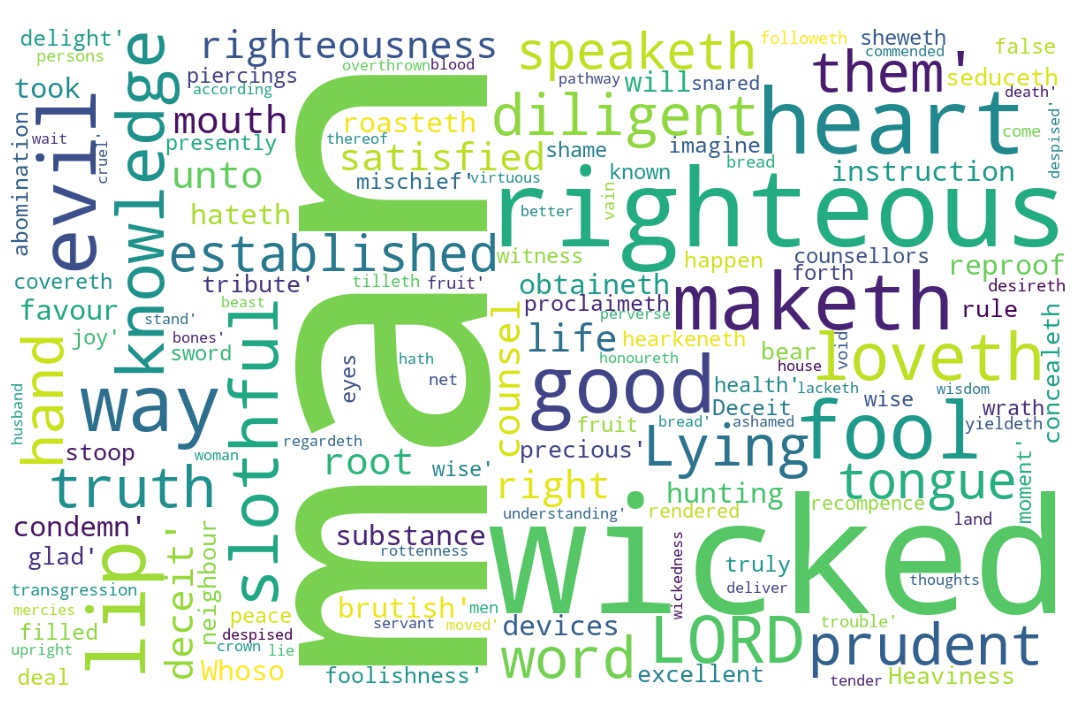
\includegraphics[width=\linewidth]{20OT-Proverbs/Proverb12-WordCloud.jpg}
  \caption{Proverb 12 Word Cloud}
  \label{fig:Proverb 12 Word Cloud}
\end{figure}

\marginpar{\scriptsize \centering \fcolorbox{bone}{lime}{\textbf{SURE THINGS}}\\ (Proverb 12:1-27) \begin{compactenum}[I.][8]
    \item \textbf{Contented Man} \index[scripture]{Proverbs!Pro 12:01}(Pro 12:1) 
    \item \textbf{Contentious Mate} \index[scripture]{Proverbs!Pro 12:04}(Pro 12:4) 
    \item \textbf{Commended Man} \index[scripture]{Proverbs!Pro 12:08}(Pro 12:8) 
    \item \textbf{Condemned Man} \index[scripture]{Proverbs!Pro 12:09}(Pro 12:9) 
    \item \textbf{Correct Mouth} \index[scripture]{Proverbs!Pro 12:17}(Pro 12:17) 
    \item \textbf{Continual Misery} \index[scripture]{Proverbs!Pro 12:25}(Pro 12:25) 
    \item \textbf{Comforting Materials} \index[scripture]{Proverbs!Pro 12:27}(Pro 12:27) 
\end{compactenum}}

\marginpar{\scriptsize \centering \fcolorbox{bone}{yellow}{\textbf{WICKED WAYS \& WORDS}}\\ (Proverb 12:1-27) \begin{compactenum}[I.][8]
    \item They do not Provide \textbf{Security} \index[scripture]{Proverbs!Pro 12:03}(Pro 12:3) 
    \item They do not Provide \textbf{Satisfaction} \index[scripture]{Proverbs!Pro 12:11}\index[scripture]{Proverbs!Pro 12:14}(Pro 12:11, 14) 
    \item They are \textbf{Snares} \index[scripture]{Proverbs!Pro 12:13}(Pro 12:13) 
    \item They lead to \textbf{Shame} \index[scripture]{Proverbs!Pro 12:16}(Pro 12:16) 
    \item They Pierce like a \textbf{Sword} \index[scripture]{Proverbs!Pro 12:18}(Pro 12:18) 
    \item They Produce \textbf{Slothfulness and Servanthood} \index[scripture]{Proverbs!Pro 12:24}\index[scripture]{Proverbs!Pro 12:27}(Prov 12:24, 27) 
\end{compactenum}}

\marginpar{\scriptsize \centering \fcolorbox{bone}{black}{\textbf{\textcolor[cmyk]{0,0,0,0}{PARTS OF LIFE}}}\\ (Proverb 12:1-27) 
 \begin{compactenum}[I.][8]
    \item \textbf{Path to Growth} \index[scripture]{Proverbs!Pro 12:01}(Pro 12:1) 
    \item \textbf{Promise of God} \index[scripture]{Proverbs!Pro 12:02} (Pro 12:2) 
    \item \textbf{Perennial Aggravation} \index[scripture]{Proverbs!Pro 12:04}(Pro 12:04)
    \item \textbf{Perverse Goals} \index[scripture]{Proverbs!Pro 12:08}(Pro 12:08) 
    \item \textbf{Presence of Grief} \index[scripture]{Proverbs!Pro 12:08}(Pro 12:08)
    \item \textbf{Practical Regard} \index[scripture]{Proverbs!Pro 12:10}(Pro 12:10) 
    \item \textbf{Pattern of Goodness} \index[scripture]{Proverbs!Pro 12:24}(Pro 12:24) 
\end{compactenum}}


\marginpar{\scriptsize \centering \fcolorbox{bone}{blue}{\textbf{\textcolor[cmyk]{0,0,0,0}{A VIRTUOUS WOMAN}}}\\ (Proverb 12:1-27) 
 \begin{compactenum}[I.][8]
    \item \textbf{Correctable} \index[scripture]{Proverbs!Pro 12:04}(Pro 12:4) 
    \item \textbf{Conformable} \index[scripture]{Proverbs!Pro 12:04}(Pro 12:4) 
    \item \textbf{Cooperative} \index[scripture]{Proverbs!Pro 12:04}(Pro 12:4) 
    \item \textbf{Calm} \index[scripture]{Proverbs!Pro 12:04}(Pro 12:4) 
    \item A \textbf{Crown} \index[scripture]{Proverbs!Pro 12:04}(Pro 12:4) 
    \item \textbf{Caring} \index[scripture]{Proverbs!Pro 12:04}(Pro 12:4) 
    \item \textbf{Considerate} \index[scripture]{Proverbs!Pro 12:04}(Pro 12:4) 
\end{compactenum}}

\marginpar{\scriptsize \centering \fcolorbox{bone}{orange}{\textbf{THE EXAMINATION}}\\ (Proverb 12:1-27) \begin{compactenum}[I.][8]
    \item What their \textbf{Hearts} Love \index[scripture]{Proverbs!Pro 12:01}(Pro 12:1) 
    \item What Their \textbf{Hands} Produce \index[scripture]{Proverbs!Pro 12:04}(Pro 12:4) 
    \item \textbf{How} they treat the Helpless \index[scripture]{Proverbs!Pro 12:08}(Pro 12:8) 
    \item The \textbf{Health} of Their speech \index[scripture]{Proverbs!Pro 12:181}(Pro 12:8) 
    \item What he \textbf{Hearkened} to \index[scripture]{Proverbs!Pro 12:15}(Pro 12:15) 
    \item What is \textbf{Honoured} to \index[scripture]{Proverbs!Pro 12:09}(Pro 12:9) 
    \item How they \textbf{Handle} the Details
    \index[scripture]{Proverbs!Pro 12:09}(Pro 12:9) 
\end{compactenum}}

%%%%%%%%%%%%%%%%%%%%%%%%%%%%%%%%%%
%%%%%%%%%%%%%%%%%%%%%%%%%%%%%%%%%
\footnote{\textcolor[cmyk]{0.99998,1,0,0}{\hyperlink{TOC}{Return to end of Table of Contents.}}}\footnote{\href{https://audiobible.com/bible/proverbs_12.html}{\textcolor[cmyk]{0.99998,1,0,0}{Proverbs Audio}}}\textcolor[cmyk]{0.99998,1,0,0}{Whoso \fcolorbox{bone}{lime}{loveth instruction} loveth \fcolorbox{bone}{blue}{\textbf{\textcolor[cmyk]{0,0,0,0}{knowledge}}}: but he that hateth reproof \emph{is} brutish.}
[2] \textcolor[cmyk]{0.99998,1,0,0}{A good \emph{man} obtaineth \fcolorbox{bone}{lime}{favour of} \fcolorbox{bone}{blue}{\textbf{\textcolor[cmyk]{0,0,0,0}{the LORD}}}: but \fcolorbox{bone}{bone}{a} man of wicked devices will he condemn.}
[3] \textcolor[cmyk]{0.99998,1,0,0}{A man shall \fcolorbox{bone}{yellow}{not be}  \fcolorbox{bone}{yellow}{established} by wickedness: but the root of the righteous shall not be moved.}
[4] \textcolor[cmyk]{0.99998,1,0,0}{A virtuous woman \emph{is} \fcolorbox{bone}{bone}{a} crown to her husband: but she that maketh ashamed \emph{is} as \fcolorbox{bone}{blue}{\textbf{\textcolor[cmyk]{0,0,0,0}{rottenness in his bones}}}.}
[5] \textcolor[cmyk]{0.99998,1,0,0}{The thoughts of the righteous \emph{are} right: \emph{but} the counsels of the wicked \emph{are} deceit.}
[6] \textcolor[cmyk]{0.99998,1,0,0}{The words of the wicked \emph{are} to lie in wait for blood: but the mouth of the upright shall deliver them.}
[7] \textcolor[cmyk]{0.99998,1,0,0}{The wicked are overthrown, and \emph{are} not: but the house of the righteous shall stand.}
[8] \textcolor[cmyk]{0.99998,1,0,0}{A man shall be \fcolorbox{bone}{lime}{commended} according to his wisdom: but he that is of \fcolorbox{bone}{bone}{a} \fcolorbox{bone}{blue}{\textbf{\textcolor[cmyk]{0,0,0,0}{perverse}}} heart shall be despised.}
[9] \textcolor[cmyk]{0.99998,1,0,0}{\emph{He} \emph{that} \emph{is} \fcolorbox{bone}{lime}{despised}, and hath \fcolorbox{bone}{bone}{a} servant, \emph{is} better than he that honoureth himself, and lacketh bread.}
[10] \textcolor[cmyk]{0.99998,1,0,0}{A righteous \emph{man} \fcolorbox{bone}{blue}{\textbf{\textcolor[cmyk]{0,0,0,0}{regardeth}}} the life of his beast: but the tender mercies of the wicked \emph{are} cruel.}
[11] \textcolor[cmyk]{0.99998,1,0,0}{He that tilleth his land shall be \fcolorbox{bone}{yellow}{satisfied} with bread: but he that followeth vain \emph{persons} \emph{is} void of \fcolorbox{bone}{MYGOLD}{understanding}.}
[12] \textcolor[cmyk]{0.99998,1,0,0}{The wicked desireth the net of evil \emph{men}: but the root of the righteous yieldeth \emph{fruit}.}
[13] \textcolor[cmyk]{0.99998,1,0,0}{The wicked is \fcolorbox{bone}{yellow}{snared} by the \fcolorbox{bone}{MYGOLD}{transgression} of \emph{his} lips: but the just shall come out of trouble.}\footnote{\textbf{Ecclesiastes 9:12} - For man also knoweth not his time: as the fishes that are taken in an evil net, and as the birds that are caught in the snare; so are the sons of men snared in an evil time, when it falleth suddenly upon them.}\footnote{\textbf{Isaiah 28:13} - But the word of the LORD was unto them precept upon precept, precept upon precept; line upon line, line upon line; here a little, and there a little; that they might go, and fall backward, and be broken, and snared, and taken.}\footnote{\textbf{Isaiah 42:22} - But this is a people robbed and spoiled; they are all of them snared in holes, and they are hid in prison houses: they are for a prey, and none delivereth; for a spoil, and none saith, Restore.}
[14] \textcolor[cmyk]{0.99998,1,0,0}{A man shall be satisfied with good by the fruit of \emph{his} mouth: and the recompence of \fcolorbox{bone}{bone}{a} man's hands shall be rendered unto him.}
[15] \textcolor[cmyk]{0.99998,1,0,0}{The way of \fcolorbox{bone}{bone}{a} fool \emph{is} right in his own eyes: but he that hearkeneth unto counsel \emph{is} wise.}
[16] \textcolor[cmyk]{0.99998,1,0,0}{A fool's wrath is presently known: but \fcolorbox{bone}{bone}{a} prudent \emph{man} covereth \fcolorbox{bone}{yellow}{shame}.}\footnote{\textbf{Proverb 27:3}  -  A stone is heavy, and the sand weighty; but a fool’s wrath is heavier than them both.}
[17] \textcolor[cmyk]{0.99998,1,0,0}{\emph{He} \emph{that} \fcolorbox{bone}{lime}{speaketh truth} sheweth forth \fcolorbox{bone}{MYGOLD}{righteousness}: but \fcolorbox{bone}{bone}{a} false witness deceit.}
[18] \textcolor[cmyk]{0.99998,1,0,0}{There is that speaketh like the piercings of \fcolorbox{bone}{bone}{a} \fcolorbox{bone}{yellow}{sword}: but the tongue of the wise \emph{is} health.}
[19] \textcolor[cmyk]{0.99998,1,0,0}{The lip of truth shall be established for ever: but \fcolorbox{bone}{bone}{a} lying tongue \emph{is} but for \fcolorbox{bone}{bone}{a} moment.}
[20] \textcolor[cmyk]{0.99998,1,0,0}{Deceit \emph{is} in the heart of them that imagine evil: but to the counsellors of peace \emph{is} joy.}
[21] \textcolor[cmyk]{0.99998,1,0,0}{There shall no evil happen to the just: but the wicked shall be filled with mischief.}
[22] \textcolor[cmyk]{0.99998,1,0,0}{Lying lips \emph{are} abomination to the LORD: but they that deal truly \emph{are} his delight.}
[23] \textcolor[cmyk]{0.99998,1,0,0}{A prudent man concealeth knowledge: but the heart of fools proclaimeth foolishness.}
[24] \textcolor[cmyk]{0.99998,1,0,0}{\fcolorbox{bone}{blue}{\textbf{\textcolor[cmyk]{0,0,0,0}{The hand of the diligent}}} shall bear rule: but the \fcolorbox{bone}{yellow}{slothful} shall be under \fcolorbox{bone}{yellow}{tribute.}}
[25] \textcolor[cmyk]{0.99998,1,0,0}{\fcolorbox{bone}{lime}{Heaviness} in the heart of man maketh it stoop: but \fcolorbox{bone}{bone}{a} good word maketh it glad.}
[26] \textcolor[cmyk]{0.99998,1,0,0}{The righteous \emph{is} more excellent than his neighbour: but the way of the wicked seduceth them.}
[27] \textcolor[cmyk]{0.99998,1,0,0}{The \fcolorbox{bone}{yellow}{slothful} \emph{man} roasteth not that which he took in hunting: but the substance of \fcolorbox{bone}{bone}{a} diligent man \emph{is} \fcolorbox{bone}{lime}{precious}.}
[28] \textcolor[cmyk]{0.99998,1,0,0}{In the way of \fcolorbox{bone}{MYGOLD}{righteousness} \emph{is} life; and \emph{in} the pathway \emph{thereof} \emph{there} \emph{is} no death.}\footnote{\textbf{Psalm 1:1, 6} - Blessed is the man that walketh not in the counsel of the ungodly, nor standeth in the way of sinners, nor sitteth in the seat of the scornful. [6] For the LORD knoweth the way of the righteous: but the way of the ungodly shall perish.}





\index[NWIV]{12!Proverbs!Pro 12:1}\index[AWIP]{Whoso!Proverbs!Pro 12:1}\index[AWIP]{loveth!Proverbs!Pro 12:1}\index[AWIP]{loveth!Proverbs!Pro 12:1 (2)}\index[AWIP]{instruction!Proverbs!Pro 12:1}\index[AWIP]{knowledge!Proverbs!Pro 12:1}\index[AWIP]{but!Proverbs!Pro 12:1}\index[AWIP]{he!Proverbs!Pro 12:1}\index[AWIP]{that!Proverbs!Pro 12:1}\index[AWIP]{hateth!Proverbs!Pro 12:1}\index[AWIP]{reproof!Proverbs!Pro 12:1}\index[AWIP]{\emph{is}!Proverbs!Pro 12:1}\index[AWIP]{brutish!Proverbs!Pro 12:1}\index[AWIP]{\emph{is}!Proverbs!Pro 12:1}

\index[NWIV]{17!Proverbs!Pro 12:2}\index[AWIP]{A!Proverbs!Pro 12:2}\index[AWIP]{good!Proverbs!Pro 12:2}\index[AWIP]{\emph{man}!Proverbs!Pro 12:2}\index[AWIP]{obtaineth!Proverbs!Pro 12:2}\index[AWIP]{favour!Proverbs!Pro 12:2}\index[AWIP]{of!Proverbs!Pro 12:2}\index[AWIP]{of!Proverbs!Pro 12:2 (2)}\index[AWIP]{the!Proverbs!Pro 12:2}\index[AWIP]{LORD!Proverbs!Pro 12:2}\index[AWIP]{but!Proverbs!Pro 12:2}\index[AWIP]{a!Proverbs!Pro 12:2}\index[AWIP]{man!Proverbs!Pro 12:2}\index[AWIP]{wicked!Proverbs!Pro 12:2}\index[AWIP]{devices!Proverbs!Pro 12:2}\index[AWIP]{will!Proverbs!Pro 12:2}\index[AWIP]{he!Proverbs!Pro 12:2}\index[AWIP]{condemn!Proverbs!Pro 12:2}\index[AWIP]{\emph{man}!Proverbs!Pro 12:2}

\index[NWIV]{18!Proverbs!Pro 12:3}\index[AWIP]{A!Proverbs!Pro 12:3}\index[AWIP]{man!Proverbs!Pro 12:3}\index[AWIP]{shall!Proverbs!Pro 12:3}\index[AWIP]{shall!Proverbs!Pro 12:3 (2)}\index[AWIP]{not!Proverbs!Pro 12:3}\index[AWIP]{not!Proverbs!Pro 12:3 (2)}\index[AWIP]{be!Proverbs!Pro 12:3}\index[AWIP]{be!Proverbs!Pro 12:3 (2)}\index[AWIP]{established!Proverbs!Pro 12:3}\index[AWIP]{by!Proverbs!Pro 12:3}\index[AWIP]{wickedness!Proverbs!Pro 12:3}\index[AWIP]{but!Proverbs!Pro 12:3}\index[AWIP]{the!Proverbs!Pro 12:3}\index[AWIP]{the!Proverbs!Pro 12:3 (2)}\index[AWIP]{root!Proverbs!Pro 12:3}\index[AWIP]{of!Proverbs!Pro 12:3}\index[AWIP]{righteous!Proverbs!Pro 12:3}\index[AWIP]{moved!Proverbs!Pro 12:3}

\index[NWIV]{20!Proverbs!Pro 12:4}\index[AWIP]{A!Proverbs!Pro 12:4}\index[AWIP]{virtuous!Proverbs!Pro 12:4}\index[AWIP]{woman!Proverbs!Pro 12:4}\index[AWIP]{\emph{is}!Proverbs!Pro 12:4}\index[AWIP]{\emph{is}!Proverbs!Pro 12:4 (2)}\index[AWIP]{a!Proverbs!Pro 12:4}\index[AWIP]{crown!Proverbs!Pro 12:4}\index[AWIP]{to!Proverbs!Pro 12:4}\index[AWIP]{her!Proverbs!Pro 12:4}\index[AWIP]{husband!Proverbs!Pro 12:4}\index[AWIP]{but!Proverbs!Pro 12:4}\index[AWIP]{she!Proverbs!Pro 12:4}\index[AWIP]{that!Proverbs!Pro 12:4}\index[AWIP]{maketh!Proverbs!Pro 12:4}\index[AWIP]{ashamed!Proverbs!Pro 12:4}\index[AWIP]{as!Proverbs!Pro 12:4}\index[AWIP]{rottenness!Proverbs!Pro 12:4}\index[AWIP]{in!Proverbs!Pro 12:4}\index[AWIP]{his!Proverbs!Pro 12:4}\index[AWIP]{bones!Proverbs!Pro 12:4}\index[AWIP]{\emph{is}!Proverbs!Pro 12:4}\index[AWIP]{\emph{is}!Proverbs!Pro 12:4 (2)}

\index[NWIV]{15!Proverbs!Pro 12:5}\index[AWIP]{The!Proverbs!Pro 12:5}\index[AWIP]{thoughts!Proverbs!Pro 12:5}\index[AWIP]{of!Proverbs!Pro 12:5}\index[AWIP]{of!Proverbs!Pro 12:5 (2)}\index[AWIP]{the!Proverbs!Pro 12:5}\index[AWIP]{the!Proverbs!Pro 12:5 (2)}\index[AWIP]{the!Proverbs!Pro 12:5 (3)}\index[AWIP]{righteous!Proverbs!Pro 12:5}\index[AWIP]{\emph{are}!Proverbs!Pro 12:5}\index[AWIP]{\emph{are}!Proverbs!Pro 12:5 (2)}\index[AWIP]{right!Proverbs!Pro 12:5}\index[AWIP]{\emph{but}!Proverbs!Pro 12:5}\index[AWIP]{counsels!Proverbs!Pro 12:5}\index[AWIP]{wicked!Proverbs!Pro 12:5}\index[AWIP]{deceit!Proverbs!Pro 12:5}\index[AWIP]{\emph{are}!Proverbs!Pro 12:5}\index[AWIP]{\emph{are}!Proverbs!Pro 12:5 (2)}\index[AWIP]{\emph{but}!Proverbs!Pro 12:5}

\index[NWIV]{21!Proverbs!Pro 12:6}\index[AWIP]{The!Proverbs!Pro 12:6}\index[AWIP]{words!Proverbs!Pro 12:6}\index[AWIP]{of!Proverbs!Pro 12:6}\index[AWIP]{of!Proverbs!Pro 12:6 (2)}\index[AWIP]{the!Proverbs!Pro 12:6}\index[AWIP]{the!Proverbs!Pro 12:6 (2)}\index[AWIP]{the!Proverbs!Pro 12:6 (3)}\index[AWIP]{wicked!Proverbs!Pro 12:6}\index[AWIP]{\emph{are}!Proverbs!Pro 12:6}\index[AWIP]{to!Proverbs!Pro 12:6}\index[AWIP]{lie!Proverbs!Pro 12:6}\index[AWIP]{in!Proverbs!Pro 12:6}\index[AWIP]{wait!Proverbs!Pro 12:6}\index[AWIP]{for!Proverbs!Pro 12:6}\index[AWIP]{blood!Proverbs!Pro 12:6}\index[AWIP]{but!Proverbs!Pro 12:6}\index[AWIP]{mouth!Proverbs!Pro 12:6}\index[AWIP]{upright!Proverbs!Pro 12:6}\index[AWIP]{shall!Proverbs!Pro 12:6}\index[AWIP]{deliver!Proverbs!Pro 12:6}\index[AWIP]{them!Proverbs!Pro 12:6}\index[AWIP]{\emph{are}!Proverbs!Pro 12:6}

\index[NWIV]{15!Proverbs!Pro 12:7}\index[AWIP]{The!Proverbs!Pro 12:7}\index[AWIP]{wicked!Proverbs!Pro 12:7}\index[AWIP]{are!Proverbs!Pro 12:7}\index[AWIP]{overthrown!Proverbs!Pro 12:7}\index[AWIP]{and!Proverbs!Pro 12:7}\index[AWIP]{\emph{are}!Proverbs!Pro 12:7}\index[AWIP]{not!Proverbs!Pro 12:7}\index[AWIP]{but!Proverbs!Pro 12:7}\index[AWIP]{the!Proverbs!Pro 12:7}\index[AWIP]{the!Proverbs!Pro 12:7 (2)}\index[AWIP]{house!Proverbs!Pro 12:7}\index[AWIP]{of!Proverbs!Pro 12:7}\index[AWIP]{righteous!Proverbs!Pro 12:7}\index[AWIP]{shall!Proverbs!Pro 12:7}\index[AWIP]{stand!Proverbs!Pro 12:7}\index[AWIP]{\emph{are}!Proverbs!Pro 12:7}

\index[NWIV]{20!Proverbs!Pro 12:8}\index[AWIP]{A!Proverbs!Pro 12:8}\index[AWIP]{man!Proverbs!Pro 12:8}\index[AWIP]{shall!Proverbs!Pro 12:8}\index[AWIP]{shall!Proverbs!Pro 12:8 (2)}\index[AWIP]{be!Proverbs!Pro 12:8}\index[AWIP]{be!Proverbs!Pro 12:8 (2)}\index[AWIP]{commended!Proverbs!Pro 12:8}\index[AWIP]{according!Proverbs!Pro 12:8}\index[AWIP]{to!Proverbs!Pro 12:8}\index[AWIP]{his!Proverbs!Pro 12:8}\index[AWIP]{wisdom!Proverbs!Pro 12:8}\index[AWIP]{but!Proverbs!Pro 12:8}\index[AWIP]{he!Proverbs!Pro 12:8}\index[AWIP]{that!Proverbs!Pro 12:8}\index[AWIP]{is!Proverbs!Pro 12:8}\index[AWIP]{of!Proverbs!Pro 12:8}\index[AWIP]{a!Proverbs!Pro 12:8}\index[AWIP]{perverse!Proverbs!Pro 12:8}\index[AWIP]{heart!Proverbs!Pro 12:8}\index[AWIP]{despised!Proverbs!Pro 12:8}

\index[NWIV]{18!Proverbs!Pro 12:9}\index[AWIP]{\emph{He}!Proverbs!Pro 12:9}\index[AWIP]{\emph{that}!Proverbs!Pro 12:9}\index[AWIP]{\emph{is}!Proverbs!Pro 12:9}\index[AWIP]{\emph{is}!Proverbs!Pro 12:9 (2)}\index[AWIP]{despised!Proverbs!Pro 12:9}\index[AWIP]{and!Proverbs!Pro 12:9}\index[AWIP]{and!Proverbs!Pro 12:9 (2)}\index[AWIP]{hath!Proverbs!Pro 12:9}\index[AWIP]{a!Proverbs!Pro 12:9}\index[AWIP]{servant!Proverbs!Pro 12:9}\index[AWIP]{better!Proverbs!Pro 12:9}\index[AWIP]{than!Proverbs!Pro 12:9}\index[AWIP]{he!Proverbs!Pro 12:9}\index[AWIP]{that!Proverbs!Pro 12:9}\index[AWIP]{honoureth!Proverbs!Pro 12:9}\index[AWIP]{himself!Proverbs!Pro 12:9}\index[AWIP]{lacketh!Proverbs!Pro 12:9}\index[AWIP]{bread!Proverbs!Pro 12:9}\index[AWIP]{\emph{He}!Proverbs!Pro 12:9}\index[AWIP]{\emph{that}!Proverbs!Pro 12:9}\index[AWIP]{\emph{is}!Proverbs!Pro 12:9}\index[AWIP]{\emph{is}!Proverbs!Pro 12:9 (2)}

\index[NWIV]{18!Proverbs!Pro 12:10}\index[AWIP]{A!Proverbs!Pro 12:10}\index[AWIP]{righteous!Proverbs!Pro 12:10}\index[AWIP]{\emph{man}!Proverbs!Pro 12:10}\index[AWIP]{regardeth!Proverbs!Pro 12:10}\index[AWIP]{the!Proverbs!Pro 12:10}\index[AWIP]{the!Proverbs!Pro 12:10 (2)}\index[AWIP]{the!Proverbs!Pro 12:10 (3)}\index[AWIP]{life!Proverbs!Pro 12:10}\index[AWIP]{of!Proverbs!Pro 12:10}\index[AWIP]{of!Proverbs!Pro 12:10 (2)}\index[AWIP]{his!Proverbs!Pro 12:10}\index[AWIP]{beast!Proverbs!Pro 12:10}\index[AWIP]{but!Proverbs!Pro 12:10}\index[AWIP]{tender!Proverbs!Pro 12:10}\index[AWIP]{mercies!Proverbs!Pro 12:10}\index[AWIP]{wicked!Proverbs!Pro 12:10}\index[AWIP]{\emph{are}!Proverbs!Pro 12:10}\index[AWIP]{cruel!Proverbs!Pro 12:10}\index[AWIP]{\emph{man}!Proverbs!Pro 12:10}\index[AWIP]{\emph{are}!Proverbs!Pro 12:10}

\index[NWIV]{20!Proverbs!Pro 12:11}\index[AWIP]{He!Proverbs!Pro 12:11}\index[AWIP]{that!Proverbs!Pro 12:11}\index[AWIP]{that!Proverbs!Pro 12:11 (2)}\index[AWIP]{tilleth!Proverbs!Pro 12:11}\index[AWIP]{his!Proverbs!Pro 12:11}\index[AWIP]{land!Proverbs!Pro 12:11}\index[AWIP]{shall!Proverbs!Pro 12:11}\index[AWIP]{be!Proverbs!Pro 12:11}\index[AWIP]{satisfied!Proverbs!Pro 12:11}\index[AWIP]{with!Proverbs!Pro 12:11}\index[AWIP]{bread!Proverbs!Pro 12:11}\index[AWIP]{but!Proverbs!Pro 12:11}\index[AWIP]{he!Proverbs!Pro 12:11}\index[AWIP]{followeth!Proverbs!Pro 12:11}\index[AWIP]{vain!Proverbs!Pro 12:11}\index[AWIP]{\emph{persons}!Proverbs!Pro 12:11}\index[AWIP]{\emph{is}!Proverbs!Pro 12:11}\index[AWIP]{void!Proverbs!Pro 12:11}\index[AWIP]{of!Proverbs!Pro 12:11}\index[AWIP]{understanding!Proverbs!Pro 12:11}\index[AWIP]{\emph{persons}!Proverbs!Pro 12:11}\index[AWIP]{\emph{is}!Proverbs!Pro 12:11}

\index[NWIV]{16!Proverbs!Pro 12:12}\index[AWIP]{The!Proverbs!Pro 12:12}\index[AWIP]{wicked!Proverbs!Pro 12:12}\index[AWIP]{desireth!Proverbs!Pro 12:12}\index[AWIP]{the!Proverbs!Pro 12:12}\index[AWIP]{the!Proverbs!Pro 12:12 (2)}\index[AWIP]{the!Proverbs!Pro 12:12 (3)}\index[AWIP]{net!Proverbs!Pro 12:12}\index[AWIP]{of!Proverbs!Pro 12:12}\index[AWIP]{of!Proverbs!Pro 12:12 (2)}\index[AWIP]{evil!Proverbs!Pro 12:12}\index[AWIP]{\emph{men}!Proverbs!Pro 12:12}\index[AWIP]{but!Proverbs!Pro 12:12}\index[AWIP]{root!Proverbs!Pro 12:12}\index[AWIP]{righteous!Proverbs!Pro 12:12}\index[AWIP]{yieldeth!Proverbs!Pro 12:12}\index[AWIP]{\emph{fruit}!Proverbs!Pro 12:12}\index[AWIP]{\emph{men}!Proverbs!Pro 12:12}\index[AWIP]{\emph{fruit}!Proverbs!Pro 12:12}

\index[NWIV]{18!Proverbs!Pro 12:13}\index[AWIP]{The!Proverbs!Pro 12:13}\index[AWIP]{wicked!Proverbs!Pro 12:13}\index[AWIP]{is!Proverbs!Pro 12:13}\index[AWIP]{snared!Proverbs!Pro 12:13}\index[AWIP]{by!Proverbs!Pro 12:13}\index[AWIP]{the!Proverbs!Pro 12:13}\index[AWIP]{the!Proverbs!Pro 12:13 (2)}\index[AWIP]{transgression!Proverbs!Pro 12:13}\index[AWIP]{of!Proverbs!Pro 12:13}\index[AWIP]{of!Proverbs!Pro 12:13 (2)}\index[AWIP]{\emph{his}!Proverbs!Pro 12:13}\index[AWIP]{lips!Proverbs!Pro 12:13}\index[AWIP]{but!Proverbs!Pro 12:13}\index[AWIP]{just!Proverbs!Pro 12:13}\index[AWIP]{shall!Proverbs!Pro 12:13}\index[AWIP]{come!Proverbs!Pro 12:13}\index[AWIP]{out!Proverbs!Pro 12:13}\index[AWIP]{trouble!Proverbs!Pro 12:13}\index[AWIP]{\emph{his}!Proverbs!Pro 12:13}

\index[NWIV]{25!Proverbs!Pro 12:14}\index[AWIP]{A!Proverbs!Pro 12:14}\index[AWIP]{man!Proverbs!Pro 12:14}\index[AWIP]{shall!Proverbs!Pro 12:14}\index[AWIP]{shall!Proverbs!Pro 12:14 (2)}\index[AWIP]{be!Proverbs!Pro 12:14}\index[AWIP]{be!Proverbs!Pro 12:14 (2)}\index[AWIP]{satisfied!Proverbs!Pro 12:14}\index[AWIP]{with!Proverbs!Pro 12:14}\index[AWIP]{good!Proverbs!Pro 12:14}\index[AWIP]{by!Proverbs!Pro 12:14}\index[AWIP]{the!Proverbs!Pro 12:14}\index[AWIP]{the!Proverbs!Pro 12:14 (2)}\index[AWIP]{fruit!Proverbs!Pro 12:14}\index[AWIP]{of!Proverbs!Pro 12:14}\index[AWIP]{of!Proverbs!Pro 12:14 (2)}\index[AWIP]{\emph{his}!Proverbs!Pro 12:14}\index[AWIP]{mouth!Proverbs!Pro 12:14}\index[AWIP]{and!Proverbs!Pro 12:14}\index[AWIP]{recompence!Proverbs!Pro 12:14}\index[AWIP]{a!Proverbs!Pro 12:14}\index[AWIP]{man's!Proverbs!Pro 12:14}\index[AWIP]{hands!Proverbs!Pro 12:14}\index[AWIP]{rendered!Proverbs!Pro 12:14}\index[AWIP]{unto!Proverbs!Pro 12:14}\index[AWIP]{him!Proverbs!Pro 12:14}\index[AWIP]{\emph{his}!Proverbs!Pro 12:14}

\index[NWIV]{19!Proverbs!Pro 12:15}\index[AWIP]{The!Proverbs!Pro 12:15}\index[AWIP]{way!Proverbs!Pro 12:15}\index[AWIP]{of!Proverbs!Pro 12:15}\index[AWIP]{a!Proverbs!Pro 12:15}\index[AWIP]{fool!Proverbs!Pro 12:15}\index[AWIP]{\emph{is}!Proverbs!Pro 12:15}\index[AWIP]{\emph{is}!Proverbs!Pro 12:15 (2)}\index[AWIP]{right!Proverbs!Pro 12:15}\index[AWIP]{in!Proverbs!Pro 12:15}\index[AWIP]{his!Proverbs!Pro 12:15}\index[AWIP]{own!Proverbs!Pro 12:15}\index[AWIP]{eyes!Proverbs!Pro 12:15}\index[AWIP]{but!Proverbs!Pro 12:15}\index[AWIP]{he!Proverbs!Pro 12:15}\index[AWIP]{that!Proverbs!Pro 12:15}\index[AWIP]{hearkeneth!Proverbs!Pro 12:15}\index[AWIP]{unto!Proverbs!Pro 12:15}\index[AWIP]{counsel!Proverbs!Pro 12:15}\index[AWIP]{wise!Proverbs!Pro 12:15}\index[AWIP]{\emph{is}!Proverbs!Pro 12:15}\index[AWIP]{\emph{is}!Proverbs!Pro 12:15 (2)}

\index[NWIV]{12!Proverbs!Pro 12:16}\index[AWIP]{A!Proverbs!Pro 12:16}\index[AWIP]{fool's!Proverbs!Pro 12:16}\index[AWIP]{wrath!Proverbs!Pro 12:16}\index[AWIP]{is!Proverbs!Pro 12:16}\index[AWIP]{presently!Proverbs!Pro 12:16}\index[AWIP]{known!Proverbs!Pro 12:16}\index[AWIP]{but!Proverbs!Pro 12:16}\index[AWIP]{a!Proverbs!Pro 12:16}\index[AWIP]{prudent!Proverbs!Pro 12:16}\index[AWIP]{\emph{man}!Proverbs!Pro 12:16}\index[AWIP]{covereth!Proverbs!Pro 12:16}\index[AWIP]{shame!Proverbs!Pro 12:16}\index[AWIP]{\emph{man}!Proverbs!Pro 12:16}

\index[NWIV]{12!Proverbs!Pro 12:17}\index[AWIP]{\emph{He}!Proverbs!Pro 12:17}\index[AWIP]{\emph{that}!Proverbs!Pro 12:17}\index[AWIP]{speaketh!Proverbs!Pro 12:17}\index[AWIP]{truth!Proverbs!Pro 12:17}\index[AWIP]{sheweth!Proverbs!Pro 12:17}\index[AWIP]{forth!Proverbs!Pro 12:17}\index[AWIP]{righteousness!Proverbs!Pro 12:17}\index[AWIP]{but!Proverbs!Pro 12:17}\index[AWIP]{a!Proverbs!Pro 12:17}\index[AWIP]{false!Proverbs!Pro 12:17}\index[AWIP]{witness!Proverbs!Pro 12:17}\index[AWIP]{deceit!Proverbs!Pro 12:17}\index[AWIP]{\emph{He}!Proverbs!Pro 12:17}\index[AWIP]{\emph{that}!Proverbs!Pro 12:17}

\index[NWIV]{18!Proverbs!Pro 12:18}\index[AWIP]{There!Proverbs!Pro 12:18}\index[AWIP]{is!Proverbs!Pro 12:18}\index[AWIP]{that!Proverbs!Pro 12:18}\index[AWIP]{speaketh!Proverbs!Pro 12:18}\index[AWIP]{like!Proverbs!Pro 12:18}\index[AWIP]{the!Proverbs!Pro 12:18}\index[AWIP]{the!Proverbs!Pro 12:18 (2)}\index[AWIP]{the!Proverbs!Pro 12:18 (3)}\index[AWIP]{piercings!Proverbs!Pro 12:18}\index[AWIP]{of!Proverbs!Pro 12:18}\index[AWIP]{of!Proverbs!Pro 12:18 (2)}\index[AWIP]{a!Proverbs!Pro 12:18}\index[AWIP]{sword!Proverbs!Pro 12:18}\index[AWIP]{but!Proverbs!Pro 12:18}\index[AWIP]{tongue!Proverbs!Pro 12:18}\index[AWIP]{wise!Proverbs!Pro 12:18}\index[AWIP]{\emph{is}!Proverbs!Pro 12:18}\index[AWIP]{health!Proverbs!Pro 12:18}\index[AWIP]{\emph{is}!Proverbs!Pro 12:18}

\index[NWIV]{18!Proverbs!Pro 12:19}\index[AWIP]{The!Proverbs!Pro 12:19}\index[AWIP]{lip!Proverbs!Pro 12:19}\index[AWIP]{of!Proverbs!Pro 12:19}\index[AWIP]{truth!Proverbs!Pro 12:19}\index[AWIP]{shall!Proverbs!Pro 12:19}\index[AWIP]{be!Proverbs!Pro 12:19}\index[AWIP]{established!Proverbs!Pro 12:19}\index[AWIP]{for!Proverbs!Pro 12:19}\index[AWIP]{for!Proverbs!Pro 12:19 (2)}\index[AWIP]{ever!Proverbs!Pro 12:19}\index[AWIP]{but!Proverbs!Pro 12:19}\index[AWIP]{but!Proverbs!Pro 12:19 (2)}\index[AWIP]{a!Proverbs!Pro 12:19}\index[AWIP]{a!Proverbs!Pro 12:19 (2)}\index[AWIP]{lying!Proverbs!Pro 12:19}\index[AWIP]{tongue!Proverbs!Pro 12:19}\index[AWIP]{\emph{is}!Proverbs!Pro 12:19}\index[AWIP]{moment!Proverbs!Pro 12:19}\index[AWIP]{\emph{is}!Proverbs!Pro 12:19}

\index[NWIV]{18!Proverbs!Pro 12:20}\index[AWIP]{Deceit!Proverbs!Pro 12:20}\index[AWIP]{\emph{is}!Proverbs!Pro 12:20}\index[AWIP]{\emph{is}!Proverbs!Pro 12:20 (2)}\index[AWIP]{in!Proverbs!Pro 12:20}\index[AWIP]{the!Proverbs!Pro 12:20}\index[AWIP]{the!Proverbs!Pro 12:20 (2)}\index[AWIP]{heart!Proverbs!Pro 12:20}\index[AWIP]{of!Proverbs!Pro 12:20}\index[AWIP]{of!Proverbs!Pro 12:20 (2)}\index[AWIP]{them!Proverbs!Pro 12:20}\index[AWIP]{that!Proverbs!Pro 12:20}\index[AWIP]{imagine!Proverbs!Pro 12:20}\index[AWIP]{evil!Proverbs!Pro 12:20}\index[AWIP]{but!Proverbs!Pro 12:20}\index[AWIP]{to!Proverbs!Pro 12:20}\index[AWIP]{counsellors!Proverbs!Pro 12:20}\index[AWIP]{peace!Proverbs!Pro 12:20}\index[AWIP]{joy!Proverbs!Pro 12:20}\index[AWIP]{\emph{is}!Proverbs!Pro 12:20}\index[AWIP]{\emph{is}!Proverbs!Pro 12:20 (2)}

\index[NWIV]{16!Proverbs!Pro 12:21}\index[AWIP]{There!Proverbs!Pro 12:21}\index[AWIP]{shall!Proverbs!Pro 12:21}\index[AWIP]{shall!Proverbs!Pro 12:21 (2)}\index[AWIP]{no!Proverbs!Pro 12:21}\index[AWIP]{evil!Proverbs!Pro 12:21}\index[AWIP]{happen!Proverbs!Pro 12:21}\index[AWIP]{to!Proverbs!Pro 12:21}\index[AWIP]{the!Proverbs!Pro 12:21}\index[AWIP]{the!Proverbs!Pro 12:21 (2)}\index[AWIP]{just!Proverbs!Pro 12:21}\index[AWIP]{but!Proverbs!Pro 12:21}\index[AWIP]{wicked!Proverbs!Pro 12:21}\index[AWIP]{be!Proverbs!Pro 12:21}\index[AWIP]{filled!Proverbs!Pro 12:21}\index[AWIP]{with!Proverbs!Pro 12:21}\index[AWIP]{mischief!Proverbs!Pro 12:21}

\index[NWIV]{15!Proverbs!Pro 12:22}\index[AWIP]{Lying!Proverbs!Pro 12:22}\index[AWIP]{lips!Proverbs!Pro 12:22}\index[AWIP]{\emph{are}!Proverbs!Pro 12:22}\index[AWIP]{\emph{are}!Proverbs!Pro 12:22 (2)}\index[AWIP]{abomination!Proverbs!Pro 12:22}\index[AWIP]{to!Proverbs!Pro 12:22}\index[AWIP]{the!Proverbs!Pro 12:22}\index[AWIP]{LORD!Proverbs!Pro 12:22}\index[AWIP]{but!Proverbs!Pro 12:22}\index[AWIP]{they!Proverbs!Pro 12:22}\index[AWIP]{that!Proverbs!Pro 12:22}\index[AWIP]{deal!Proverbs!Pro 12:22}\index[AWIP]{truly!Proverbs!Pro 12:22}\index[AWIP]{his!Proverbs!Pro 12:22}\index[AWIP]{delight!Proverbs!Pro 12:22}\index[AWIP]{\emph{are}!Proverbs!Pro 12:22}\index[AWIP]{\emph{are}!Proverbs!Pro 12:22 (2)}

\index[NWIV]{12!Proverbs!Pro 12:23}\index[AWIP]{A!Proverbs!Pro 12:23}\index[AWIP]{prudent!Proverbs!Pro 12:23}\index[AWIP]{man!Proverbs!Pro 12:23}\index[AWIP]{concealeth!Proverbs!Pro 12:23}\index[AWIP]{knowledge!Proverbs!Pro 12:23}\index[AWIP]{but!Proverbs!Pro 12:23}\index[AWIP]{the!Proverbs!Pro 12:23}\index[AWIP]{heart!Proverbs!Pro 12:23}\index[AWIP]{of!Proverbs!Pro 12:23}\index[AWIP]{fools!Proverbs!Pro 12:23}\index[AWIP]{proclaimeth!Proverbs!Pro 12:23}\index[AWIP]{foolishness!Proverbs!Pro 12:23}

\index[NWIV]{15!Proverbs!Pro 12:24}\index[AWIP]{The!Proverbs!Pro 12:24}\index[AWIP]{hand!Proverbs!Pro 12:24}\index[AWIP]{of!Proverbs!Pro 12:24}\index[AWIP]{the!Proverbs!Pro 12:24}\index[AWIP]{the!Proverbs!Pro 12:24 (2)}\index[AWIP]{diligent!Proverbs!Pro 12:24}\index[AWIP]{shall!Proverbs!Pro 12:24}\index[AWIP]{shall!Proverbs!Pro 12:24 (2)}\index[AWIP]{bear!Proverbs!Pro 12:24}\index[AWIP]{rule!Proverbs!Pro 12:24}\index[AWIP]{but!Proverbs!Pro 12:24}\index[AWIP]{slothful!Proverbs!Pro 12:24}\index[AWIP]{be!Proverbs!Pro 12:24}\index[AWIP]{under!Proverbs!Pro 12:24}\index[AWIP]{tribute!Proverbs!Pro 12:24}

\index[NWIV]{16!Proverbs!Pro 12:25}\index[AWIP]{Heaviness!Proverbs!Pro 12:25}\index[AWIP]{in!Proverbs!Pro 12:25}\index[AWIP]{the!Proverbs!Pro 12:25}\index[AWIP]{heart!Proverbs!Pro 12:25}\index[AWIP]{of!Proverbs!Pro 12:25}\index[AWIP]{man!Proverbs!Pro 12:25}\index[AWIP]{maketh!Proverbs!Pro 12:25}\index[AWIP]{maketh!Proverbs!Pro 12:25 (2)}\index[AWIP]{it!Proverbs!Pro 12:25}\index[AWIP]{it!Proverbs!Pro 12:25 (2)}\index[AWIP]{stoop!Proverbs!Pro 12:25}\index[AWIP]{but!Proverbs!Pro 12:25}\index[AWIP]{a!Proverbs!Pro 12:25}\index[AWIP]{good!Proverbs!Pro 12:25}\index[AWIP]{word!Proverbs!Pro 12:25}\index[AWIP]{glad!Proverbs!Pro 12:25}

\index[NWIV]{16!Proverbs!Pro 12:26}\index[AWIP]{The!Proverbs!Pro 12:26}\index[AWIP]{righteous!Proverbs!Pro 12:26}\index[AWIP]{\emph{is}!Proverbs!Pro 12:26}\index[AWIP]{more!Proverbs!Pro 12:26}\index[AWIP]{excellent!Proverbs!Pro 12:26}\index[AWIP]{than!Proverbs!Pro 12:26}\index[AWIP]{his!Proverbs!Pro 12:26}\index[AWIP]{neighbour!Proverbs!Pro 12:26}\index[AWIP]{but!Proverbs!Pro 12:26}\index[AWIP]{the!Proverbs!Pro 12:26}\index[AWIP]{the!Proverbs!Pro 12:26 (2)}\index[AWIP]{way!Proverbs!Pro 12:26}\index[AWIP]{of!Proverbs!Pro 12:26}\index[AWIP]{wicked!Proverbs!Pro 12:26}\index[AWIP]{seduceth!Proverbs!Pro 12:26}\index[AWIP]{them!Proverbs!Pro 12:26}\index[AWIP]{\emph{is}!Proverbs!Pro 12:26}

\index[NWIV]{20!Proverbs!Pro 12:27}\index[AWIP]{The!Proverbs!Pro 12:27}\index[AWIP]{slothful!Proverbs!Pro 12:27}\index[AWIP]{\emph{man}!Proverbs!Pro 12:27}\index[AWIP]{roasteth!Proverbs!Pro 12:27}\index[AWIP]{not!Proverbs!Pro 12:27}\index[AWIP]{that!Proverbs!Pro 12:27}\index[AWIP]{which!Proverbs!Pro 12:27}\index[AWIP]{he!Proverbs!Pro 12:27}\index[AWIP]{took!Proverbs!Pro 12:27}\index[AWIP]{in!Proverbs!Pro 12:27}\index[AWIP]{hunting!Proverbs!Pro 12:27}\index[AWIP]{but!Proverbs!Pro 12:27}\index[AWIP]{the!Proverbs!Pro 12:27}\index[AWIP]{substance!Proverbs!Pro 12:27}\index[AWIP]{of!Proverbs!Pro 12:27}\index[AWIP]{a!Proverbs!Pro 12:27}\index[AWIP]{diligent!Proverbs!Pro 12:27}\index[AWIP]{man!Proverbs!Pro 12:27}\index[AWIP]{\emph{is}!Proverbs!Pro 12:27}\index[AWIP]{precious!Proverbs!Pro 12:27}\index[AWIP]{\emph{man}!Proverbs!Pro 12:27}\index[AWIP]{\emph{is}!Proverbs!Pro 12:27}

\index[NWIV]{16!Proverbs!Pro 12:28}\index[AWIP]{In!Proverbs!Pro 12:28}\index[AWIP]{the!Proverbs!Pro 12:28}\index[AWIP]{the!Proverbs!Pro 12:28 (2)}\index[AWIP]{way!Proverbs!Pro 12:28}\index[AWIP]{of!Proverbs!Pro 12:28}\index[AWIP]{righteousness!Proverbs!Pro 12:28}\index[AWIP]{\emph{is}!Proverbs!Pro 12:28}\index[AWIP]{\emph{is}!Proverbs!Pro 12:28 (2)}\index[AWIP]{life!Proverbs!Pro 12:28}\index[AWIP]{and!Proverbs!Pro 12:28}\index[AWIP]{\emph{in}!Proverbs!Pro 12:28}\index[AWIP]{pathway!Proverbs!Pro 12:28}\index[AWIP]{\emph{thereof}!Proverbs!Pro 12:28}\index[AWIP]{\emph{there}!Proverbs!Pro 12:28}\index[AWIP]{no!Proverbs!Pro 12:28}\index[AWIP]{death!Proverbs!Pro 12:28}\index[AWIP]{\emph{is}!Proverbs!Pro 12:28}\index[AWIP]{\emph{is}!Proverbs!Pro 12:28 (2)}\index[AWIP]{\emph{in}!Proverbs!Pro 12:28}\index[AWIP]{\emph{thereof}!Proverbs!Pro 12:28}\index[AWIP]{\emph{there}!Proverbs!Pro 12:28}


\section{Proverbs 12 Outlines}

\subsection{My Outlines}

\subsubsection{Sure Things}
\textbf{Introduction: }Sure Things in Proverbs 12
\index[speaker]{Keith Anthony!Proverb 12 (Sure Things)}
\index[series]{Proverbs (Keith Anthony)!Pro 12 (Sure Things)}
\index[date]{2015/09/12!Proverb 12 (Sure Things) (Keith Anthony)}
\begin{compactenum}[I.]
    \item \textbf{Contented Man} \index[scripture]{Proverbs!Pro 12:01}(Pro 12:1) 
    \item \textbf{Contentious Mate} \index[scripture]{Proverbs!Pro 12:04}(Pro 12:4) 
    \item \textbf{Commended Man} \index[scripture]{Proverbs!Pro 12:08}(Pro 12:8) 
    \item \textbf{Condemned Man} \index[scripture]{Proverbs!Pro 12:09}(Pro 12:9) 
    \item \textbf{Correct Mouth} \index[scripture]{Proverbs!Pro 12:17}(Pro 12:17) 
    \item \textbf{Continual Misery} \index[scripture]{Proverbs!Pro 12:25}(Pro 12:25) 
    \item \textbf{Comforting Materials} \index[scripture]{Proverbs!Pro 12:27}(Pro 12:27) 
\end{compactenum}

\subsubsection{Wicked Ways \& Words}
\index[speaker]{Keith Anthony!Proverb 12 (Wicked Ways \& Words)}
\index[series]{Proverbs (Keith Anthony)!Pro 12 (Wicked Ways \& Words)}
\index[date]{2015/09/12!Proverb 12 (Wicked Ways \& Words) (Keith Anthony)}
\begin{compactenum}[I.][8]
    \item They do not Provide \textbf{Security} \index[scripture]{Proverbs!Pro 12:03}(Pro 12:3) 
    \item They do not Provide \textbf{Satisfaction} \index[scripture]{Proverbs!Pro 12:11}\index[scripture]{Proverbs!Pro 12:14}(Pro 12:11, 14) 
    \item They are \textbf{Snares} \index[scripture]{Proverbs!Pro 12:13}(Pro 12:13) 
    \item They lead to \textbf{Shame} \index[scripture]{Proverbs!Pro 12:16}(Pro 12:16) 
    \item They Pierce like a \textbf{Sword} \index[scripture]{Proverbs!Pro 12:18}(Pro 12:18) 
    \item They Produce \textbf{Slothfulness and Servanthood} \index[scripture]{Proverbs!Pro 12:24}\index[scripture]{Proverbs!Pro 12:27}(Prov 12:24, 27) 
\end{compactenum}



\subsubsection{Parts of Life in Proverbs 12}
\textbf{Introduction: }Parts of Life in Proverbs 12
\index[speaker]{Keith Anthony!Proverb 12 (Parts of Life in Proverbs 12)}
\index[series]{Proverbs (Keith Anthony)!Pro 12 (Parts of Life in Proverbs 12)}
\index[date]{2015/09/12!Proverb 12 (Parts of Life in Proverbs 12) (Keith Anthony)}
\begin{compactenum}[I.]
    \item \textbf{Path to Growth} \index[scripture]{Proverbs!Pro 12:01}(Pro 12:1) 
    \item \textbf{Promise of God} \index[scripture]{Proverbs!Pro 12:02} (Pro 12:2) 
    \item \textbf{Perennial Aggravation} \index[scripture]{Proverbs!Pro 12:04}(Pro 12:04)
    \item \textbf{Perverse Goals} \index[scripture]{Proverbs!Pro 12:08}(Pro 12:08) 
    \item \textbf{Presence of Grief} \index[scripture]{Proverbs!Pro 12:08}(Pro 12:08)
    \item \textbf{Practical Regard} \index[scripture]{Proverbs!Pro 12:10}(Pro 12:10) 
    \item \textbf{Pattern of Goodness} \index[scripture]{Proverbs!Pro 12:24}(Pro 12:24) 
\end{compactenum}

\subsubsection{Describing the Virtuous Woman}
\textbf{Introduction: }Describing the Virtuous Woman
\index[speaker]{Keith Anthony!Proverb 12 (Describing the Virtuous Woman)}
\index[series]{Proverbs (Keith Anthony)!Pro 12 (Describing the Virtuous Woman)}
\index[date]{2016/05/12!Proverb 12 (Describing the Virtuous Woman) (Keith Anthony)}
\begin{compactenum}[I.]
    \item \textbf{Correctable} \index[scripture]{Proverbs!Pro 12:04}(Pro 12:4) 
    \item \textbf{Conformable} \index[scripture]{Proverbs!Pro 12:04}(Pro 12:4) 
    \item \textbf{Cooperative} \index[scripture]{Proverbs!Pro 12:04}(Pro 12:4) 
    \item \textbf{Calm} \index[scripture]{Proverbs!Pro 12:04}(Pro 12:4) 
    \item A \textbf{Crown} \index[scripture]{Proverbs!Pro 12:04}(Pro 12:4) 
    \item \textbf{Caring} \index[scripture]{Proverbs!Pro 12:04}(Pro 12:4) 
    \item \textbf{Considerate} \index[scripture]{Proverbs!Pro 12:04}(Pro 12:4) 
\end{compactenum}

\subsubsection{Following Vain Persons}
%\footnote{12 May 2017, Keith Anthony}
\index[speaker]{Keith Anthony!Proverb 12:11 (Following Vain Persons)}
\index[series]{Proverbs (Keith Anthony)!Pro 12:11 (Following Vain Persons)}
\index[date]{2017/05/12!Proverb 12:11 (Following Vain Persons) (Keith Anthony)}
\textbf{Introduction: }Why are they being Followed:
\begin{compactenum}[I.]
    \item Their \textbf{Promises} \index[scripture]{Proverbs!Pro 12:11}(Pro 12:11) 
    \item Their \textbf{Popularity} \index[scripture]{Proverbs!Pro 12:11}(Pro 12:11) 
    \item Their \textbf{Performance} \index[scripture]{Proverbs!Pro 12:11}(Pro 12:11) 
    \item Their \textbf{Presence} \index[scripture]{Proverbs!Pro 12:11}(Pro 12:11) 
    \item Their \textbf{Prevarications} \index[scripture]{Proverbs!Pro 12:11}(Pro 12:11) 
    \item Their \textbf{Presentation} \index[scripture]{Proverbs!Pro 12:11}(Pro 12:11) 
    \item Their \textbf{Promotion} \index[scripture]{Proverbs!Pro 12:11}(Pro 12:11) 
\end{compactenum}

\subsubsection{13 ``P'' words and sounds in Proverbs 12}
\textbf{Introduction: }More Stuff in Proverbs 12:

\index[speaker]{Keith Anthony!Proverb 12 (13 ``P'' words and sounds in Proverbs 12)}
\index[series]{Proverbs (Keith Anthony)!Pro 12 (13 ``P'' words and sounds in Proverbs 12)}
\index[date]{2015/09/12!Proverb 12 (13 ``P'' words and sounds in Proverbs 12) (Keith Anthony)}
\begin{compactenum}[I.]
    \item \textbf{Reproof} \index[scripture]{Proverbs!Pro 12:01}(Pro 12:1)
    \item \textbf{Upright} \index[scripture]{Proverbs!Pro 12:06}(Pro 12:6)
    \item \textbf{Perverse} \index[scripture]{Proverbs!Pro 12:08}(Pro 12:8)
    \item \textbf{Persons} \index[scripture]{Proverbs!Pro 12:11}(Pro 12:11)
    \item \textbf{Recompence} \index[scripture]{Proverbs!Pro 12:14}(Pro 12:14)
    \item \textbf{Presentl}y \index[scripture]{Proverbs!Pro 12:16}(Pro 12:16)
    \item \textbf{Prudent} \index[scripture]{Proverbs!Pro 12:16}(Pro 12:16) 
    \item \textbf{Piercings} \index[scripture]{Proverbs!Pro 12:18}(Pro 12:18) 
    \item \textbf{Peace} \index[scripture]{Proverbs!Pro 12:20}(Pro 12:20) 
    \item \textbf{Proclaimeth} \index[scripture]{Proverbs!Pro 12:23}(Pro 12:23)
    \item \textbf{Prudent} \index[scripture]{Proverbs!Pro 12:23}(Pro 12:23) 
    \item \textbf{Precious} \index[scripture]{Proverbs!Pro 12:27}(Pro 12:27) 
    \item \textbf{Pathway} \index[scripture]{Proverbs!Pro 12:28}(Pro 12:28)
\end{compactenum}



\subsubsection{The Examination}
\textbf{Introduction: } Although this is ice that is thin, Proverbs 12 gives us a sense to examine where others ``are'':

\index[speaker]{Keith Anthony!Proverb 12 (The Examination)}
\index[series]{Proverbs (Keith Anthony)!Pro 12 (The Examination)}
\index[date]{2021/06/12!Proverb 12 (The Examination) (Keith Anthony)}

\begin{compactenum}[I.][8]
    \item What their \textbf{Hearts} Love \index[scripture]{Proverbs!Pro 12:01}(Pro 12:1) 
    \item What Their \textbf{Hands} Produce \index[scripture]{Proverbs!Pro 12:04}(Pro 12:4) 
    \item \textbf{How} they treat the Helpless \index[scripture]{Proverbs!Pro 12:08}(Pro 12:8) 
    \item The \textbf{Health} of Their speech \index[scripture]{Proverbs!Pro 12:181}(Pro 12:8) 
    \item What he \textbf{Hearkened} to \index[scripture]{Proverbs!Pro 12:15}(Pro 12:15) 
    \item What is \textbf{Honoured} to \index[scripture]{Proverbs!Pro 12:09}(Pro 12:9) 
    \item How they \textbf{Handle} the Details
    \index[scripture]{Proverbs!Pro 12:09}(Pro 12:9) 
\end{compactenum}


\subsection{Outlines from Others}

\section{Proverb 12 Comments}

\section{Numeric Nuggets}
\textbf{13:} Verses 12 and 24 have 13 unique words. The 13-letter words ``understanding,'' ``transgression, '' and `righteousness'' are used in the chapter. The word ``a'' is used 13 times in the chapter.

\subsection{Proverb 12 Introduction}

\normalsize
\begin{longtable}{c|p{2.1in}|p{2.1in}}
\caption[Comparing Two Ways]{Comparing Two Ways} \label{table:Comparing Two Ways} \\ 
\hline \multicolumn{1}{|c|}{\textbf{vs}} & \multicolumn{1}{c|}{\textbf{The Good}} &
\multicolumn{1}{c|}{\textbf{The Bad}} \\ \hline 
\endfirsthead
 
\multicolumn{3}{c}
{{\bfseries \tablename\ \thetable{} -- continued from previous page}} \\ 
\hline \multicolumn{1}{|c|}{\textbf{vs}} & \multicolumn{1}{c|}{\textbf{The Good}} &
\multicolumn{1}{c|}{\textbf{The Bad}} \\ \hline 
\endhead
 
\hline \multicolumn{3}{|r|}{{Continued if needed}} \\ \hline
\endfoot
 
\hline \hline
\endlastfoot
1 & loves instruction & hateth reproof \\ \hline
2 & obtains favour from the Lord & is condemned \\ \hline
3 & shall not be moved & is not established by wickedness \\ \hline
4 & virtuous woman is a crown to her husband & she that maeth ashamed is rottenness in a husband's bones \\ \hline
5 & thoughts of the righteous are right & counsels of the wicked are deceit \\ \hline
6 & mouth of the upright shall deliver them & the words of the wicked are to wait for blood \\ \hline
7 & house of the righteous shall stand & the wicked are overthrown and are not \\ \hline
8 & a man is commended according to his wisdom & those of a perverse heart are despised \\ \hline
10 & regards the life of his beast & are cruel \\ \hline
11 & he that tilleth his land shall be satisfied with bread & follows vain persons \\ \hline
12 & the root of the righteous yieldeth bread & desire the net of evil men \\ \hline
13 & shall come out of trouble & snared by the trangression of his lips \\ \hline
15 & hearkeneth unto counsel & is right in his own eyes\\ \hline
16 & a prudent man covereth shame & a fool's wrath is preentky known \\ \hline
17 & He that speaketh truth sheweth forth righteousness & false witness shews deceit \\ \hline
23 & a prudent man concealeth knowledge & heart of fools proclaimeth foolishness. \\ \hline
24 & The hand of the diligent shall bear rule  & the slothful shall be under tribute \\ \hline
27 & the substance of a diligent man is precious  & The slothful man roasteth not that which he took in hunting \\ \hline
28 & the way of righteousness is life  & death\\ \hline

\end{longtable}

\subsection{Proverb 12:1}
Proverb 12 starts with the ``brute'' in verse 1 and ends with the ``way of righteousness'' in verse 28.
\subsubsection{Forms of the word ``brute"}
There are 13 occurrences of forms of the word ``brute'' in scripture. So, the word should be considered along with other words in the club of those found 13 times.

\begin{compactenum}
    \item \textbf{Psalm 49:10} For he seeth that wise men die, likewise the fool and the brutish person perish, and leave their wealth to others. (``brutish'' is the 13th word)
    \item \textbf{Psalm 92:6}  A brutish man knoweth not; neither doth a fool understand this.
    \item \textbf{Psalm 94:8} Understand, ye brutish among the people: and ye fools, when will ye be wise?
    \item \textbf{Proverb 12:1}  Whoso loveth instruction loveth knowledge: but he that hateth reproof is brutish.
    \item \textbf{Proverb 30:2} Surely I am more brutish than any man, and have not the understanding of a man.
    \item \textbf{Isaiah 19:11} Surely the princes of Zoan are fools, the counsel of the wise counsellors of Pharaoh is become brutish: how say ye unto Pharaoh, I am the son of the wise, the son of ancient kings?
    \item \textbf{Jeremiah 10:8} But they are altogether brutish and foolish: the stock is a doctrine of vanities.
    \item \textbf{Jeremiah 10:14} Every man is brutish in his knowledge: every founder is confounded by the graven image: for his molten image is falsehood, and there is no breath in them.
    \item \textbf{Jeremiah 10:21}  For the pastors are become brutish, and have not sought the LORD: therefore they shall not prosper, and all their flocks shall be scattered.
    \item \textbf{Jeremiah 51:17} Every man is brutish by his knowledge; every founder is confounded by the graven image: for his molten image is falsehood, and there is no breath in them.
    \item \textbf{Ezekiel 21:31} And I will pour out mine indignation upon thee, I will blow against thee in the fire of my wrath, and deliver thee into the hand of brutish men, and skilful to destroy.
    \item \textbf{2 Peter 2:12} But these, as natural brute beasts, made to be taken and destroyed, speak evil of the things that they understand not; and shall utterly perish in their own corruption;
    \item \textbf{Jude 1:10} But these speak evil of those things which they know not: but what they know naturally, as brute beasts, in those things they corrupt themselves.
\end{compactenum}

\subsection{Proverb 12:4}
The phrase ``virtuous woman'' is found only three times in scripture: once in Ruth 3:11, here, and in Proverb 31:10. So, we can take Ruth as the only Biblical example.\footnote{\textbf{Ruth 3:11} - And now, my daughter, fear not; I will do to thee all that thou requirest: for all the city of my people doth know that thou art a virtuous woman.}



\subsection{Proverb 12 Repeated Phrases}


%%%%%%%%%%
%%%%%%%%%%
\normalsize
 
\begin{center}
\begin{longtable}{|p{3.0in}|p{0.5in}|}
\caption[Proverb 12 Repeated Phrases]{Proverb 12 Repeated Phrases}\label{table:Repeated Phrases Proverb 12} \\
\hline \multicolumn{1}{|c|}{\textbf{Phrase}} & \multicolumn{1}{c|}{\textbf{Frequency}} \\ \hline 
\endfirsthead
 
\multicolumn{2}{c}
{{\bfseries \tablename\ \thetable{} -- continued from previous page}} \\  
\hline \multicolumn{1}{|c|}{\textbf{Phrase}} & \multicolumn{1}{c|}{\textbf{Frequency}} \\ \hline 
\endhead
 
\hline \multicolumn{2}{c}{{ }} \\ \hline
\endfoot 
of the & 12\\ \hline 
but the & 12\\ \hline 
shall be & 8\\ \hline 
he that & 5\\ \hline 
but a & 5\\ \hline 
the wicked & 5\\ \hline 
of a & 5\\ \hline 
but he & 4\\ \hline 
but he that & 4\\ \hline 
of the righteous & 4\\ \hline 
the righteous & 4\\ \hline 
of the wicked & 4\\ \hline 
A man & 3\\ \hline 
A man shall & 3\\ \hline 
man shall & 3\\ \hline 
of the wicked \emph{are} & 3\\ \hline 
the wicked \emph{are} & 3\\ \hline 
wicked \emph{are} & 3\\ \hline 
The wicked & 3\\ \hline 
way of & 3\\ \hline 
the heart & 3\\ \hline 
the heart of & 3\\ \hline 
heart of & 3\\ \hline 
to the & 3\\ \hline 
\end{longtable}
\end{center}



%%%%%%%%%%
%%%%%%%%%%



%\newpage
\section{Proverb 12 Statistics}

%%%%%%%%%%%%%%%%%%%%%%%%%%%
%%%%% Word Statistics
%%%%%%%%%%%%%%%%%%%%%%%%%%

\normalsize
\subsection{Chapter Word Statistics}


%%%%%%%%%%
%%%%%%%%%%
 
\begin{center}
\begin{longtable}{l|c|c|c|c}
\caption[Stats for Proverb 12]{Stats for Proverb 12} \label{table:Stats for Proverb 12} \\ 
\hline \multicolumn{1}{|c|}{\textbf{Verse(s)}} & \multicolumn{1}{|c|}{\textbf{Count}} & \multicolumn{1}{|c|}{\textbf{Unique}} & \multicolumn{1}{|c|}{\textbf{Italics}} & \multicolumn{1}{|c|}{\textbf{Uniq Italic}}  \\ \hline 
\endfirsthead
 
\multicolumn{5}{c}
{{\bfseries \tablename\ \thetable{} -- continued from previous page}} \\  
\hline \multicolumn{1}{|c|}{\textbf{Verse(s)}} & \multicolumn{1}{|c|}{\textbf{Count}} & \multicolumn{1}{|c|}{\textbf{Unique}} & \multicolumn{1}{|c|}{\textbf{Italics}} & \multicolumn{1}{|c|}{\textbf{Uniq Italic}}  \\ \hline 
\endhead
 
\hline \multicolumn{5}{|r|}{{Continued if needed}} \\ \hline
\endfoot 
1 & 12 & 11 & 1 & 1\\ \hline
2 & 17 & 16 & 1 & 1\\ \hline
3 & 18 & 14 & 0 & 0\\ \hline
4 & 20 & 19 & 2 & 1\\ \hline
5 & 15 & 11 & 3 & 2\\ \hline
6 & 21 & 18 & 1 & 1\\ \hline
7 & 15 & 14 & 1 & 1\\ \hline
8 & 20 & 18 & 0 & 0\\ \hline
9 & 18 & 16 & 4 & 3\\ \hline
10 & 18 & 15 & 2 & 2\\ \hline
11 & 20 & 19 & 2 & 2\\ \hline
12 & 16 & 13 & 2 & 2\\ \hline
13 & 18 & 16 & 1 & 1\\ \hline
14 & 25 & 21 & 1 & 1\\ \hline
15 & 19 & 18 & 2 & 1\\ \hline
16 & 12 & 12 & 1 & 1\\ \hline
17 & 12 & 12 & 2 & 2\\ \hline
18 & 18 & 15 & 1 & 1\\ \hline
19 & 18 & 15 & 1 & 1\\ \hline
20 & 18 & 15 & 2 & 1\\ \hline
21 & 16 & 14 & 0 & 0\\ \hline
22 & 15 & 14 & 2 & 1\\ \hline
23 & 12 & 12 & 0 & 0\\ \hline
24 & 15 & 13 & 0 & 0\\ \hline
25 & 16 & 14 & 0 & 0\\ \hline
26 & 16 & 15 & 1 & 1\\ \hline
27 & 20 & 20 & 2 & 2\\ \hline
28 & 16 & 14 & 5 & 4\\ \hline
\hline \hline
Total & 476 & 201 & 40 & 13




\end{longtable}
\end{center}

%%%%%%%%%%
%%%%%%%%%%


\subsection{Words by Frequency}

\begin{center}
\begin{longtable}{l|r}
\caption[Word Frequencies in Proverb 12]{Word Frequencies in Proverb 12} \label{table:WordsIn-Proverb-12} \\ 
\hline \multicolumn{1}{|c|}{\textbf{Word}} & \multicolumn{1}{c|}{\textbf{Frequency}} \\ \hline 
\endfirsthead
  
\multicolumn{2}{c}  
{{\bfseries \tablename\ \thetable{} -- continued from previous page}} \\   
\hline \multicolumn{1}{|c|}{\textbf{Word}} & \multicolumn{1}{c|}{\textbf{Frequency}} \\ \hline   
\endhead  
  
\hline \multicolumn{2}{|r|}{{Continue}} \\ \hline  
\endfoot  
  
\hline \hline  
\endlastfoot  
  
the & 38\\ \hline 
of & 30\\ \hline 
but & 25\\ \hline 
\emph{is} & 16\\ \hline 
shall & 15\\ \hline 
a & 13\\ \hline 
that & 11\\ \hline 
be & 10\\ \hline 
The & 10\\ \hline 
wicked & 9\\ \hline 
A & 8\\ \hline 
he & 7\\ \hline 
man & 7\\ \hline 
his & 7\\ \hline 
\emph{are} & 7\\ \hline 
righteous & 6\\ \hline 
to & 6\\ \hline 
in & 6\\ \hline 
and & 5\\ \hline 
\emph{man} & 4\\ \hline 
not & 4\\ \hline 
is & 4\\ \hline 
heart & 4\\ \hline 
good & 3\\ \hline 
by & 3\\ \hline 
maketh & 3\\ \hline 
for & 3\\ \hline 
them & 3\\ \hline 
with & 3\\ \hline 
evil & 3\\ \hline 
way & 3\\ \hline 
loveth & 2\\ \hline 
knowledge & 2\\ \hline 
LORD & 2\\ \hline 
established & 2\\ \hline 
root & 2\\ \hline 
right & 2\\ \hline 
deceit & 2\\ \hline 
mouth & 2\\ \hline 
despised & 2\\ \hline 
\emph{He} & 2\\ \hline 
\emph{that} & 2\\ \hline 
than & 2\\ \hline 
bread & 2\\ \hline 
life & 2\\ \hline 
satisfied & 2\\ \hline 
\emph{his} & 2\\ \hline 
lips & 2\\ \hline 
just & 2\\ \hline 
unto & 2\\ \hline 
wise & 2\\ \hline 
prudent & 2\\ \hline 
speaketh & 2\\ \hline 
truth & 2\\ \hline 
righteousness & 2\\ \hline 
There & 2\\ \hline 
tongue & 2\\ \hline 
no & 2\\ \hline 
diligent & 2\\ \hline 
slothful & 2\\ \hline 
it & 2\\ \hline 
Whoso & 1\\ \hline 
instruction & 1\\ \hline 
hateth & 1\\ \hline 
reproof & 1\\ \hline 
brutish & 1\\ \hline 
obtaineth & 1\\ \hline 
favour & 1\\ \hline 
devices & 1\\ \hline 
will & 1\\ \hline 
condemn & 1\\ \hline 
wickedness & 1\\ \hline 
moved & 1\\ \hline 
virtuous & 1\\ \hline 
woman & 1\\ \hline 
crown & 1\\ \hline 
her & 1\\ \hline 
husband & 1\\ \hline 
she & 1\\ \hline 
ashamed & 1\\ \hline 
as & 1\\ \hline 
rottenness & 1\\ \hline 
bones & 1\\ \hline 
thoughts & 1\\ \hline 
\emph{but} & 1\\ \hline 
counsels & 1\\ \hline 
words & 1\\ \hline 
lie & 1\\ \hline 
wait & 1\\ \hline 
blood & 1\\ \hline 
upright & 1\\ \hline 
deliver & 1\\ \hline 
are & 1\\ \hline 
overthrown & 1\\ \hline 
house & 1\\ \hline 
stand & 1\\ \hline 
commended & 1\\ \hline 
according & 1\\ \hline 
wisdom & 1\\ \hline 
perverse & 1\\ \hline 
hath & 1\\ \hline 
servant & 1\\ \hline 
better & 1\\ \hline 
honoureth & 1\\ \hline 
himself & 1\\ \hline 
lacketh & 1\\ \hline 
regardeth & 1\\ \hline 
beast & 1\\ \hline 
tender & 1\\ \hline 
mercies & 1\\ \hline 
cruel & 1\\ \hline 
He & 1\\ \hline 
tilleth & 1\\ \hline 
land & 1\\ \hline 
followeth & 1\\ \hline 
vain & 1\\ \hline 
\emph{persons} & 1\\ \hline 
void & 1\\ \hline 
understanding & 1\\ \hline 
desireth & 1\\ \hline 
net & 1\\ \hline 
\emph{men} & 1\\ \hline 
yieldeth & 1\\ \hline 
\emph{fruit} & 1\\ \hline 
snared & 1\\ \hline 
transgression & 1\\ \hline 
come & 1\\ \hline 
out & 1\\ \hline 
trouble & 1\\ \hline 
fruit & 1\\ \hline 
recompence & 1\\ \hline 
man's & 1\\ \hline 
hands & 1\\ \hline 
rendered & 1\\ \hline 
him & 1\\ \hline 
fool & 1\\ \hline 
own & 1\\ \hline 
eyes & 1\\ \hline 
hearkeneth & 1\\ \hline 
counsel & 1\\ \hline 
fool's & 1\\ \hline 
wrath & 1\\ \hline 
presently & 1\\ \hline 
known & 1\\ \hline 
covereth & 1\\ \hline 
shame & 1\\ \hline 
sheweth & 1\\ \hline 
forth & 1\\ \hline 
false & 1\\ \hline 
witness & 1\\ \hline 
like & 1\\ \hline 
piercings & 1\\ \hline 
sword & 1\\ \hline 
health & 1\\ \hline 
lip & 1\\ \hline 
ever & 1\\ \hline 
lying & 1\\ \hline 
moment & 1\\ \hline 
Deceit & 1\\ \hline 
imagine & 1\\ \hline 
counsellors & 1\\ \hline 
peace & 1\\ \hline 
joy & 1\\ \hline 
happen & 1\\ \hline 
filled & 1\\ \hline 
mischief & 1\\ \hline 
Lying & 1\\ \hline 
abomination & 1\\ \hline 
they & 1\\ \hline 
deal & 1\\ \hline 
truly & 1\\ \hline 
delight & 1\\ \hline 
concealeth & 1\\ \hline 
fools & 1\\ \hline 
proclaimeth & 1\\ \hline 
foolishness & 1\\ \hline 
hand & 1\\ \hline 
bear & 1\\ \hline 
rule & 1\\ \hline 
under & 1\\ \hline 
tribute & 1\\ \hline 
Heaviness & 1\\ \hline 
stoop & 1\\ \hline 
word & 1\\ \hline 
glad & 1\\ \hline 
more & 1\\ \hline 
excellent & 1\\ \hline 
neighbour & 1\\ \hline 
seduceth & 1\\ \hline 
roasteth & 1\\ \hline 
which & 1\\ \hline 
took & 1\\ \hline 
hunting & 1\\ \hline 
substance & 1\\ \hline 
precious & 1\\ \hline 
In & 1\\ \hline 
\emph{in} & 1\\ \hline 
pathway & 1\\ \hline 
\emph{thereof} & 1\\ \hline 
\emph{there} & 1\\ \hline 
death & 1\\ \hline 
\end{longtable}  
\end{center}  


  
\normalsize  

  
  


\subsection{Words Alphabetically}

\begin{center}
\begin{longtable}{l|r}
\caption[Word Frequencies in Proverb 12]{Word Frequencies in Proverb 12} \label{table:WordsIn-Proverb-12} \\ 
\hline \multicolumn{1}{|c|}{\textbf{Word}} & \multicolumn{1}{c|}{\textbf{Frequency}} \\ \hline 
\endfirsthead
  
\multicolumn{2}{c}  
{{\bfseries \tablename\ \thetable{} -- continued from previous page}} \\   
\hline \multicolumn{1}{|c|}{\textbf{Word}} & \multicolumn{1}{c|}{\textbf{Frequency}} \\ \hline   
\endhead  
  
\hline \multicolumn{2}{|r|}{{Continue}} \\ \hline  
\endfoot  
  
\hline \hline  
\endlastfoot  
  
A & 8\\ \hline 
Deceit & 1\\ \hline 
He & 1\\ \hline 
Heaviness & 1\\ \hline 
In & 1\\ \hline 
LORD & 2\\ \hline 
Lying & 1\\ \hline 
The & 10\\ \hline 
There & 2\\ \hline 
Whoso & 1\\ \hline 
\emph{He} & 2\\ \hline 
\emph{are} & 7\\ \hline 
\emph{but} & 1\\ \hline 
\emph{fruit} & 1\\ \hline 
\emph{his} & 2\\ \hline 
\emph{in} & 1\\ \hline 
\emph{is} & 16\\ \hline 
\emph{man} & 4\\ \hline 
\emph{men} & 1\\ \hline 
\emph{persons} & 1\\ \hline 
\emph{that} & 2\\ \hline 
\emph{thereof} & 1\\ \hline 
\emph{there} & 1\\ \hline 
a & 13\\ \hline 
abomination & 1\\ \hline 
according & 1\\ \hline 
and & 5\\ \hline 
are & 1\\ \hline 
as & 1\\ \hline 
ashamed & 1\\ \hline 
be & 10\\ \hline 
bear & 1\\ \hline 
beast & 1\\ \hline 
better & 1\\ \hline 
blood & 1\\ \hline 
bones & 1\\ \hline 
bread & 2\\ \hline 
brutish & 1\\ \hline 
but & 25\\ \hline 
by & 3\\ \hline 
come & 1\\ \hline 
commended & 1\\ \hline 
concealeth & 1\\ \hline 
condemn & 1\\ \hline 
counsel & 1\\ \hline 
counsellors & 1\\ \hline 
counsels & 1\\ \hline 
covereth & 1\\ \hline 
crown & 1\\ \hline 
cruel & 1\\ \hline 
deal & 1\\ \hline 
death & 1\\ \hline 
deceit & 2\\ \hline 
delight & 1\\ \hline 
deliver & 1\\ \hline 
desireth & 1\\ \hline 
despised & 2\\ \hline 
devices & 1\\ \hline 
diligent & 2\\ \hline 
established & 2\\ \hline 
ever & 1\\ \hline 
evil & 3\\ \hline 
excellent & 1\\ \hline 
eyes & 1\\ \hline 
false & 1\\ \hline 
favour & 1\\ \hline 
filled & 1\\ \hline 
followeth & 1\\ \hline 
fool & 1\\ \hline 
fool's & 1\\ \hline 
foolishness & 1\\ \hline 
fools & 1\\ \hline 
for & 3\\ \hline 
forth & 1\\ \hline 
fruit & 1\\ \hline 
glad & 1\\ \hline 
good & 3\\ \hline 
hand & 1\\ \hline 
hands & 1\\ \hline 
happen & 1\\ \hline 
hateth & 1\\ \hline 
hath & 1\\ \hline 
he & 7\\ \hline 
health & 1\\ \hline 
hearkeneth & 1\\ \hline 
heart & 4\\ \hline 
her & 1\\ \hline 
him & 1\\ \hline 
himself & 1\\ \hline 
his & 7\\ \hline 
honoureth & 1\\ \hline 
house & 1\\ \hline 
hunting & 1\\ \hline 
husband & 1\\ \hline 
imagine & 1\\ \hline 
in & 6\\ \hline 
instruction & 1\\ \hline 
is & 4\\ \hline 
it & 2\\ \hline 
joy & 1\\ \hline 
just & 2\\ \hline 
knowledge & 2\\ \hline 
known & 1\\ \hline 
lacketh & 1\\ \hline 
land & 1\\ \hline 
lie & 1\\ \hline 
life & 2\\ \hline 
like & 1\\ \hline 
lip & 1\\ \hline 
lips & 2\\ \hline 
loveth & 2\\ \hline 
lying & 1\\ \hline 
maketh & 3\\ \hline 
man & 7\\ \hline 
man's & 1\\ \hline 
mercies & 1\\ \hline 
mischief & 1\\ \hline 
moment & 1\\ \hline 
more & 1\\ \hline 
mouth & 2\\ \hline 
moved & 1\\ \hline 
neighbour & 1\\ \hline 
net & 1\\ \hline 
no & 2\\ \hline 
not & 4\\ \hline 
obtaineth & 1\\ \hline 
of & 30\\ \hline 
out & 1\\ \hline 
overthrown & 1\\ \hline 
own & 1\\ \hline 
pathway & 1\\ \hline 
peace & 1\\ \hline 
perverse & 1\\ \hline 
piercings & 1\\ \hline 
precious & 1\\ \hline 
presently & 1\\ \hline 
proclaimeth & 1\\ \hline 
prudent & 2\\ \hline 
recompence & 1\\ \hline 
regardeth & 1\\ \hline 
rendered & 1\\ \hline 
reproof & 1\\ \hline 
right & 2\\ \hline 
righteous & 6\\ \hline 
righteousness & 2\\ \hline 
roasteth & 1\\ \hline 
root & 2\\ \hline 
rottenness & 1\\ \hline 
rule & 1\\ \hline 
satisfied & 2\\ \hline 
seduceth & 1\\ \hline 
servant & 1\\ \hline 
shall & 15\\ \hline 
shame & 1\\ \hline 
she & 1\\ \hline 
sheweth & 1\\ \hline 
slothful & 2\\ \hline 
snared & 1\\ \hline 
speaketh & 2\\ \hline 
stand & 1\\ \hline 
stoop & 1\\ \hline 
substance & 1\\ \hline 
sword & 1\\ \hline 
tender & 1\\ \hline 
than & 2\\ \hline 
that & 11\\ \hline 
the & 38\\ \hline 
them & 3\\ \hline 
they & 1\\ \hline 
thoughts & 1\\ \hline 
tilleth & 1\\ \hline 
to & 6\\ \hline 
tongue & 2\\ \hline 
took & 1\\ \hline 
transgression & 1\\ \hline 
tribute & 1\\ \hline 
trouble & 1\\ \hline 
truly & 1\\ \hline 
truth & 2\\ \hline 
under & 1\\ \hline 
understanding & 1\\ \hline 
unto & 2\\ \hline 
upright & 1\\ \hline 
vain & 1\\ \hline 
virtuous & 1\\ \hline 
void & 1\\ \hline 
wait & 1\\ \hline 
way & 3\\ \hline 
which & 1\\ \hline 
wicked & 9\\ \hline 
wickedness & 1\\ \hline 
will & 1\\ \hline 
wisdom & 1\\ \hline 
wise & 2\\ \hline 
with & 3\\ \hline 
witness & 1\\ \hline 
woman & 1\\ \hline 
word & 1\\ \hline 
words & 1\\ \hline 
wrath & 1\\ \hline 
yieldeth & 1\\ \hline 
\end{longtable}  
\end{center}  


  
\normalsize  

  
  
\subsection{Word Lengths in Chapter} 
\normalsize 
\begin{center} 
\begin{longtable}{l|p{3.75in}} 
\caption[Words by Length in Proverb 12]{Words by Length in Proverb 12} \label{table:WordsIn-Proverb-12} \\ 
\hline \multicolumn{1}{|c|}{\textbf{Length}} & \multicolumn{1}{c|}{\textbf{Words}} \\ \hline 
\endfirsthead 
 
\multicolumn{2}{c} 
{{\bfseries \tablename\ \thetable{} -- continued from previous page}} \\ 
\hline \multicolumn{1}{|c|}{\textbf{Length}} & \multicolumn{1}{c|}{\textbf{Words}} \\ \hline 
\endhead 
 
\hline \multicolumn{2}{|r|}{{Continued}} \\ \hline 
\endfoot 
 
\hline \hline 
\endlastfoot 
1 & A, a\\ \hline 
2 & he, \emph{is}, of, be, by, to, as, in, is, \emph{He}, He, no, it, In, \emph{in}\\ \hline 
3 & but, \emph{man}, the, man, not, her, she, his, The, \emph{are}, \emph{but}, lie, for, are, and, net, \emph{men}, \emph{his}, out, him, way, own, lip, joy\\ \hline 
4 & that, good, LORD, will, root, wait, them, \emph{that}, hath, than, life, land, with, vain, void, evil, lips, just, come, unto, fool, eyes, wise, like, ever, they, deal, hand, bear, rule, word, glad, more, took\\ \hline 
5 & Whoso, shall, moved, woman, crown, bones, right, words, blood, mouth, house, stand, heart, bread, beast, cruel, \emph{fruit}, fruit, man's, hands, wrath, known, shame, truth, forth, false, There, sword, lying, peace, Lying, truly, fools, under, stoop, which, \emph{there}, death\\ \hline 
6 & loveth, hateth, favour, wicked, maketh, deceit, wisdom, better, tender, snared, fool's, tongue, health, moment, Deceit, happen, filled\\ \hline 
7 & reproof, brutish, devices, condemn, husband, ashamed, upright, deliver, servant, himself, lacketh, mercies, tilleth, \emph{persons}, trouble, counsel, prudent, sheweth, witness, imagine, delight, tribute, hunting, pathway, \emph{thereof}\\ \hline 
8 & virtuous, thoughts, counsels, perverse, despised, desireth, yieldeth, rendered, covereth, speaketh, mischief, diligent, slothful, seduceth, roasteth, precious\\ \hline 
9 & knowledge, obtaineth, righteous, commended, according, honoureth, regardeth, satisfied, followeth, presently, piercings, Heaviness, excellent, neighbour, substance\\ \hline 
10 & wickedness, rottenness, overthrown, recompence, hearkeneth, concealeth\\ \hline 
11 & instruction, established, counsellors, abomination, proclaimeth, foolishness\\ \hline 
13 & understanding, transgression, righteousness\\ \hline 
\end{longtable} 
\end{center} 




%%%%%%%%%%
%%%%%%%%%%
 

%\input{20OT-Proverbs/Example-DEVOTIONAL-Psalm3-DEVOTIONAL-BryanChapel}


%%% For Indexes

%\index[DEVOTIONAL]{TGIF1!Os Hillman (Living for a Cause Greater Than Yourself) - Proverb 19:17!2021/12/21}

%\index[DEVOTIONAL]{TGIF1!Os Hillman (Living for a Cause Greater Than Yourself) - Proverb 19:17!2021/12/21}

















%%% colour: cardinal red - \textcolor[cmyk]{0,0.85,0.70,0.23}{text}


%%%% Example marginpar with a compactenum list --- green color text
%\marginpar{\scriptsize \textcolor[rgb]{0.00,0.545,0.269}{$\rightarrow$7 Abominations: 
%\begin{compactenum}
%	\item A proud look,
%	\item a lying tongue,
%	\item hands that shed innocent blood,
%	\item An heart that deviseth wicked imaginations,
%	\item feet that be swift in running to mischief,
%	\item A false witness that speaketh lies, and
%	\item he that soweth discord among brethren.
%\end{compactenum}}}



%\newpage

%\begin{mdframed}[style=MyFrame]
%\begin{center}
%\begin{longtable}{|p{.5in}|p{3.5in}|}

%\caption[Corruption Alert: Proverbs 18:1]{Corruption Alert: Proverbs 18:1} \label{table:CorruptionProv18:1} \\ 

%\hline  
%\multicolumn{1}{|c|}{\textbf{Version}} & 
%\multicolumn{1}{c|}{\textbf{Corruption}}  \\ \hline 
%\endfirsthead
 
%\multicolumn{2}{c}
%{{\bfseries \tablename\ \thetable{} -- continued from previous page}} \\  \hline  
%\multicolumn{1}{|c|}{\textbf{Version}} & 
%\multicolumn{1}{c|}{\textbf{Corruption}}  \\ \hline 
%\endhead
 
%\hline \multicolumn{2}{|r|}{{Continued on next page}} \\ \hline
%\endfoot 
%\textcolor[rgb]{0.00,0.00,1.00}{AV} & \textcolor[rgb]{0.00,0.00,1.00}{Through desire a man, having separated himself, seeketh \emph{and} intermeddleth with all wisdom.} \\ \hline
%
%ASV &  He that separateth himself seeketh his own desire, And  rageth against all sound wisdom. \\ \hline
%
%CEB &  Unfriendly people look out for themselves; they bicker with sensible people.\\ \hline
%
%ESV & Whoever isolates himself seeks his own desire;  he breaks out against all sound judgment. \\ \hline
%
%NASV &  He who separates himself seeks his own desire, He quarrels against all sound wisdom.\\ \hline
%
%MEV & He who separates himself seeks his own desire; he seeks and quarrels against all wisdom.\\ \hline
%
%NIV &  An unfriendly person pursues selfish ends and against all sound judgment starts quarrels. \\ \hline
%
%NKJV &  A man who isolates himself seeks his own desire; He rages against all wise judgment.\\ \hline
%
%RSV &  He who is estranged seeks pretexts  to break out against all sound judgment.\\ \hline

% \multicolumn{2}{p{4.3in}}{{Modern translations, such as the ASV and others, strike out the first part of the verse, concealing the intent of mankind in genewisdom clearly revealed in scripture. How wonderful is the obfuscated RSV text: ``He who is estranged seeks pretexts.'' What does THAT mean?}} \\ %\hline

%\hline

%\end{longtable}
%\end{center}

%\normalsize 
%\end{mdframed}

%\marginpar{\scriptsize \centering \fcolorbox{black}{lime}{\textbf{OUTIDE THE PLACE OF PROMISE}}\\ (Psalm 137:1--9) 
%\begin{compactenum}[I.][8]
%	\item \textbf{Plight \& Distress} \index[scripture]{Psalms!Psa 137:01} (Psalm 137:1)
%	\item The \textbf{Place Desired} \index[scripture]{Psalms!Psa 137:01} (Psalm 137:1)
%	\item \textbf{Pining \& Despiar} \index[scripture]{Psalms!Psa 137:02} (Psalm 137:2)
%	\item \textbf{Provoked \& Degraded}\index[scripture]{Psalms!Psa 137:03} (Psalm 137:3)
%	\item The \textbf{Predicament Described}\index[scripture]{Psalms!Psa 137:04} (Psalm 137:4)
%	\item A \textbf{Preference Decided}\index[scripture]{Psalms!Psa 137:06} (Psalm 137:6)
%	\item A \textbf{Prediction of Destruction}\index[scripture]{Psalms!Psa 137:08} (Psalm 137:8)
%\end{compactenum} }


%\subsection{Outlines from Others}

%\subsubsection{Words on Wisdom}
%\index[speaker]{John Battles!Proverbs 01 (Words on Wisdom)}
%\index[series]{Proverbs (John Battles)!Proverbs 01 (Words on Wisdom)}
%\index[date]{2016/01/20!Proverbs 01 (Words on Wisdom) (John Battles)}
%\textbf{Lineage}: adpated from S. Conway\\
%\textbf{Introduction}: Proverbs distinctly points out things that a fool does:
%\begin{compactenum}[I.][4]
%	\item \textbf{Welcome to Wisdom} \index[scripture]{Proverbs!Pro 01:01-09}(Proverbs 1:1-9)
%	\item \textbf{Warnings of Wisdom} \index[scripture]{Proverbs!Pro 01:10-19}(Proverbs 1:10-19).
%	\item \textbf{Woe of Wisdom} \index[scripture]{Proverbs!Pro 01:24-32}(Proverbs 1:24-32)
%	\item \textbf{Watchcare of Wisdom} \index[scripture]{Proverbs!Pro 01:33}(Proverbs 1:33).
%\end{compactenum}


%%%%% COLOR FOR MARGINPAR OUTLINES
%% 1  LIME - \marginpar{\scriptsize \centering \fcolorbox{black}{lime}{\textbf{TITLE}}\\ (Passage) 
%% 2. YELLOW - \marginpar{\scriptsize \centering \fcolorbox{black}{yellow}{\textbf{TITLE}}\\ (Passage) 
%% 3. Blue BGND, WHITE LETTERS - \marginpar{\scriptsize \centering \fcolorbox{black}{blue}{\textbf{\textcolor[cmyk]{0,0,0,0}{TITLE}}}\\ (Passage) 
%% 4. black BGND, WHITE LETTERS - \marginpar{\scriptsize \centering \fcolorbox{black}{black}{\textbf{\textcolor[cmyk]{0,0,0,0}{TITLE}}}\\ (Passage) 
%% 5. red BGND, WHITE LETTERS - \marginpar{\scriptsize \centering \fcolorbox{black}{red}{\textbf{\textcolor[cmyk]{0,0,0,0}{TITLE}}}\\ (Passage) 

%%%%%% INCLUSION OF GRAPHIC
%\newpage

%\begin{figure}
%\begin{center}
%\includegraphics[scale=0.5, angle=90]{07OT-Judges/References/b201107i1-large}
%\caption[Summary of the 13 Judges]{Summary of the 13 Judges}
%\label{fig:Summary of the 13 Judges}
%\end{center}
%\end{figure}


%%%%%%%%%%%
%%%%%%%%%%%

% SYTEMATIC THEOLOGY (10 + 2)
% Theology proper – The study of the character of God
% Angelology – The study of angels
% Biblical theology – The study of the Bible
% Christology – The study of Christ
% Ecclesiology – The study of the church
% Eschatology – The study of the end times[5]
% Hamartiology – The study of sin
% Pneumatology – The study of the Holy Spirit
% Soteriology – The study of salvation
% Theological anthropology – The study of the nature of humanity.
% ++
% Moral theology
% Bilical cosomolgy

%%%%%%%%%%%%%%
%%%%%%%%%%%%%%

% \footnote{\href{https://audiobible.com/bible/psalms_91.html}{\textcolor[cmyk]{0.99998,1,0,0}{Psalm 91 Audio}}}

% \marginpar{\scriptsize \centering \fcolorbox{black}{lime}{\textbf{JERUSALEM}}\\
% \fcolorbox{black}{lime}{\textbf{DON'T GO BACK TO EGYPT}} \\ (Isaiah 31:1--9) 

%%%%%%%%%%%%%%
%%% Extra Colors
%%% from https://latexcolor.blogspot.com/2019/10/list-of-latex-colors.html
%%%%%%%%%%%%%%
% \definecolor{champagne}{rgb}{0.97,0.91,0.81}
% \definecolor{bone}{rgb}{0.89,0.85,0.79}
%\titleJE
%

%%%%% EXAMPLE Index entry:
% \index[DOCTRINES]{Eschatology - Millennium!Psalms!Psa 069:036}

%%% for things found 13 times
%\fcolorbox{black}{bone}{TEXT}
\scriptsize

%%%%%%%%%%%%%%%%%%%%%%%%%%%%%
%Indices

\chapter{Indexes}
\printindex[DOCTRINES]
\printindex[scripture]
\printindex[speaker]
%\printindex[series]

\printindex[FACEBOOK]
\printindex[LOCATION]
\printindex[DEVOTIONAL]
\printindex[AWIP]

\printbibliography
\end{document}

